\documentclass[11pt,a4paper]{article}
\usepackage[T1]{fontenc}
\usepackage[utf8]{inputenc}
\usepackage{lmodern}
\usepackage[margin=28mm]{geometry}
\usepackage{amsmath,amssymb,amsthm,mathtools,bm,mathrsfs}
\usepackage{microtype}
\usepackage{graphicx,tikz,booktabs,array,longtable}
\usetikzlibrary{arrows.meta,positioning,calc,fit}
\usepackage{enumitem}
\usepackage{xurl}
\urlstyle{same}
\usepackage[hidelinks,pdfauthor={OpenAI},pdftitle={Exact mass asymptotics for the two-dimensional O(4) lattice model}]{hyperref}
\usepackage[capitalise,nameinlink,noabbrev]{cleveref}
\numberwithin{equation}{section}
\newtheorem{theorem}{Theorem}[section]
\newtheorem{proposition}[theorem]{Proposition}
\newtheorem{lemma}[theorem]{Lemma}
\newtheorem{corollary}[theorem]{Corollary}
\newtheorem{inputtheorem}[theorem]{Input theorem}
\theoremstyle{definition}
\newtheorem{definition}[theorem]{Definition}
\newtheorem{assumption}[theorem]{Assumption}
\theoremstyle{remark}
\newtheorem{remark}[theorem]{Remark}
\newcommand{\R}{\mathbb R}
\newcommand{\C}{\mathbb C}
\newcommand{\Z}{\mathbb Z}
\newcommand{\N}{\mathbb N}
\newcommand{\E}{\mathbb E}
\newcommand{\Pp}{\mathbb P}
\newcommand{\cH}{\mathcal H}
\newcommand{\cW}{\mathcal W}
\newcommand{\Id}{\mathrm{Id}}
\newcommand{\dd}{\,\mathrm d}
\newcommand{\e}{\mathrm e}
\newcommand{\ii}{\mathrm i}
\newcommand{\one}{\mathbf 1}
\newcommand{\abs}[1]{\lvert#1\rvert}
\newcommand{\norm}[1]{\lVert#1\rVert}
\DeclareMathOperator{\Tr}{Tr}
\DeclareMathOperator{\Cov}{Cov}
\DeclareMathOperator{\Var}{Var}
\DeclareMathOperator{\supp}{supp}
\DeclareMathOperator{\diag}{diag}
\DeclareMathOperator{\dist}{dist}
\DeclareMathOperator{\sech}{sech}
\DeclareMathOperator{\sgn}{sgn}
\DeclareMathOperator{\Rea}{Re}
\DeclareMathOperator{\Ima}{Im}
\allowdisplaybreaks[2]
\setlist{itemsep=3pt,topsep=5pt}
\setlength{\emergencystretch}{2em}
\title{Exact mass asymptotics for the two-dimensional \texorpdfstring{\(O(4)\)}{O(4)} lattice model}
\author{OpenAI}
\date{October 5, 2026}
\begin{document}
\maketitle
\begin{abstract}
For the nearest-neighbor \(O(4)\) model on the square lattice at inverse
temperature \(\beta\), we prove the exact low-temperature asymptotic
\[
 m_{\mathrm{lat}}(\beta)\sim
 32\exp(\pi/4-1/2)\sqrt\beta\,\exp(-\pi\beta)
 \qquad (\beta\to\infty).
\]
Here the mass is the gap of the full Osterwalder--Schrader transfer operator,
including rotation-invariant local-observable sectors, in units of one
original lattice time step.
\end{abstract}
\tableofcontents
\section{Introduction}\label{sec:introduction}

The two-dimensional \(O(4)\) model is a basic example in which a local,
rotation-invariant interaction produces a correlation length that grows
exponentially with the inverse temperature. Its mass scale is predicted by
asymptotic freedom, while the numerical prefactor is sensitive to the
normalization of the microscopic interaction. We determine that prefactor for
the nearest-neighbor square-lattice model. The mass in our theorem is the gap
of the full transfer operator obtained from local observables.

\subsection{The model and the result}

For an even integer \(L_0\geq4\), let
\(\Lambda_{L_0}=(\Z/L_0\Z)^2\). A spin configuration is a family
\(\sigma=(\sigma_x)_{x\in\Lambda_{L_0}}\) with \(\sigma_x\in S^3\subset\R^4\).
Let \(\omega_3\) be normalized surface measure on \(S^3\). At inverse
temperature \(\beta>0\), the periodic Gibbs measure is
\begin{equation}\label{eq:gibbs}
 \dd\mu_{\beta,L_0}(\sigma)
 =\frac{1}{Z_{\beta,L_0}}
   \exp\!\left\{\beta\sum_{\langle xy\rangle}
                    \sigma_x\cdot\sigma_y\right\}
   \prod_{x\in\Lambda_{L_0}}\dd\omega_3(\sigma_x).
\end{equation}
Each unoriented nearest-neighbor bond occurs once. We use the periodic
infinite-volume limit \(\mu_\beta\), whose existence and uniqueness as a
periodic local weak limit are supplied by \cite[Corollary~1.2]{SharpO4}.

Write \(x=(t,x_1)\), with the first coordinate interpreted as time, and let
\(\Theta\) reflect \(t\) to \(-t\). For bounded local functions supported in
\(t\geq0\), reflection positivity gives the semidefinite form
\begin{equation}\label{eq:os-form}
 \langle F,G\rangle_{\mathrm{OS}}
   =\E_{\mu_\beta}\bigl[(\Theta\overline F)G\bigr].
\end{equation}
The quotient by its null space, followed by completion, is the
Osterwalder--Schrader Hilbert space \(\mathcal H_\beta\); the reconstruction
framework originates in \cite{OsterwalderSchrader1973}. Denote the vector
represented by the constant function by \(\Omega_\beta\). Translation by one
time step induces a positive self-adjoint contraction \(T_\beta\), with
\(T_\beta\Omega_\beta=\Omega_\beta\). Define
\begin{equation}\label{eq:mass-definition}
 m_{\mathrm{lat}}(\beta)
   =-\log\left\|T_\beta\big|_{\Omega_\beta^\perp}\right\|.
\end{equation}
Thus the unit of mass is one original lattice time step. The orthogonal
complement in \eqref{eq:mass-definition} contains every sector generated by
local observables, including rotation-invariant observables.

\begin{theorem}\label{thm:main}
For the measures \eqref{eq:gibbs}, the full transfer gap
\eqref{eq:mass-definition} satisfies
\begin{equation}\label{eq:main-limit}
 \lim_{\beta\to\infty}
    \frac{\exp(\pi\beta)}{\sqrt\beta}\,m_{\mathrm{lat}}(\beta)
       =32\exp\!\left(\frac\pi4-\frac12\right).
\end{equation}
\end{theorem}

The sharp-order theorem of \cite[Theorem~1.1]{SharpO4} gives positive constants \(c,C\)
such that
\begin{equation}\label{eq:sharp-order-input}
 c\sqrt\beta\,\exp(-\pi\beta)
   \leq m_{\mathrm{lat}}(\beta)
   \leq C\sqrt\beta\,\exp(-\pi\beta)
\end{equation}
for sufficiently large \(\beta\). It also supplies the admitted
renormalization trajectories and finite-volume estimates used below.
Theorem~\ref{thm:main} identifies the limit within these bounds. We state the
particular imported results at their points of use, together with their
normalizations. All comparisons with the auxiliary regulator are proved in
this paper.

\subsection{Historical context}

For two-dimensional systems with continuous spin symmetry, absence of
spontaneous magnetization and decay of correlations are separate questions.
The theorem of Mermin and Wagner \cite{MerminWagner1966} established the first
phenomenon for finite-range isotropic Heisenberg systems at positive
temperature. The low-temperature analysis of
nonlinear sigma models by Polyakov \cite{Polyakov1975} and by Br\'ezin and
Zinn-Justin \cite{BrezinZinnJustin1976} identified the renormalization mechanism
behind an exponentially large correlation length for \(O(n)\) models with
\(n>2\). Determining the complete leading asymptotic requires information
beyond the leading renormalization flow.

The exact-mass prediction developed through the integrable continuum
theory. Hasenfratz, Maggiore and Niedermayer
\cite{HasenfratzMaggioreNiedermayer1990} obtained exact ratios of the physical
mass gap to the renormalization-group scale \(\Lambda_{\overline{\mathrm{MS}}}\)
for the \(O(3)\) and \(O(4)\) sigma models by matching Bethe-ansatz calculations
with perturbation theory. Hasenfratz and Niedermayer
\cite{HasenfratzNiedermayer1990} extended the calculation to \(O(n)\),
\(n\geq3\), starting from the factorized scattering description. These
results give \(m/\Lambda_{\overline{\mathrm{MS}}}=\sqrt{32/(\pi e)}\) for
\(O(4)\) and explain the relation of the prefactor to the renormalization
convention. Passing from that prediction to the full gap of
a specified lattice transfer operator requires control of the regulator
comparison and of the observable sector that detects the gap.

Rigorous approaches include Kupiainen's large-component expansion and
mass-gap result \cite{Kupiainen1980}. That large-component regime differs
from the fixed-\(O(4)\) limit considered here. Our proof uses the sharp
lattice estimates of \cite{SharpO4} as its
constructive starting point. Two further companion arguments are relevant.
The parity comparison in \cite[Section~4]{O3Pole} provides a finite-graph template that
we adapt to \(S^3\), and the integrated comparison in \cite[Section~7]{O3Continuum}
provides the reference-measure argument used at the end of the regulator
comparison. We give the adaptations needed for the present model, including
the extra circle coordinate, complex weights, and rectangles with growing
aspect ratio. The exact mass formula is obtained directly from these lattice
and auxiliary-model estimates.

\subsection{Proof strategy}

The proof passes through partition functions because they accommodate both
the full transfer operator and the auxiliary model. It has three main
ingredients: a comparison of observable sectors, a spectral calculation for
the auxiliary model, and a comparison of the two regulators.

First, we show that the spin two-point function detects the full transfer
gap. On any finite ferromagnetic graph, the covariance of two even spin
monomials is bounded by a constant times the square of the largest spin
correlation between their supports. Odd monomials have a bound with the first
power. The constants depend only on the monomial degrees. Positivity of
transfer spectral measures and polynomial density then control every local
observable sector. A bounded odd detector on finite cylinders gives the
converse comparison needed to pass between cylinder eigenvalues and the
plane gap. These estimates express \(m_{\mathrm{lat}}\) as the decay rate of
the ratio of odd to even traces on growing rectangles.

Second, we introduce a Brownian regulator. Its spins are loops in
\(U(2)=(U(1)\times SU(2))/\{\pm1\}\), with space a circle of circumference
\(W\) and time discrete. Expanding the time interaction gives positive
transfer operators \(T_{n_p}\) indexed by a particle number
\(n_p\geq0\). A minus-center time twist multiplies the
\(n_p\)-sector by \((-1)^{n_p}\). For \(\ell=0,1\), let
\(\tau_\ell=\max_{n_p\equiv\ell\ ({\rm mod}\ 2)}\|T_{n_p}\|\).
The spectral calculation yields
\begin{equation}\label{eq:overview-brownian}
 \log\tau_0-\log\tau_1
       \sim 32\sqrt2\,\sqrt b\,\exp(-\pi b)
\end{equation}
on an explicitly specified scale of large circles, provided the maximizing
particle numbers have density \(n_p/W=b^2+O(b)\). Here \(b\) is the
auxiliary coupling. The proof constructs the required finite-circle
eigenstates, identifies them with positive ground states of a contact
Hamiltonian, and controls the other rotor winding terms. A nearby-fugacity
estimate subsequently verifies the particle-density condition.

Third, we match the Brownian regulator to the Wilson model \eqref{eq:gibbs}
augmented by a circle field constructed from a real Gaussian lift and a
sum over its two winding numbers. Each winding parity imposes the
corresponding sign twist on the Wilson spins. The matching has two outputs. On
growing rectangles it controls absolute differences of partition functions
after removing bulk scalar factors. Although the Brownian density may be
complex, this estimate is obtained by integration against the positive
augmented Wilson measure. The error is small enough to resolve the
exponentially small odd trace. Separately, the construction matches
finite-order response coefficients in fixed-volume expansions. The response
to a small rotational boundary twist, or helicity, determines the finite shift
\begin{equation}\label{eq:overview-shift}
 \beta-b=\frac14-\frac{1+\log2}{2\pi}+o(1).
\end{equation}
To extract the mass, we combine periodic time boundary conditions with a
boundary condition that changes the sign of every spin on crossing the
time seam. Their partition half-sum and half-difference isolate the two
parities. In the augmented Wilson model, the added circle field contributes
a zero-winding Gaussian factor and winding corrections. The latter are
negligible at the precision needed for the odd trace. The Gaussian factor
cancels in the parity ratio, and its contribution to time doubling is of
smaller order than the mass term. Comparing time lengths \(t\) and \(2t\)
then passes from Brownian
traces to the norms \(\tau_0,\tau_1\). Thus the partition comparison
transfers the mass, while the response comparison fixes its normalization.
Together, \eqref{eq:overview-brownian} and \eqref{eq:overview-shift} give
Theorem~\ref{thm:main}.

\begin{figure}[htbp]
 \centering
 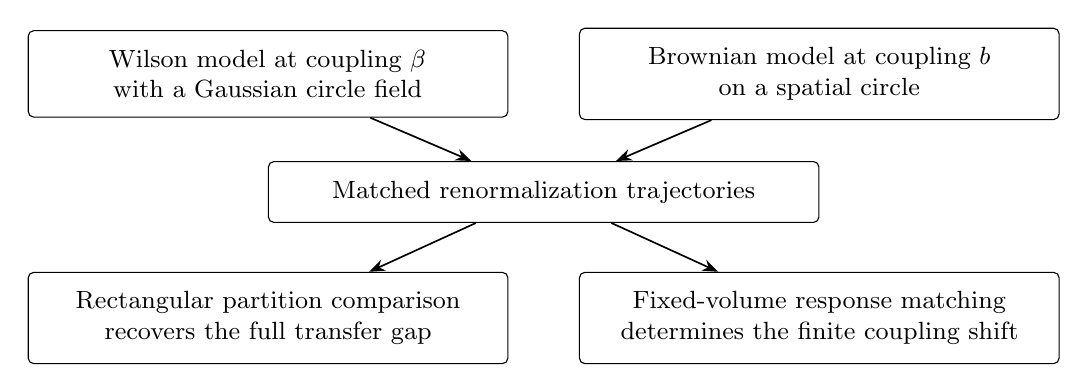
\begin{tikzpicture}[
  box/.style={draw,rounded corners=2pt,align=center,inner sep=7pt,
              font=\small,text width=5.6cm},
  arrow/.style={-{Stealth[length=2mm]},semithick}]
  \node[box] (wilson) at (-3.5,0)
    {Wilson model at coupling \(\beta\)\\with a Gaussian circle field};
  \node[box] (brownian) at (3.5,0)
    {Brownian model at coupling \(b\)\\on a spatial circle};
  \node[box,text width=6.5cm] (matching) at (0,-1.5)
    {Matched renormalization trajectories};
  \node[box] (partition) at (-3.5,-3.1)
    {Rectangular partition comparison\\
     recovers the full transfer gap};
  \node[box] (response) at (3.5,-3.1)
    {Fixed-volume response matching\\
     determines the finite coupling shift};
  \draw[arrow] (wilson) -- (matching);
  \draw[arrow] (brownian) -- (matching);
  \draw[arrow] (matching) -- (partition);
  \draw[arrow] (matching) -- (response);
\end{tikzpicture}

 \caption{The two outputs of regulator matching. The partition estimate
 is used on growing rectangles, while the response comparison is obtained
 from a fixed-volume expansion before the volume is increased. Both follow
 from the matched trajectories; the response comparison is not obtained by
 differentiating the partition error bound.}
 \label{fig:comparison}
\end{figure}
Figure~\ref{fig:comparison} separates these two uses of the matching
construction and their different orders of limits.

\subsection{Organization and conventions}

Sections~\ref{sec:sector} and~\ref{sec:cylinders} establish the full-gap
comparison and its finite-volume form. Sections~\ref{sec:brownian}
and~\ref{sec:integral} construct the auxiliary regulator and solve the
integral equations governing its mass scale. Section~\ref{sec:bethe}
proves the finite-circle spectral formula. Section~\ref{sec:rg} develops
the exact renormalization comparison, and Sections~\ref{sec:initialization}
and~\ref{sec:comparison} initialize the Brownian density, match its
trajectory, and integrate the terminal comparison.
Section~\ref{sec:renormalization} computes the finite coupling shift.
Section~\ref{sec:assembly} completes the proof, including the required
particle-number and error estimates.

Throughout, \(c,C>0\) may change from line to line. Dependence on a fixed
parameter is indicated when it matters. We use \(f\asymp g\) for two-sided
bounds by positive constants independent of the parameter tending to its
limit, and \(f\sim g\) when \(f/g\to1\). The letter \(L\) below denotes
the fixed dyadic blocking factor, rather than the torus side \(L_0\) used
in \eqref{eq:gibbs}. Particle number is written \(n_p\); \(N\) denotes
renormalization depth. The two lattice coordinates are denoted by \(t,x\)
once rectangular volumes are introduced.

\section{Spin correlations and the full transfer spectrum}
\label{sec:sector}

A partition function counts every transfer eigenvalue, whereas a spin
two-point function sees only states created by a spin component.
We first relate these two measurements. The key estimate is
finite-dimensional: the covariance of two even spin monomials is
quadratic in the largest component two-point function between their
supports. The proof adapts the three-component argument of
\cite[Section~4]{O3Pole}, replacing its conditional Ising--rotator
decomposition by two conditional rotators. We include the proof because
its treatment of several spin components is essential for the full gap.

Here a monomial is a product of individual spin components with
coefficient one. Its site list has one entry for each factor,
including repetitions.

\subsection{Conditional rotators and correlation signs}

Let $\mathcal G=(V,E)$ be a finite graph and give $q_x\in S^3$, $x\in V$,
the probability law
\begin{equation}
 d\nu_J(q)=Z_J^{-1}
 \exp\left(\sum_{xy\in E}J_{xy}q_x\cdot q_y\right)
 \prod_{x\in V}d\omega_3(q_x),
 \qquad J_{xy}\ge0.
 \label{eq:wilson-graph-law}
\end{equation}
There is no external field and no pinned boundary. We write
$\mathbb E_J$ for this expectation.

We recall the finite-system inequalities used below. For a zero-field
ferromagnetic plane rotator with angles $\theta_x$, every two integer
vectors $k,l$ indexed by $V$ satisfy
\begin{equation}
 \mathbb E\cos(k\cdot\theta)\ge0,\qquad
 \operatorname{Cov}\bigl(\cos(k\cdot\theta),
                         \cos(l\cdot\theta)\bigr)\ge0.
 \label{eq:wilson-xy-ginibre}
\end{equation}
These are the plane-rotator inequalities of Ginibre
\cite{Ginibre1970}. For clarity, the needed version has a short
replica proof. Fourier expansion with nonnegative coefficients gives
the first assertion. For the second, take independent copies
$\theta,\theta'$ and substitute
$\theta=\varphi+\psi$, $\theta'=\varphi-\psi$. This surjective
homomorphism of product tori preserves Haar integration. Each
observable difference becomes
$-2\sin(k\cdot\varphi)\sin(k\cdot\psi)$, and the replicated weight is
\[
 \exp\left(2\sum_{xy\in E}J_{xy}
       \cos(\varphi_x-\varphi_y)\cos(\psi_x-\psi_y)\right).
\]
Expanding it expresses twice the covariance as a sum of squares of
real integrals with nonnegative coefficients. Absolute convergence
holds on the finite graph. Differentiating a cosine mean in a bond
coupling consequently shows that the mean is nondecreasing in that
coupling. We also use the zero-field Ising GKS inequalities
\cite{KellySherman1968}:
sign-monomial means and their covariances are nonnegative.
These are precisely the finite-system ingredients of the conditional
argument in \cite[Section~3.11]{SharpO4}.

A law of real variables is \emph{associated} if any two bounded
coordinatewise increasing functions have nonnegative covariance.
At every vertex write
\begin{equation}
 q_x=\bigl(\cos\alpha_x\cos\theta_x,\,
           \cos\alpha_x\sin\theta_x,\,
           \sin\alpha_x\cos\phi_x,\,
           \sin\alpha_x\sin\phi_x\bigr),
 \qquad 0\le\alpha_x\le\frac{\pi}{2}.
 \label{eq:wilson-two-planes}
\end{equation}
The sphere prior is the product of the two uniform circle laws and
$\sin(2\alpha_x)\,d\alpha_x$. Given $\alpha$, the two circle systems
are independent and have couplings
\[
 J^L_{xy}=J_{xy}\cos\alpha_x\cos\alpha_y,\qquad
 J^R_{xy}=J_{xy}\sin\alpha_x\sin\alpha_y.
\]

\begin{lemma}[Association and single-component signs]
\label{lem:wilson-signs}
The $\alpha$ marginal in \eqref{eq:wilson-two-planes} is associated.
For two even-degree monomials each using a single spin component,
the covariance is nonnegative when their components agree and
nonpositive when they differ. The same signs hold for the two
components of a zero-field ferromagnetic plane rotator.
\end{lemma}

\begin{proof}
The density of $\alpha$ relative to its product one-site prior is
proportional to $Z_L(\alpha)Z_R(\alpha)$. For either factor, denote
its bond observables by $O_e$ and its couplings by $J_e(\alpha)$.
At two distinct vertices,
\[
 \partial_x\partial_y\log Z
 =\sum_e\mathbb E(O_e)\,\partial_x\partial_yJ_e
 +\sum_{e,f}\operatorname{Cov}(O_e,O_f)
                  \partial_xJ_e\,\partial_yJ_f.
\]
All first coupling derivatives in the left plane are nonpositive;
all those in the right plane are nonnegative. A nonzero mixed
derivative at distinct vertices occurs only at a bond's endpoints
and is nonnegative. The bond means and covariances are nonnegative
by \eqref{eq:wilson-xy-ginibre}. Thus the logarithmic density has
nonnegative mixed derivatives. It satisfies the FKG lattice
condition and hence is associated \cite{FortuinKasteleynGinibre1971}.
For this continuous array, restrict to compact subintervals of
$(0,\pi/2)$, apply the finite-grid FKG inequality to approximating
densities, and pass to the limit. Bounded increasing functions follow
by approximation and the usual monotone-class extension. The endpoint
restrictions can then be removed.

For the plane-rotator assertion, write its components as
$(\varepsilon\cos\gamma,\varepsilon'\sin\gamma)$,
$0\le\gamma\le\pi/2$. Given $\gamma$, the signs are independent
ferromagnetic Ising systems. The same mixed-derivative calculation
with GKS proves association of $\gamma$. Including amplitude factors,
the first-component monomial mean is nonnegative and decreasing in
$\gamma$, while the second-component mean is nonnegative and
increasing. Conditional independence gives the nonpositive covariance
for unlike components. For like components, the conditional covariance
is nonnegative by GKS and the covariance of conditional means is
nonnegative by association.

In \eqref{eq:wilson-two-planes}, a component-one monomial has
conditional mean equal to its cosine amplitudes times a nonnegative
linear combination of cosine-character means. It is nonnegative and
decreasing in $\alpha$. A component-four monomial has a nonnegative
increasing conditional mean, by a fixed rotation of the right circle.
Conditional independence gives the nonpositive covariance between
these components. For like components, the conditional covariance
is nonnegative by \eqref{eq:wilson-xy-ginibre}; the conditional means
have the same monotonicity. Component symmetry supplies the remaining
choices of components.
\end{proof}

\subsection{The covariance comparison}

\begin{proposition}[Finite-graph sector comparison]
\label{prop:wilson-covariance}
For the law \eqref{eq:wilson-graph-law}, let $P,Q$ be spin monomials
of positive degrees $r,s$ with site lists $\mathcal X,\mathcal Y$,
and put
\[
 G=\max_{x\in\mathcal X,\ y\in\mathcal Y}\mathbb E_J(q_x^1q_y^1).
\]
Then $G\ge0$, and a constant $C_{r,s}$ depending only on the degrees
satisfies
\begin{equation}
 |\operatorname{Cov}_J(P,Q)|\le C_{r,s}
 \begin{cases}
  G^2,&r,s\ \text{even},\\
  G,&r,s\ \text{odd},\\
  0,&r+s\ \text{odd}.
 \end{cases}
 \label{eq:sector-cov}
\end{equation}
If either monomial is constant, its covariance is zero. The estimate
is independent of the finite graph and its nonnegative couplings.
\end{proposition}

\begin{proof}
We first control coefficients in the positive pairing expansion.
This treats the odd case and several even cases. For the remaining
case we must also control the covariance of conditional means.

The uniform sphere moment tensor vanishes in odd degree, and
in degree $2h$ it is
\[
 \int_{S^3}q^{i_1}\cdots q^{i_{2h}}\,d\omega_3(q)
 =\frac{1}{4\cdot6\cdots(4+2h-2)}
   \sum_{\pi}\prod_{\{b,c\}\in\pi}\mathbf1_{\{i_b=i_c\}},
\]
where the sum runs over pairings of labeled factors. Expand each
bond exponential in powers of the dot product and apply the tensor
identity at each site. Following the contracted bond lines pairs
the external factors, and every closed line contributes four.
Thus, for arbitrary assigned external components,
\begin{equation}
 \mathbb E_J\prod_{b=1}^{r+s}q_{x_b}^{i_b}
 =\sum_\pi d_\pi
       \prod_{\{b,c\}\in\pi}\mathbf1_{\{i_b=i_c\}},
 \qquad d_\pi\ge0.
 \label{eq:wilson-pairings}
\end{equation}
The $d_\pi$ do not depend on the component assignment.
Repeated sites cause no difficulty because the factors remain
labeled. Absolute convergence justifies regrouping the expansion.
In particular the component two-point functions are nonnegative.

A pair is \emph{crossing} if it joins $\mathcal X$ to $\mathcal Y$.
When $r,s$ are odd, every pairing crosses. Fix one crossing pair
and assign component four to its endpoints and component one to
all remaining endpoints. The resulting moment contains $d_\pi$
as a nonnegative summand. Conditional on $\alpha$, the remaining
left-plane monomial has mean in $[0,1]$, including all amplitudes.
Its removal bounds the moment by the chosen component-four pair
mean. Hence $d_\pi\le G$. Both separate monomial means vanish
in odd total degree, so summing the pairing coefficients proves
the odd case.

When $r,s$ are even, every crossing pairing has at least two
crossing pairs. Assign component four to one, component two to
another, and component one to the remaining endpoints.
In the left plane, Lemma~\ref{lem:wilson-signs} bounds the joint
mean of the component-two pair and the component-one monomial
by the product of their nonnegative means. The latter monomial
mean and its amplitudes are at most one. The surviving
component-two pair mean, including its amplitudes, is decreasing
in $\alpha$, because
\[
 \mathbb E(\sin\theta_x\sin\theta_y\mid\alpha)
 =\tfrac12\mathbb E(\cos(\theta_x-\theta_y)\mid\alpha).
\]
This also holds when $x=y$. The component-four pair mean is
increasing in $\alpha$. Association bounds their product
expectation by the product of the full pair means, each at most $G$.
Therefore
\begin{equation}
 d_\pi\le G^2
 \quad\text{for every crossing pairing of two even lists}.
 \label{eq:wilson-crossing}
\end{equation}

For two single-component even monomials, compare equal and
different choices of their components. The products of their
means agree by symmetry. Their joint moments differ by exactly
the crossing contributions in \eqref{eq:wilson-pairings}.
By Lemma~\ref{lem:wilson-signs}, the two covariances have opposite
weak signs, so each absolute covariance is at most this difference.
Equation~\eqref{eq:wilson-crossing} proves the bound. The same
reasoning applies to every pair of even sublists with the
original value of $G$. If $P$ or $Q$ has odd degree in some
component, its separate mean is zero and every compatible
joint pairing crosses. This also follows from
\eqref{eq:wilson-crossing}.

It remains to consider monomials even in every component.
We use single-component replacements, whose full covariances are already
controlled, to bound both terms in the conditional covariance decomposition.
Write $P=P_LP_R$ by its two planes and put
\[
 b_{P,L}=\mathbb E(P_L\mid\alpha),\qquad
 b_{P,R}=\mathbb E(P_R\mid\alpha).
\]
Let $P_L^*$ replace all its components by component one and
$P_R^*$ replace all its components by component three. Denote
their conditional means by $B_{P,L},B_{P,R}$ and use the
corresponding notation for $Q$. Then
\[
 |b_{P,L}|,|b_{P,R}|\le1,\qquad
 0\le B_{P,L},B_{P,R}\le1,
\]
with $B_{P,L}$ decreasing and $B_{P,R}$ increasing in $\alpha$.

Factor the common amplitude $A_P(\alpha)$ from the left plane.
Its Fourier expansion and the expansion after replacement are
\[
 P_L=A_P(\alpha)\sum_k c_k\cos(k\cdot\theta),\qquad
 P_L^*=A_P(\alpha)\sum_k d_k\cos(k\cdot\theta),\qquad
 |c_k|\le d_k.
\]
Each sine or cosine supplies two exponential terms of modulus
$1/2$. Since the total number of sine factors is even, the
original coefficients are real and invariant under $k\mapsto-k$.
Replacement changes their phases to positive coefficients.
Collecting equal frequencies preserves their domination,
including for repeated sites. The same argument applies in
the right plane. By \eqref{eq:wilson-xy-ginibre},
\begin{equation}
 |\operatorname{Cov}(P_L,Q_L\mid\alpha)|
 \le\operatorname{Cov}(P_L^*,Q_L^*\mid\alpha),
 \label{eq:wilson-fourier-covariance}
\end{equation}
and likewise for $R$.

Conditional independence gives
\begin{align*}
 \operatorname{Cov}(P,Q\mid\alpha)
 ={}&\operatorname{Cov}(P_L,Q_L\mid\alpha)
                    \mathbb E(P_RQ_R\mid\alpha)\\
 &+b_{P,L}b_{Q,L}\operatorname{Cov}(P_R,Q_R\mid\alpha).
\end{align*}
The other factors have modulus at most one, so its averaged
absolute value is at most
\[
 \mathbb E\operatorname{Cov}(P_L^*,Q_L^*\mid\alpha)
 +\mathbb E\operatorname{Cov}(P_R^*,Q_R^*\mid\alpha).
\]
Each term is at most its full single-component covariance:
the omitted covariance of conditional means is nonnegative
by association. Both terms have already been bounded by
$C_{r,s}G^2$.

We still need the covariance of the conditional means.
The Fourier comparison shows that $B_{P,L}\pm b_{P,L}$ are
nonnegative combinations of cosine-character means multiplied
by their common amplitude. Both are decreasing; likewise
$B_{P,R}\pm b_{P,R}$ are increasing. For
$\alpha\le\widetilde\alpha$ this gives
\[
 |b_{P,L}(\widetilde\alpha)-b_{P,L}(\alpha)|
 \le B_{P,L}(\alpha)-B_{P,L}(\widetilde\alpha),
\]
and the corresponding increasing bound for the right plane.
The factors $b_{P,R},b_{P,L}$ in the conditional mean need not be monotone.
Their changes are nevertheless
bounded by those of the increasing $B_{P,R}$ and decreasing $B_{P,L}$.
To combine these two controls, put
\[
 Y_P=b_{P,R}b_{P,L},\qquad D_P=B_{P,R}-B_{P,L}.
\]
Using the modulus bounds on the $b$ functions yields
\[
 |Y_P(\widetilde\alpha)-Y_P(\alpha)|
 \le D_P(\widetilde\alpha)-D_P(\alpha).
\]
Consequently $D_P+Y_P$ and $D_P-Y_P$ are increasing.
Apply association to these functions and to $D_Q\pm Y_Q$.
Adding the two matching-sign inequalities and the two
opposite-sign inequalities proves
\begin{equation}
 |\operatorname{Cov}(Y_P,Y_Q)|
 \le\operatorname{Cov}(D_P,D_Q).
 \label{eq:wilson-conditional-means}
\end{equation}
On expanding the right side, the two same-plane terms are
bounded by their full single-component covariances, as above.
The two opposite-plane terms are exactly full single-component
covariances by conditional independence; they enter with minus
signs. Each is bounded in absolute value by the estimate already
proved on even sublists. Empty sublists give constants and zero
covariances. The total-covariance identity now proves the even case.

Finally, global spin inversion makes the joint moment zero
when $r+s$ is odd, and at least one separate mean is zero.
This proves all cases of \eqref{eq:sector-cov}.
\end{proof}

\subsection{Consequences for the plane and finite cylinders}

An observable is \emph{even} or \emph{odd} according to its parity
under simultaneous inversion $q_x\mapsto-q_x$ at every site.
A \emph{component reflection} reverses one fixed component at
every site and leaves the others unchanged. The same definitions
apply on a row. Thus total inversion is the product of the four
commuting component reflections; being even under total inversion
does not require being even under each of them.

For the original Wilson law, we write $q=\sigma$ and
$m(\beta)=m_{\mathrm{lat}}(\beta)$. Let $r_*(\beta)$ be the
supremum of the support of the $T_\beta$-spectral measure of
$[q_0^1]$ in the OS Hilbert space of Section~\ref{sec:introduction}.

\begin{proposition}[The spin field sees the full gap]
\label{prop:wilson-full-gap}
For every $\beta>0$, in the periodic plane state,
\begin{equation}
 m(\beta)=-\log r_*(\beta)
 =-\log\lim_{n\to\infty}
       \bigl(\mathbb E_{\mu_\beta}q_0^1q_{(n,0)}^1\bigr)^{1/n}.
 \label{eq:full-gap}
\end{equation}
The transfer norm on the even subspace orthogonal to the vacuum
is at most $r_*(\beta)^2$. Its gap is therefore at least
$2m(\beta)$. The logarithms can be read in the extended sense;
the imported upper bound below makes them finite throughout
the large-$\beta$ regime.
\end{proposition}

\begin{proof}
The finite-graph estimate passes to the periodic plane limit
for fixed monomials. Spatial translations are unitary in the
OS form and commute with $T_\beta$. Translated one-spin vectors
have the same spectral support. Thus OS Cauchy--Schwarz gives
\[
 0\le\mathbb E_{\mu_\beta}
       (q_{(0,x)}^1q_{(n,y)}^1)\le\tfrac14r_*^n
\]
for arbitrary spatial sites $x,y$. The factor $1/4$ is their
one-site reflection norm squared.

A reflected polynomial transfer autocorrelation is a finite
sum of monomial covariances at temporal separation at least
$n$. For an odd polynomial, \eqref{eq:sector-cov} bounds it by
$C_P r_*^n$; for a centered even polynomial it bounds it by
$C_P r_*^{2n}$. The spectral measures are positive, so their
supports lie in $[0,r_*]$ and $[0,r_*^2]$, respectively.
Polynomials on a fixed finite spin product are dense in the
$L^2$ space of its marginal law. Reflection invariance gives
$\|[F]\|_{\mathrm{OS}}^2\le\mathbb E|F|^2$, so this approximation
also holds in the OS seminorm. Centering and parity
symmetrization preserve density. Bounded spectral projections
extend the spectral bounds to the full subspaces.
Since $[q_0^1]$ is centered, the full nonvacuum norm is exactly
$r_*$. Finally, the $n$th root of a moment of a positive
spectral measure tends to the supremum of its support.
This proves \eqref{eq:full-gap}.
\end{proof}

For even integers $n,\ell\ge4$, let $Z_\beta(n,\ell)$ denote the Wilson partition function on
the rectangular torus with $n$ time sites and $\ell$ spatial
sites, with the same single-counted bonds and probability spin
measure as in Section~\ref{sec:introduction}.
For an even spatial circumference $\ell\ge4$, let
$\mathscr X_\ell=(S^3)^\ell$ with product probability measure.
Put $V_\ell(s)=\sum_{i=1}^{\ell}s_i\cdot s_{i+1}$, periodically,
and define the row transfer kernel
\begin{equation}
 K_{\beta,\ell}(s,s')
 =\exp\left[\frac{\beta}{2}V_\ell(s)
       +\beta\sum_{i=1}^{\ell}s_i\cdot s'_i
       +\frac{\beta}{2}V_\ell(s')\right].
 \label{eq:wilson-row-kernel}
\end{equation}
It is compact, with a continuous strictly positive kernel
and a simple top eigenvalue $\lambda_1$.
The tensor-power expansion of $e^{\beta s\cdot s'}$
makes it positive semidefinite and trace class. Write
\[
 U_{\beta,\ell}=K_{\beta,\ell}/\lambda_1,\qquad
 \Omega_{\beta,\ell}>0,\quad\|\Omega_{\beta,\ell}\|_2=1,\qquad
 \tau_{\beta,\ell}=\lambda_2/\lambda_1.
\]
For $\beta>0$ the kernel is not rank one, as its cross ratios
vary with the row configurations. Hence $0<\tau_{\beta,\ell}<1$.
Closing time gives
$Z_\beta(n,\ell)=\operatorname{Tr}K_{\beta,\ell}^{\,n}$.
These are the conventions of \cite[Section~2.1]{SharpO4}.
Denote the infinite-time cylinder expectation by
$\omega_{\beta,\ell}$.

\begin{lemma}[An odd detector for the first cylinder excitation]
\label{lem:wilson-detector}
The restriction of $U_{\beta,\ell}$ to the centered even row
subspace has norm at most $\tau_{\beta,\ell}^2$. There is a real
row function $F$, with $|F|\le1$, odd under reflection of one
spin component, such that
\begin{equation}
 \omega_{\beta,\ell}(F\,F\circ\vartheta_n)
 \ge\frac{\tau_{\beta,\ell}}{1+\tau_{\beta,\ell}}\,
                    \tau_{\beta,\ell}^{\,n},\qquad n\ge0,
 \label{eq:wilson-detector-overlap}
\end{equation}
where $\vartheta_n$ translates by $n$ rows.
\end{lemma}

\begin{proof}
The finite-graph estimate passes to the infinite-time cylinder
by the row transfer representation. Component vectors
$q_x^i\Omega$ are centered, so their correlations across $n$
rows are at most $\tau^n$, suppressing $\beta,\ell$.
The even polynomial estimate therefore places the spectral
support of every centered even polynomial vector in $[0,\tau^2]$.
Polynomials are uniformly
dense in continuous row functions, and the continuous positive
$\Omega$ has a positive minimum. Thus polynomials times $\Omega$
are dense in row space, proving the even-sector norm bound.

Choose a real unit $\tau$-eigenfunction $v$. Since
$\tau>\tau^2$, its eigenspace is odd under simultaneous inversion.
The four component reflections commute with one another and
with $U$, so $v$ can have definite parity under each; at least
one is odd. Relabel it as component one. The modulus $|v|$
is even. With $b_0=\langle\Omega,|v|\rangle^2$, positivity of
the kernel and the even-sector bound give
\[
 \tau\le\langle|v|,U|v|\rangle
       \le b_0+(1-b_0)\tau^2,
 \qquad b_0\ge\frac{\tau}{1+\tau}.
\]
Take $F=\operatorname{sgn}v$, equal to zero on its zero set.
Its overlap with $v$ is
$\langle v,F\Omega\rangle=\langle|v|,\Omega\rangle$.
Keeping this contribution in the positive spectral expansion
of its correlation proves \eqref{eq:wilson-detector-overlap}.
\end{proof}

The detector can involve the entire row. We next recover a
component correlation with a cost polynomial in the circumference.

\begin{lemma}[Visibility through component correlations]
\label{lem:wilson-visibility}
For fixed $\beta>0$ there is a finite constant $C_\beta$,
independent of even $\ell\ge4$, such that bounded row functions
$F,G$ of modulus at most one, both odd under reflection of
component one, satisfy
\begin{equation}
 |\omega_{\beta,\ell}(F\,G\circ\vartheta_n)|
 \le C_\beta\sum_{x\in R_0,\ y\in R_n}
                      \omega_{\beta,\ell}(q_x^1q_y^1),
 \qquad n\ge1.
 \label{eq:wilson-visibility}
\end{equation}
Here $R_0,R_n$ are the two rows of $\ell$ sites.
\end{lemma}

\begin{proof}
On a finite torus, write
\[
 q_i=(\varepsilon_i u_i,\sqrt{1-u_i^2}\,l_i),\qquad
 \varepsilon_i\in\{-1,1\},\quad u_i\in[0,1],\quad l_i\in S^2.
\]
The prior is a product: $\varepsilon_i$ is fair, $l_i$ is
uniform, and $u_i$ has density proportional to $\sqrt{1-u_i^2}$.
Given $u,l$, the signs are a ferromagnetic Ising model with
coupling $\beta u_i u_j$. In its Edwards--Sokal representation
\cite{EdwardsSokal1988}, an edge between equal signs is open
with probability $1-e^{-2\beta u_i u_j}$, and an edge between
different signs is closed. Given the edges, cluster signs
are independent and fair. If no cluster
joins the detector rows, flip all clusters touching the first
row. This reverses $F$ and leaves $G$ unchanged. Its conditional
product mean is therefore zero. The absolute detector
correlation is bounded by the row-connection probability,
and then by the sum of pair-connection probabilities.

For a pair $x,y$ the joint spin--edge representation gives
\begin{equation}
 \mathbb E(q_x^1q_y^1)
 =\mathbb E[u_xu_y\mathbf1_{\{x\leftrightarrow y\}}].
 \label{eq:wilson-fk-pair}
\end{equation}
Condition on all edges, directions $l$, and amplitudes other
than $u_i$. After summing the signs, each closed incident edge
has factor $e^{-J}$ and each open edge has factor $e^J-e^{-J}$,
where $J=\beta u_i u_j$. The cluster multiplicity depends only
on the fixed edges. Raising $u_i\in[0,1/4]$ to
$u_i+1/4\in[1/4,1/2]$ increases every open factor. Closed-edge
factors and perpendicular factors
\[
 \exp\bigl(\beta\sqrt{1-u_i^2}\sqrt{1-u_j^2}\,l_i\cdot l_j\bigr)
\]
change by bounded ratios depending only on $\beta$ and degree
four. The amplitude prior is bounded above and below on these
intervals. Comparing their integrals proves
\[
 \mathbb P(u_i\ge1/4\mid\text{all other data})\ge c_\beta>0
\]
uniformly in the volume. Applying this twice by the tower
property gives
$\mathbb E[u_xu_y\mid\text{edges},l]\ge c_\beta^2/16$.
The connection event is edge-measurable, so
\eqref{eq:wilson-fk-pair} bounds its probability by
$16c_\beta^{-2}\mathbb E(q_x^1q_y^1)$. Summing proves the
finite-torus estimate.

At fixed circumference the transfer representation converges
to the cylinder for all bounded Borel row insertions: separate
the ground projection, use their bounded multiplication norms,
and let the excited trace tail tend to zero. The estimate
therefore passes to the cylinder, including the sign detector.
\end{proof}

\section{Cylinder masses and a partition-function rate}
\label{sec:cylinders}

We now express the plane mass as the decay rate of a
volume-canceling combination of square partition functions.
Trace estimates will be uniform over the admitted cutoff
trajectories. In contrast, the visibility argument will be
applied only after fixing one trajectory and sending the
circumference to infinity.

\subsection{The imported Wilson trajectory bounds}

Here is the precise input from \cite{SharpO4}. Fix its
sufficiently large dyadic blocking factor $L$ and auxiliary
parameters, and then choose the terminal reference coupling
$H$ sufficiently large for its construction and mass bounds. Put
\[
 H_j=H+\frac{\log L}{\pi}j,\qquad I_H=[0.9H,1.1H].
\]
An \emph{admitted nearest-neighbor trajectory of depth $N$}
is the exact $N$-step block integration of the nearest-neighbor
Wilson law constructed in \cite[Sections~5.1 and~7.1]{SharpO4}.
At every remaining depth $j=N,\ldots,0$, its retained density
satisfies the controlled-class bounds in that source and its
kinetic coupling lies in $[H_j/2,2H_j]$. The kinetic coupling
is the coefficient extracted from the quadratic energy of a
slowly varying retained spin field. Its initial value is the
bare coupling $\beta$ and its final value is denoted by $h$.
No uniqueness of an admitted bare coupling with given $N,h$
is assumed. The trace argument will use only the numerical
conclusions of the following imported proposition.

\begin{proposition}[Wilson trajectory input]
\label{prop:wilson-input}
For each $N\ge1$ and $h\in I_H$ there exists an admitted
nearest-neighbor trajectory of depth $N$ ending at $h$.
Every sufficiently large bare coupling occurs in at least
one such trajectory. There are fixed integers $N_0,M_0>0$,
with $M_0$ dyadic, such that every admitted trajectory with
$N\ge N_0$, terminal coupling $h\in I_H$, bare coupling
$\beta$, and spacing $a=L^{-N}$ obeys
\begin{align}
 4\log Z_\beta(M_0/a,M_0/a)
 -\log Z_\beta(2M_0/a,2M_0/a)&\le2^{-10},
 \label{eq:wilson-seed}\\
 m(\beta)/a&\le\log8,
 \label{eq:wilson-input-upper}\\
 N\log L&=\pi\beta-\tfrac12\log\beta+O_{L,H}(1).
 \label{eq:wilson-calibration}
\end{align}
In particular $a\asymp_{L,H}\sqrt\beta e^{-\pi\beta}$.
The error bound and the two preceding inequalities are uniform
over these trajectories. The periodic plane limit is unique
and has a positive full OS gap for every fixed $\beta>0$.
\end{proposition}

\begin{proof}[Source and applicability]
Admission and coverage are \cite[Proposition~7.1]{SharpO4};
calibration is its Proposition~6.2. The seed
\eqref{eq:wilson-seed} is the concluding estimate in the proof
of its Theorem~9.2: the reference depth and then the dyadic
$M_0$ are fixed before the final depth varies. The upper bound
is its Proposition~10.2. Periodic-limit uniqueness and the
all-temperature full gap are its Theorem~1.1 and Corollary~1.2.
The sphere probability convention, single counting of bonds,
even periods, and site-reflection one-step transfer coincide
with ours. In particular the cited gaps concern the full local
OS space, including rotation-invariant observables.
\end{proof}

Fix one admitted trajectory with $N\ge N_0$ and $h\in I_H$
for the following definitions and suppress its parameters.
Physical lengths $t,w$ always have $t/a,w/a$
even integers at least four. Write
\[
 \mathcal Z(t,w)=Z_\beta(t/a,w/a),\qquad
 U(w)=U_{\beta,w/a},\qquad E(w)=-a^{-1}\log\tau_{\beta,w/a}.
\]
Define
\begin{align*}
 p(t,w)&=2\log\mathcal Z(t,w)-\log\mathcal Z(2t,w),\\
 \Delta(w)&=4\log\mathcal Z(w,w)-\log\mathcal Z(2w,2w),\\
 s(t,w)&=\operatorname{Tr}U(w)^{t/a}-1.
\end{align*}
The top-eigenvalue scalar cancels in $p$, and every
area-proportional free-energy term cancels in $\Delta$.

\begin{proposition}[Uniform cylinder and partition rates]
\label{prop:cylinder-rate}
\label{prop:wilson-partition-rate}
For all admitted trajectories of Proposition~\ref{prop:wilson-input}
with $N\ge N_0$ and terminal coupling $h\in I_H$, there are
constants $C_H,w_H<\infty$, independent of the trajectory,
such that every dyadic $w\ge w_H$ satisfies
\begin{equation}
 \left|E(w)-\frac{m(\beta)}a\right|\le C_Hw^{-1/4}
 \label{eq:wilson-cylinder-rate}
\end{equation}
and
\begin{equation}
 \left|-\frac{\log\Delta(w)}w-\frac{m(\beta)}a\right|
       \le C_Hw^{-1/4}.
 \label{eq:partition-rate}
\end{equation}
\end{proposition}

We first obtain uniform convergence of a truncated cylinder
rate from exact rectangle identities. We then identify its
limit with the plane gap and remove the truncation.

\subsection{Trace tails and rectangle identities}

The transfer eigenvalues give
\[
 p(t,w)=2\log(1+s(t,w))-\log(1+s(2t,w)).
\]
If $1=u_1\ge u_2\ge\cdots\ge0$ are the eigenvalues of $U(w)$, the
normalized trace weights at time $t$ are
$\eta_i=u_i^{t/a}/(1+s(t,w))$. Thus
$e^{-p(t,w)}=\sum_i\eta_i^2\le\eta_1=(1+s(t,w))^{-1}$.
In particular $p\ge0$. Rotation interchanges the two periods; substitution
in the definitions proves
\begin{equation}
 \begin{aligned}
 \Delta(w)&=2p(w,w)+p(w,2w),\\
 p(t,2w)&=2p(t,w)-2p(w,t)+p(w,2t),\\
 0\le p(t,w)&\le2s(t,w),\\
 s(t,w)&\le e^{p(t,w)}-1.
 \end{aligned}
 \label{eq:rectangle-identities}
\end{equation}
Also,
\begin{equation}
 e^{-tE(w)}\le s(t,w)
 \le s(t_0,w)e^{-(t-t_0)E(w)}\quad(t\ge t_0).
 \label{eq:wilson-trace-advance}
\end{equation}
If $p(t,w)\le1/4$, then $s\le pe^p$ gives
\begin{equation}
 e^{-tE(w)}\le2p(t,w),\qquad
 p(2t,w)\le4p(t,w)^2.
 \label{eq:wilson-squaring}
\end{equation}
For the second inequality use
$p(2t,w)\le2s(2t,w)\le2s(t,w)^2\le2p^2e^{2p}$.

We include the dyadic argument from
\cite[Proposition~2.2]{SharpO4}. If $\Delta(r)\le2^{-10}$,
then $p(r,2r)\le\Delta(r)$ and
$p(2r,2r)\le4\Delta(r)^2$. The rectangle identity gives
\[
 p(r,4r)\le2p(r,2r)+p(2r,2r)\le3\Delta(r).
\]
Squaring yields $p(2r,4r)\le36\Delta(r)^2$, hence
\[
 \Delta(2r)\le44\Delta(r)^2\le64\Delta(r)^2.
\]
All squaring steps are justified by $3\cdot2^{-10}<1/4$.
Starting with \eqref{eq:wilson-seed}, this proves on dyadic
$w=2^kM_0$, with uniform $c,C>0$,
\begin{equation}
 \Delta(w)\le Ce^{-cw},\qquad E(w)\ge c,\qquad
 s(w/2,w)\le Ce^{-cw}\quad(w\ge2M_0).
 \label{eq:wilson-basic-tails}
\end{equation}
Indeed $e^{-wE(w)}\le2p(w,w)\le\Delta(w)$, and
$p(w/2,w)\le\Delta(w/2)$ controls the half-time trace.

\begin{lemma}[Long rectangles]
\label{lem:wilson-long-rectangles}
Uniformly over admitted trajectories with $N\ge N_0$ and
$h\in I_H$, for all sufficiently large dyadic $t$ and dyadic $w\ge2t$,
\begin{equation}
 p(t,w)\le C(w/t)e^{-ct}.
 \label{eq:wilson-long-rectangle}
\end{equation}
\end{lemma}

\begin{proof}
At $w=2t$, $p(t,2t)\le\Delta(t)$. For widths $z=t,2t$,
advance the half-circumference estimate
\eqref{eq:wilson-basic-tails} to time $w$ using
\eqref{eq:wilson-trace-advance} and $E(z)\ge c$.
This gives $p(w,t)+p(w,2t)\le Ce^{-cw}$, after decreasing $c$.
The rectangle identity therefore gives
$p(t,2w)\le2p(t,w)+Ce^{-cw}$.
Iteration over dyadic widths proves the result.
\end{proof}

\subsection{Convergence of a truncated cylinder rate}

Choose dyadic $t\asymp w^{1/2}$ and $t_0\asymp w^{1/4}$,
with fixed implicit constants. At widths $W=w,2w$,
Lemma~\ref{lem:wilson-long-rectangles} makes
$s(t_0,W)\le1$ uniformly for all large $w$. Hence
\begin{equation}
 e^{-tE(W)}\le s(t,W)\le e^{-(t-t_0)E(W)},\qquad
 \tfrac12s(t,W)\le p(t,W)\le2s(t,W).
 \label{eq:wilson-short-time-sandwich}
\end{equation}
The lower bound uses $p\ge\log(1+s)\ge s/2$ when $s\le1$.

We do not yet have a uniform upper bound for $E(W)$.
For fixed $B>0$, set
\[
 f_B(t,W)=-\frac1t\log\bigl(p(t,W)+e^{-Bt}\bigr).
\]
The preceding sandwich proves
\begin{equation}
 f_B(t,W)=\min\{E(W),B\}+O_B(w^{-1/4}).
 \label{eq:wilson-capped-rate}
\end{equation}
Its upper and lower exponential rates are
$\min\{E(W),B\}$ and
$\min\{(1-t_0/t)E(W),B\}$, up to $O(1/t)$.
Their difference is at most $Bt_0/t$, even if $E(W)>B$.

The swapped terms in the rectangle identity are $O(e^{-cw})$,
so $p(t,2w)=2p(t,w)+O(e^{-cw})$. The added $e^{-Bt}$ bounds
both logarithm arguments below, and $t\asymp\sqrt w$ makes
the additive error negligible. The factor two changes their
logarithms by at most a constant. Thus
$|f_B(t,2w)-f_B(t,w)|\le C_B/t$, and
\[
 |\min\{E(2w),B\}-\min\{E(w),B\}|\le C_Bw^{-1/4}.
\]
This is summable along dyadic doublings. The truncated rate
has a limit for each trajectory, with convergence error
$O_B(w^{-1/4})$ uniform over all trajectories.

\subsection{Identification with the plane gap}

For each fixed trajectory we first prove
\begin{equation}
 m(\beta)/a\ge\limsup_{w\to\infty}E(w),
 \label{eq:wilson-first-gap-direction}
\end{equation}
with dyadic widths. If $F$ is a bounded continuous observable
in a time slab of $r$ lattice steps, its normalized transfer
insertion $A_F$ has norm at most $\|F\|_\infty$. For $r=0$ it is
multiplication by $F$; for $r\ge1$ its kernel is pointwise dominated
in modulus by $\|F\|_\infty U(w)^r$.
For two such insertions, let $d$ be the number of lattice steps from
the last row of the first slab to the first row of the second. Then
\[
 |\operatorname{Cov}_{\omega_{\beta,w/a}}(F,G)|
 \le\|F\|_\infty\|G\|_\infty e^{-adE(w)}.
\]
The square-torus expectation of $F$ is
\[
 \frac{\operatorname{Tr}(A_F U(w)^{\,w/a-r})}
      {\operatorname{Tr}U(w)^{\,w/a}}.
\]
When $ar\le w/2$, separating the ground projection in
numerator and denominator bounds its difference from the
cylinder expectation by $2\|F\|_\infty s(w/2,w)$.
By \eqref{eq:wilson-basic-tails}, cylinders and square tori
therefore have the same local limits, namely the unique
periodic plane state.

Take a subsequence realizing the limsup of $E(w)$ and pass
the slab inequality to the plane. Applied to reflected local
autocorrelations, positivity of their spectral measures and
density in the OS space prove
\eqref{eq:wilson-first-gap-direction}. An infinite limsup would
give an infinite gap by the same argument, contradicting
\eqref{eq:wilson-input-upper}.

Take $B=10$ in the truncated-rate convergence. Its limit
is at most $\log8<10$, by
\eqref{eq:wilson-first-gap-direction} and
\eqref{eq:wilson-input-upper}. Uniform convergence makes the
truncation inactive for all sufficiently large widths,
uniformly over the trajectories. Thus
\begin{equation}
 E_\infty=\lim_{w\to\infty}E(w),\qquad
 |E(w)-E_\infty|\le C_Hw^{-1/4},\qquad
 E_\infty\le m(\beta)/a\le\log8.
 \label{eq:wilson-cylinder-limit}
\end{equation}

For the reverse inequality, fix $\beta,a$ and keep
$t\asymp\sqrt w$. Apply Lemmas~\ref{lem:wilson-detector}
and~\ref{lem:wilson-visibility} at $n=t/a$.
Since $E(w)$ is bounded, $\tau_{\beta,w/a}=e^{-aE(w)}$
and the detector overlap are bounded below by positive
constants for this fixed trajectory. Some pair on the two
rows therefore has correlation
\begin{equation}
 \omega_{\beta,w/a}(q_x^1q_y^1)
 \ge c_\beta'(w/a)^{-2}e^{-tE(w)}.
 \label{eq:wilson-visible-pair}
\end{equation}
The positive constant is independent of $w$.

Lift the spatial pair along a shortest circle arc. Its spatial
span is at most $w/2$, and its temporal span $t$ is also at most
$w/2$ for large $w$. The cylinder expectation and its plane
counterpart satisfy
\begin{equation}
 \left|\omega_{\beta,w/a}(q_x^1q_y^1)
       -\mathbb E_{\mu_\beta}(q_{\widetilde x}^1
                             q_{\widetilde y}^1)\right|
 \le Ce^{-cw},
 \label{eq:wilson-pair-to-plane}
\end{equation}
as follows. First compare the cylinder to the $w$ by $w$
torus by the slab estimate, with error at most $2s(w/2,w)$.
Compare the $w$ by $w$ and $2w$ by $w$ tori through their
common width-$w$ cylinder. Next rotate and compare the
$2w$ by $w$ and $2w$ by $2w$ tori through the width-$2w$
cylinder. The latter error is bounded by a constant times
$s(w/2,2w)=O(e^{-cw})$, using
Lemma~\ref{lem:wilson-long-rectangles}. Translations fit the
product into the required arcs at every comparison.
Repeat these two-direction doublings. Their errors sum to
$Ce^{-cw}$. For each initial $w$, the lifted observable is
fixed throughout the larger-torus limit, so periodic local
convergence proves \eqref{eq:wilson-pair-to-plane}.

Because $t\asymp\sqrt w$ and $E(w)$ is bounded, this error
is negligible relative to the right side of
\eqref{eq:wilson-visible-pair} as $w\to\infty$ at the fixed
trajectory. The plane component pair is at most
$e^{-m(\beta)t/a}$ by Proposition~\ref{prop:wilson-full-gap},
regardless of its spatial separation. Taking logarithms gives
\[
 m(\beta)/a
 \le E(w)+\frac{2\log(w/a)-\log(c_\beta'/2)}{t}.
\]
The extra term tends to zero, so $m(\beta)/a\le E_\infty$.
Together with \eqref{eq:wilson-cylinder-limit}, this proves
equality and \eqref{eq:wilson-cylinder-rate}. The fixed-trajectory
argument removed the nonuniform visibility constants; the
convergence rate was already uniform.

\begin{proof}[Completion of Proposition~\ref{prop:cylinder-rate}]
Apply \eqref{eq:wilson-trace-advance} at time $w$, with
$t_0\asymp w^{1/4}$ and widths $W=w,2w$.
The long-rectangle bound gives $s(t_0,W)\le1$, and hence
\[
 e^{-wE(W)}\le s(w,W)\le e^{-(w-t_0)E(W)}.
\]
Now $E(W)$ is uniformly bounded and $p(w,W)$ lies between
$s(w,W)/2$ and $2s(w,W)$. Therefore
\[
 -w^{-1}\log p(w,W)
 =E(W)+O_H(w^{-3/4})
 =m(\beta)/a+O_H(w^{-1/4}).
\]
The positive sum $\Delta(w)=2p(w,w)+p(w,2w)$ has the same
logarithmic rate within this error. This proves
\eqref{eq:partition-rate}.
\end{proof}

\section{The Brownian regulator and its transfer operators}
\label{sec:brownian}

The partition comparison used later introduces a model with continuous space
and discrete time.  We first construct its transfer operators and identify the
state on which their norms can be calculated.  The circumference remains
finite throughout.  This point is essential: the comparison with the lattice
model will require a quantitative statement on a specified, growing family
of circles.

\subsection{The row measure and particle expansion}

Let space be the circle $\mathbb R/W\mathbb Z$, where $W>0$, and let one unit
of discrete time be a vertical lattice step.  The spin manifold is
\[
 \mathcal G=(\mathbb R/2\pi\mathbb Z\times SU(2))/
       \bigl((v,Q)\sim(v+\pi,-Q)\bigr),
 \qquad G=e^{iv}Q.
\]
We identify $SU(2)$ with the unit sphere $S^3$.  On a row, use the
unnormalized Brownian loop measure with Hamiltonian
\[
 E=\frac12\bigl(-\partial_v^2-\Delta_{S^3}\bigr),
\]
with Haar probability as reference measure.  Thus the mass of the row
measure is $\operatorname{Tr}e^{-WE}$.  We denote integration with respect to
this measure by $\mathcal E_W$.  For $b>0$, set $\lambda=b^2/2$ and assign
successive rows the oriented interaction
\[
 \exp\left\{\lambda\int_0^W
                \operatorname{Tr}\bigl(G_t(x)G_{t+1}(x)^*\bigr)\,dx\right\}.
\]
Reversing the orientation complex-conjugates the interaction and gives the
same construction after reversing the notation for successive rows.

We use $n_{\mathrm p}$ exclusively for particle number, reserving $N$ for the
renormalization depth later in the paper.  Expand each vertical exponential.
A constant circle rotation on one row multiplies its incoming and outgoing
terms by opposite circle characters.  Integration over that rotation
therefore forces the same particle number on every time-link.  A color
$A_i=(a_i^L,a_i^R)\in\{1,2\}^2$ records the two matrix indices of the $i$th
insertion.  The particle Hilbert space is the bosonic subspace of
\[
 L^2\bigl((\mathbb R/W\mathbb Z)^{n_{\mathrm p}};
                     (\mathbb C^2\otimes\mathbb C^2)^{\otimes n_{\mathrm p}}\bigr).
\]
Equivalently, we integrate positions over the ordered chamber
$0<X_1<\cdots<X_{n_{\mathrm p}}<W$, with the color identifications induced
by simultaneous permutation of particles.  All kernels below act by
integration over this chamber and summation over colors.  The chamber
integral therefore absorbs the factorial in the exponential series.

For position and color lists $(X,A)$ and $(Y,B)$, define
\begin{equation}
 T_{n_{\mathrm p}}(Y,B;X,A)
 =\lambda^{n_{\mathrm p}}\mathcal E_W\left[
       \prod_{i=1}^{n_{\mathrm p}}G_{B_i}(Y_i)
                        \overline{G_{A_i}(X_i)}\right].
 \label{eq:brownian-transfer}
\end{equation}
For time period $n$, the periodic partition function is
\[
 Z^B_+(n,W)=\sum_{n_{\mathrm p}\ge0}
                   \operatorname{Tr}T_{n_{\mathrm p}}^{\,n}.
\]
A minus-center seam in time multiplies each term by $(-1)^{n_{\mathrm p}}$.
The expansion is absolutely convergent at every finite period.  Each
$T_{n_{\mathrm p}}$ is a positive operator: its kernel is the Gram kernel of
the insertion functions in the row loop measure.  Moreover,
\[
 \sum_{n_{\mathrm p}\ge0}\operatorname{Tr}T_{n_{\mathrm p}}
 =e^{2\lambda W}\operatorname{Tr}e^{-WE}<\infty,
\]
because $\sum_{a,b}|G_{ab}|^2=2$.  In particular, for each parity
$\ell\in\{0,1\}$ the maximum
\[
 \tau_\ell=\max_{n_{\mathrm p}\equiv\ell\ ({\rm mod}\ 2)}
                              \|T_{n_{\mathrm p}}\|
\]
is attained.

\begin{proposition}[The parity norm difference]
\label{prop:brownian-parity}
Let $b\to\infty$, and suppose that for a fixed $D>0$
\[
 W\asymp e^{\pi b}b^{-1/2}(\log b)^D.
\]
Suppose also that there is a fixed $C_*>0$ such that every particle number
attaining either parity maximum satisfies
$|n_{\mathrm p}/W-b^2|\le C_*b$.  Then
\begin{equation}
 \log\tau_0-\log\tau_1
       \sim32\sqrt2\,b^{1/2}e^{-\pi b}.
 \label{eq:B1}
\end{equation}
\end{proposition}

The remainder of this section identifies the relevant eigenstate.
Section~\ref{sec:integral} determines the scalar quantity that will give
\eqref{eq:B1}, and Section~\ref{sec:bethe} completes the finite-circle
spectral calculation.  The particle-number hypothesis will be verified
when the Brownian and Wilson partition functions are compared.

\subsection{Positivity and a commuting contact Hamiltonian}

The two copies of $SU(2)$ act on the left and right binary indices.
A fixed-weight sector specifies the number of occurrences of the second
basis vector in each index.  The \emph{balanced sector} has
$\lfloor n_{\mathrm p}/2\rfloor$ such occurrences in each index.  Every
irreducible representation carried by $n_{\mathrm p}$ binary indices
contains this weight, so rotation invariance implies that the norm of
$T_{n_{\mathrm p}}$ occurs in the balanced sector.

For $c>0$, let $P^L_{ij}$ interchange the left indices of particles $i,j$.
On the symmetric Sobolev form domain define
\begin{equation}
 H_c=-\sum_{i=1}^{n_{\mathrm p}}\partial_i^2
       +2c\sum_{i<j}\delta(X_i-X_j)P^L_{ij}.
 \label{eq:B2}
\end{equation}
Here and below the delta interactions are defined by traces on the contact
hyperplanes.  Their infinitesimal form bound with respect to the kinetic
energy gives a closed, bounded-below form.  On a fixed circle it has compact
resolvent.

\begin{lemma}[The state attaining the transfer norm]
\label{lem:brownian-ground}
For fixed $W>0$ and $n_{\mathrm p}\ge0$, the ground state of $H_c$ in every
nonempty fixed-weight sector is simple for each $c>0$.  In a fixed color
sign convention it is strictly positive.  The operator $H_2$ commutes with
$T_{n_{\mathrm p}}$, and the norm of $T_{n_{\mathrm p}}$ is its eigenvalue
on the balanced ground state of $H_2$.
The commutation statement remains valid with corresponding diagonal
boundary twists for the particle sections and the Brownian heat loop.
\end{lemma}

\begin{proof}
For $n_{\mathrm p}=0$ the assertions are immediate.  For positive particle
number, the proof uses a common cone of componentwise nonnegative
wavefunctions.  We first show that the transfer kernel is strictly positive
in this cone and that the contact Hamiltonian has a unique positive ground
state.  The commutation identity will then identify the transfer norm on
that state.

Write the rows of $Q$ as
\[
 Q=\begin{pmatrix}
 c_0e^{i\phi}&s_0e^{i\theta}\\
 -s_0e^{-i\theta}&c_0e^{-i\phi}
 \end{pmatrix},
 \qquad c_0,s_0\ge0,\quad c_0^2+s_0^2=1.
\]
Change the sign of the color $(2,1)$.  Every matrix-entry insertion now
has a nonnegative radial amplitude times a single angular monomial in
$(v,\phi,\theta)$.  In a fixed-weight transfer kernel, the total angular
charge vanishes.  Separation of variables expresses the intervening heat
operators, at each angular frequency, as radial heat operators with
nonnegative killing potential.  Their kernels are strictly positive in
the radial interior.  One may first impose Dirichlet boundaries on compact
subintervals of $0<c_0<1$ and then let these intervals increase.  The two
coordinate degeneracies have codimension two and are polar; the same
separated heat kernel is consequently obtained for every angular
frequency.  This proves almost-everywhere strict positivity of the
fixed-weight kernel of $T_{n_{\mathrm p}}$ in the stated sign convention.

The same convention makes the contact Hamiltonian cooperative.  If either
binary index of a contacting pair agrees, the interaction is diagonal on
the symmetric contact trace.  If both indices differ, the left exchange
changes the number of colors $(2,1)$ by one, and its off-diagonal entry is
negative after the sign change.  To use this observation without imposing
artificial boundaries at coincidences, regard a wavefunction as a list
of species components, each symmetric among particles of the same color.
The diagonal operator in each component is a scalar Laplacian with scalar
contact terms.  Its heat kernel is positivity improving on the full
periodic position torus.

Here is a direct justification that also supplies positivity of contact
traces.  Mollify each scalar delta interaction in its normal difference
coordinate.  For bridge times in $[1,2]$, the expected time-integral of
these mollified interactions is bounded uniformly in the bridge endpoints
and mollifier scale.  Split the time interval in halves and use the free
heat-kernel bounds together with the one-dimensional normal-coordinate
bound $C(1+t^{-1/2})$ near either endpoint.  Feynman--Kac and Jensen's
inequality give a strictly positive lower bound for the mollified scalar
heat kernel.  The hyperplane trace estimate passes this domination to the
contact operator: translation of a trace through normal distance
$\varepsilon$ changes its $L^2$ norm by at most
$C\sqrt\varepsilon\|u\|_{H^1}$, and the associated resolvent forms are
uniformly coercive at a sufficiently negative spectral parameter.
Integration of the heat-kernel bound gives a positive lower bound for the
scalar resolvent applied to any nonzero nonnegative component, including
its contact trace.  A nonnegative source supported only on contact
hyperplanes also has nonnegative resolvent by the form maximum principle.

The absolute-value form inequality permits a ground vector to be chosen
nonnegative.  In its component equations the off-diagonal contacts give
nonnegative sources.  Moving a sufficiently large positive multiple of
the component to the right-hand side produces a nonzero interior source
whenever that component is nonzero; the preceding scalar resolvent
argument then makes it positive, with positive contact trace.  To see that
positivity reaches every species component, write its four
color counts as $n_{11},n_{12},n_{21},n_{22}$.  Their row sums and column
sums are fixed by the two weights.  Thus $n_{11}$ determines all four
counts and ranges over an interval of integers.  The exchange
$(11),(22)\leftrightarrow(12),(21)$ changes $n_{11}$ by one and connects
successive admissible counts.  Positivity therefore propagates throughout
the sector.  Permutations and the positive multiplicities
arising from identical-species symmetry do not affect this argument.
If a real ground vector changed sign, the absolute-value inequality and
the variational principle would make both its positive and negative
parts nonnegative ground vectors with disjoint supports.  This contradicts
the strict positivity just proved.  Ground-state simplicity follows.

It remains to connect this positive state to the Brownian transfer.
The rotor representations are indexed by charge $q\in\mathbb Z$ and spin
$j\in\frac12\mathbb Z_{\ge0}$, subject to $2j\equiv q\pmod2$.
Writing $d=2j+1$, each representation contributes its $d^2$ matrix elements
and has energy
\[
 E_{qj}=\frac{q^2+d^2-1}{2}.
\]
Multiplication by a matrix entry of $G$ raises $q$ by one and changes $d$
by one in either allowed direction.  In the variables
$x=(q+d)/2$, $y=(q-d)/2$, it therefore raises exactly one variable by one.
Let
\[
 P(z)=\frac{4z^3-z}{3},\qquad
 J=P(x)+P(y).
\]
The finite-difference identity $P(z+1)-P(z)=(2z+1)^2$ gives
\[
 [E,[E,G_{ab}]]=[J,G_{ab}],\qquad
 [E,[E,\overline{G_{ab}}]]=-[J,\overline{G_{ab}}].
\]
In any ordering of insertion positions, derivatives of the rotor trace
insert these commutators.  Cyclicity makes the sum of the $J$ commutators
zero.  Thus the sums of second derivatives in output and input positions
agree away from coincidences.

At a coincidence of two output insertions, the derivative jump in either
coordinate is
\[
 [[E,G_{ab}],G_{cd}]=2G_{cb}G_{ad}.
\]
This follows from the Pauli identity, including the scalar generator;
equivalently, for $E=-\Delta/2$ the double commutator is the negative
scalar product of the two gradients.  The two kinetic derivatives hence
give the contact term canceled by $2cP^L\delta$ at $c=2$.
The conjugate computation handles two inputs, and at a mixed input-output
coincidence the two delta terms cancel.  We have proved the distributional
intertwining identity for $H_2$ and the kernel
\eqref{eq:brownian-transfer}.

All differentiations can be justified before taking distributions.  In
each ordering, some heat interval has length at least $W/(2n_{\mathrm p})$;
multiplication by an entry shifts each angular label by only a bounded
amount.  The rotor series therefore converges with its one-sided
derivatives; in particular, first derivatives are uniformly bounded on
each closed ordering chamber.  Continuity
across its faces makes the kernel globally Sobolev $H^1$ in either set
of positions; intersections of several faces create no further boundary
terms.  The derivative bounds and the finite volume imply that
$T_{n_{\mathrm p}}:L^2\to H^1$ is bounded.  If $\mathfrak h_2$ is the form
of $H_2$, integration by parts in the distributional identity gives
\[
 \mathfrak h_2(T_{n_{\mathrm p}}u,v)
       =\mathfrak h_2(u,T_{n_{\mathrm p}}v)
\]
first for smooth symmetric functions and then, by the trace bound and
form-domain density, for all $u,v\in H^1$.  For $u\in D(H_2)$ the right
side equals $\langle T_{n_{\mathrm p}}H_2u,v\rangle$, by self-adjointness
of the transfer.  Thus $T_{n_{\mathrm p}}u\in D(H_2)$ and
$H_2T_{n_{\mathrm p}}u=T_{n_{\mathrm p}}H_2u$, which also proves
resolvent commutation.

At zero twist, commutation maps the simple balanced ground space of $H_2$
to itself.  Its positive ground vector is therefore an eigenvector of
$T_{n_{\mathrm p}}$.  Strict positivity of the latter kernel identifies
that eigenvalue with its spectral radius in the sector, hence with its
norm.  The weight argument preceding the lemma gives the full norm.

It remains to extend commutation to the matching boundary twists used
later.  For real $\zeta,\chi$, put
$g=\operatorname{diag}(e^{i\chi},e^{-i\chi})$ and
$\varepsilon_2=\left(\begin{smallmatrix}0&1\\-1&0\end{smallmatrix}\right)$.
After the fixed change of exterior color basis
$\widetilde G=\varepsilon_2G\varepsilon_2^T$, use the rotor pullback
\[
 (R_{\zeta,\chi}F)(v,Q)=F(v+\zeta,g^{-1}Qg^{-1}).
\]
Since $\varepsilon_2g^{-1}=g\varepsilon_2$, this pullback transforms
$\widetilde G$ into $e^{i\zeta}g\widetilde Gg$.
Moving an output insertion through the seam therefore gives the particle
color holonomy $A=e^{i\zeta}g\otimes g$; an input insertion has the
conjugate covariance.  The transfer consequently maps sections with
$\psi(\ldots,X_i+W,\ldots)=A_i\psi(\ldots,X_i,\ldots)$ to sections with
the same boundary condition.  On rotor harmonics of charge $q$ and spin
$j$, $R_{\zeta,\chi}$ acts by $e^{i\zeta q}$ and $g_j^{-1}$ on both
matrix indices.  It commutes with $E$ and $J$, so cyclicity and the contact
calculation remain valid.  For these real twists the loop measure is
positive and the boundary holonomy is unitary; the same Gram and weak-form
arguments apply on the twisted Sobolev domain.  Write
$\sigma_3=\operatorname{diag}(1,-1)$, with superscripts denoting its action
on the indicated binary index.  Multiplication by
\[
 \prod_i\exp\!\left\{\frac{iX_i}{W}
       \bigl(\zeta I+\chi(\sigma_3^L+\sigma_3^R)_i\bigr)\right\}
\]
identifies this domain with the periodic one.  In that fixed gauge the
operator identities extend holomorphically to small complex twists;
self-adjointness and positivity are used only for real twists.
\end{proof}

\section{The integral equations and the exponentially small mass}
\label{sec:integral}

We next determine the scalar quantities needed to construct and evaluate
the ground state of $H_2$.  The finite-circle calculation in
Section~\ref{sec:bethe} will organize $n_{\mathrm p}=2M+\ell$ particles
into $M$ pairs with momenta close to $u_j-i,u_j+i$, where $u_j$ is real,
and, when $\ell=1$, one unpaired particle with momentum close to zero.
The density of pair centers per unit circumference will be described by
$\rho_B$ on an interval $(-B,B)$.  Thus $M/W$ is approximated by
$\int_{-B}^B\rho_B$.

The same calculation will express the logarithm of the transfer norm as
a sum of one contribution for each pair and one for the unpaired particle,
with controlled errors.  The equations below reorganize this sum into a common bulk term and a
positive cost $m_*$ for odd particle number.  Their endpoint condition
selects the interval needed to maximize over particle numbers; the precise
finite-circle argument is given in \eqref{eq:B22} and
Lemma~\ref{lem:bethe-parity-error}.  We solve these equations first because
their density and endpoint estimates are also needed in the construction
of those finite-circle states.

The leading exponential of $m_*$ is insufficient for the exact mass:
a correction of order one in $B$ changes its multiplicative constant.
The main analytic task is therefore to match the interior density to its
endpoint profile with an error that retains this correction.

\subsection{Scalar equations and the selected endpoint}

All momenta in this section use the normalization $c=2$ in
\eqref{eq:B2}.  Define
\[
 K_a(x)=\frac{a}{\pi(a^2+x^2)},\qquad K=K_4,
 \qquad S(x)=\frac14\operatorname{sech}(\pi x/2).
\]
Convolution is on $\mathbb R$.  For an interval $(-B,B)$, a density defined
only on that interval is extended by zero unless stated otherwise.
Consider
\begin{equation}
 \begin{aligned}
 \rho_B&=\frac1\pi+K*\rho_B&&(|x|<B),\\
 \epsilon&=p+K*\epsilon_{\rm in},&
 p(x)&=4\log b-\log\bigl((x^2+1)(x^2+9)\bigr),\qquad \epsilon(B)=0.
 \end{aligned}
 \label{eq:B3}
\end{equation}
Here the second equation defines $\epsilon$ on the whole line,
$\epsilon_{\rm in}=\epsilon\mathbf1_{(-B,B)}$, and the boundary condition
selects $B=B_*(b)$.  The function $p$ is the leading logarithmic transfer
contribution associated with the momenta $x-i,x+i$:
\[
 \frac{b^4}{((x-i)^2+4)((x+i)^2+4)}
 =\frac{b^4}{(x^2+1)(x^2+9)}=e^{p(x)}.
\]
We call $\epsilon$ the dressed energy.  Its defining equation is chosen
to cancel the interaction kernel when a sum of pair weights is replaced
by a density integral.  Indeed, symmetry of $K$ and the two equations
in \eqref{eq:B3} give
\[
 \int_{-B}^B p(x)\rho_B(x)\,dx
 =\int_{-B}^B\epsilon(x)\bigl(\rho_B-K*\rho_B\bigr)(x)\,dx
 =\frac1\pi\int_{-B}^B\epsilon(x)\,dx.
\]
The next lemma proves that $\epsilon$ is positive precisely on the selected
interval.  This sign will allow the finite-circle maximization to fill
that interval and to bound all other choices by the same bulk term.

\begin{lemma}[Parametrization by the endpoint]
\label{lem:brownian-equations}
For every $B>0$, the first equation in \eqref{eq:B3} has a unique positive
solution.  There is a unique value $b=b(B)>\sqrt3$ for which the second
has an even solution satisfying $\epsilon(B)=0$; this solution is positive
inside $(-B,B)$ and negative outside.  The function $b(B)$ is continuous
and strictly increasing.  If $\eta_B=-\epsilon'$ on $(-B,B)$, then
\[
 (1-K*)\eta_B=
      \frac{2x}{x^2+1}+\frac{2x}{x^2+9},\qquad |x|<B,
\]
and
\begin{equation}
 4\log b=\log9+\int_0^B a(x)\eta_B(x)\,dx,
 \qquad a(x)=\frac2\pi\arctan\frac4x.
 \label{eq:B4}
\end{equation}
The inverse of $1-K*$ on $(-B,B)$ has supremum norm $O(1+B)$.
\end{lemma}

\begin{proof}
The kernel is positive, and its mass on $(-B,B)$ is bounded above by
$1-c/(1+B)$ uniformly in its center in the interval.  A Neumann series
therefore gives the inverse and the norm bound, as well as positivity of
$\rho_B$.  On odd functions, restriction to $(0,B)$ replaces the kernel
by $K(x-y)-K(x+y)$, which is strictly positive for $x,y>0$.
Iteration gives a unique odd solution $\eta_B$, positive for $x>0$.
Increasing $B$ increases this solution on the old positive half-interval.

Define the even function $\epsilon$ inside the interval by
$\epsilon(x)=\int_{|x|}^B\eta_B(y)\,dy$.
Its boundary values vanish.  Differentiating $K*\epsilon_{\rm in}$
introduces no endpoint terms, so the equation for $\eta_B$ shows that
$(1-K*)\epsilon$ has the required logarithmic form up to an additive
constant.  At zero, changing the order of integration gives
\[
 \epsilon(0)-(K*\epsilon_{\rm in})(0)
 =\int_0^B\left(1-2\int_0^xK(y)\,dy\right)\eta_B(x)\,dx
 =\int_0^B a(x)\eta_B(x)\,dx.
\]
This is \eqref{eq:B4}.  It proves strict monotonicity and continuity of
$b(B)$, and $b(0)=\sqrt3$ by continuation.  Extend $\epsilon$ by the
second equation in \eqref{eq:B3}.  To the right of $B$,
\[
 -\epsilon'(x)=\frac{2x}{x^2+1}+\frac{2x}{x^2+9}
                      +(K*\eta_B)(x)>0,
\]
where positivity follows by pairing the odd integrand at $y$ and $-y$.
Thus the extension is negative outside, as claimed.
\end{proof}

With Fourier transform $\widehat u(k)=\int e^{-ikx}u(x)\,dx$, one has
$\widehat K_a=e^{-a|k|}$ and $\widehat S=(2\cosh k)^{-1}$.  Consequently
\[
 S*(\delta_0-K)=K_1-K_3,
 \qquad
 f(x):=\log\frac{b^2}{x^2+4}=(S*p)(x).
\]
For the logarithmic identity, differentiate first and then fix the
constant using growth at infinity.  Define $\epsilon_{\rm out}
=\epsilon-\epsilon_{\rm in}$ and
\begin{equation}
 m_*=-\left\{f(0)-((K_1-K_3)*\epsilon_{\rm in})(0)\right\}
       =-(S*\epsilon_{\rm out})(0)>0.
 \label{eq:brownian-mass}
\end{equation}
Here $f(0)$ is the leading logarithmic transfer contribution of an
unpaired particle at zero momentum.  As shown in Lemma~\ref{lem:bethe-centers}, that particle
also adds the source $-W^{-1}(K_1-K_3)$ to the pair counting equation.
On a fixed interval, the density approximation gives a logarithmic
correction equal to $W$ times the pairing of this density change with $p$.
Transferring the symmetric resolvent
to $p$ therefore gives the correction
$-((K_1-K_3)*\epsilon_{\rm in})(0)$.  Thus the expression in braces
is the net odd contribution.  The second expression in \eqref{eq:brownian-mass}
follows by convolving \eqref{eq:B3} with $S$ and using the preceding
kernel identity.  It both proves positivity, by the exterior sign of
$\epsilon$, and isolates the part to be evaluated: the exponentially
weighted tail beyond the selected endpoint.

\begin{proposition}[Endpoint, density, and mass asymptotics]
\label{prop:brownian-asymptotics}
As $B\to\infty$, with $b=b(B)$ and $m_*$ defined above,
\begin{equation}
 \begin{aligned}
 b(B)&=\frac B2+\frac{\log(4\pi B)+1}{\pi}+o(1),\\
 m_*&\sim\frac{8}{\pi e\sqrt B}\,e^{-\pi B/2},\\
 2\int_{-B}^B\rho_B(x)\,dx
       &=\frac{B^2}{4}+\frac B\pi\log B+O(B).
 \end{aligned}
 \label{eq:B5}
\end{equation}
There are positive constants $c_1,C_1$ such that, for all sufficiently
large $B$, $\rho_B\ge c_1\sqrt B$ within distance one of either endpoint,
and $\rho_B\le C_1B$ throughout the interval.  For every $B>0$, the
solution also satisfies $\sup_{y\in\mathbb R}|\epsilon'(y)|\le\pi/2$.
\end{proposition}

We prove the proposition in three stages: an outer solution on the scaled
interval, a half-line solution resolving its endpoints, and the final
integrations.  The uniform matching estimate between the first two stages
is what preserves the multiplicative constant in $m_*$.

\subsection{The scaled equations and their outer solutions}

The whole-line odd solution of the equation for $\eta_B$ is
\[
 \eta_\infty(x)=\frac\pi2\tanh(\pi x/2),
\]
as follows by Fourier transformation.  Comparison with this solution in the
positive odd-kernel equation gives $0\le\eta_B(x)\le\pi/2$ for $0<x<B$.
In the next calculation $x$
denotes scaled position.  Set $\delta=4/B$ and define on $\mathbb R$
\[
 h(x)=\eta_\infty(Bx)-\eta_B(Bx),
 \qquad w(x)=\pi\delta\rho_B(Bx),
\]
where $\eta_B$ and $\rho_B$ have been extended by zero.  Their equations are
\begin{equation}
 (1-K_\delta*)h=0,\qquad
 (1-K_\delta*)w=\delta\qquad (|x|<1).
 \label{eq:brownian-scaled}
\end{equation}
The exterior data are $\eta_\infty(Bx)$ and zero respectively; the former
differ uniformly exponentially little from $(\pi/2)\operatorname{sgn}x$.
The function $h$ is odd and nonnegative on the positive half-line, by the
comparison just noted.  Hence its Cauchy convolution is nonnegative there.
Using the whole-line equation gives
$-\epsilon'(y)=\eta_\infty(y)-(K_\delta*h)(y/B)\le\pi/2$ for $y>0$;
the positivity already proved gives the other inequality.  This establishes
the derivative bound in Proposition~\ref{prop:brownian-asymptotics}.

The Cauchy kernel is the Poisson kernel for the upper half-plane.  This
lets us construct an interior approximation by analytic functions.  For
the functions below, sublinear growth at infinity and
integrable boundary singularities give the Poisson representation: if
$u=\operatorname{Re}(F_0+\delta F_1)$ on the real line, then
\[
 (K_\delta*u)(x)=\operatorname{Re}(F_0+\delta F_1)(x+i\delta).
\]
Away from the endpoints, Taylor expansion therefore gives
\[
 (1-K_\delta*)u
 =\delta\operatorname{Im}F_0'
  +\delta^2\left(\tfrac12\operatorname{Re}F_0''
                         +\operatorname{Im}F_1'\right)
  +\text{higher-order terms}.
\]
To solve \eqref{eq:brownian-scaled} to this order, the first coefficient
must be zero for $h$ and one for $w$, and the second must vanish.
The real boundary values must also have the prescribed step and zero
exterior data.

Continue
\[
 r(z)=\sqrt{1-z^2},\qquad
 L(z)=\log\frac{1+z}{1-z}
\]
from $(-1,1)$ through the upper half-plane, with $r$ positive on the
interval.  The functions $\arcsin z$ and $r(z)+iz$ satisfy the leading
conditions for $h$ and $w$, respectively.  The term $iz$ cancels the
linear growth of $r$ at infinity, as required for its Poisson
representation, and supplies $\operatorname{Im}F_{0,w}'=1$.
The following first corrections cancel the second coefficient:
\begin{equation}
 \begin{array}{c|cc}
   &F_0(z)&F_1(z)\\ \hline
 h&\arcsin z&\displaystyle
                \frac{(L(z)-i\pi)/(2\pi)+C_0z}{r(z)}\\[6pt]
 w&r(z)+iz&\displaystyle
                \frac{-z(L(z)-i\pi)/(2\pi)-C_0}{r(z)}.
 \end{array}
 \label{eq:B6}
\end{equation}
Here $C_0$ is a real constant to be determined by endpoint matching.
Its terms have real boundary values on the interval and purely imaginary
boundary values outside, so the interior derivative conditions and the
exterior data do not determine it.  We write $F_{j,h}$ and $F_{j,w}$ for
the two rows.  Direct differentiation gives
\[
 \operatorname{Im}F_{0,h}'=0,\qquad
 \operatorname{Im}F_{0,w}'=1,\qquad
 \operatorname{Im}F_1'=-\tfrac12\operatorname{Re}F_0''.
\]
Thus the table supplies the required interior expansion for every $C_0$.
Its inverse-square-root singularities prevent uniform control at the
endpoints.  An exact half-line solution will both remove those
singularities and fix $C_0$.

\subsection{The half-line solution and uniform endpoint matching}

At the right endpoint the leading interior terms satisfy
\[
 \frac\pi2-\operatorname{Re}\arcsin x\sim\sqrt{2(1-x)},
 \qquad r(x)\sim\sqrt{2(1-x)}.
\]
Put $X=(1-x)/\delta$.  On this scale the kernel becomes $K_1$, and
both $\pi/2-h$ and $w$, divided by $\sqrt{2\delta}$, must match a
profile growing as $\sqrt X$.  To leading order their exterior values
at this edge are zero, and the forcing $\delta$ in the equation for $w$
vanishes after division by $\sqrt{2\delta}$.  We therefore solve the
homogeneous convolution equation on $X>0$ with zero exterior value and
this normalization at infinity.
The profile on the opposite side of the edge will determine the tail
in \eqref{eq:brownian-mass}.

For a related finite-interval Wiener--Hopf analysis of the delta-function
Fermi gas, see Tracy and Widom~\cite{TracyWidom2016}.  We derive the
factorization and the endpoint error estimates needed for the present
kernel.

\begin{lemma}[Half-line solution]\label{brownian:halfline}
There are functions $U,V:[0,\infty)\to\mathbb R$, continuous from the
right at zero and continuous on $(0,\infty)$, with the following
properties.  Extend $U$ by zero on $(-\infty,0)$.  Then
\[
 U(X)=(K_1*U)(X)\quad(X>0),
 \qquad V(Y)=(K_1*U)(-Y)\quad(Y\ge0),
\]
and $U(X)>0$, $V(Y)>0$ for $X,Y\ge0$.  For $\operatorname{Re}s>0$,
\begin{equation}\label{eq:B7}
\begin{split}
 C(s)&=\frac{\sqrt{s}\,
  \exp\!\left\{\frac{s}{2\pi}
             \left(\log\frac{s}{2\pi}-1\right)\right\}}
 {\Gamma(1+s/(2\pi))},\\
 \int_0^\infty e^{-sX}U(X)\,dX
   &=\frac{\sqrt\pi}{2sC(s)},\qquad
 \int_0^\infty e^{-sY}V(Y)\,dY
   =\frac{\sqrt\pi}{2s}C(s).
\end{split}
\end{equation}
The logarithm and square root in this formula are the principal branches.
Moreover,
\begin{equation}\label{brownian:U-asymptotic}
\begin{aligned}
 U(X)&=\sqrt X+
       \frac{\log X+C'}{4\pi\sqrt X}
       +O\!\left(X^{-3/2}(1+\log^2X)\right),\\
 C'&=\log(8\pi)+1,\qquad X\longrightarrow\infty,
\end{aligned}
\end{equation}
while $V(Y)=O((1+Y)^{-1/2})$ and
$U(0)=V(0)=\sqrt\pi/2$.
\end{lemma}

\begin{proof}
We construct $U$ and $V$ from the two transforms in \eqref{eq:B7}, and
then verify the convolution equation.  Both transforms are analytic in
$\operatorname{Re}s>0$.  Stirling's formula gives, uniformly at infinity
in the closed right half-plane,
\[
 C(s)=1+O(s^{-1}),\qquad
 \frac{\sqrt\pi}{2sC(s)}=
 \frac{\sqrt\pi}{2s}+O(s^{-2}),\qquad
 \frac{\sqrt\pi}{2s}C(s)=
 \frac{\sqrt\pi}{2s}+O(s^{-2}).
\]
The Bromwich inverses therefore define locally bounded functions
supported on $[0,\infty)$.  More explicitly, subtract
$\sqrt\pi/(2(s+1))$ from either transform.  The remainder is absolutely
integrable on each vertical line in the right half-plane, so its inverse
is continuous; closing the contour to the right shows that it vanishes
for negative arguments.  The subtracted transform has inverse
$(\sqrt\pi/2)e^{-X}$ on $X>0$.  The $O(s^{-2})$ remainder also shows
that its inverse tends to zero as $X\downarrow0$.  This proves local
boundedness, continuity for positive arguments, and the asserted
right limits at zero.
Both transforms commute with complex conjugation, so their inverses
are real-valued.

To find the large-$X$ behavior, expand at the origin.  With
$\gamma_E$ denoting Euler's constant,
\[
 C(s)=\sqrt{s}\left[
 1+\frac{s}{2\pi}
       \bigl(\log s-\log(2\pi)-1+\gamma_E\bigr)
 +O\!\left(s^2(1+|\log s|^2)\right)\right].
\]
Consequently the transform of $U$ is
\[
 \frac{\sqrt\pi}{2}s^{-3/2}
 -\frac{\sqrt\pi}{4\pi}s^{-1/2}
       \bigl(\log s-\log(2\pi)-1+\gamma_E\bigr)
 +O\!\left(|s|^{1/2}(1+|\log s|^2)\right).
\]
The first term inverts to $\sqrt X$.  Differentiating
$\mathcal L(X^{\alpha-1})(s)=\Gamma(\alpha)s^{-\alpha}$ at
$\alpha=1/2$, and using
$\Gamma'(1/2)/\Gamma(1/2)=-\gamma_E-2\log2$, gives the second term
of \eqref{brownian:U-asymptotic}, including $C'=\log(8\pi)+1$.
For the remainder, deform the inversion contour to the rays
$\arg s=\pm3\pi/4$, joined by a small arc of radius $1/X$.
The principal branches are analytic in the intervening region, and
Stirling's formula is uniform in this sector.  On the small part of
the contour the displayed remainder contributes
$O(X^{-3/2}(1+\log^2X))$ after the substitution $s=t/X$;
on the remaining rays the exponential $e^{sX}$ supplies the required
decay.  This justifies the termwise inversion and its error estimate.
The same contour argument applied to the transform of $V$, whose
leading term at zero is $(\sqrt\pi/2)s^{-1/2}$, gives
$V(Y)=O(Y^{-1/2})$ for large $Y$.  Together with local boundedness,
this is the stated bound on $V$.

It remains to prove that the inverses satisfy the half-line equation.
For real $k\ne0$, the gamma-function identity
\[
 \left|\Gamma\left(1+\frac{ik}{2\pi}\right)\right|^2
  =\frac{|k|/2}{\sinh(|k|/2)}
\]
gives
\begin{equation}\label{brownian:factorization}
 C(ik)C(-ik)=1-e^{-|k|}.
\end{equation}
Use the Fourier convention $\widehat f(k)=\int e^{-ikX}f(X)\,dX$.
The polynomial growth just proved allows distributional Fourier
transforms; the Laplace transforms give their boundary values away
from $k=0$.  Since $\widehat K_1(k)=e^{-|k|}$,
\eqref{brownian:factorization} implies
\[
 (1-e^{-|k|})\frac{\sqrt\pi}{2ikC(ik)}
   =-\frac{\sqrt\pi\,C(-ik)}{2(-ik)}
 \qquad(k\ne0).
\]
Thus the Fourier transform of
$U-K_1*U+\widetilde V$ is supported at zero, where
$\widetilde V(X)=V(-X)$ for $X<0$ and $\widetilde V(X)=0$ for $X>0$.
This assertion can equivalently be checked after inserting a positive
Laplace regulator and then testing against functions supported away
from zero.  A distribution whose Fourier transform is supported at
one point is a polynomial, so $U-K_1*U+\widetilde V$ is a polynomial.

That polynomial vanishes.  Indeed, write
$U(X)=\sqrt{X_+}+R(X)$, where $X_+=\max(X,0)$.
By \eqref{brownian:U-asymptotic}, $R$ is bounded and tends to zero at
both infinities, and hence $K_1*R$ also tends to zero there.
The Poisson extension identity
\[
 (K_1*\sqrt{\,\cdot\,_+})(X)=\operatorname{Re}\sqrt{X+i}
\]
shows that $\sqrt{X_+}-K_1*\sqrt{\,\cdot\,_+}$ tends to zero at
both infinities as well.  Finally $\widetilde V$ tends to zero.
Therefore the polynomial tends to zero and is identically zero.
Restricting this identity to $X>0$ and $X<0$ proves the two
convolution identities.  Their values at zero follow by continuity
of $K_1*U$ and the already established one-sided limits.

For positivity, $U$ is positive for all sufficiently large $X$ by
\eqref{brownian:U-asymptotic}, and its right limit at zero is positive.
If its minimum on the positive half-line were negative, it would be
attained at some $X>0$.  Averaging against $K_1$, with the zero
exterior value, would give a value strictly larger than that minimum,
contradicting $U=K_1*U$.  Thus $U\ge0$; the same averaging equation
and positivity of the kernel make the inequality strict.  The formula
for $V$ then gives $V>0$.
\end{proof}

The normalization $U(X)\sim\sqrt X$ matches the leading outer terms.
Matching the next term of \eqref{brownian:U-asymptotic} to
\eqref{eq:B6} at the right endpoint requires
\[
 \log2+2\pi C_0=\log\delta-C'.
\]
We therefore fix
\[
 C_0=\frac{\log\delta-\log(16\pi)-1}{2\pi}.
\]
The left endpoint gives the same value by symmetry.  We now replace the
two singular outer expansions by this exact profile, subtracting their
common terms so they are counted only once.  Define
\[
 X_+(x)=\frac{1-x}{\delta},\qquad
 X_-(x)=\frac{1+x}{\delta},
\]
and
\[
 D_0(X)=
 \begin{cases}
 U(X)-\displaystyle\left[\sqrt X+
              \frac{\log X+C'}{4\pi\sqrt X}\right],&X>0,\\[6pt]
 0,&X<0.
 \end{cases}
\]
The singularity of $D_0$ at zero is integrable.  Its decay at infinity
follows from \eqref{brownian:U-asymptotic}; in particular,
$D_0\in L^1(\mathbb R)$.  In formulas containing an endpoint,
we use the limit from the side under consideration.

\begin{lemma}[Uniform endpoint matching]\label{brownian:uniform}
Let $h,w$ solve the scaled interval equations stated above, with
$B=4/\delta$, and let $F_{j,h},F_{j,w}$ denote the two rows of
\eqref{eq:B6}.  Define, on the real line away from the endpoints,
\begin{align*}
 h_{\mathrm{app}}(x)
  &=\operatorname{Re}\bigl(F_{0,h}(x)+\delta F_{1,h}(x)\bigr)
    +\sqrt{2\delta}\bigl[-D_0(X_+(x))+D_0(X_-(x))\bigr],\\
 w_{\mathrm{app}}(x)
  &=\operatorname{Re}\bigl(F_{0,w}(x)+\delta F_{1,w}(x)\bigr)
    +\sqrt{2\delta}\bigl[D_0(X_+(x))+D_0(X_-(x))\bigr].
\end{align*}
There exist constants $C<\infty$ and $\delta_0>0$ such that, for
$0<\delta<\delta_0$,
\[
 \|h-h_{\mathrm{app}}\|_{L^\infty(-1,1)}
 +\|w-w_{\mathrm{app}}\|_{L^\infty(-1,1)}
 \le C\delta^{3/2}|\log\delta|.
\]
Both approximants have finite one-sided limits at the endpoints.
\end{lemma}

\begin{proof}
We first verify the cancellation that makes the approximants bounded.
At the right endpoint set $d=1-z$.  The singular terms of the $h$
row of \eqref{eq:B6} are
\[
\begin{aligned}
 F_{0,h}(z)&=\frac\pi2-\sqrt{2d}+O(d^{3/2}),\\
 \delta F_{1,h}(z)&=
 -\frac{\delta}{2\pi\sqrt{2d}}
       \bigl(\log(d/\delta)+C'+i\pi\bigr)\\
 &\quad+O\!\left(\delta\sqrt{|d|}
       (1+|\log\delta|+|\log|d||)\right).
\end{aligned}
\]
Here the constant in the leading correction is exactly $C'$ because
$2\pi C_0=\log\delta-\log(16\pi)-1$.
The $w$ row has the opposite square-root and inverse-square-root
terms, in addition to its analytic terms.  At the left endpoint the
corresponding formulas are obtained by reflection and complex
conjugation.  They give precisely the signs used in the definitions
of $h_{\mathrm{app}}$ and $w_{\mathrm{app}}$.

For clarity, the analytic expression for the two terms subtracted
from $U$ is
\begin{equation}\label{brownian:edge-analytic}
 A(X)=\sqrt X+
       \frac{\log X+C'+i\pi}{4\pi\sqrt X},
 \qquad \operatorname{Im}X<0.
\end{equation}
Its real boundary value is the bracket defining $D_0$ for $X>0$,
and is zero for $X<0$.  Since $X=(1-z)/\delta$ lies in the lower
half-plane when $z$ lies in the upper half-plane, this is the
appropriate continuation at the right edge; at the left edge we use
its conjugate.  Thus adding the $D_0$ terms replaces the displayed
singular terms by multiples of the locally bounded function $U$.
This proves the assertion about endpoint limits.

We estimate the residual before applying the interval comparison
principle.  Each function $U(X_\pm(x))$ satisfies
$(1-K_\delta*)U(X_\pm)=0$ for $-1<x<1$, by the scaling of the
half-line equation.  After separating these exact terms from either
approximant, write its remaining part as
$\operatorname{Re}(G_0+\delta G_1)$.  Here $G_0,G_1$ are obtained
from the corresponding row of \eqref{eq:B6} by subtracting the
analytic edge expressions in \eqref{brownian:edge-analytic}, with
the signs just verified.  The subtraction preserves the identities
\[
 \operatorname{Im}G_0'=q,\qquad
 \operatorname{Im}G_1'=-\tfrac12\operatorname{Re}G_0'',
 \qquad
 q=\begin{cases}0&\text{for }h,\\1&\text{for }w.\end{cases}
\]
In particular $\operatorname{Im}G_0'''=0$ on the interval.
The removed terms leave endpoint remainders of order $d^{3/2}$
in $G_0$ and
$\sqrt d(1+|\log\delta|+|\log d|)$ in $G_1$.

The remaining analytic functions are bounded at the endpoints and
have sublinear growth at infinity, so convolution with $K_\delta$
is their Poisson extension:
$(K_\delta*\operatorname{Re}G)(x)=\operatorname{Re}G(x+i\delta)$.
Put $d_0=1-|x|$.  If $d_0\ge2\delta$, expand $G_0$ to third order
and $G_1$ to first order on the vertical segment from $x$ to
$x+i\delta$.  The derivative identities cancel the term of order
$\delta^2$, and the cubic term from $G_0$ has zero real part.
The derivative bounds supplied by the endpoint remainders therefore
give, for either approximant $f_{\mathrm{app}}$,
\begin{equation}\label{brownian:matching-residual}
 \left|(1-K_\delta*)f_{\mathrm{app}}(x)-q\delta\right|
 \le C\left[
 \delta^4d_0^{-5/2}
 +\delta^3(1+|\log\delta|+|\log d_0|)d_0^{-3/2}
 \right].
\end{equation}
If $d_0\le2\delta$, use the endpoint remainders directly at
$x$ and $x+i\delta$.  Their contributions are bounded by
$C\delta^{3/2}|\log\delta|$.  The derivative of the nonanalytic
$O(d^{3/2})$ part of $G_0$ tends to zero at the endpoint.  Hence
$\operatorname{Im}G_0'=q$ identifies the imaginary part of the analytic
linear coefficient there as $q$, also at the left endpoint by reflection.
The analytic terms therefore contribute
$q\delta+O(\delta^2(1+|\log\delta|))$.
Hence the residual in this region is also at most
$C\delta^{3/2}|\log\delta|$.

On the exterior, the correction from the nearest endpoint vanishes.
The argument of $D_0$ at the opposite endpoint is at least
$2/\delta$, so \eqref{brownian:U-asymptotic} bounds that correction
by $C\delta^2(1+\log^2\delta)$.  The uncorrected outer functions
have exactly the step and zero exterior data, respectively.
The step differs from the exterior data of $h$ by an exponentially
small quantity.  Thus the exterior discrepancy of either approximant
is bounded by
$e_\delta=C\delta^2(1+\log^2\delta)$.

Finally, the mass of the kernel that leaves the interval is
\[
 \lambda_\delta(x)
  =\int_{\mathbb R\setminus(-1,1)}K_\delta(x-y)\,dy
  \ge c\frac{\delta}{d_0+\delta}.
\]
Dividing \eqref{brownian:matching-residual} by this lower bound,
and using the bound in the region $d_0\le2\delta$, gives
\[
 \left|(1-K_\delta*)f_{\mathrm{app}}(x)-q\delta\right|
 \le C\delta^{3/2}|\log\delta|\,\lambda_\delta(x)
 \qquad(-1<x<1).
\]
For example, when $d_0\ge2\delta$, the two ratios are bounded by
$C\delta^3d_0^{-3/2}$ and
$C\delta^2(1+|\log\delta|+|\log d_0|)d_0^{-1/2}$,
respectively, and both have the asserted size.
The nonnegative function
\[
 e_\delta+M\delta^{3/2}|\log\delta|\,
                \mathbf 1_{(-1,1)}
\]
is consequently a comparison bound for both signs of the difference
between the exact solution and its approximant, once $M$ is large
enough.  Indeed the constant has zero Poisson difference, while the
interval indicator has Poisson difference $\lambda_\delta$ inside.
The positivity of $K_\delta$ and the strict loss of mass on the
interval give the comparison principle.  Since
$e_\delta=o(\delta^{3/2}|\log\delta|)$, this proves the claimed
uniform estimate.
\end{proof}

\subsection{Recovering the endpoint, density, and mass}

We now finish the proof of Proposition~\ref{prop:brownian-asymptotics}.
First integrate the approximation for $w$.  Since
$\int_{-1}^1r(x)\,dx=\pi/2$, $\int_{-1}^1r(x)^{-1}\,dx=\pi$, and
$\int_{-1}^1xL(x)/r(x)\,dx$ is finite, its outer part gives
\[
 \int_{-1}^1w(x)\,dx
       =\frac\pi2+\delta\bigl(-\pi C_0+O(1)\bigr).
\]
The matching terms are $O(\delta^{3/2})$, because $D_0$ is integrable, and
the uniform error contributes $O(\delta^{3/2}|\log\delta|)=o(\delta)$.
Returning to the unscaled density gives
\[
 2\int_{-B}^B\rho_B
 =\frac{2B}{\pi\delta}\int_{-1}^1w
 =\frac{B^2}{4}-2BC_0+O(B)
 =\frac{B^2}{4}+\frac B\pi\log B+O(B).
\]
In a physical distance one from either edge, the argument of $U$ ranges
over $[0,1/4]$.  Its positive minimum there, together with the uniform
matching error, gives $w\ge c\sqrt\delta$ and hence
$\rho_B\ge c_1\sqrt B$.  The same composite approximation is bounded
throughout the interval, which gives $\rho_B\le C_1B$.

To recover $b(B)$, use \eqref{eq:B4} and write
$\eta_B(y)=\eta_\infty(y)-h(y/B)$.  The whole-line contribution is
\begin{equation}
 \int_0^B a(y)\eta_\infty(y)\,dy
             =4\log B-\log9+o(B^{-1}).
 \label{eq:brownian-wholeline-integral}
\end{equation}
Indeed, $a=(1-K*)\operatorname{sgn}$ on the positive half-line.
Transfer $1-K*$ from the sign function to $\eta_\infty$ in the
symmetrized integral over $(-B,B)$.  Write
$\eta_\infty=(\pi/2)\operatorname{sgn}+r_\infty$, where $r_\infty$ is
odd and exponentially decreasing.  The sign part cancels in the
crossing-end error.  Oddness of $r_\infty$ and the difference of the two
Cauchy kernels make the remaining error $O(B^{-2})$.
The remaining integral is
\[
 \int_0^B\left(\frac{2y}{y^2+1}+\frac{2y}{y^2+9}\right)\,dy
 =\log\frac{(B^2+1)(B^2+9)}9,
\]
which proves \eqref{eq:brownian-wholeline-integral}.

For the leading outer term $H_0(x)=\operatorname{Re}\arcsin x$,
\begin{equation}
 \int_0^B a(y)H_0(y/B)\,dy
                   =4\log2-\frac8B+o(B^{-1}).
 \label{eq:brownian-leading-integral}
\end{equation}
The constant and first correction follow respectively from
\[
 \frac8\pi\int_0^1\frac{H_0(x)}x\,dx=4\log2,
 \qquad
 \int_0^\infty y\left(a(y)-\frac8{\pi y}\right)\,dy=-8.
\]
For the second identity, integrate with respect to the scale in the
Cauchy kernel.  To justify its use in
\eqref{eq:brownian-leading-integral}, note that
$B H_0(y/B)\to y$ and $B H_0(y/B)\le C y$ for $0<y<B$;
the displayed correction is absolutely integrable.

For the real part of $\delta F_{1,h}$ one similarly obtains
\begin{equation}
 \int_0^B a(y)\delta\operatorname{Re}F_{1,h}(y/B)\,dy
                 =\frac{8+16C_0}{B}+o(B^{-1}).
 \label{eq:brownian-correction-integral}
\end{equation}
Here the required elementary identity is
\[
 \int_0^1\frac{L(x)}{x r(x)}\,dx=\frac{\pi^2}{2}.
\]
For example, replace $L(x)$ by
$\log((1+\ell x)/(1-\ell x))$, differentiate in $\ell$, and integrate
$0\le\ell\le1$.  After replacing $a(Bx)$ by $8/(\pi Bx)$, the two
terms in $F_{1,h}$ contribute $8/B$ and $16C_0/B$.
The replacement error is $o(B^{-1})$: at zero the numerator is linear
in $x$, and its coefficient grows only as $1+|C_0|=O(\log B)$.

The edge compensation in the $h$ approximation contributes $o(B^{-1})$
to this integral.  Near the right edge this is bounded by
$CB^{-3/2}\int_0^\infty|D_0(X)|\,dX$; the term coming from the opposite
edge is smaller by the decay of $D_0$.  The uniform approximation error
contributes at most
\[
 C B^{-3/2}\log B\int_0^B a(y)\,dy
           =O(B^{-3/2}\log^2B)=o(B^{-1}).
\]
Combining \eqref{eq:brownian-wholeline-integral}--
\eqref{eq:brownian-correction-integral} in \eqref{eq:B4} therefore gives
\[
 4\log b=4\log(B/2)-\frac{16C_0}{B}+o(B^{-1}).
\]
Since $2\pi C_0=-\log(4\pi B)-1$, exponentiation proves the first
line of \eqref{eq:B5}.  In particular, $b(B)\to\infty$, so the endpoint
$B_*(b)$ is defined for every sufficiently large $b$.

It remains to evaluate the exponentially small quantity
\eqref{eq:brownian-mass}.  This uses the endpoint profile on the exterior,
rather than an integral of the interior approximation.  The whole-line
equation for $\eta_\infty$ gives, also for $y>B$,
\[
 -\epsilon'(y)=\eta_\infty(y)-(K_\delta*h)(y/B).
\]
At $y=B+4Y$, the uniform endpoint approximation and Poisson convolution
imply
\begin{equation}
 \frac{-\epsilon'(B+4Y)}{\sqrt{2\delta}}\longrightarrow V(Y),
 \qquad Y\ge0,
 \label{eq:brownian-exterior-profile}
\end{equation}
with a bound independent of $Y\ge0$ and sufficiently large $B$.
To see both assertions, write
\[
 \frac{\pi/2-h(1-\delta X)}{\sqrt{2\delta}}.
\]
On $X\ge0$ this converges to $U(X)$ and is bounded by
$C\sqrt{1+X}$.  For $0\le X\le(2\delta)^{-1}$ the bound follows from
the local composite approximation.  For $X\ge(2\delta)^{-1}$, including
the opposite endpoint and its exterior, use $|h|\le\pi/2$ to bound the
quotient by $C\delta^{-1/2}\le C'\sqrt X$.  On $X<0$ its value is
exponentially small.
Convolution at the exterior point is with $K_1(X+Y)$.  The bound is
integrable against that kernel, uniformly in $Y\ge0$, and hence gives
\eqref{eq:brownian-exterior-profile} and the stated domination.

Since $\epsilon$ is even and vanishes at the endpoints,
\[
 m_*=2\int_B^\infty S(y)
                      \int_B^y[-\epsilon'(z)]\,dz\,dy.
\]
Use $S(y)\sim\frac12e^{-\pi y/2}$, interchange the integrals, and put
$z=B+4Y$.  The domination just proved permits passage to the limit and
gives
\begin{equation}
 m_*\sim16e^{-\pi B/2}\sqrt{2\delta}\,
                \frac1{2\pi}\int_0^\infty e^{-2\pi Y}V(Y)\,dY.
 \label{eq:brownian-mass-evaluation}
\end{equation}
Formula~\eqref{eq:B7} yields
\[
 C(2\pi)=\frac{\sqrt{2\pi}}e,
 \qquad
 \int_0^\infty e^{-2\pi Y}V(Y)\,dY=\frac1{2\sqrt2\,e}.
\]
Substitution of $\delta=4/B$ into
\eqref{eq:brownian-mass-evaluation} proves the second line of
\eqref{eq:B5}, and completes Proposition~\ref{prop:brownian-asymptotics}.

For later use, the conversion between the two large parameters is
\[
 e^{-\pi B/2}=4\pi B e\,e^{-\pi b}(1+o(1)),
 \qquad
 m_*\sim32\sqrt2\,b^{1/2}e^{-\pi b}.
\]
Thus it will suffice to identify the parity difference with $m_*$ to
error $O(W^{-1})$: under the width assumption of
Proposition~\ref{prop:brownian-parity}, $W^{-1}=o(m_*)$.
The density estimate also gives $2\int\rho_{B_*}=b^2+O(b)$, matching the
particle-number scale in that proposition.

\section{Finite-circle Bethe states and the transfer norm}\label{sec:bethe}

We now complete the spectral calculation required by
Proposition~\ref{prop:brownian-parity}.  Lemma~\ref{lem:brownian-ground}
reduces the norm of $T_{n_p}$ to its eigenvalue on the balanced ground state
of $H_2$.  The remaining tasks are to construct that state on the actual
circle, to identify it without a completeness assertion for periodic Bethe
states, and to evaluate the transfer eigenvalue including its winding terms.
The construction uses two scales.  At each \emph{fixed} particle number,
a line spectral resolution will identify the possible strong-coupling
limits on a circle.  We then construct finite-circle roots, prove that
their wavefunction has a strictly positive limiting shape,
and continue that identification to the required circumference.
The root and transfer estimates, in contrast to this identification
argument, must be uniform as particle number grows with circumference.

Write
\[
 n_p=2M+\ell,\qquad M\in\mathbb Z_{\geq0},\qquad \ell\in\{0,1\}.
\]
Unless stated otherwise, the estimates involving $b$ below have the following
meaning.  Fix $D>0$, a constant $C_{\mathrm{band}}<\infty$, and positive lower
and upper constants in
\[
 W\asymp e^{\pi b}b^{-1/2}(\log b)^D,
 \qquad |n_p/W-b^2|\leq C_{\mathrm{band}}b.
\]
Then $b$ is sufficiently large in terms of these constants.  The constants
in uniform estimates may depend on these fixed data, but not on $n_p$, $W$,
or the larger circumference $\mathcal W\geq W$ used in the continuation.
The notation $\operatorname{poly}(b)$ denotes a fixed polynomial bound,
whose degree may increase after finitely many differentiations.  Bounds
with a subscript $n_p$ are instead used only with $n_p$ fixed.

\subsection{Contact scattering and the finite-dimensional spin calculation}

The coordinate and nested Bethe-ansatz methods for one-dimensional
contact interactions originate in the work of Lieb and Liniger,
Gaudin, and Yang~\cite{LiebLiniger1963,Gaudin1967,Yang1967}.
We give the scattering and auxiliary-spin calculations in the present
normalization, since both their signs and their fusion factors enter
the finite-circle proof.

In the ordered coordinate chamber $X_1<\cdots<X_{n_p}$, an eigenfunction
with momenta $k_1,\ldots,k_{n_p}$ is a sum of plane waves, one for each
assignment of momenta to the slots.  Its coefficients lie in
$(\mathbb C^2\otimes\mathbb C^2)^{\otimes n_p}$.  The permutations $P^L$
and $P^R$ below exchange, respectively, the left and right binary indices
of two neighboring slots.  If their assigned momenta have difference $x$,
exchanging those momenta changes the coefficient by
\begin{equation}\label{eq:bethe-R}
 \check R(x)=P^LP^R
       \frac{(x-icP^L)(x-icP^R)}{x^2+c^2}.
\end{equation}
Indeed, in the color subspace symmetric under $P^LP^R$, the contact condition
for \eqref{eq:B2} is
\[
 (\partial_{a+1}-\partial_a)\psi=cP^L\psi
       \quad\hbox{at }X_{a+1}=X_a;
\]
the complementary color subspace has Dirichlet boundary condition.  Substituting
the two plane waves at this face gives \eqref{eq:bethe-R}.  The inverse
relation and the braid relation follow by multiplying the two single-index
relations for $x-icP$.  Each single-index identity follows by expanding and
using the permutation relations.  Consequently the coefficient obtained
from an initial coefficient does not depend on the chosen sequence of
neighboring exchanges.

We use momentum units in which $c=2$ and denote the circumference in those
units by $\mathcal W$.  A boundary twist will remove apparent singularities
in intermediate algebraic formulas.  It is
\[
 e^{i\zeta}g\otimes g,
 \qquad g=\operatorname{diag}(e^{i\chi},e^{-i\chi}),
\]
with $\zeta,\chi$ near zero.  Introduce $M$ auxiliary variables $a_r$ and the
polynomial $Q_0(u)=\prod_{r=1}^M(u-a_r)$.  We use the same auxiliary variables
for the two binary indices.

\begin{lemma}[Algebraic eigenvectors]\label{lem:bethe-algebra}
Suppose the momenta and auxiliary variables are nonsingular solutions of
\begin{equation}\label{eq:B8}
 \begin{aligned}
 e^{ik_j\mathcal W}
   &=e^{i\zeta+2i\chi}
       \prod_{t\ne j}\frac{k_j-k_t+2i}{k_j-k_t-2i}
       \left(\frac{Q_0(k_j-i)}{Q_0(k_j+i)}\right)^2,
       &&1\leq j\leq n_p,\\
 e^{-2i\chi}\prod_{j=1}^{n_p}
       \frac{a_r-k_j-i}{a_r-k_j+i}
   &=\prod_{s\ne r}\frac{a_r-a_s-2i}{a_r-a_s+2i},
       &&1\leq r\leq M.
 \end{aligned}
\end{equation}
Here nonsingular means that the displayed rational functions and the
coefficient formulas in the proof are defined by ordinary substitution.
For each binary index, apply the upper-right entries $B(a_1),\ldots,B(a_M)$
of the spin-$\frac12$ monodromy defined below to the all-up vector.  The
tensor product of these two vectors, propagated by \eqref{eq:bethe-R},
gives a periodic twisted eigenfunction of $H_2$ whenever it is nonzero.
Its energy is $\sum_j k_j^2$.

More generally, let $S_J$ be the spin-$J$ angular momentum matrices,
$g_J$ the spin-$J$ representation of $g$, $\sigma$ the Pauli matrices, and
\[
 \mathcal L_J(x)=x-2iS_J\cdot\sigma,
 \qquad F(u)=\prod_{j=1}^{n_p}(u-k_j).
\]
In the product of $\mathcal L_J(u-k_j)$, put later physical sites on the
left.  Its auxiliary trace with twist $g_J^{-1}$ has eigenvalue
\begin{equation}\label{eq:B9}
 t_J(u)=\sum_{m=-J}^{J}e^{-2im\chi}F(u-2im)
 \frac{Q_0(u-i(2J+1))Q_0(u+i(2J+1))}
      {Q_0(u-i(2m+1))Q_0(u-i(2m-1))}.
\end{equation}
All these identities continue meromorphically in the variables.  A
nonzero continuation limit of the plane eigenfunction is again an
eigenfunction at the limiting parameters.
\end{lemma}

\begin{proof}
For $J=\frac12$, the local matrix is
$\mathcal L_{1/2}(x)=(x+i)-2iP$.  Write its monodromy entries as $A,B,C,D$.
The relation with intertwiner $u-v-2iP$ shows first that the $B$ entries
commute.  It also gives the following coefficients when a diagonal entry
is moved to the right past $B(a)$: the terms that retain its spectral
variable $u$ have factors
\[
 \frac{u-a+2i}{u-a}\quad\hbox{for }A(u),
 \qquad
 \frac{u-a-2i}{u-a}\quad\hbox{for }D(u).
\]
The terms that replace this variable by $a$ have the opposite pole
coefficients and contain $B(u)A(a)$ or $B(u)D(a)$.  The all-up eigenvalues
of $A(u)$ and $D(u)$ are $F(u-i)$ and $F(u+i)$.

For several $B$ entries, first commute a selected $B(a_r)$ past the other
$B$'s.  The coefficient of the term in which $B(a_r)$ is replaced by
$B(u)$ is its pole coefficient times the keep factors for every other
auxiliary variable, evaluated at $a_r$.  This also follows directly by
induction and partial fractions.  The two such coefficients, from $A$
and $D$ in the twisted trace, cancel precisely by the second equation
of \eqref{eq:B8}.  The terms with no replacement give \eqref{eq:B9}
for $J=\frac12$.

For the higher auxiliary spins, multiply
\[
 \mathcal L_{1/2}(x+2iJ)\mathcal L_J(x-i).
\]
Relative to the two total auxiliary spins $J+\frac12$ and $J-\frac12$,
this product is triangular with diagonal blocks
\[
 (x+i(2J-1))\mathcal L_{J+1/2}(x),
 \qquad
 (x+i(2J+1))\mathcal L_{J-1/2}(x-2i).
\]
To verify the blocks, let $A$ and $B$ be the two auxiliary angular momenta.
The Pauli identity and $[A\cdot B,A]=iA\times B$ reduce the expansion to
the two total-spin projections; the projection of $A$ on these blocks is
$\pm(A+B)/(2J+1)$.  The same calculation proves invariance of the plus
block.  Taking twisted traces yields a recurrence in $J$.  Substitution
of \eqref{eq:B9} verifies the recurrence and its $J=0,\frac12$ initial
values, proving the formula for all $J$.

It remains to impose the boundary condition.  Move a momentum initially
in the first slot once around the circle.  The spin-$\frac12$ trace is
tested at $k_j-i$, where the local factor at that slot is a permutation
times $-2i$.  In each index the resulting transport is the twisted trace
divided by $-2i$; the joint scalar denominator from the other slots is
\[
 \prod_{t\ne j}\bigl((k_j-k_t)^2+4\bigr).
\]
Together with the plane-wave phase this is exactly the first equation
of \eqref{eq:B8}.  Braid consistency allows any momentum to be moved into
the first slot, so every boundary condition follows.  The contact
conditions were already imposed by \eqref{eq:bethe-R}.  Finally the
coefficients are rational functions times entire plane factors, which
proves the asserted meromorphic continuation.  At a nonzero limit the
contact and periodic boundary conditions persist, as does the eigenvalue
equation.
\end{proof}

The algebra constructs candidate eigenstates.  It does not identify their
position in the spectrum.  We next obtain the spectral information needed
for that identification on the line, where contour integration also
explains why only single particles and singlet pairs appear.

\subsection{A spectral resolution on the line}
\label{subsec:bethe-line}

The ground-state identification will start at strong coupling, where each
singlet pair has binding energy \(-c^2/2\).  We need to know that every
state with energy \(-Mc^2/2+O(1)\) is concentrated on \(M\) such pairs,
with at most one single particle.  We prove this first on the line by a
spectral resolution, and then pass to a fixed circle by localization.
Throughout this argument the particle number \(n_p=2M+\ell\) is fixed,
with \(\ell\in\{0,1\}\), and the coupling \(c>0\) is not scaled to \(2\).

Write
\[
 \mathcal C_{n_p}=\{X\in\mathbb R^{n_p}:X_1<\cdots<X_{n_p}\},
 \qquad
 \mathcal V_{n_p}=(\mathbb C^2\otimes\mathbb C^2)^{\otimes n_p}.
\]
We realize the line Hamiltonian \(H_c\) on
\(L^2(\mathcal C_{n_p};\mathcal V_{n_p})\), with the contact conditions
already derived from \eqref{eq:B2}.  Lebesgue measure on the ordered
chamber is used throughout.  For two slots \(a,b\), let
\(s_{ab}=2^{-1/2}(e_1\otimes e_2-e_2\otimes e_1)\) be the normalized
singlet in one binary index, and let
\(s_{ab}^{L}\otimes s_{ab}^{R}\) be the double singlet.

For integers \(\ell',m'\geq0\) satisfying \(\ell'+2m'=n_p\), choose
\(\ell'\) real elementary momenta \(k_1,\ldots,k_{\ell'}\) and \(m'\)
real pair centers \(u_1,\ldots,u_{m'}\).  The two momenta belonging to
center \(u_a\) are
\[
                 u_a-\frac{ic}{2},\qquad u_a+\frac{ic}{2}.
\]
Initially put each pair in adjacent slots, with its lower momentum
first, and insert its double singlet.  The elementary slots retain
arbitrary colors.  The resulting plane-wave sum, denoted
\(E_X^{\ell'm'}(k,u)\), is an operator
\(\mathcal V_{\ell'}\to\mathcal V_{n_p}\).  Its coefficients are obtained
with the interchange matrix \(\check R\); the sum runs over all
shuffles preserving the order of the two members of every pair.
More explicitly, let \(\kappa_1,\ldots,\kappa_{n_p}\) be this initial
list of momenta, and let \(\iota:\mathcal V_{\ell'}\to\mathcal V_{n_p}\)
insert the normalized double singlets in its pair slots.
If \(\mathfrak S_{\ell'm'}\) consists of the permutations \(\pi\)
of labels into slots satisfying
\(\pi(A_a)<\pi(B_a)\) for every labeled low--high pair \(A_aB_a\),
then
\[
 E_X^{\ell'm'}(k,u)
   =\sum_{\pi\in\mathfrak S_{\ell'm'}}
       e^{\,i\sum_{j=1}^{n_p}\kappa_jX_{\pi(j)}}A_\pi(k,u)\iota,
\]
where \(A_\pi\) is the product of adjacent interchange matrices
along a reduced sequence producing \(\pi\), and \(A_{\rm id}=I\).
Coefficients reversing a pair are zero.  The inverse and braid
relations make this prescription independent of the chosen sequence
of adjacent interchanges.  At a removable singularity we use its
continuous value.  The initial order of the whole blocks can be chosen
arbitrarily; the block-interchange formulas proved below describe the
change of this convention.

\begin{lemma}[Line spectral resolution]
\label{lem:bethe-line}
For every fixed integer \(n_p=2M+\ell\geq0\), every \(c>0\), and every
\(s>0\), the heat kernel of \(H_c\) on the ordered line chamber is
\begin{equation}
\begin{split}
 e^{-sH_c}(X,Y)
  ={}&\sum_{\ell'+2m'=n_p}
       \frac{(2c)^{m'}}{\ell'!\,m'!}
       \int_{\mathbb R^{\ell'+m'}}
       E_X^{\ell'm'}(k,u)E_Y^{\ell'm'}(k,u)^\dagger\\
    &\quad{}\times
       \exp\left\{-s\left(
           \sum_{a=1}^{\ell'}k_a^2+
           2\sum_{a=1}^{m'}u_a^2-\frac{m'c^2}{2}
                    \right)\right\}
       \prod_{a=1}^{\ell'}\frac{dk_a}{2\pi}
       \prod_{a=1}^{m'}\frac{du_a}{2\pi}.
\end{split}
\label{eq:B10}
\end{equation}
Empty products and the vacuum term have their usual value \(1\).
The transform defined by the kernels in \eqref{eq:B10}, with the
square roots of the displayed weights, is an isometry.  Moreover,
\(H_c+Mc^2/2\geq0\), and its quadratic form is the integral of
\[
  \sum_{a=1}^{\ell'}k_a^2+
  2\sum_{a=1}^{m'}u_a^2+\frac{(M-m')c^2}{2}
\]
against the squared modulus of this transform.
\end{lemma}

\begin{proof}
The proof has three parts.  The scattering identities show that taking
a pair residue creates no further bound cluster.  A heat-kernel formula
on separated contours then supplies the initial condition.  Finally,
lowering those contours produces \eqref{eq:B10}, with its normalization
determined by the particle occupying the first slot at each step.

\emph{Scattering of pairs and cancellation of higher residues.}
Let \(\Pi_{\varepsilon\eta}\), with
\(\varepsilon,\eta\in\{+1,-1\}\), be the joint spectral projections of
\(P^L,P^R\) on two slots.  The interchange matrix has the decomposition
\[
 \check R(x)=
 \frac{x-ic}{x+ic}\Pi_{++}
 +\frac{x+ic}{x-ic}\Pi_{--}
 -\Pi_{+-}-\Pi_{-+}.
\]
In particular,
\[
 \mathop{\rm Res}_{x=ic}\check R(x)=2ic\,\Pi_{--},
 \qquad \check R(0)=-I.
\]
Here \(\Pi_{--}\) is precisely the double-singlet projection.  Taking
this residue produces a low--high pair in the order specified above.
Multiplication of two interchanges transports a pair past a single
and multiplies its color vector by
\begin{equation}
 S_{21}(x)=
 \frac{(x+ic/2)(x-3ic/2)}
      {(x-ic/2)(x+3ic/2)}.
\label{eq:bethe-pair-single}
\end{equation}
In this formula \(x\) is the center of the left block minus the
momentum of the right block.  If the single is on the left, the same
formula holds with \(x\) equal to its momentum minus the pair center.
Moving a pair past another pair gives
\begin{equation}
                       S_{22}(x)=\frac{x-2ic}{x+2ic},
\label{eq:bethe-pair-pair}
\end{equation}
where again \(x\) is the left center minus the right center.
Both scalars have modulus one for real \(x\).

Here are explicit checks, including the partial exchanges that will
occur during contour motion.  In one binary index, for a pair \(AB\)
followed by a single \(C\), set
\[
 E(q)=s_{12}\otimes q_3,\qquad
 H(q)=q_1\otimes s_{23},\qquad
 F(q)=s_{13}\otimes q_2=E(q)+H(q).
\]
For an operator or vector \(V\) in one binary index, use
\(V^{[2]}=V^L\otimes V^R\).  Put
\[
 D(x)=(x-ic/2)(x+3ic/2),\qquad
 T(x)=(x-ic/2)E+(x+ic/2)H.
\]
With \(x=u-k\), the coefficients of the three shuffles \(ABC,ACB,CAB\)
are, respectively,
\[
            E^{[2]},\qquad
            \frac{T(x)^{[2]}}{D(x)},\qquad
            S_{21}(x)H^{[2]}.
\]
These identities follow by applying the two permutation factors in
\(\check R\) to the singlet.  For a single initially on the left,
interchange \(E\) and \(H\), and take \(x=k-u\).  Thus neither partial
nor complete exchanges have a pole at \(x=3ic/2\).  At \(x=ic/2\),
the last two residues in the pair-first order are
\((ic/2)H^{[2]}\) and \(-(ic/2)H^{[2]}\).
The elementary momentum then equals the lower member of the pair,
so their plane phases agree and the residues cancel.  In the
single-first order the corresponding equality is with the upper
member.  This is also the cancellation expressed by
\(\check R(0)=-I\).

For two pairs \(AB,CD\), both in low--high order, put \(x=u-v\).
In one binary index set
\[
        e=s_{12}s_{34},\qquad f=s_{14}s_{23},\qquad
        h=s_{13}s_{24}=e+f.
\]
The coefficients of the six allowed shuffles are
\[
\begin{array}{c|c}
 ABCD & e^{[2]}\\[2pt]
 ACBD & (xh+icf)^{[2]}/\{x(x+2ic)\}\\[2pt]
 ACDB & (x^2+c^2)f^{[2]}/\{x(x+2ic)\}\\[2pt]
 CABD & (x^2+c^2)f^{[2]}/\{x(x+2ic)\}\\[2pt]
 CADB & (xh-icf)^{[2]}/\{x(x+2ic)\}\\[2pt]
 CDAB & (x-2ic)e^{[2]}/(x+2ic).
\end{array}
\]
This table can equally be obtained from \(P_{12}=-1\) on a singlet
and
\(1-P_{12}-P_{13}-P_{23}+P_{12}P_{23}+P_{23}P_{12}=0\)
on three binary slots.  It proves \eqref{eq:bethe-pair-pair} and
shows that the apparent poles at \(x=ic\) and \(x=2ic\) are absent.
At \(x=0\), the four middle residues are, in their listed order,
\[
       \frac{ic}{2}f^{[2]},\quad
       -\frac{ic}{2}f^{[2]},\quad
       -\frac{ic}{2}f^{[2]},\quad
       \frac{ic}{2}f^{[2]}.
\]
The phases agree in the pairs \(ACBD,ACDB\) and \(CABD,CADB\),
because \(B\) and \(D\) have the same momentum.  The cancellation
therefore holds both in the whole wave and in either part in which
the first slot is required to contain the low member of a specified
pair: the part starting with \(A\) consists of the first three
shuffles, and the part starting with \(C\) of the last three.

\emph{The heat kernel on separated contours.}
Let \(E_X^{n_p,0}(k)\) be the elementary-wave matrix, and choose
horizontal contours
\(\Gamma_j=\mathbb R+i\alpha_j\), where
\[
 \alpha_{n_p}=0,\qquad \alpha_j-\alpha_{j+1}>c.
\]
Consider
\begin{equation}
 \mathcal K_s(X,Y)=
 \int_{\Gamma_1\times\cdots\times\Gamma_{n_p}}
 E_X^{n_p,0}(k)
 e^{-i\sum_j k_jY_j-s\sum_j k_j^2}
 \prod_j\frac{dk_j}{2\pi}.
\label{eq:bethe-separated-contours}
\end{equation}
Gaussian decay makes this integral and its spatial derivatives
convergent on compact sets.  Each plane wave solves the free heat
equation in the chamber, and the interchange relation imposes the
contact conditions on each face.

To verify the initial condition, one needs the support of the
Fourier transforms of the rational coefficients.  For
\(\operatorname{Im}x>c\), the preceding projector decomposition gives
the concrete formula
\[
 \check R(x)=P^LP^R+
 2c\int_0^\infty e^{ixt}
       \bigl(e^{ct}\Pi_{--}-e^{-ct}\Pi_{++}\bigr)\,dt.
\]
Accordingly, an inversion of labels \(i<j\) contributes a
nonnegative variable \(t_{ij}\), possibly an atom at zero, and a phase
\(e^{i(k_i-k_j)t_{ij}}\).  If a permutation puts label \(i\) at
position \(p(i)\), its zero-time contribution can be supported only at
\begin{equation}
 Y_i=X_{p(i)}+
       \sum_{\substack{j>i\\p(j)<p(i)}}t_{ij}
       -\sum_{\substack{h<i\\p(h)>p(i)}}t_{hi}.
\label{eq:bethe-inversion-support}
\end{equation}
For a nonidentity permutation, let \(r\) be the first nonfixed
position, and let \(j>r\) be the label occupying it.
Label \(r\) occurs at some position \(p(r)>r\).
No smaller label contributes a negative shift to label \(r\);
no larger label contributes a positive shift to label \(j\).
Thus \eqref{eq:bethe-inversion-support} would imply
\[
                   Y_r\geq X_{p(r)}>X_r\geq Y_j,
\]
which is incompatible with \(Y\in\mathcal C_{n_p}\).
Only the identity permutation remains, and its coefficient is the
identity color operator.  It supplies the delta initial condition.

The support argument also supplies the estimates needed to justify
this limiting calculation and heat-kernel uniqueness.  Let \(d\)
be the shift vector on the right side of
\eqref{eq:bethe-inversion-support}, so that
\(z_i=X_{p(i)}+d_i\).  The shifts belong to the cone generated by
\(e_i-e_j\), \(i<j\).  This cone is pointed, and more explicitly
\[
 \sum_{i<j}t_{ij}
 \leq \sum_{i<j}(j-i)t_{ij}
 =-\sum_i i\,d_i
 \leq C_{n_p}|d|.
\]
Furthermore,
\[
 \sum_i X_{p(i)}d_i
   =\sum_{\substack{i<j\\p(j)<p(i)}}
        t_{ij}(X_{p(i)}-X_{p(j)})\geq0,
 \qquad |z|^2\geq |X|^2+|d|^2.
\]
The measures in the transform formula have at most exponential
growth in \(\sum t_{ij}\).  Gaussian convolution therefore dominates
them and gives spatial decay for compactly supported initial data.
It also justifies convergence to the stated initial condition,
first for data supported strictly inside the chamber and then by
density.  The contact form is lower bounded by the hyperplane trace
inequality, so uniqueness of its \(L^2\) heat evolution identifies
\(\mathcal K_s\) with \(e^{-sH_c}\).

\emph{Lowering the contours and reconstructing the adjoint wave.}
Process the momenta from last to first.  The induction assertion can be
stated explicitly.  After the last \(n_p-h\) slots have been processed,
sum over \(\ell'+2m'=n_p-h\), with weight
\((2c)^{m'}/(\ell'!m'!)\).  The first \(h\) elementary momenta
\(\xi_1,\ldots,\xi_h\) remain on their original high contours; the
suffix momenta \(k\) and pair centers \(u\) are real.  The wave factor
in the integrand is
\[
 E_X^{h+\ell',m'}(\xi,k,u)
 \left[I_{\mathcal V_h}\otimes
       E_{(Y_{h+1},\ldots,Y_{n_p})}^{\ell'm'}(k,u)^\dagger\right]
 e^{-i\sum_{a=1}^h\xi_aY_a}.
\]
Its Gaussian energy is
\(\sum\xi_a^2+\sum k_a^2+2\sum u_a^2-m'c^2/2\).
Here the \(X\)-wave uses the first \(h\) elementary slots followed by
the suffix blocks as its initial order; its finite meromorphic formula
also defines it for the complex variables \(\xi\).  Thus \(h=n_p\)
is \eqref{eq:bethe-separated-contours}, whereas \(h=0\) is precisely
\eqref{eq:B10}.

To pass from \(h\) to \(h-1\), decompose the new suffix wave according
to its first occupied slot.  For each elementary carrier or labeled pair
\(a\), let \(E_Y^{[a]}\) be the partial sum in which that slot contains,
respectively, the elementary momentum or the pair's low member.  These
possibilities are disjoint and exhaust the allowed shuffles, so
\(E_Y=\sum_a E_Y^{[a]}\).  The ordinary contour integral will supply
the elementary-first partial adjoints, and its residues will supply the
pair-first partial adjoints.
When block parameters \(z\) leave the real contours, an adjoint wave is
continued as the meromorphic function \(E_Y(\overline z)^\dagger\),
which agrees with \(E_Y(z)^\dagger\) for real \(z\).  The same convention
applies to each partial adjoint.

Let \(k=\xi_h\) be the next momentum.  The integral left after lowering
its contour to the real line provides the adjoint-wave terms whose
first suffix slot is an elementary momentum.  To see this with a
fixed elementary carrier, put that carrier first among the suffix
blocks.  The unitary elementary and whole-block interchanges move
the corresponding coefficient from the \(X\)-wave to the
\(Y\)-wave.  Symmetrizing the elementary variables then supplies
all elementary choices for the first slot.

The residues occur at \(k=p+ic\), where \(p\) is an elementary
momentum in the old suffix.  Put \(p\) first in that suffix before
computing the residue.  A downward contour shift contributes
\(-i\) times the residue, so the residue \(2ic\,\Pi_{--}\) contributes
the factor \(2c\) and inserts a normalized double singlet.
The momenta at \(X\) are \(p,k\), in low--high order, with center
\(u=p+ic/2\).  Lower \(u\) from this contour to the real line.
On the \(Y\) side the new first slot uses the adjointed phase of
the low member, namely the phase with the high momentum \(k\).
The other member is the old suffix variable \(p\).  The old
suffix exchanges are continued with this \(p\), and hence give
exactly the part of \(E_Y^\dagger\) with that pair's low member
first.

For completeness, the pole checks justifying both contour motions
are as follows.  When \(k\) descends past an existing pair, the
three-slot formulas have no pole at center difference \(3ic/2\);
the possible pole at \(ic/2\) cancels between the partial and
complete exchanges whose phases agree.  There is therefore no
three-particle residue.  When the newly formed center \(u\) is
lowered, the same cancellation applies to the \(X\)-wave.  In the
restricted adjoint \(Y\)-expression the low member of the new pair
has already been put first.  The crossing that remains uses only
\(p=u-ic/2\).  Its imaginary part moves from \(0\) to \(-c/2\),
and no elementary interchange pole at difference \(\pm ic\) is
crossed.  This includes an elementary momentum on the old real
contour, by continuation with an indentation if necessary.
Explicitly, the adjoint of the pair-low-first three-slot sum has
denominator \((x+ic/2)(x-3ic/2)\), with \(x=u-k_{\rm single}\),
which has no zero in \(0\leq\operatorname{Im}x\leq c/2\).
For two pairs, the four-slot table proves regularity at coincident
centers even in the restricted first-slot expression.
The only other possible center pole is at \(-2ic\) for the
\(X\)-coefficients and at \(2ic\) for the continued adjoint
coefficients, both outside the strips being traversed.

These checks remain valid with other variables inserted.  At a
generic point of a candidate pole hyperplane, use the braid and
whole-block identities to bring the two relevant blocks together.
For fixed occupied slots, inserting the other momenta multiplies
the two cancelling residues by the same nonsingular interchange
operators.  If the first slot is restricted, put its block first
before this operation.  The earlier, unprocessed contours stay
separated from all these motions.  Finally, write the finite sums
over a common rational denominator.  Removal of the poles at
generic points of every denominator hyperplane removes the
corresponding factors, so the removals extend across their
intersections.  Distinct real parts or indented contours may
therefore be used for the residue computations and subsequently
removed.  On bounded \(X,Y\), small contour circles about removable
singularities give uniform bounds for the finite wave sums.
Together with the Gaussian, these bounds justify the integrations
and deformations just made.

It remains to give every partial adjoint the same weight.  Changing
the initial block order multiplies both waves by the same unitary
block-interchange operator, so the product
\(E_X(E_Y^{[a]})^\dagger\) is independent of that choice.  We may
therefore put each first carrier in front before symmetrizing the
labels.  For a final sector \((\ell',m')\), the
elementary-first contribution comes from
\((\ell'-1,m')\) in the old suffix and has weight
\[
 \frac{(2c)^{m'}}{(\ell'-1)!\,m'!}
       =\ell'\frac{(2c)^{m'}}{\ell'!\,m'!}.
\]
It accounts for the \(\ell'\) choices of elementary first carrier.
The pair-first contribution comes from
\((\ell'+1,m'-1)\).  There are \(\ell'+1\) elementary choices
for \(p\), and the residue supplies \(2c\); its weight is therefore
\[
 2c(\ell'+1)
 \frac{(2c)^{m'-1}}{(\ell'+1)!\,(m'-1)!}
       =m'\frac{(2c)^{m'}}{\ell'!\,m'!}.
\]
It accounts for the \(m'\) choices of pair first carrier.
After symmetrization, each of the \(\ell'+m'\) partial adjoints has
weight \((2c)^{m'}/(\ell'!m'!)\).  Their sum is the full adjoint wave.
This closes the induction and proves \eqref{eq:B10}.

Define the transform explicitly by
\[
 (\mathcal F_c f)_{\ell'm'}(k,u)=
 \left(\frac{(2c)^{m'}}{\ell'!\,m'!}\right)^{1/2}
 \int_{\mathcal C_{n_p}}E_Y^{\ell'm'}(k,u)^\dagger f(Y)\,dY,
\]
initially for compactly supported \(f\).  Its target is the direct
sum of the \(L^2\) spaces with the product measures \(dk\,du/(2\pi)\)
in \eqref{eq:B10} and color space \(\mathcal V_{\ell'}\).
Writing
\[
 \lambda_{\ell'm'}(k,u)=
 \sum k_a^2+2\sum u_a^2+\frac{(M-m')c^2}{2}\geq0,
\]
the quadratic identity from \eqref{eq:B10} is
\[
 \langle f,e^{-s(H_c+Mc^2/2)}f\rangle
 =\sum_{\ell'+2m'=n_p}\int
       e^{-s\lambda_{\ell'm'}}|(\mathcal F_cf)_{\ell'm'}|^2.
\]
As \(s\downarrow0\), strong continuity on the left and monotone
convergence on the right give \(\|\mathcal F_cf\|=\|f\|\).
The transform thus extends isometrically to the full Hilbert
space.  The same identity then implies
\(\|e^{-s(H_c+Mc^2/2)}\|\leq1\), and hence
\(H_c+Mc^2/2\geq0\).  Taking the increasing limit of
\((1-e^{-s\lambda})/s\) gives, by the spectral theorem,
the stated quadratic-form identity and its domain.
The reconstruction \(\mathcal F_c^*\mathcal F_c=I\) is all that
will be needed; surjectivity onto the direct sum is unnecessary.
\end{proof}

\subsection{Pair concentration at strong coupling}
\label{subsec:bethe-strong-coupling}

The spectral resolution contains only single particles and singlet pairs;
the residue cancellations have excluded additional binding channels.
Its form identity gives a penalty \(c^2/2\) for every missing pair.
To use this information on a circle, we also need control of the spatial
shape of the pair waves, uniformly in their real center momenta.

For a shuffle contributing to \(E_X^{\ell'm'}\), draw the closed
interval between the two slots occupied by each pair.  Combine
overlapping intervals into connected components, and include every
single whose slot lies inside such a component.  A single outside
all pair intervals forms a component of one slot.  Group the
shuffles for which every component has the same set of slots and
the same set of carriers (elementary momenta and labeled pairs).
Let \(E_{X,\mathfrak g}^{\ell'm'}\) denote the sum for one such group.

\begin{lemma}[Decay across pair spans]
\label{lem:bethe-shuffle-decay}
At fixed \(n_p\), there are constants \(C_{n_p}<\infty\) and
\(a_{n_p}>0\), independent of \(c>0\) and the real momenta, such that
every group just defined satisfies
\begin{equation}
 \bigl\|E_{X,\mathfrak g}^{\ell'm'}(k,u)\bigr\|
 \leq C_{n_p}
 \exp\left\{-a_{n_p}c
       \sum_{\text{components }\mathcal I}
       \bigl(X_{\max\mathcal I}-X_{\min\mathcal I}\bigr)\right\}.
\label{eq:B11}
\end{equation}
The norm is the operator norm after summing the shuffles in the
group.
\end{lemma}

\begin{proof}
Divide all momenta by \(c\).  A shuffle's plane phase has modulus
\[
 \exp\left\{-\frac c2
       \sum_{\text{pairs }a}
           (X_{\text{high slot of }a}
                 -X_{\text{low slot of }a})\right\}.
\]
The sum of the pair spans is at least the sum of the component
spans.  Rational interchange coefficients are uniformly bounded
away from their pole hyperplanes.  Near real centers, their only
apparent singularities are coincident pair centers.  The
four-slot cancellations in the preceding proof are internal to
the present groups: switching the equal high members preserves
the slots and carriers of each overlapping component.
More explicitly, the cancelling shuffles are
$ACBD,ACDB$ and $CABD,CADB$.  Within either pair of shuffles,
the union of the spans belonging to $AB$ and $CD$ is the same
interval, from their earliest low member to their latest high member.
Inserting further slots does not change that equality.  The connected
components obtained after adjoining all other pair spans, and their
sets of carriers and included singles, are therefore unchanged.
Thus every group sum is holomorphic through these real
hyperplanes.

Here is a uniform Cauchy estimate for this holomorphic sum.
Choose a sufficiently small number depending only on \(n_p\).
Among finitely many successively much smaller scales, one can
choose a scale with no distance between real divided momenta in
the intervening annulus: there are only finitely many pairwise
distances.  Cluster the arguments at the smaller scale.
Arguments in different clusters are then separated by much more
than the chosen scale.  Within each cluster, put the variables
on small circles about their original real values,
using distinct radii separated by fixed multiples of that scale.
All radii can be kept below the initially chosen small number.
On the product of these circles, equal-center denominators are
bounded away from zero by a positive \(n_p\)-dependent constant;
denominators with nonzero imaginary offsets are also separated
from zero.  Every rational coefficient is consequently bounded
there by a constant depending only on \(n_p\).  Cauchy's formula
recovers its holomorphic group sum at the original real arguments.

To control the plane phases on those circles, factor from each
component the common phase evaluated at its leftmost position.
The carrier set of that component is fixed throughout the group,
so the factored phase is the same in every term and has modulus
one at real momenta.  Perturbing the remaining divided momenta by
the small circle radii increases their modulus by at most
\(\exp\{\varepsilon C_{n_p}c\sum_{\mathcal I}
\operatorname{span}(\mathcal I)\}\).
Choose the initial upper bound on the radii small enough that
this uses less than half the original pair-gap decay.
The resulting Cauchy estimate proves \eqref{eq:B11}.
\end{proof}

We next specify the compactness statement on a circle.  Fix its
length \(W_0>0\).  Choose finitely many seams and smooth nonnegative,
permutation-invariant cutoffs \(\vartheta_\alpha\), with
\(\sum_\alpha\vartheta_\alpha^2=1\), such that all positions in the
support of \(\vartheta_\alpha\) stay a positive distance from the
corresponding seam.  Such a choice is possible because, at fixed
particle number, among sufficiently many candidate seams at least
one stays a fixed distance from every position.  Cutting at that
seam identifies each localized function with a compactly supported
function on a line chamber.

In each chamber let \(\mathfrak p\) be a partition of its ordered
slots into \(M\) adjacent pairs and, when \(\ell=1\), one single.
For a pair occupying slots \(a,a+1\), use coordinates
\[
 q=\frac{X_a+X_{a+1}}2,\qquad
 z=c(X_{a+1}-X_a)>0.
\]
Keep the single coordinate, if any, unchanged.
The coordinate Jacobian is \(c^{-M}\), so the corresponding
isometric change of \(L^2\) coordinates multiplies a wavefunction
by \(c^{-M/2}\).  Pair centers and the single coordinate are
called separated when all their mutual distances are positive.
The sets of nonseparated center coordinates have measure zero.
For \(\delta>0\) and \(Z<\infty\), a retained pair chart means the
part of these coordinates on which all center distances exceed
\(\delta\) and \(0<z_a<Z\) for every pair.
The corresponding regions for distinct pair assignments are
disjoint once \(c\) is sufficiently large in terms of \(\delta,Z\).
Convergence in these charts will always be followed by their
joint exhaustion as \(\delta\downarrow0\) and \(Z\uparrow\infty\).
It does not mean that the whole wavefunction has an \(L^2\) limit
under every possible pairing coordinate map.

\begin{lemma}[Compactness in pair coordinates]
\label{lem:bethe-pair-compactness}
Fix \(W_0>0\), \(n_p=2M+\ell\), and \(C<\infty\).
Let \(c_j\to\infty\) and let \(\psi_j\) be normalized vectors in
the form domain of the circle Hamiltonian such that
\[
 \left\langle\psi_j,
        (H_{c_j}+Mc_j^2/2)\psi_j\right\rangle\leq C.
\]
After passage to a subsequence, the localized functions in the
pair coordinates just defined converge in \(L^2\) on every fixed
retained chart.  For each seam and pair assignment these limits
are compatible under enlargement of the chart and have the form
\begin{equation}
 f_{\alpha,\mathfrak p}(q,v)\,
 \exp\left\{-\frac12\sum_{a=1}^M z_a\right\}
 \bigotimes_{a=1}^M
        (s_a^L\otimes s_a^R).
\label{eq:B12}
\end{equation}
Here \(v\) and its color are present only if \(\ell=1\); the
coefficient \(f_{\alpha,\mathfrak p}\) includes that color.
As \(\delta\downarrow0\) and \(Z\uparrow\infty\), the sum of the
squared norms of these chart limits tends to \(1\), counted with
the fixed square partition of unity.
There is no norm lost away from the pair coincidence manifolds
or at their intersections.  Inner products of two sequences
converging in this sense converge to the corresponding sums of
inner products of their limits.
\end{lemma}

\begin{proof}
The form localization identity gives
\[
 \sum_\alpha
 \left\langle\vartheta_\alpha\psi_j,
      (H_{c_j}+Mc_j^2/2)\vartheta_\alpha\psi_j\right\rangle
 =
 \left\langle\psi_j,
      (H_{c_j}+Mc_j^2/2)\psi_j\right\rangle
 +\sum_\alpha\|\,|\nabla\vartheta_\alpha|\psi_j\|^2.
\]
The error is bounded independently of \(j\), and every localized
term is nonnegative by Lemma~\ref{lem:bethe-line}.
It suffices, therefore, to prove the assertion for one localized
function on the line, with bounded norm and bounded shifted form
energy.  Fix a bounded chamber box containing the supports of
all these localized functions.  In what follows, restrict the
output of every reconstruction kernel to this box.  This is an
\(L^2\) contraction and changes none of the localized functions;
it is needed because a momentum-truncated reconstruction need
not itself have compact support.

Apply the isometric transform of Lemma~\ref{lem:bethe-line}.
Restrict all elementary momenta and pair centers to a fixed
bounded set, say absolute value at most \(R\).
The form identity bounds the squared norm discarded by this
restriction by \(C'/R^2\).  Its reconstruction has at most this
norm because \(\mathcal F_c^*\) is a contraction.
Likewise, all sectors with fewer than \(M\) pairs have
\(\lambda_{\ell'm'}\geq c^2/2\); their total squared transform
norm is at most \(2C'/c^2\).  Thus only the sector with \(M\)
pairs and \(\ell\) singles can survive, and its momenta may first
be kept in a fixed bounded set.

For that sector the reconstruction kernel contains the factor
\((2c)^{M/2}/\sqrt{\ell!\,M!}\).  Consider a group with overlapping
pair spans or with a single inside a pair span.
If a component contains \(p\) pairs and \(s_0\) singles, it has
\(2p+s_0\) slots and \(2p+s_0-1\) internal gaps.
For a component consisting of one adjacent pair this is one gap.
For an overlapping component or one containing an inserted
single it is at least \(p+1\) gaps.
Squaring \eqref{eq:B11} and integrating the ordered coordinates
therefore gives one factor \(O(c^{-1})\) for every such gap.
Over all components there are at least \(M+1\) decaying gaps in
these groups.  The squared kernel normalization is \(O(c^M)\),
so their squared Hilbert--Schmidt norms on the momentum cutoff
are \(O(c^{-1})\).  The remaining component positions range over
a fixed bounded set.  The bounded momentum volume and the
Cauchy--Schwarz inequality now show that all these groups have
vanishing reconstructed \(L^2\) norm, uniformly for bounded
transform coefficients.

Every surviving shuffle is a permutation of whole adjacent
blocks.  In coordinates for its adjacent-pair assignment, its
normal plane factor is
exactly \(\exp(-\sum z_a/2)\) and its color factor is the product
of double singlets in \eqref{eq:B12}.  The coefficients between
whole blocks are the explicit scalars
\eqref{eq:bethe-pair-single}--\eqref{eq:bethe-pair-pair}, whose
limits on a fixed momentum cutoff exist as \(c\to\infty\).
The rescaled Jacobian cancels the factor \(c^{M/2}\) in the
kernel normalization.  The fixed center-coordinate volume,
the finite momentum cutoff, and the exponential normal factor
give an integrable dominating square.
The reconstruction kernels for this assignment consequently
converge in Hilbert--Schmidt norm on every retained chart.
On a chart belonging to another assignment, their contribution
tends to zero: bounded rescaled gaps for both assignments would
force two distinct block centers to approach each other, whereas
the retained chart separates those centers by \(\delta\).
The exponential gap bound controls the remaining contribution.

This kernel convergence implies compactness even though the
transform coefficients depend on \(j\).  On the fixed cutoff
their \(L^2\) norms are bounded; extract a weakly convergent
subsequence.  The limiting Hilbert--Schmidt operator is compact,
and convergence to it in operator norm then gives strong
convergence of the reconstructed functions.
The limit has the asserted normal and color factors.

We verify that this argument retains the whole norm.
Restrict first to centers separated by at least \(\delta>0\)
and to \(0<z_a<Z\).  Different adjacent-pair assignments then
occupy disjoint configuration regions for all sufficiently
large \(c\).  The retained region is the union over those
assignments; each whole-block kernel is estimated in the
coordinates of its own assignment.
For the bounded-momentum kernels, the squared
norm excluded by center distances below \(\delta\) is uniformly
small as \(\delta\downarrow0\): the kernels are uniformly
bounded in the center coordinates, and these collision
neighborhoods have vanishing volume.
The norm excluded by \(z_a>Z\) tends uniformly to zero as
\(Z\to\infty\), by the exponential normal bound.
The groups already discarded cover the overlaps and inserted
singles, and have vanishing norm.
Thus neither intersections of pair coincidence manifolds nor
their complement retain additional norm.

Finally remove the momentum cutoff using the uniform
\(C'/R^2\) bound, and take a diagonal subsequence over the
finitely many seam charts and pair assignments and a countable
exhaustion of the separation and gap cutoffs.
The exact identity \(\sum_\alpha\vartheta_\alpha^2=1\)
then gives the asserted total norm.
Applying the same cutoffs to two sequences, strong convergence
on the retained charts gives convergence of their inner
products; Cauchy--Schwarz controls all discarded parts.
\end{proof}

The needed ground-state test is now an overlap argument.  The center
wave need not be characterized by a separate effective Hamiltonian:
strict positivity of its limiting shape suffices.

\begin{corollary}[Ground-state test by positive overlap]
\label{cor:bethe-ground-test}
Fix a circle length \(W_0>0\) and a particle number
\(n_p=2M+\ell\), with \(\ell\in\{0,1\}\), and work in the
fixed-weight sector balanced in each binary index.  Suppose a normalized eigenbranch
has energy \(-Mc^2/2+O(1)\) as \(c\to\infty\).  Suppose also that,
after one common phase choice for all charts, every subsequential limit
in the pair charts has the form \eqref{eq:B12}.  Require its scalar
center coefficient to be strictly positive almost everywhere that the
limiting chart cutoff is positive, in the static-sign convention of
Lemma~\ref{lem:brownian-ground}; when \(\ell=1\), the remaining single
has the majority color in each index.
Then the branch is the ground state for all sufficiently large \(c\).
\end{corollary}

\begin{proof}
Trial states consisting of separated, exponentially bound
pairs and smooth center wavefunctions give a circle ground-state
energy at most \(-Mc^2/2+O(1)\).  One can cut off the pair gaps
inside fixed disjoint intervals: the cutoff error is
exponentially small in \(c\), and the center kinetic energy is
bounded.  The true normalized ground state therefore satisfies
Lemma~\ref{lem:bethe-pair-compactness}.
It is the simple ground state in this sector, is nonnegative
in the static-sign convention, and its limits
retain total norm \(1\).  Their normal factors are
\eqref{eq:B12}; in a sector balanced in each binary index, the
remaining single, if present, has the majority color in each
index.  A nonzero nonnegative limit consequently has strictly positive
inner product with the strictly positive limiting center coefficient of
the eigenbranch.

If the two eigenstates were different for an unbounded sequence
of couplings, self-adjointness and the simplicity of the ground
state would make their inner products zero on that sequence.
Pass to a simultaneous compactness subsequence.  The inner-product
convergence just proved gives a strictly positive limit, a
contradiction.  This identifies the strong-coupling branch from
its wavefunction and energy, without assuming a string
description of the ground state on a finite circle.
\end{proof}


\subsection{Center equations and uniform root estimates}

We return to $c=2$.  A pair will have momenta close to $u_j-i,u_j+i$ and
auxiliary variable close to $u_j$; when $\ell=1$ there is also a single
momentum $v$.  Before solving for the exponentially small changes in the
pair spacings, we solve the real equations for the pair centers.  The
construction runs along the entire ray $\mathcal W\geq W$ with $n_p$ fixed.
Its large-$\mathcal W$ end corresponds, after rescaling the circle, to
the strong-coupling limit of Corollary~\ref{cor:bethe-ground-test}.
The estimates must remain uniform down to $\mathcal W=W$.

At exact pair spacings, multiply the two momentum equations in
\eqref{eq:B8} and eliminate their internal auxiliary factors by the
auxiliary equation \emph{before} passing to the limit.  With consecutive
pair quantum numbers centered at zero, this gives
\begin{equation}\label{eq:B13}
 \begin{split}
 2\mathcal W u_j
   &=\sum_{t\ne j}\left[
       \pi\operatorname{sgn}(j-t)
       -2\arctan\frac{u_j-u_t}{4}\right]
       +\ell\varphi(u_j-v),\\
 \mathcal W v&=\sum_{j=1}^M\varphi(v-u_j),
       \qquad
 \varphi(x)=2\left(\arctan x-\arctan\frac{x}{3}\right).
 \end{split}
\end{equation}
The second equation is present only when $\ell=1$.  In particular these
equations are obtained from the full Bethe equations, not by omitting a
vanishing internal factor.

\begin{lemma}[Counting density and the single-particle Jacobian]
\label{lem:bethe-centers}
Under the parameter assumptions at the start of this Section, for every
$\mathcal W\geq W$, \eqref{eq:B13} has a reflection-symmetric solution
with $v=0$ and $u_1<\cdots<u_M$.  With $v$ fixed, the pair solution is
unique.  Define
\[
 Z_c(x)=\frac{x}{\pi}
    +\frac{1}{\pi\mathcal W}\sum_{j=1}^M
           \arctan\frac{x-u_j}{4}
    -\frac{\ell}{2\pi\mathcal W}\varphi(x),
 \qquad d(x)=Z_c'(x).
\]
Then $Z_c$ is odd and
\[
 d(x)=\frac1\pi+\frac1{\mathcal W}\sum_jK(x-u_j)
             -\frac\ell{\mathcal W}(K_1-K_3)(x),
 \qquad
 Z_c(u_j)=\frac{j-(M+1)/2}{\mathcal W}.
\]
Let $B_c>0$ be determined by $Z_c(B_c)=M/(2\mathcal W)$.
The following bounds hold uniformly:
\begin{enumerate}[label=\textup{(\roman*)}]
\item $d$ is bounded below by a positive constant;
      $B_c=O((1+b)^2)$; $d$ and any fixed number of its derivatives
      are bounded by $\operatorname{poly}(b)$.  Neighboring centers have
      separation at least $1/(\mathcal W\operatorname{poly}(b))$.
\item On $(-B_c,B_c)$,
\begin{equation}\label{eq:B14}
 d=\rho_{B_c}
  -\frac\ell{\mathcal W}(1-K*)_{B_c}^{-1}(K_1-K_3)
  +O\!\left(\frac{\operatorname{poly}(b)}{\mathcal W^2}\right).
\end{equation}
The inverse function in the middle term has bounded supremum and
$L^1$ norm, independently of $B_c$.
\item $B_c\leq B_*+O(1)$.  At $\mathcal W=W$ one also has
      $B_c\geq B_*-O(1)$.
\item The full Jacobian of \eqref{eq:B13}, including the single equation
      when present, is invertible.  Its inverse has row sums bounded
      by a fixed power of $\mathcal W$.
\end{enumerate}
\end{lemma}

\begin{proof}
Move the increasing pair terms in the first equation to the left.  For
fixed $v$, these equations are the gradient of a strictly convex function:
the quadratic part has Hessian $2\mathcal W I$, the pair interactions
give a nonnegative weighted graph Laplacian, and the term involving
$\varphi$ has uniformly bounded diagonal curvature.  The Hessian is
therefore strictly positive.  Coercivity gives existence and uniqueness.
The increasing right-hand sides $\pi(2j-M-1)$ imply the ordering of the
$u_j$; this follows also by interchanging two variables in the convex
minimization problem.  Reflection reverses the index order and changes
every sign, so uniqueness gives $u_j=-u_{M+1-j}$ when $v=0$.
Oddness of $\varphi$ then proves the single equation.

The displayed formulas for $Z_c$ and $d$ follow by division and
differentiation of \eqref{eq:B13}.  Since $K\geq0$, its only possibly
negative term is $O(\mathcal W^{-1})$, giving the lower bound for $d$.
The total quantile interval has length $M/\mathcal W=O(b^2)$, which gives
the first bound for $B_c$.  The derivatives of each Cauchy kernel are
bounded, and $M/\mathcal W=O(b^2)$, proving the derivative bounds.  The
quantile increments are $1/\mathcal W$, so the upper bound for $d$ gives
the stated separation.

For a smooth function of $u$, summation over the centers is midpoint
summation after the change of variable $s=Z_c(u)$.  The inverse change of
variable and its fixed derivatives have polynomial bounds because $d$
is bounded below.  Applying this rule to $K(x-u)$, uniformly in $x$, gives
\[
 \frac1{\mathcal W}\sum_jK(x-u_j)
   =\int_{-B_c}^{B_c}K(x-y)d(y)\,dy
       +O\!\left(\frac{\operatorname{poly}(b)}{\mathcal W^2}\right).
\]
The inverse of $1-K*$ on this interval has norm $O(1+B_c)$ by
Lemma~\ref{lem:brownian-equations}.  Solving the resulting equation for
$d$ proves \eqref{eq:B14}.  To bound its middle term, use
$S*(\delta_0-K)=K_1-K_3$ and write
\[
 (1-K*)_{B_c}^{-1}(K_1-K_3)
    =S_{\mathrm{in}}
      -(1-K*)_{B_c}^{-1}(K*S_{\mathrm{out}}).
\]
The inverse costs a polynomial in $1+B_c$, whereas $S_{\mathrm{out}}$
has an exponential tail.  This gives uniform supremum and $L^1$ bounds;
bounded values of $B_c$ are covered by the same inverse estimate.

Integrating \eqref{eq:B14} shows
\[
 \int\rho_{B_c}\leq b^2/2+O(b).
\]
The total-density asymptotic in \eqref{eq:B5}, together with its relation between
$b$ and $B_*$, yields $B_c\leq B_*+O(1)$.  At $\mathcal W=W$, the
two-sided particle band yields the reverse estimate.  The constants can
be enlarged to include bounded $B_c$.

It remains to check the Jacobian when the single is present.  The pair
block is a diagonally dominant matrix with nonpositive off-diagonal
entries, and its inverse has absolute row sums $O(\mathcal W^{-1})$.
At the symmetric solution the single diagonal entry is
\begin{equation}\label{eq:B15}
 \mathcal W-\sum_j\varphi'(-u_j)
   =2\pi\mathcal W\,
       S*(\rho_{\mathrm{ext}}\mathbf1_{|x|>B_c})(0)+O(1),
 \qquad \rho_{\mathrm{ext}}=1/\pi+K*\rho_{B_c}.
\end{equation}
Here $\rho_{\mathrm{ext}}=\rho_{B_c}$ inside the interval.  To see the
identity, use $\varphi'=2\pi(K_1-K_3)$, apply midpoint summation and
\eqref{eq:B14}, and then convolve
\[
 \rho_{B_c}-K*\rho_{B_c}
   =1/\pi-\rho_{\mathrm{ext}}\mathbf1_{|x|>B_c}
\]
with $S$.  The impurity correction in \eqref{eq:B14} has total mass
$O(\mathcal W^{-1})$, so its contribution is $O(1)$.

The edge lower bound in Proposition~\ref{prop:brownian-asymptotics}
and positivity of $S$ bound the main term in \eqref{eq:B15} below by
\[
 c\mathcal W\sqrt{1+B_c}\,e^{-\pi B_c/2}.
\]
The same conclusion for bounded $B_c$ follows directly from positivity.
The absolute sum of the cross entries is
\[
 \sum_j|\varphi'(u_j)|=O((1+b)\mathcal W).
\]
For example, sum a smooth integrable envelope of $|\varphi'|$ by the
counting rule and use $\rho_{B_c}\leq C(1+B_c)\leq C(1+b)$.
Combining this with the pair inverse bound shows that the correction in
the single Schur complement is $O(1+b)$.  Finally \eqref{eq:B5} and the
circumference assumption give
\[
 W\sqrt{1+B_*}\,e^{-\pi B_*/2}
       \asymp b(\log b)^D.
\]
This dominates the Schur correction and the bounded remainder by a factor
tending to infinity.  The bound improves for $\mathcal W\geq W$, since
$B_c\leq B_*+O(1)$.  The Schur complement is therefore invertible, and
block inversion gives the claimed polynomial bound for the full inverse.
\end{proof}

The center equations are well conditioned except for the explicitly
controlled single-particle direction.  A different estimate is needed
for the imaginary pair spacings: their corrections are exponentially
small, but they are divided by products over all other pairs.  The next
bound controls precisely those products.

\begin{lemma}[Suppression of pair-spacing corrections]
\label{lem:bethe-suppression}
Let the centers be those of Lemma~\ref{lem:bethe-centers}.  Set
\[
 A(x)=\log\frac{|x|\sqrt{x^2+16}}{x^2+4},
 \qquad \kappa(x)=1+(A*\rho_{B_c})(x).
\]
Uniformly for $\mathcal W\geq W$,
\begin{equation}\label{eq:B16}
 \inf_{|x|\leq B_c}\mathcal W\kappa(x)
    \geq c_2\mathcal W\sqrt{1+B_c}\,e^{-\pi B_c/2}
    \gg\log\mathcal W,
\end{equation}
where the last ratio tends to infinity as $b\to\infty$.  Moreover,
\[
 \mathcal W+\sum_{t\ne j}A(u_j-u_t)
    =\mathcal W\kappa(u_j)+O(\log\mathcal W)
\]
uniformly in $j$.
\end{lemma}

\begin{proof}
At the upper member of a formal pair, the external factors in the first
equation of \eqref{eq:B8} contributed by another pair, at center
difference $x$, multiply to
\[
 \frac{x(x+4i)}{x^2+4}.
\]
Its log modulus is $A(x)$.  The Fourier identity
\[
 \widehat A(k)=-\pi\frac{(1-e^{-2|k|})^2}{|k|}
\]
implies
\[
 \kappa=R*(\rho_{\mathrm{ext}}\mathbf1_{|x|>B_c}),
 \qquad \widehat R(k)=\pi\frac{\tanh|k|}{|k|}.
\]
Indeed $\widehat R(1-\widehat K)=-\widehat A$ and $\int R=\pi$.
The partial fraction expansion of $\tanh k/k$, obtained from the product
for $\cosh k$, gives, for $x\ne0$,
\[
 R(x)=2\sum_{m\geq0}
          \frac{e^{-(2m+1)\pi|x|/2}}{2m+1}.
\]
Thus $R$ is positive and $R(x)\geq2e^{-\pi|x|/2}$.  The edge lower bound
for $\rho_{B_c}$ also bounds $\rho_{\mathrm{ext}}$ below by a constant
times $\sqrt{1+B_c}$ in a fixed interval just outside each endpoint.
Convolution over these intervals proves the first inequality in
\eqref{eq:B16}.  Its final comparison follows from the scale estimate
at the end of Lemma~\ref{lem:bethe-centers}; for larger $\mathcal W$ the
left side only gains the needed margin.

For the sum, apply midpoint summation in the coordinate $s=Z_c(u)$.
Away from the cell containing $u_j$ and its two neighbors, monotone or
bounded-variation summation for the logarithmic singularity costs
$O(\log\mathcal W)$.  The spacings from
Lemma~\ref{lem:bethe-centers} show that the log integral over each of
the excluded quantile cells is at most
$C\log\mathcal W/\mathcal W$.  This gives the same total cost for those
cells.  Finally replacing $d$ by $\rho_{B_c}$ uses \eqref{eq:B14}:
the inverse function there is bounded, $A$ is integrable, and the
remaining error is polynomial in $b$ times $\mathcal W^{-1}$.
\end{proof}

\begin{lemma}[Finite-circle roots]\label{lem:bethe-roots}
For the parameter range of this Section, the center solution of
\eqref{eq:B13} has a locally unique continuation to solutions of
\eqref{eq:B8}, with the singular solutions understood as analytic
continuation limits.  At zero twist write these solutions as
\[
 k_{j+}=a_j+i+X_j,\qquad k_{j-}=a_j-i+Y_j,
 \qquad u_j^{\mathrm{true}}=(k_{j+}+k_{j-})/2.
\]
For every fixed $A_0>0$, the differences between the true variables and
their formal center values are $O_{A_0}(\mathcal W^{-A_0})$, uniformly
for $\mathcal W\geq W$, once $b$ is sufficiently large.  The solutions
are locally analytic in $\mathcal W$ and in twists near zero, and these
local solutions link along $[W,\infty)$.  At fixed $n_p$, their zero-twist
centers satisfy
\begin{equation}\label{eq:B18}
 u_j=\frac{\pi(j-(M+1)/2)}{\mathcal W}
             +O_{n_p}(\mathcal W^{-2})
       \qquad (\mathcal W\to\infty).
\end{equation}
Ordinary nonsingular parameters form a generic set on this continued
branch.  A common twist translates every rapidity by $\zeta/\mathcal W$.
\end{lemma}

\begin{proof}
We first rewrite the equations at the formal pair spacings without
dividing by a vanishing internal factor.  The resulting system has a
polynomially bounded inverse linearization, while its error is smaller
than every inverse power of $\mathcal W$; this will give the true roots
by contraction.

The
$j$th auxiliary equation can be written
\[
 \frac{X_j}{2i+X_j}\frac{Y_j-2i}{Y_j}=A_j,
\]
where $A_j$ is analytic and contains only external factors and the twist.
Set $X_j=D_jY_j$ and impose
\[
 D_j=A_j\frac{2i+X_j}{Y_j-2i}.
\]
At the formal solution $|A_j|=1$ and $D_j=-A_j$, so $D_j$ stays away
from zero.  Denote
by $F_j$ the product in the upper-member momentum equation after removing
its internal pair factors.  Solving this equation for $Y_j$ gives the
regular relation
\begin{equation}\label{eq:B17}
 Y_j=(D_j-1)
 \frac{e^{ik_{j+}\mathcal W}(2i+X_j)^2}
      {F_j(4i+X_j-Y_j)D_j^2}.
\end{equation}
In addition, retain the product of the two momentum equations, replacing
the internal auxiliary ratio by $A_j$, and retain the single equation
when present.  The logarithms of these last equations are taken near
\eqref{eq:B13}.  They are analytic there.  Distinct pair centers are
separated; the single need not be separated from a center, because its
potentially dangerous factors have nonzero imaginary shifts.

We give the size estimates for this regular system.  On a neighborhood
of radius $\mathcal W^{-C}$, with a fixed sufficiently large $C$, the
logarithmic derivatives through two orders of the nonzero external
factors, and the row sums of the logarithmic derivatives of their
products, are bounded by fixed powers of $\mathcal W$.
This follows from the center spacing
bound and the polynomial number of factors.  Increasing $C$ therefore
makes the variation of each product logarithm arbitrarily small.
We do not require a polynomial bound for the raw product $F_j$ or its
derivatives.  For $A_j$, whose formal modulus is one, these logarithmic
bounds give polynomial bounds for the ordinary derivatives.  For the
upper-member equation the bounded quantity is instead the normalized
ratio $e^{ik_{j+}\mathcal W}/F_j$.
Indeed, at the formal centers the logarithm of the modulus of this
ratio is
\[
 \log\left|\frac{e^{ik_{j+}\mathcal W}}{F_j}\right|
 =-\mathcal W-\sum_{t\ne j}A(u_j-u_t)+O(\log\mathcal W)
 =-\mathcal W\kappa(u_j)+O(\log\mathcal W).
\]
The possible single-particle factor accounts for the first remainder;
without a single it is absent.  By \eqref{eq:B16}, the negative term
dominates every fixed multiple of $\log\mathcal W$.
The preceding logarithmic derivative bounds preserve this estimate on
a slightly smaller neighborhood.  Hence the fraction after $D_j-1$
in \eqref{eq:B17}, together with the derivatives needed for contraction,
is smaller than every inverse power of $\mathcal W$.

If the right side of \eqref{eq:B17} is set to zero, then $Y=0$.
After eliminating $X=DY$, the linearization is triangular: first the
$Y$ equations, then the center equations \eqref{eq:B13}, and finally
the equations determining $D$.  Its inverse is bounded by a power of
$\mathcal W$, by Lemma~\ref{lem:bethe-centers}.  Apply this inverse to
the regular system and use its second-derivative row-sum bounds.  On
a smaller polynomial-radius ball, the resulting Newton correction map
is a contraction: its forcing term is superpolynomially small and its
Lipschitz constant is less than one.  This proves local existence,
uniqueness, and the claimed error.  The same construction for complex
parameters proves local analyticity.  Its balls can be chosen to
overlap as $\mathcal W$ varies, because the displacement from the
formal solution is much smaller than their radii.  Thus the local
solutions link along the whole ray.

For fixed $n_p$, expansion of \eqref{eq:B13} at large $\mathcal W$
gives \eqref{eq:B18}; the fraction in \eqref{eq:B17} is then
$e^{-\mathcal W}$ times a fixed-$n_p$ polynomial.  The only remaining
issue is whether an internal singularity could persist identically
and prevent use of ordinary Bethe vectors.  At formal spacings,
the external pair factors cancel in $A_j$.  Its explicit twist factor
is $e^{-2i\chi}$; the remaining factor is independent of the other
pair centers and has bounded derivatives, including the single factor
if present.  At this fixed-$n_p$ end, the center and single responses
to the twists are $O_{n_p}(\mathcal W^{-1})$, since the eliminated pair
equations have the fused phases of \eqref{eq:B13}.  Hence an infinitesimal
spin twist makes $D_j-1$ nonzero generically even if it vanishes at zero
twist.  The exponentially small correction in \eqref{eq:B17} does not
change this conclusion.  Analytic continuation gives generic ordinary
points along the branch.  Finally direct substitution in
\eqref{eq:B8} proves the common translation by $\zeta/\mathcal W$.
At real zero twist, conjugation symmetry, or continuity from the
ordinary roots, gives real eigenenergies whenever the vectors are
nonzero; no global uniqueness assertion about Bethe roots is needed.
\end{proof}

\subsection{Identification with the simple ground state}

The construction has now produced roots at every required circumference.
To use them in the transfer norm, we must still show that their plane
waves represent the balanced ground state.  We first examine their
coefficients at the fixed-$n_p$ end $\mathcal W\to\infty$, and then use
simplicity to continue the identification back to $W$.

\begin{proposition}[The ground branch]\label{prop:bethe-ground}
At zero twist, the continuation-limit plane wave associated with
Lemma~\ref{lem:bethe-roots} has energy equal to the balanced ground
energy of $H_2$ on the circle of circumference $W$.  At generic parameters
the plane wave is nonzero; at exceptional parameters the energy and
eigenstate are understood by continuation.  Thus its transfer eigenvalue
is $\|T_{n_p}\|$.  Infinitesimal twisted eigenvalues near this simple
ground level may be used in its computation.
\end{proposition}

\begin{proof}
We first show that the algebraic wave is nonzero and find its limit as
$\mathcal W\to\infty$ at fixed $n_p$.  The positive-overlap criterion
will then identify it at that end; simplicity will keep it on the ground
level as $\mathcal W$ decreases to $W$.

Order the initial momenta in adjacent pairs, lower member before upper
member, with the single last if present.  We first determine the
coefficient produced by the $B$ operators of Lemma~\ref{lem:bethe-algebra}.
At formal pair spacings, the spin-$\frac12$ product on a pair, evaluated
at its center, maps into the singlet.  Its two factors are proportional
to an antisymmetric projection and a permutation, which proves this
directly.  At an arbitrary spectral value the pair product preserves
that singlet and acts by the scalar
\[
 (u-u_j)^2+4.
\]
Consequently, applying $B(u_j)$ lowers the designated pair into its
singlet while acting on previously produced singlets by these scalars.
The vacuum-preserving factors on the other pairs can vanish only when
pair centers coincide.  The real single, if present, remains separated
from their dangerous factors by imaginary shifts.  Hence the initial
coefficient is nonzero and, after division by a scalar, tends to the
product of pair singlets in each index.  At the spacings
\eqref{eq:B18}, this scalar and its reciprocal have fixed-$n_p$
polynomial bounds.  Replacing the formal roots by the true roots changes
this normalized coefficient by an exponentially small quantity times
such a polynomial.

We must also control coefficients for permutations that reverse a pair.
By braid consistency, each can be written as a $B$ construction with
permuted physical sites, multiplied by scalar exchanges on the joint
all-up vacuum.  Reversing the internal order can cost a factor with
denominator $|X_j-Y_j|$.  On the other hand, each single-index $B$
vector vanishes at the exact string variables when that pair alone is
reversed.  This can be seen without exchanging its sites.  On the
all-up vector, the coefficient of the vector with its only down spin
at site $r$ in $B(a)$ is
\[
 -2i\prod_{s>r}(a-k_s-i)\prod_{s<r}(a-k_s+i).
\]
Suppose the upper member $k_p=a+i$ precedes the lower member
$k_q=a-i$, so $p<q$.  If $r<q$, the first product vanishes at $s=q$;
if $r\geq q$, the second product vanishes at $s=p$.  Thus $B(a)$
annihilates the vacuum for any separation of these sites and any values
of the other momenta.  Since the $B$ entries commute, apply this $B(a)$
first in the full spin vector.  This proves the claimed vanishing as
a polynomial identity, without a potentially singular conjugation.

Apply this vanishing separately to each reversed pair.  Taylor's
formula in the corresponding variables bounds each single-index
vector by a product of factors $|X_j|+|Y_j|$.
Precisely, for each reversed pair subtract the evaluation at
$X_j=Y_j=0$.  These evaluation operators commute because their variable
pairs are disjoint, and each subtracted evaluation is zero by the
preceding identity, with all other variables unrestricted.  The product
of the resulting difference operators is the original vector.  Applying
the integral form of Taylor's formula to this product gives the claimed
product bound, with fixed-$n_p$ polynomial constants at
\eqref{eq:B18}.  The two indices supply
the square of this product, whereas the vacuum scalar costs only one
factor $|X_j-Y_j|^{-1}$ per reversal.  Since
\[
 X_j-Y_j=(D_j-1)Y_j,
 \qquad
 Y_j=(D_j-1)\times\hbox{the fraction in \eqref{eq:B17}},
\]
the quotient is removable even at $D_j=1$.  At fixed $n_p$ its bound is
\[
 \operatorname{poly}_{n_p}(\mathcal W)e^{-r\mathcal W}
\]
when $r$ pairs are reversed.  All remaining permutation factors cost
only fixed-$n_p$ powers, because distinct centers are separated.
The same argument works with infinitesimal twists and then passes
to zero twist.  In particular the initial ordered amplitude remains
nonzero at the large-circle end, and singular roots there yield ordinary
continuation-limit eigenfunctions.

To apply Corollary~\ref{cor:bethe-ground-test}, rescale the circle of
length $\mathcal W$ at coupling $2$ to a fixed length $W_0$.
The new coupling is $c=2\mathcal W/W_0$, momenta are multiplied by
$\mathcal W/W_0$, and energies by $(\mathcal W/W_0)^2$.
The eigenenergy is
\[
 -Mc^2/2+O_{n_p}(1).
\]
Consider a coordinate chart with the seam avoided, distinct pair centers
separated by a fixed positive distance, and within-pair gaps rescaled
by $c$.  Reversed-pair amplitudes are negligible there, because the
spans remain short of a full circumference.  A permutation that pairs
positions near different separated centers is negligible for the same
exponential reason.  The remaining permutations exchange entire blocks.
Their coefficients are given, to leading order, by the two fusion
scalars in the line calculation.  As $c\to\infty$, the pair--pair scalar
tends to $-1$, and the pair--single scalar tends to $1$.

The momentum conjugate to a pair center is twice its individual momentum.
Thus \eqref{eq:B18} gives the center wave
\[
 \det\left[
   \exp\!\left\{\frac{2\pi i}{W_0}
        \left(j-\frac{M+1}{2}\right)q_a\right\}
     \right]_{j,a=1}^M,
\]
together with the normal profile \eqref{eq:B12} and a constant single
wave if present.  For ordered distinct centers, the Vandermonde formula
is a constant phase times
$\prod_{a<t}\sin(\pi(q_t-q_a)/W_0)$.  This product is strictly positive.
After the static sign change, each double singlet has nonnegative components,
as does the possible majority-color single.

The same phase choice applies to charts crossing the seam, by periodicity
and translation.  To check the latter point, sum \eqref{eq:B13} to get
$2\sum_j u_j+\ell v=0$.  At zero twist, periodicity quantizes the total
momentum of a nonzero true wave in $(2\pi/\mathcal W)\mathbb Z$.
Its difference from the formal value is $o(\mathcal W^{-1})$ at the
fixed-$n_p$ large-circle end, so that integer is zero there.  The integer
is constant along the continuous root branch, including continuation
limits, and hence the total momentum is zero throughout.

The convergence just obtained is uniform on compact separated-center
charts with bounded rescaled gaps, before the final $L^2$ normalization.
After normalization, the wave on each such chart is a common scalar
multiple of this limiting shape, up to a vanishing relative error.
The scalar is bounded above because the shape has positive norm on
any one nonempty chart.  It cannot tend to zero along a subsequence:
Lemma~\ref{lem:bethe-pair-compactness} would then give zero limit on
every retained chart, although those charts retain the full norm.
Every normalized limit consequently has the same strictly positive
center shape, with the chart cutoffs included.
Corollary~\ref{cor:bethe-ground-test} identifies the plane branch with
the ground state for sufficiently large $c$.

Finally decrease $\mathcal W$ along the branch of
Lemma~\ref{lem:bethe-roots}.  The energy is locally analytic and is an
eigenvalue at generic parameters.  The plane coefficients and $B$
vectors are meromorphic; their nonvanishing at the large-circle end
shows that ordinary nonzero states occur on an open dense set.  At
complementary parameters, take the twist continuation first and then
pass to zero twist.  Continuity of the compact-resolvent spectrum on
a finite circle keeps the limiting energy in the spectrum.  The
balanced ground energy remains simple by
Lemma~\ref{lem:brownian-ground}, so a continuous eigenvalue branch
already equal to it cannot leave it without a forbidden degeneracy.
The identification therefore holds all the way to $\mathcal W=W$.
Commutation and positivity in Lemma~\ref{lem:brownian-ground} now
identify the corresponding transfer eigenvalue with $\|T_{n_p}\|$.
The same simple eigenvalue admits the infinitesimal twist continuation
used below.
\end{proof}

\subsection{The transfer eigenvalue on a finite circle}
\label{subsec:bethe-transfer}

We now set $c=2$ and $\mathcal W=W$.  Proposition~\ref{prop:bethe-ground}
identifies the solution of \eqref{eq:B8} on which the transfer norm is
attained.  We must still calculate that eigenvalue for the heat kernel on
the circle.  The rotor representation carried across the seam contributes
a sum which is absent from a calculation with infinite-line plane waves.
We will first obtain this sum exactly and then bound its nontrivial terms
uniformly when $n_p$ grows with $W$.

Write $n_p=2M+\ell$, with $\ell\in\{0,1\}$, and retain the twists
$\zeta,\chi$ used in \eqref{eq:B8}.  We conjugate each exterior binary
index by the antisymmetric tensor.  This fixed change of basis reverses
the diagonal matrix-index twists.  The seam therefore acts in rotor
sector $(q,j)$ by the scalar $e^{i\zeta q}$ and by $g_j^{-1}$ on each of
its two matrix indices, where $g_j$ is the spin-$j$ representation of
$g=\operatorname{diag}(e^{i\chi},e^{-i\chi})$.  Throughout this calculation
\[
 q\in\mathbb Z,\qquad j\in\tfrac12\mathbb Z_{\ge0},\qquad
 2j\equiv q\pmod 2,\qquad d_j=2j+1,\qquad
 E_{qj}=\tfrac12(q^2+d_j^2-1).
\]
The normalized Haar harmonics are $\sqrt{d_j}\,D^j_{ab}(Q)e^{iqv}$.
By Lemma~\ref{lem:brownian-ground}, the simple balanced ground space of
\eqref{eq:B2} is invariant under the transfer operator.  Near zero twist
its analytic continuation is still one-dimensional.  Denote the transfer
scalar on that space by $\Lambda_{n_p}(\zeta,\chi)$; at zero twist it is
$\|T_{n_p}\|$.

\begin{lemma}[Finite-circle transfer formula]
\label{lem:bethe-transfer-formula}
For the root branch of Lemma~\ref{lem:bethe-roots}, with fixed finite
$n_p$ and $W$, let $k_t$ be its momenta and let $t_j$ be the auxiliary
trace eigenvalue in \eqref{eq:B9}.  The function
$\Lambda_{n_p}(\zeta,\chi)$ is given near zero twist by
\begin{equation}
 \Lambda_{n_p}(\zeta,\chi)
 =\lambda^{n_p}\sum_{q,j}e^{-WE_{qj}+i\zeta q}
 \frac{(-2)^{n_p}i^{-2n_p}t_j(-iq)^2}
 {\displaystyle\prod_{t=1}^{n_p}
   \bigl[(d_j+1)^2-(ik_t-q)^2\bigr]
   \bigl[(d_j-1)^2-(ik_t-q)^2\bigr]} .
 \label{eq:B20}
\end{equation}
The sum is over the admissible rotor sectors just specified.  Apparent
singularities in this expression are interpreted by analytic
continuation from parameters at which coefficient extraction and the
Bethe vectors are nonsingular.
\end{lemma}

\begin{proof}
At an ordinary point of the root branch, choose a momentum ordering
whose color coefficient $A$ in the Bethe wave is nonzero.
The transfer preserves its eigenline, so the coefficient of
$\exp(i\sum_a k_aY_a)$ in the transferred wave is
$\Lambda_{n_p}A$.  We compute this coefficient, initially at the
nonresonant parameters specified below.

We first compute the contribution near one output coordinate $Y$.  Let
$X$ be the integration coordinate assigned to it, let $k$ be the momentum
carried by $X$, and fix the rotor sector $(q,j)$ on the intervals outside
these two insertions.  Put $d=2j+1$ and $z=ik-q$.  If $S_j$ denotes the
spin-$j$ angular momentum, the operators
$\eta_L=S_j\cdot\sigma$ and $\eta_R=S_j\cdot\sigma$ act on the left and
right rotor and binary indices, respectively.  These two operators
commute.  We extract the coefficient of $e^{ikY}$ obtained by taking
$Y$ as the integration endpoint for $X$.  The sum of this coefficient
over the two orders $X<Y$ and $X>Y$ is
\begin{equation}
 \frac{-2(z-2\eta_L)(z-2\eta_R)}
 {\bigl((d+1)^2-z^2\bigr)\bigl((d-1)^2-z^2\bigr)}.
 \label{eq:B19}
\end{equation}
We verify both the normalization and the endpoint denominators in this
formula.

Suppose first that $X<Y$, with no other insertion between them.
Multiplication by the conjugate entry at $X$ changes the intermediate
sector to $(q-1,j\pm\tfrac12)$.  Its energy minus $E_{qj}$ is
$1\pm d-q$.  On one matrix index the Clebsch--Gordan projections in
$j\otimes\tfrac12$ are
\[
 P_+(\eta)=\frac{j+1+\eta}{d},\qquad
 P_-(\eta)=\frac{j-\eta}{d}.
\]
The two matrix indices supply $P_\pm(\eta_L)P_\pm(\eta_R)$, with the same
choice of sign because they belong to the same intermediate rotor
representation.  The normalization of the Haar harmonics supplies the
additional factor $d/(d\pm1)$.  Indeed, multiplication from a normalized
spin-$j$ matrix element to a normalized spin-$(j\pm\tfrac12)$ matrix
element has coefficient $\sqrt{d/(d\pm1)}$ times the two
Clebsch--Gordan coefficients.  The return insertion is its adjoint and
contributes the same factor.  Thus this
dimension factor occurs once in the product of the two insertions, not
once for each matrix index.

For $X<Y$, the input plane times the heat factor is
$e^{ikX}e^{-(1\pm d-q)(Y-X)}$.
Its upper-endpoint contribution is $e^{ikY}/(1\pm d+z)$.
For $X>Y$ the lower-endpoint calculation gives denominator
$1\pm d-z$.  The exterior transpose and the conjugation by the
antisymmetric tensor replace $\eta_L,\eta_R$ by $-\eta_L,-\eta_R$ in
that contribution.  Consequently the full coefficient is
\[
 \sum_{s=\pm1}\frac{d}{d+s}
 \left\{
 \frac{P_s(\eta_L)P_s(\eta_R)}{1+sd+z}
 +\frac{P_s(-\eta_L)P_s(-\eta_R)}{1+sd-z}
 \right\}.
\]
Substituting the two projection formulas and taking a common denominator
gives \eqref{eq:B19}.  If $d=1$, the minus representation is absent:
we omit it before simplifying.  The result is the canceled value of
\eqref{eq:B19}, in particular $2/(4+k^2)$ when $(q,j)=(0,0)$.

We next extract the coefficient of a full output plane
$\exp(i\sum_a k_aY_a)$ in the actual heat-kernel integral.
Initially choose a nonsingular Bethe vector and parameters for which
all integrated partial-sum rates are nonzero, no $ik_a$ is a pure
rotor-energy difference, and no $i(k_a-k_t)$, for $a\ne t$, is such a
difference.  The relevant energy differences are even integers.
These conditions can be met on the branch: a generic common twist
$\zeta$ removes pure-rotor coincidences and zero partial-sum rates.
Near the large-circle end, the separated centers in \eqref{eq:B18}
and an infinitesimal spin twist $\chi$ resolve the remaining
pair-difference resonances.  Here $n_p$ and $c=2$ are fixed while the
circumference varies.  We will pass to all other parameters by analytic
continuation after computing the coefficient.

Fix a total ordering of $X$ and $Y$ and expand in rotor harmonics.
An ordered block $x_1<\cdots<x_r$ of input coordinates in a gap
$(a,b)$ between consecutive output coordinates has exponential rates
$\alpha_1,\ldots,\alpha_r$.  Repeated integration produces terms with
endpoint phases
\[
 \exp\left\{a\sum_{h=1}^{s}\alpha_h
              +b\sum_{h=s+1}^{r}\alpha_h\right\},
 \qquad 0\le s\le r.
\]
Thus a prefix is assigned to the left endpoint and the remaining
suffix to the right; this description includes the nested integrations
whose intermediate endpoints coincide.  Over all gaps it gives a
weakly order-preserving assignment of inputs to outputs or to the
seam endpoints $0,W$.

At an output $Y_a$, the exponent is the sum of the assigned input
momenta, multiplied by $i$, plus the adjacent rotor-energy difference.
If no input is assigned there, the exponent is purely a rotor-energy
difference and cannot equal $ik_a$.  Every output therefore receives
at least one input.  Since their numbers agree, exactly one input is
assigned to each output and none to the seam.  The difference
nonresonance then forces that input to carry $k_a$, and forces its
remaining rotor-energy difference to vanish.

In particular, a contributing gap contains at most two inputs, one
assigned to each endpoint.  When two integration variables lie in the
same $Y$ gap and are assigned
to its opposite ends, the coefficient is the product of their two
endpoint factors.  This can be checked without separating the ordered
integrations: for exponential rates $\alpha,\beta$, the term assigning
$x_1$ to $a$ and $x_2$ to $b$ in
\[
 \int_a^b e^{\beta x_2}\int_a^{x_2}e^{\alpha x_1}\,dx_1\,dx_2
\]
has coefficient $-1/(\alpha\beta)$, precisely the lower and upper
endpoint coefficients multiplied together.  The other terms assign the
two variables to a common endpoint and do not contribute to the required
plane.  After every $X$ has been paired with a $Y$, the vanishing
energy differences show that all intervening intervals carry the
same rotor energy.  The charge has already returned to the same $q$,
so equality of energies forces the same $j$.
Thus one fixed through sector $(q,j)$ contributes the ordered product of
\eqref{eq:B19} over the momenta, followed by its seam trace.

To justify coefficient extraction also for the infinite rotor sum,
work in the ordered complex tube
$0<\operatorname{Re}Y_1<\cdots<\operatorname{Re}Y_{n_p}<W$.
At fixed finite $n_p$, intermediate labels differ from the through
labels by bounded steps, so their energies differ from $E_{qj}$ by
$O_{n_p}(1+|q|+d_j)$.  On each compact subset of this tube, the
endpoint terms are therefore bounded by a fixed polynomial in the
labels times
\[
 \exp\{-WE_{qj}+C(1+|q|+d_j)\}.
\]
The quadratic energy gives normal convergence of the analytic
exponential sums, including after any finite imaginary translation.
Modulo even-integer shifts, their exponent vectors have only finitely
many types.  The commuting translations $Y_a\mapsto Y_a+i\pi$
multiply an exponential of rate $\gamma_a$ by $e^{i\pi\gamma_a}$;
these multipliers distinguish the types.  Polynomial interpolation in
the translations consequently projects onto each type.  In the type
containing the required plane, divide by $\exp(i\sum_a k_aY_a)$.
The resulting locally convergent Laurent series in $w_a=e^{2Y_a}$,
on $1<|w_1|<\cdots<|w_{n_p}|<e^{2W}$, has the desired plane
coefficient as its constant coefficient.  Uniqueness
of Laurent coefficients proves that no other term of the infinite
sum changes the extraction above.

Finally,
\[
 i(z-2\eta)=(-iq-k)-2iS_j\cdot\sigma
           =\mathcal L_j(-iq-k).
\]
The ordered product in each matrix index is therefore the monodromy
whose twisted trace has eigenvalue $t_j(-iq)$ in \eqref{eq:B9}.
The two indices give its square.  Multiplying by $\lambda^{n_p}$ and
summing the seam weights yields \eqref{eq:B20}.  At zero twist this is
the top transfer eigenvalue by Proposition~\ref{prop:bethe-ground} and
Lemma~\ref{lem:brownian-ground}; exceptional ring lengths follow by
continuity.
\end{proof}

\subsection{Uniform control of the nontrivial rotor sectors}
\label{subsec:bethe-winding}

We now estimate \eqref{eq:B20} in the regime of
Proposition~\ref{prop:brownian-parity}.  Its $(q,j)=(0,0)$ term is
\[
 Z_{n_p}(\zeta,\chi)
   :=\prod_{t=1}^{n_p}\frac{2\lambda}{4+k_t(\zeta,\chi)^2}.
\]
The issue is to compare every other term with this product without
accumulating a fixed loss for each of the $O(Wb^2)$ particles.

\begin{lemma}[Uniform transfer asymptotics]
\label{lem:bethe-transfer-uniform}
Fix $A,D>0$ and positive constants $c_-,c_+$.  Suppose $b\to\infty$,
\[
 c_-e^{\pi b}b^{-1/2}(\log b)^D
 \le W\le c_+e^{\pi b}b^{-1/2}(\log b)^D,
 \qquad |n_p/W-b^2|\le Ab.
\]
There is $c'>0$, depending only on these fixed constants, such that at
zero twist the sum in \eqref{eq:B20} over $(q,j)\ne(0,0)$, divided by
$Z_{n_p}(0,0)$, is $O(e^{-c'W})$, uniformly over these particle numbers.
If $u_r$ are the real centers of \eqref{eq:B13} at $\mathcal W=W$, then
\begin{equation}
 \log\|T_{n_p}\|
   =\sum_{r=1}^M p(u_r)+\ell f(0)+o(W^{-1}),
 \label{eq:B21}
\end{equation}
with the error uniform over the same band.
\end{lemma}

\begin{proof}
Set the spin twist to zero, initially retaining continuation from
arbitrarily small nonsingular spin twists where needed.  In
\eqref{eq:B9}, evaluated at $-iq$, every shifted argument of $Q_0$
has an odd integral imaginary part relative to a real formal root.
Indeed $2m\equiv2j\equiv q\pmod2$, so $q+2m\pm1$ is odd, and the
same is true of $q\pm(2j+1)$.  These factors are uniformly separated
from zero.

At the formal pair spacing $k_{r\pm}=u_r\pm i$, the contribution of
this pair to $F$ and its accompanying $Q_0$ factors in each summand of
\eqref{eq:B9} cancels to
\[
 (-iq-u_r)^2+d^2,\qquad d=2j+1,
\]
independently of $m$.  It follows that, in every one of the $d^2$
summands obtained by squaring $t_j$, the absolute contribution of this
pair relative to its $(0,0)$ contribution is
\[
 \frac{(u_r^2+1)(u_r^2+9)}
 {\left|\bigl((iu_r-q)^2-(d+2)^2\bigr)
              \bigl((iu_r-q)^2-(d-2)^2\bigr)\right|}
 \le1.
\]
To see the inequality, factor the denominator into four linear factors.
Their absolute values are $\sqrt{u_r^2+w^2}$, where the four widths are
$|q\pm(d+2)|$ and $|q\pm(d-2)|$.  All are positive odd integers, and
at least two are at least three.  Their product is consequently at
least $(u_r^2+1)(u_r^2+9)$.

This comparison remains uniform for the true roots.  The linear factors
just used, and the individual factors before cancellation for the two
pair constituents, stay a fixed distance from zero.  Equations
\eqref{eq:B16}--\eqref{eq:B17} make the root corrections smaller than
every power of $W^{-1}$.  There are only polynomially many factors in
$W$ in the particle band.  Hence the total multiplicative change is
bounded, and in fact differs from one by less than every prescribed
power of $W^{-1}$.  This is the point at which an estimate per particle
would have been insufficient without the sign-free bound of one at the
formal spacing.

If $\ell=1$, denominators contributed by the single momentum can vanish
at zero common twist before cancellation.  We control them on one
complex $\zeta$ circle instead.  Choose a sufficiently large fixed
$C$ and put $|\zeta|=W^{-C}$.  The common twist translates every
momentum and auxiliary root by $\zeta/W$.  At $\zeta=0$ the single
momentum is zero up to an error smaller than every power of $W^{-1}$.
Thus on this circle every possibly vanishing single factor has modulus
bounded below by a fixed multiple of $W^{-C-1}$.  All single-root
contributions are consequently bounded by a fixed power of
$1+W+d+|q|$.  The change in all pair factors together is bounded as
well: each argument moves by $W^{-C-1}$ and the number of factors is
polynomial in $W$.  Choosing $C$ once sufficiently large controls their
product.

We now justify using the maximum-modulus principle on this circle;
this requires analyticity on its whole interior, with no appeal to a
lower bound for the gap between different total-momentum sectors.
Let $\psi_0$ be the normalized untwisted ground vector, with total
momentum zero, and define the change of gauge
\[
 (U_\zeta\psi)(X)
 =\exp\!\left(\frac{i\zeta}{W}\sum_{t=1}^{n_p}X_t\right)\psi(X).
\]
After this change of gauge, the Hamiltonian on periodic functions is
$H_2+2\zeta P/W+n_p\zeta^2/W^2$, where
$P=-i\sum_t\partial_{X_t}$.  In the $P=0$ subspace its ground line is
therefore the same simple line for every $\zeta$.
Write $T_{n_p}(\zeta,0)$ for the twisted transfer.  Its rotor expansion
is analytic, and so is the fixed-gauge scalar
\[
 \left\langle\psi_0,
 U_\zeta^{-1}T_{n_p}(\zeta,0)U_\zeta\psi_0\right\rangle.
\]
Near zero this scalar equals $\Lambda_{n_p}(\zeta,0)$ by commutation.
It therefore continues $\Lambda_{n_p}$ across any crossings with
other momentum sectors.  The coefficient formula may first be used
with arbitrarily small spin twists and then continued to zero spin
twist, equivalently taking the removable analytic limits in
\eqref{eq:B20}.

On the $\zeta$ circle, the ratio of the nontrivial-sector sum to
$Z_{n_p}$ is therefore bounded by
\[
 C\sum_{(q,j)\ne(0,0)}
 d^2(1+W+d+|q|)^K
 \exp\{-WE_{qj}+W^{-C}|q|\}
 =O(e^{-c'W})
\]
for fixed $K$ and some $c'>0$.  Every nontrivial admissible sector has
$E_{qj}\ge2$, and the energies grow quadratically in $q,d$, so the
polynomial factors and the number of summands are absorbed by the
exponential.  The ratio is analytic on the enclosed disk:
$Z_{n_p}$ is analytic and nonzero there, and the whole nontrivial-sector
sum is $\Lambda_{n_p}-Z_{n_p}$.  The maximum-modulus principle gives
the same bound at zero twist.  For $\ell=0$ the separated pair factors
already give the bound directly; the same circle argument also applies.

It remains to take the logarithm of the leading product.  Since
$2\lambda=b^2$, a formal pair contributes
\[
 \frac{b^4}{(4+(u_r+i)^2)(4+(u_r-i)^2)}
 =\frac{b^4}{(u_r^2+1)(u_r^2+9)}=e^{p(u_r)},
\]
and the possible zero single contributes $b^2/4=e^{f(0)}$.
The cumulative error from replacing the true roots by the centers of
\eqref{eq:B13} is smaller than every power of $W^{-1}$ by
\eqref{eq:B17}; the nontrivial-sector error is exponentially smaller.
The positive zero-twist eigenvalue therefore has the logarithm
\eqref{eq:B21}.
\end{proof}

\subsection{Maximizing over the two particle parities}
\label{subsec:bethe-parity-max}

The transfer asymptotics have reduced the problem to a sum over real
pair centers.  The dressed energy $\epsilon$ of \eqref{eq:B3}, with
endpoint $B=B_*$, expresses this sum as a common bulk term, an explicit
single-particle cost, and a quadrature error.  Recall that
$\epsilon_{\rm in}=\epsilon\mathbf1_{(-B_*,B_*)}$ is also the positive
part of $\epsilon$.

Let $d(x)$ now denote the globally defined counting derivative for
\eqref{eq:B13} at $\mathcal W=W$; it is not truncated to its counting
interval $(-B_c,B_c)$.  Summing $p=\epsilon-K*\epsilon_{\rm in}$ at
the centers and using the definition of $d$ gives the exact identity
\begin{equation}
 \sum_{r=1}^M p(u_r)+\ell f(0)
 =\frac{W}{\pi}\int_{\mathbb R}\epsilon_{\rm in}(x)\,dx-\ell m_*
  +\left[\sum_{r=1}^M\epsilon(u_r)
        -W\int_{\mathbb R}\epsilon_{\rm in}(x)d(x)\,dx\right].
 \label{eq:B22}
\end{equation}
Indeed,
\[
 W\int\epsilon_{\rm in}d
 =\frac{W}{\pi}\int\epsilon_{\rm in}
   +\sum_{r=1}^M(K*\epsilon_{\rm in})(u_r)
   -\ell\bigl((K_1-K_3)*\epsilon_{\rm in}\bigr)(0),
\]
and the remaining single term is $-\ell m_*$ by its definition.

\begin{lemma}[The parity variational error]
\label{lem:bethe-parity-error}
Under the parameter assumptions of Lemma~\ref{lem:bethe-transfer-uniform},
the bracket in \eqref{eq:B22} is at most $C/W$, uniformly in the particle
band.  In each parity there is a particle number in a band of the same
form for which the bracket is at least $-C/W$.  Specifically, one may
take $M$ to be a nearest integer to $W\int\rho_{B_*}$ and set
$n_p=2M+\ell$.
\end{lemma}

\begin{proof}
For the upper bound, replace each $\epsilon(u_r)$ by its positive part.
Use the counting coordinate
\[
 s(x)=\int_0^x d(y)\,dy,
 \qquad s(u_r)=\frac{r-(M+1)/2}{W},
 \qquad s(\pm B_c)=\pm\frac{M}{2W}.
\]
The centers are exactly the midpoints of cells of length $1/W$ in this
coordinate.  The estimates accompanying \eqref{eq:B14} give $d\ge c>0$
and polynomial bounds in $b$ for its fixed-order derivatives on the
needed interval.  The integral equation \eqref{eq:B3} gives such bounds
for the fixed-order derivatives of $\epsilon$.  Moreover
$|\epsilon'|\le\pi/2$ on the whole line by
Proposition~\ref{prop:brownian-asymptotics}.  Thus, for
the inverse function $x=x(s)$,
\[
 \left|\frac{d}{ds}\epsilon(x(s))\right|
 =\left|\frac{\epsilon'(x(s))}{d(x(s))}\right|\le C,
\]
while each further fixed-order derivative is polynomially bounded in
$b$.

Set $g(s)=\epsilon_+(x(s))$.  On any consecutive collection of full
cells in a smooth portion, with outer endpoints $\alpha,\beta$, the
composite midpoint expansion gives
\[
 \sum_{\text{these cells}}g(s_r)
       -W\int_\alpha^\beta g(s)\,ds
 =-\frac{g'(\beta)-g'(\alpha)}{24W}
       +O\!\left(\frac{\operatorname{poly}(b)}{W^2}\right).
\]
The first derivatives are uniformly bounded, and the higher derivatives
and interval length cost only polynomial factors in the remainder.
Thus this error is $O(W^{-1})$ with a constant independent of $b$.
At most two cells meet the cutoffs
$x=\pm B_*$.  Since $\epsilon$ vanishes there and its derivative in
$s$ is bounded, these cells contribute $O(1/W)$ as well.  Consequently
\[
 \sum_r\epsilon(u_r)
 \le W\int_{-B_c}^{B_c}\epsilon_+(x)d(x)\,dx+\frac{C}{W}
 \le W\int_{\mathbb R}\epsilon_{\rm in}(x)d(x)\,dx+\frac{C}{W}.
\]
The last inequality uses positivity: any positive portion outside the
counting interval is only omitted on its left-hand side.

For the lower bound choose $M$ as in the statement.  Equation
\eqref{eq:B5} and the relation between $b$ and $B_*$ imply
$2\int\rho_{B_*}=b^2+O(b)$, so these particle numbers satisfy the
band condition after enlarging its fixed constant.  Since $\int_{-B_c}^{B_c}d=M/W$,
\eqref{eq:B14}, including its uniform $L^1$ bound for the impurity
correction, yields
\[
 \left|\int\rho_{B_c}-\int\rho_{B_*}\right|=O(W^{-1}).
\]
The densities increase with their interval: this follows by positive
iteration of their defining equation.  Their difference in total mass
therefore bounds from below the mass on the excess or missing interval.
First $\rho_B\ge1/\pi$ gives $|B_c-B_*|=O(W^{-1})$.  Those intervals
then lie within distance one of the relevant larger endpoint; applying
the edge bound $\rho_B\ge c\sqrt B$ from \eqref{eq:B5} improves this to
\[
 |B_c-B_*|\le\frac{C}{W\sqrt{B_*}}.
\]
On this excess or missing interval the counting density obeys
$d\le CB_*$, by \eqref{eq:B14} and its defining convolution, and
$|\epsilon(x)|\le C\,\bigl||x|-B_*\bigr|$.  Therefore replacing the
counting interval by $(-B_*,B_*)$ in the dressed-energy integral costs
at most
\[
 CWB_*|B_c-B_*|^2\le\frac{C}{W}.
\]
The same midpoint estimate, now for the smooth function $\epsilon$
on the counting interval, compares its sum and integral with error
$O(1/W)$.  Combining these two bounds proves the lower estimate for the
bracket.
\end{proof}

We can now complete Proposition~\ref{prop:brownian-parity}.  By its
particle-band hypothesis, every maximizing particle number is covered
by the uniform upper bound above.  After one fixed enlargement of the band constant, the choices in
Lemma~\ref{lem:bethe-parity-error} are covered as well and give the
matching lower bounds.  Thus
\[
 \log\tau_\ell
 =\frac{W}{\pi}\int\epsilon_{\rm in}-\ell m_*+O(W^{-1}),
 \qquad \ell=0,1.
\]
By \eqref{eq:B5},
\[
 e^{-\pi B_*/2}=4\pi e B_*e^{-\pi b}(1+o(1)),
 \qquad
 m_*\sim32\sqrt{B_*}\,e^{-\pi b}
       \sim32\sqrt2\,b^{1/2}e^{-\pi b}.
\]
The prescribed size of $W$ gives $Wm_*\asymp(\log b)^D\to\infty$.
Subtracting the two parity formulas gives
\[
 \log\tau_0-\log\tau_1=m_*+O(W^{-1}),
\]
and therefore proves \eqref{eq:B1}.


\section{An exact comparison of the two regulators}
\label{sec:rg}

The spectral calculation concerns the Brownian regulator, whereas the
mass in the theorem belongs to the Wilson measure.  We connect them by
comparing their partition functions, including a central twist, on
rectangles whose lengths grow with the coupling.  The required error is
exponentially small in $\beta$ relative to the untwisted partition
function.  This is stronger than equality of limiting pressures: it
will resolve an odd-sector trace which is itself exponentially small in
the temporal length.

The construction builds on the exact blocking transformation of
\cite[Sections ``The linear block transformation'', ``An exact
renormalization map'', and ``Admission and terminal-coupling
matching'']{SharpO4}.  We state the parts of that construction used below
and prove the extensions needed here.  There are four changes: independent
spatial and temporal stiffnesses, a real lift of a circle coordinate,
complex local weights, and integer curvature.  In particular, the
positive-density comparison theorem of that reference cannot directly
compare our two regulators.

\subsection{The comparison to be established}

In this and the next two sections, $L$ denotes a fixed large dyadic
blocking factor and $N$ denotes blocking depth.  For a prescribed large
Wilson coupling $\beta$, the admission and shooting proposition of
\cite[Section ``Admission and terminal-coupling matching'']{SharpO4}
selects a depth $N$ with
\[
                    L^N\asymp e^{\pi\beta}/\sqrt\beta.
\]
The corresponding Wilson trajectory lies inside its admitted bands.
Write a rectangle's fine periods as $L^N m_x,L^N m_t$; they are even
integers.  The subscripts $+$ and $-$ will denote periodic and
minus-center conditions in time, respectively.

We augment the Wilson measure by a Gaussian \emph{flat lift}.  Let $v$
have period $\pi$.  On the universal cover of the periodic rectangle,
choose real values of $v$ with increments $\pi n_i$ on traversing period
$i$, where $(n_x,n_t)\in\mathbb Z^2$.  Integrate one value over a
fundamental interval and the remaining relative values over $\mathbb R$,
sum over the two winding integers, and use the energy
\[
                   \frac12\sum_{i=x,t}\sum_{e_i}c_i(d_i v)^2,
                   \qquad c_i=\beta+O(1).
\]
In that summand give the Wilson field the additional central twist
$(-1)^{n_i}$ in direction $i$.  Denote the resulting partition function
by $Z^{F(0)}$.  The superscript $F(\phi)$ means that the integrand is
also multiplied by $\exp\{i\phi\sum_{e_t}d_t v\}$, with true increments
on the cover.  A change of the one-site normalization of this integral
only changes a volume scalar.

\begin{proposition}[Regulator comparison]\label{prop:rg-comparison}
For all sufficiently large $\beta$ there are
\[
 b=\beta+O(1),\qquad r=1+O(\beta^{-1}),\qquad
 c_x,c_t=\beta+O(1),\qquad \phi\in\mathbb R,
\]
and a bulk volume scalar for each regulator, independent of the periods
and of the time seam, with the following property.  Remove these scalars
from the partition functions.  For dyadic lengths
\[
 m_x\asymp\beta(\log\beta)^2,
 \qquad m_t\asymp\sqrt\beta(\log\beta)^4,
\]
and also with $m_t$ replaced by $2m_t$, the Brownian regulator of heat
time $r/b$ per fine horizontal cell, hence circumference
$W=(r/b)L^Nm_x$, satisfies
\begin{equation}
 Z^B_\pm=Z^{F(\phi)}_\pm+
                     O(e^{-c\beta})Z^{F(0)}_+ .
 \label{eq:R1}
\end{equation}
Here $c>0$ and the implicit constants are independent of $\beta$ and
these periods.  The same scalar for a given regulator is used for both
seams and both temporal lengths.
\end{proposition}

We prove the exact blocking estimates in this section.
Section~\ref{sec:initialization} places both microscopic regulators in
the resulting class.  Section~\ref{sec:comparison} chooses the four
matching parameters and integrates the terminal discrepancy, completing
the proof of Proposition~\ref{prop:rg-comparison}.  The finite Taylor
coefficient maps are retained throughout, since they also determine the
additive coupling renormalization in Section~\ref{sec:renormalization}.

\subsection{Scales, lifts, and the Gaussian operators}

Set
\begin{equation}
 \begin{gathered}
 \gamma=\pi^{-1}\log L,\qquad H_j=H+\gamma j,\qquad
 M_j=\lceil(\log H_j)^2\rceil,\\
 p_j=(\log H_j)^{P_0},\qquad t_j=H_j^{-1/2}p_j,
 \qquad T_j=H_j^{-.49},\qquad h=N-j.
 \end{gathered}
 \label{eq:rg-scales}
\end{equation}
The running layers are $j=N,N-1,\ldots,0$.  The fixed power $P_0$ will
be larger than $20$ and than finitely many powers arising below; $H$ is
chosen last.  A layer has periods $m_xL^j,m_tL^j$, with
$\min(m_x,m_t)\ge C_{\rm adm}M_0$.  All cutoffs use the reference value
$H_j$, not a running kinetic coefficient.  This makes the cutoffs common
to two trajectories being compared.

At layer $j$, put
\[
 R_j=\sqrt{\beta/H_j},\qquad P_j=\pi R_j,\qquad w=R_jv.
\]
At a site integrate $(q,w)\in S^3\times[0,P_j)$ with measure
$d\omega_3(q)\,dw$.  Assign an integer $k_e$ to each oriented positive
lattice edge and set
\[
 u_e=d_ew+P_jk_e,
 \qquad \nabla_eq=q_y-(-1)^{k_e}\varepsilon_eq_x,
 \qquad r_e^2=|\nabla_eq|^2+u_e^2.
\]
Here $\varepsilon_e=-1$ on the specified central seam and is $1$
elsewhere.  Replacing a site representative by $w_x+P_jn_x$,
$q_x\mapsto(-1)^{n_x}q_x$, and changing $k$ to keep $u$ fixed is a change
of coordinates.  All expressions below are invariant under it.  The
flat-lift reference is exactly the restriction $dk=0$ on every
plaquette; the Brownian density permits $dk\ne0$.  The lower bound on
$R_j$ is uniform, although its upper bound need not be.

There are four displayed kinetic coefficients,
$B_x^q,B_t^q,B_x^w,B_t^w$.  We use
\[
 B=(B_x^qB_t^q)^{1/2},\qquad
 \chi=(B_x^wB_t^w)^{1/2}/B,
\]
and write their determinant-one shapes as $(l_q^{-1},l_q)$ and
$(l_w^{-1},l_w)$.  The shapes lie in a fixed small neighborhood of one,
$\chi\in[1/2,2]$, and $B\in[H_j/2,2H_j]$.  Slightly enlarged bands are
allowed during a single step.  Symmetries are left and right quaternion
multiplication, common $w$ translation, spatial reflection, time
reflection accompanied by $w\mapsto-w$, and $w\mapsto-w$ accompanied by
complex conjugation.  They imply that an affine quadratic form has
exactly these four coefficients.  A mixed $q$--$w$ bilinear is excluded
by quaternion conjugation symmetry, and spatial reflection excludes
mixed spatial--temporal derivatives.

Let $Q$ be the block average with weights obtained by sampling and
normalizing the product of an even smooth bump supported in the middle
of an $L\times L$ block.  Thus $Q1=1$ and its first moment is the block
center.  Observation precision is one.  We distinguish the conditional
mean operator $\mathsf P_h$ below from the lift period $P_j$.

For the flat reference the initial scalar precision of shape $l$ is the
nearest-neighbor precision $l^{-1}D_x+lD_t$.  For the Brownian regulator
it is the Schur precision obtained by minimizing, in each horizontal
strip,
\[
 \frac12l^{-1}\int_0^1\sum_t\dot f_t^2\,ds
       +\frac12l\int_0^1\sum_t|f_{t+1}-f_t|^2\,ds
\]
with prescribed endpoint columns.  The following explicit edge lift
will also be used in the initialization.

\begin{lemma}[Free operators for the two initial precisions]
\label{lem:rg-free}
For either initial precision and either admissible shape, the free block
iteration has uniformly elliptic, exponentially localized precisions
$K_h$, conditional means $\mathsf P_h$, conditional covariances $C_h$,
and positive edge stacks.  Their required fixed derivatives, including
shape derivatives, obey bounds on one common complex momentum
neighborhood.  For two initial precisions with the same shape, their
histories differ by $CL^{-h}$ in those bounds.  Constants needed to
choose $L$ are independent of sufficiently large $L$.

For a Brownian strip the edge lift consists of the horizontal term
$l^{-1}$ and a positive matrix on the two endpoint values of each
vertical edge.  If $z$ is the vertical edge Laplacian symbol, this matrix
is
\begin{equation}
 B_l(z)=l\sum_{m\ge1}J_m^*
          \bigl(1+l^2z/(\pi m)^2\bigr)^{-1}J_m,
 \qquad J_s(c,c')=(1-s)c+sc',
 \label{eq:R3}
\end{equation}
where $J_m$ is the $m$th normalized sine coefficient of $J_s$.  It is
analytic near $[0,4]$, with uniform positive lower and upper bounds on
that real interval.  The formula holds also for cut vertical arrays,
using their existing bonds.  The affine precision, after strips are
summed, is $\operatorname{diag}(l^{-1},l)$.
\end{lemma}

\begin{proof}
Subtract $J_s$ from a strip field and expand its zero-endpoint part in
sine modes.  Completing the square at eigenvalue $(\pi m)^2$ gives
\eqref{eq:R3}.  At $z=0$ its quadratic form is
$l\int_0^1|J_s(c,c')|^2ds$, which is positive for a nonzero endpoint
pair.  The resolvent is positive on $[0,4]$; compactness gives uniform
bounds, and the poles stay away from a common neighborhood of that
interval.  Summing strips gives the stated affine form.

We recall the quantitative free input from
\cite[Section ``The linear block transformation'' and Appendix
``Uniform analytic estimates for the linear block map'', Lemmas
``Uniform shells and strips'' and ``Alias syzygy and coarse
division'']{SharpO4}.  If $b_Q(k)$ is the Fourier symbol of $Q$, then
\[
 K_{h+1}(p)^{-1}=1+L^{-2}\sum_{l\bmod L}
      b_Q(k_l)b_Q(k_l)^*K_h(k_l)^{-1},\qquad
 k_l=(p+2\pi l)/L.
\]
With stars continued analytically from real momentum, the explicit
depth formula has principal numerator $m^2K_0(p/m)$, where $m=L^h$.
The product of bump symbols has nonprincipal shell sums bounded by
$CA_0^h$.  The only estimates on the initial numerator required in
that proof are even analyticity on a common strip, bounded derivatives,
real ellipticity, and its specified quadratic jet with a fourth-order
remainder.  Both of our precisions have these properties.  In
particular, on every nonprincipal alias $p_l=p+2\pi l$,
\[
 |m^2K_0(p_l/m)|\ge c(1+|l|)^2,
 \qquad
 |m^2(K_{0,1}-K_{0,2})(p_l/m)|
                         \le C|p_l|^4/m^2.
\]
Real ellipticity proves the first estimate on the real cube; reducing
the imaginary width preserves it.  Even Taylor expansion on a larger
analytic cube proves the second.  The reciprocal difference is therefore
$O(m^{-2})$.  Summation with the product-bump weights costs
$CA_0^h$, and $L>A_0$ gives $CL^{-h}$.  The principal alias has its direct
Taylor estimate.  The principal denominator stays bounded away from
zero on a common smaller strip, so Cauchy estimates give every fixed
derivative, including the shape derivatives.

For clarity, the other free conclusions we use are
\begin{align}
 &C_h=(K_h+Q^*Q)^{-1},\qquad
 K_h\mathsf P_h=Q^*K_{h+1},\qquad I-Q\mathsf P_h=K_{h+1},
 \nonumber\\
 &\mathsf P_h1=1,\qquad
   \mathsf P_h(\text{centered affine field})
                         =\text{its affine extension},\nonumber\\
 &\sup_x\sum_y e^{c|x/L-y|}
   |\nabla_f^s\mathsf P_h(x,y)|\le C_sL^{-s},\qquad s=0,1,2.
 \label{eq:rg-free-prediction}
\end{align}
The covariance has exponentially decaying kernels in block units, with
constants allowed to depend on fixed $L$.

Here is the edge form of the positive completion imported from
\cite[Lemma ``Positive completion of the block transformation'']{SharpO4}.
Choose a common $c_0>0$ and write
$\mathsf A_h=(\sqrt{c_0}I,\ell_h)^\mathsf t$, so that
$K_h=d^*\mathsf A_h^*\mathsf A_hd$.  There are operators
$\mathcal M_h,\mathcal N_h$ with
\begin{align}
 \mathcal M_h^*\mathcal M_h+\mathcal N_h^*\mathcal N_h&=I,\nonumber\\
 \mathcal M_h^*(\mathsf A_hdf,V-Qf)&=\mathsf A_{h+1}d'V,\nonumber\\
 \mathcal M_h\mathsf A_{h+1}d'
       &=(\mathsf A_hd\mathsf P_h,I-Q\mathsf P_h),\qquad
 \mathcal N_h\mathsf A_{h+1}d'=0.
 \label{eq:rg-positive-completion}
\end{align}
The part of $\mathcal M_h$ taking coarse data to fine edge rows has
weighted row bound $C/L$ and column bound $CL$; its first two fine
differences have bounds $C/L^2,C/L^3$.  The coarse parts have bounded
row and column sums.  All these statements retain the history gain.

For our shapes, start the raw edge lift at the shape diagonal rather
than the identity.  Division of its fourth-order-zero remainder and
the curl addition used in the cited proof remain uniformly bounded.
The two principal linear jets in the construction of the edge
intertwiner have the same shape factor; hence both alias divisions
and their gluing apply.  The common real bounds give positivity.
At depth zero retain the specified strip lift without adding the fine
inverse-curl correction; deleting that correction improves the
positive-defect inequality in the cited proof.  Its second-stack rows
are the square root after removing $c_0/2$ on each side of
\eqref{eq:R3}.  Zero rows can be added to give common index sets.
Finally take the direct sum of the $q$ and $w$ constructions, multiplying
all $w$ edge, observation, and propagated output entries by
$\sqrt\chi$.  This proves the assertions for the four kinetic
coefficients.
\end{proof}

\subsection{Densities retained by the transformation}

We now specify what is controlled after a block integration.  In a region
where all increments are small, finitely many polynomial interactions
are displayed and the remaining function has a derivative norm.  A
region containing large increments is represented instead by a bounded
weight with an exact inventory of those increments.  Recording every
argument read by such a weight is essential to the later product
estimates.

The actual energy uses \emph{numerical} second-stack rows: truncate their
stencils at radius $c_LM_j$, with $c_L$ small enough for all compositions
in \cite[Section ``The energy identity and the massive Gaussian'' and
Appendix ``Local sector factors and their complete supports'']{SharpO4}.
For \eqref{eq:R3}, truncate a Chebyshev expansion of the square root.
Analyticity gives error $C_Le^{-c_LM_j}$ in operator norm, also for cut
arrays; bandwidth per polynomial degree then gives weighted row and
column errors.  Correct the same-center coefficient, by the same
exponential amount, so that affine normalization is exact.  Coefficient
calculations always use full kernels.  Numerical rows are needed in the
actual density because a finite-read mask cannot bound an infinite row
acting on unbounded $u$.

A $q$ stencil is transported along specified coordinate paths, averaged
over the reflection-related choices.  Its complete read set includes
those paths.  A second-stack row centered at $e$ is enabled only if
\[
 r_f\le t_j\exp\{\operatorname{dist}(e,f)/R_*\}
\]
for every edge on its numerical stencil and its transport paths, and if
there is no edge with $r_f>t_j$ within fixed distance $D_0$ of its
center.  The fixed $R_*$ is larger than the localization length.  The
initialization will choose $D_0$ before $L$.  Enabled rows contribute
half their squared norm to $\mathcal E$.  Direct rows contribute
\begin{equation}
 S_t(e)=
 \begin{cases}
 \dfrac{c_0}{2}\bigl(|\nabla_eq|^2+\chi u_e^2\bigr),&r_e\le t,\\[2mm]
 d_0t\dfrac{|\nabla_eq|^2+\chi u_e^2}{r_e},&r_e>t,
 \end{cases}
 \qquad 0<d_0<c_0/16,
 \label{eq:R4}
\end{equation}
where $t=t_j$.  The tail is linear in $r_e$ and remains integrable in
the lifted variable.

Here are the locality conventions used for every label.  A label has an
anchor, its complete read support, and a connected record of cubes of
radius $M_j$ and joining paths.  Its integer load $s\ge1$ bounds the
number of sites by $CM_j^2s$ and the record length by $CM_js$.
Every spin argument, path, mask, eligibility test, negative status query,
and covariance window is recorded.  A finite-period label retains its
lifted record before folding.  Intersecting records can be joined at a
fixed multiple of total load.  Projection to the next lattice, including
the fixed enlargements used below, has load
\begin{equation}
               4s/L\le s'\le D_*(1+s/L).
 \label{eq:rg-load-projection}
\end{equation}
Unused load may be retained to obtain the lower bound.  A record is
\emph{nonwinding} if its load is less than a fixed small constant times
the short period divided by $M_j$; its lift is then injective and its
formula is the bulk formula.  Every other record is called winding,
even when its displayed function is constant or has a short support.
These are the record conventions of
\cite[Section ``Scales, observation, and the class of densities'']{SharpO4},
with the short period used for rectangles.

For a connected graph $X$, put
$1_X=\mathbf1\{r_e\le t_j\text{ for }e\in X\}$.  Local continuations are
taken in fixed sheets on $r_e<4t_j$.  Across a boundary of the chosen
fundamental interval we continue the real $w$ coordinate, rather than
differentiating its discontinuous reduction.  On a small-field stencil,
all local transports agree: a nonflat plaquette has an edge with
$r_e\ge P_j/4$, whereas $P_j/t_j\to\infty$ uniformly along our
trajectories.  Long paths keep their explicitly specified transports.

At anchor $o$, the relative variables are
\[
 y_o(x)=\operatorname{Im}(q_x^{(o)}q_o^{-1}),\qquad
 z_o(x)=\sum_{e\in\text{specified path }o\to x}u_e,
\]
where $q_x^{(o)}$ is transported to the anchor sheet.  Use a fixed basis
of invariant tensors in these variables.  A degree-$n$ polynomial label
has coefficient $a$ and path length
$u=1+\sum_{\nu=1}^n|x_\nu-o|_1$, counting multiplicity, or the comparable
length of its declared paths.  Its coefficient price is
$|a|e^{\sigma u}(1+u)^2$, with a fixed small $\sigma>0$.  The norm is the
supremum over anchors of the sum of these prices.  The ordered slots are
\begin{equation}
 BP_3;\qquad BP_4,I_2;\qquad BP_5,I_3;\qquad
                      BP_6,I_4,B^{-1}J_2.
 \label{eq:R5}
\end{equation}
A subscript denotes homogeneous field degree.  The four groups have
normalized orders one through four: a degree-$n$ term with prefactor
$B^a$ has normalized order $n-2a$, counting each relative field as one
power of $B^{-1/2}$.  Every quadratic orbit
is compensated by directional nearest-edge squares, separately in $q$
and $w$, averaging opposite directions, so that its Hessian vanishes on
every affine field.  Compensators retain their provenance and complete
read sets; their coefficient price uses their own short path.  This is
the directional version of the compensated norm in
\cite[Appendix ``A fixed coefficient norm for the diagonal canonical
map'']{SharpO4}.

A regular error $f_X$ is $C^8$ on the indicated graph domain.  Its local
norm $[f_X]_{8,j}$ is the sum of the supremum norms of derivatives through
order eight, with independent tangent directions satisfying
\[
 |v_x^q|,|v_x^w|\le t_j(1+\operatorname{dist}(x,o))^8.
\]
Quaternion variations use left exponential coordinates; $w$ variations
are ordinary real variations in the fixed sheet.  Its norm and cap are
\[
 \|f\|_{8,j,A}=\sup_o\sum_{X\text{ anchored at }o}
          e^{As_X}[f_X]_{8,j}\le\delta_j:=H_j^{-2.05},\qquad A=64.
\]
Every nonwinding error has zero constant term, zero entire first jet,
and zero Hessian on pairs of affine fields.  Winding errors are exempt
from these normalizations.  In particular it is necessary to remove a
linear $w$ term; quaternion symmetry alone would not remove it.

For the nonsmooth part put $D(q,w,k)=\{e:r_e>t_j\}$.  A covering label
$\ell$ has complete support $P_\ell$, load $s_\ell$, a nonempty inventory
$J_\ell$ of edges, and a bounded measurable weight $k_\ell$.  The weight
is zero unless $J_\ell\subset D$.  Define
\[
 \Xi=\sum_{\substack{\Gamma:\,P_\ell\text{ pairwise disjoint}\\
              \bigsqcup_{\ell\in\Gamma}J_\ell=D}}
                    \prod_{\ell\in\Gamma}k_\ell,
 \qquad
 \sup_x\sum_{\ell:x\in P_\ell}e^{As_\ell}\|k_\ell\|_\infty
                  \le w_j^{\rm cap}:=e^{-p_j^{1/4}}.
\]
Thus every flagged edge is covered exactly once, and $\Xi=1$ when
there are no flags.  The weights may be complex; this is not an optional
polymer gas and need not be positive term by term.

\begin{definition}[Retained density]\label{def:rg-retained-class}
A retained density is an expression
\begin{equation}
 \exp\!\left\{i\theta\sum_{e_t}u_e\right\}
 \exp\{V|\Lambda|-B\mathcal E-X_{\rm can}-X_{\rm err}\}\,\Xi,
 \label{eq:R2}
\end{equation}
with the four kinetic coefficients in the bands above and the numerical
energy $\mathcal E$ formed from the direct terms \eqref{eq:R4} and
the enabled second-stack squares.  If $\mathcal P_a$ denotes a canonical
label, including its displayed prefactor in \eqref{eq:R5}, write
\[
 X_{\rm can}=\sum_a1_{X_a}\mathcal P_a,
 \qquad X_{\rm err}=\sum_X1_Xf_X.
\]
Here $X_a$ is the declared graph of the complete polynomial label,
including its compensators and paths.  Each masked term is defined to
be zero outside its graph domain, so no local continuation is evaluated
there.  The errors and covering sum have the stated norms.  Each polynomial
slot has a fixed coefficient cap, chosen successively in its displayed
order.  The real number $\theta$ is unrestricted.  Bulk scalars and
coefficient extractions are independent of the periods and seam.

All terms obey the listed symmetries, with orbit assignments made on
complete labels.  Reference covering weights vanish whenever a
plaquette containing an edge of their inventory is nonflat.  Brownian
weights restricted to the condition that some such plaquette is
nonflat obey their covering cap with the additional factor $e^{-F_h}$,
where $F_0=0$.  These plaquette tests belong to the complete support.
\end{definition}

For the reference, the covering convention imposes flatness exactly.
Indeed every nonflat plaquette has an edge with $r_e\ge P_j/4>t_j$,
whose mandatory label vanishes.  Elsewhere it makes no change.  The
construction commutes with lattice translation before a seam is fixed.
On a seam rectangle its short formulas use the same seam transports;
moving the seam is a change of coordinates.  Gaussian chart integration
is equivariant under quaternion actions, and the orbit assignments
preserve both the density and its norms.

\subsection{Observation and the phase identity}

When passing from layer $j$ to $j-1$, write
\[
              T=R_j/R_{j-1},\qquad g=B^{-1/2},\qquad
              t=t_j,\qquad t'=t_{j-1}.
\]
This $T$ is a scale conversion, distinct from $T_j$ in
\eqref{eq:rg-scales}.  The propagated output lift in input units is
$\widetilde w'=Tw'$.  Output masks and the threshold in
\eqref{eq:R4} still use $r'_e,t_{j-1}$.  Thus the propagated $w$ square
has coefficient $\chi T^2$, even though its denominator and cutoff are
expressed in output units.

On a flat block transport the inputs into a common lift.  Observe the
$w$ coordinate by a Gaussian of precision $B\chi$ centered at its
$Q$-mean.  For $q$, put $m_Y=Qq(Y)$ and use
\[
 \frac{e^{-B|q'_Y-\widehat m_Y|^2/2}}{z(B)}\,d\omega_3(q'_Y),\qquad
 z(B)=\int_{S^3}e^{-B|q-1|^2/2}d\omega_3(q).
\]
If $|m_Y|\ge1/2$, take $\widehat m_Y=m_Y/|m_Y|$; otherwise sample a
constituent with the $Q$ weights as the target.  The denominator is
independent of the target.  On a block with curvature, choose instead
a constituent minimizing its $Q$-weighted sum of distances to all
constituents in the quotient of $S^3\times\mathbb R$ by
$(q,w)\sim(-q,w+P_j)$.  Use the quotient product metric
\[
 d_{P_j}((q,w),(q^{\prime},w^{\prime}))
 =\min_{n\in\mathbb Z}\left(
 |q-(-1)^nq^{\prime}|^2+|w-w^{\prime}+P_jn|^2\right)^{1/2},
\]
with symmetric randomized ties.  Observe
both its coordinates with the preceding noises.  Such a minimizing
constituent is called a medoid.

Reduce the observed coordinates to the output representative convention,
retaining the shifts.  If two adjacent blocks have flat union, their
common lift induces the coarse-edge integer.  Otherwise choose a coarse
integer giving least quotient distance between the output sites, with
symmetric ties.  The seam sign is included in both rules.  The
construction is a probability kernel.  On a flat input it decouples
exactly into the quaternion observation and a Gaussian observation on
the cover, and preserves both winding integers.

\begin{lemma}[Observation displacement and phase]
\label{lem:rg-observation}
For neighboring blocks $Y,Y'$ and their coarse edge $E$,
\begin{equation}
 r'_E\le\frac C L\sum_{e\subset Y\cup Y'}r_e
       +C\bigl(|\eta_Y|+|\eta_{Y'}|\bigr),
 \label{eq:R8}
\end{equation}
where $\eta$ denotes the observation displacement, with its real
coordinate measured before reduction.  The constant is independent of
large $L$ and of $R_j$.  In conditional integration at fixed outputs
and output integers, the old phase propagates to
$\theta'=\theta LT$.  Its remaining ratio is a product of local
modulus-one factors depending only on sheet integers.  Every nonidentity
factor requires curvature in a block or an adjacent block pair.
\end{lemma}

\begin{proof}
For the quotient metric $d$, put
\[
 A_Y=\sum_{x,z\in Y}Q_Y(x)Q_Y(z)d(s_x,s_z),
 \qquad s_x=(q_x,w_x).
\]
The medoid $m_Y$ satisfies
$\sum_xQ_Y(x)d(m_Y,s_x)\le A_Y$: average the same expression over
candidate constituents.  The triangle inequality therefore gives
\[
 d(m_Y,m_{Y'})\le A_Y+A_{Y'}+
       \sum_{x\in Y,z\in Y'}Q_Y(x)Q_{Y'}(z)d(s_x,s_z).
\]
Bound each distance by a coordinate-path sum of $r_e$.  Smooth bump
weights give total path congestion at most $C/L$ on an edge, proving
the first term in \eqref{eq:R8}.  The argument works before quotienting
on a flat patch.  Normalizing a quaternion mean costs only a fixed
factor when $|m_Y|\ge1/2$; on its fallback branch the weighted path
bound is already bounded below by a positive constant.  Add the two
noise distances to finish the estimate.

We describe the conditional change of variables, since it explains both
the phase and the absence of an extra period factor.  Fix a tree in
each fine block.  Site shifts $n_x$ set all its tree-edge integers to
zero; the remaining integers lie off the tree.  Align the observation
in this lift, using the lifted medoid on a curved block.  Tree equations
fix the differences of the $n_x$, leaving one root shift.  Summation over
observation sheets supplies that shift.  Equivalently, choose the root
representative so that the observed real coordinate lies in the basic
interval; conditioning this coordinate to be $Tw'_Y$ unfolds the root,
and then all tree coordinates, over $\mathbb R$.  Reducing the fine
coordinates reconstructs the original integers and observation sheet,
so this is a bijection.  Its only output scaling Jacobian is $T$ per
block.

On a flat adjacent pair the residual integers inside both blocks vanish,
and all fitted seam integers equal the prescribed coarse integer.
On a curved pair the least-distance condition reads only the quotient
output and its specified integer.  The tree used inside a curved block
cannot enter a flat-pair rule at that block.  Thus tree choices do not
alter the identity; they may be symmetrized identically in both inputs.

Summing temporal real differences in these tree coordinates telescopes.
Since each coarse temporal edge has $L$ crossing fine edges and
$P_j=TP_{j-1}$,
\[
 \sum_{e_t}u_e-LT\sum_{E_t}u'_E
   =P_j\left\{\sum_{\text{internal }e_t}k_e+
       \sum_{E_t}\sum_{e\text{ crossing }E}(k_e-k'_E)\right\}.
\]
Internal residual integers vanish on a flat block, and every crossing
difference vanishes on a flat pair.  Multiplication by $i\theta$ gives
the claimed local phase factors.  They are independent of continuous
field variations in fixed sheets.
\end{proof}

\subsection{The one-step estimates}
\label{subsec:rg-step-estimates}

For two inputs at the same layer and history length, let $\lambda$ be
the vector of differences of their four displayed kinetic coefficients,
Brownian minus reference.  On common label sets, let $U$ be a fixed
triangularly weighted sum of their canonical coefficient distances and
of
\[
 H_j^{-1/2}\delta_j^{-1}\|f_B-f_F\|_{7,j,A},\qquad
 H_j^{-1/2}(w_j^{\rm cap})^{-1}\|k_B-k_F\|_{j,A}.
\]
The covering norm is the support-hit norm just defined.  Each density is
controlled through eight derivatives; comparisons use seven.

\begin{theorem}[Exact step and comparison]\label{thm:rg-step}
Choose the constants in the order specified at the end of this section.
For every sufficiently large $H$, every admitted layer $j\ge1$, every
admitted rectangle or bulk density of Definition~\ref{def:rg-retained-class},
and either seam, the normalized block observation of
Lemma~\ref{lem:rg-observation} has an exact output in the same class,
provided the output kinetic coefficients remain in the next admitted
bands.  In input normalization
for the $w$ coefficients, each of the four kinetic coefficients changes by
\begin{equation}
              \alpha+\kappa/B+O_L(H_j^{-1.05}),
 \label{eq:R6}
\end{equation}
where the direction and field indices are understood.  The bounded
coefficients $\alpha,\kappa$ and the next polynomial coefficients are
given by the full-kernel Taylor map constructed below.

For a Brownian input and a flat reference input on common lists, their
outputs satisfy, for fixed $q_*<1$ and $c>0$,
\begin{equation}
 \begin{split}
 U'&\le q_*U+C_LL^{-h}+C_LH_j^{-c}|\lambda|,\\
 |\lambda'-\lambda|&\le C_LU+C_LL^{-h}
                                      +C_LH_j^{-c}|\lambda|.
 \end{split}
 \label{eq:R7}
\end{equation}
The coefficients in $\lambda'$ use output units, so the second estimate
includes the real-coordinate conversion by $T$.  No discrepancy of the
old phase parameter is required.  The restricted curvature cap renews
with
\begin{equation}
                 F_{h+1}=F_h+c_L\sqrt\beta\,p_j.
 \label{eq:R10}
\end{equation}
Per output site, after the incoming scalar has been propagated, the
scalar increment is
\begin{equation}
 4(L^2-1)\log g+V_L(l_q,l_w,\chi,T,h)+O_L(H_j^{-1}),
 \label{eq:R11}
\end{equation}
where $V_L$ is real, uniformly bounded and Lipschitz on the admitted
bands.  Its arguments may also specify the type of free history.
There is no additional power of $P_j$.
\end{theorem}

The following subsections prove the theorem.  The observation has already
isolated the old phase in curvature regions.  We first obtain a positive
energy reserve for these regions and for all large increments.  This
reserve controls the unbounded real coordinates and integer sums in a
localized Gaussian expansion.  We state the joint product estimate for
that expansion and then verify its hypotheses for the retained class.
Connected summation gives the exact output density; its finite Taylor
part gives the canonical map, while a separate argument contracts the
remaining regular errors.  Finally we restore the low-jet normalizations
and account for winding records and the scalar.

\subsection{The energy reserve near large increments}

We use a local decomposition of the integration domain to keep the large
increments away from the Gaussian Taylor calculation.  Insert a smooth
edge profile equal to one for $r_e\le t/4$ and zero for $r_e\ge t/2$,
and an analogous noise profile at a sufficiently large fixed multiple
of $t$.  A selected complement is an input \emph{seed}; every true
output flag is a mandatory seed.  The list of selected complements is
a fixed primary pattern during each integral.  A configuration produced
by subsequently opening other profiles does not change that pattern.
Join seeds whose $50M_j$ neighborhoods meet.  For each connected
component freeze all fine blocks meeting its $3M_j$ neighborhood.  The
remaining coordinates are the exterior Gaussian coordinates.  A
\emph{core} is the factor assigned to one such component, together with
its frozen integrations and retained tests.

Here is the precise geometric prescription we import from
\cite[Appendix ``Local sector factors and their complete supports'',
Subsections ``One metric and one assignment of each factor'' and
``The read sets of the prepared factors'']{SharpO4}.  Assign numerical
energy rows within $5M_j$ of the seeds to the core, stationary squares
within $8M_j$, and retained default profiles within $14M_j$.  The
stationary squares are the residual squares from the Gaussian completion
below.  Select Gaussian affine rows farther than $2.5M_j$ from the seeds.  Include every
positive and negative test in the factor that uses it.  Covariance-window
reads include the entire window and the tests deciding which sites in
it are exterior; determinant compensations include the corresponding
hole neighborhoods.  A noncore factor retains a $20M_j$ enlargement of
its arguments and joining record.  Long old paths and determinant chains
retain all their endpoints and windows.  Local composition radii are
chosen so their sum is less than $M_j/100$; the fixed outer margins then
contain every read.  Freezing whole blocks adds only $O(L)$ to these
radii.  We enlarge both hole tests and determinant neighborhoods by that
same margin, and take $H$ large after $L$.  This is a finite change of
the recorded support dilation $D_*$.

The energy estimate behind this prescription is algebraic.  Let $X$ be
the input stack applied to $(\nabla q,u)$ before masking, $X'$ the output
stack applied to $(\nabla q',Tu')$, and $Y$ the observation displacement
with its observation-square weights.  All $w$ entries carry
$\sqrt\chi$.  Let $\zeta$ have direct output rows clipped by
$\min(1,t'/r'_E)$ and the enabled second-stack output rows.  For the
numerically truncated operators put $(\nu,\omega)=\mathcal M_s\zeta$.
Then
\[
                |\zeta|+|\omega|\le Ct,
                      \qquad |\nu|\le Ct/L.
\]
These bounds apply to each row of the stacks, uniformly in the volume.
The subscript $s$ denotes numerical stencils.  With a row's direct and
second entries understood, the input energy plus observation energy
minus output energy is the sum of
\begin{align}
 \mathcal F_e&=S_t(e)+\tfrac12m_e|X_{2,e}|^2
                         -\nu_e\cdot X_e+\tfrac12|\nu_e|^2,
 \nonumber\\
 \mathcal B_Y&=\tfrac12|Y_Y-\omega_Y|^2,
 \nonumber\\
 \mathcal C_E&=\zeta_E\cdot X'_E-\tfrac12|\zeta_E|^2
                         -S_{t'}(E)-\tfrac12m'_E|X'_{2,E}|^2,
 \nonumber\\
 \mathcal U_E&=\zeta_E\cdot[\mathcal M_s^*(X,Y)-X']_E,
 \nonumber\\
 \mathcal N_i^{\rm row}&=\tfrac12| (\mathcal N_s\zeta)_i|^2,
 \qquad
 \mathcal Z_E=\tfrac12\zeta_E\cdot
       [(I-\mathcal M_s^*\mathcal M_s-\mathcal N_s^*\mathcal N_s)
                                                    \zeta]_E.
 \label{eq:rg-ledger}
\end{align}
Here $m_e,m'_E$ are the second-stack masks.  The cancellation of cross
terms separates the direct, observation, and output reserves in
$\mathcal F,\mathcal B,\mathcal C$ from the defects in
$\mathcal U,\mathcal Z$; the $\mathcal N^{\rm row}$ term is nonnegative.
The identity uses actual transposes and products of the chosen matrices, so
\eqref{eq:rg-ledger} holds even when the transport has holonomy.
Transport observation rows through their block-tree lift and transport
other rows through their declared paths.  Their absolute exponential
envelopes are unchanged by signs.  Free differential identities are
used only when the entire stencil, including intervening blocks and
pair constraints, has a common flat lift.

\begin{lemma}[Reserve for flagged and curved regions]
\label{lem:rg-reserve}
After the affine Gaussian squares have been selected and subtracted,
each core with $s_c$ seeds retains energy at least $c_Lt^2s_c$,
as in \cite[Lemma ``Core reserve'']{SharpO4}, and, in addition, an unspent
fixed fraction of
\begin{equation}
 ct\sum_{\text{input flags}}r_e
       +ct'\sum_{\text{output flags}}r'_E
       +c\sum_{\text{noise seeds}}|\eta_Y|^2.
 \label{eq:R9}
\end{equation}
The energy is multiplied by $B$ in the density.  The estimate holds on
the retained tests and on the closed supports of the profile derivatives
used below.  If the core contains curvature it retains at least
$c tP_j$ before multiplication by $B$.
\end{lemma}

\begin{proof}
The direct $\mathcal F$ row pays $ct^2$ at an edge seed and $ctr_e$ at a
true input flag.  Its cross term has coefficient $Ct/L$.  A failed
second-stack mask can be charged to one witness $r_e>t$.  A witness
hits at most $C(1+\log(r_e/t))^2\le C'r_e/t$ rows; the extra $D_0$
exclusion only changes this constant.  Exponential column sums therefore
bound the total loss by
\[
                         \frac{Ct}{L}\sum_{r_e>t}r_e.
\]
Large observation displacements have their square reserve, after the
fixed noise threshold is increased.  The direct $\mathcal C$ row pays
$ct'r'_E$ on an output flag and is zero otherwise; its second-stack
part cancels.

On a flat stencil, the free identities give the quaternion defect bound
\[
 C_Lt e^{-c_LM_j}
       +Ct\sum_Y e^{-c\operatorname{dist}(E,Y)}|m_Y-\widehat m_Y|.
\]
The real-coordinate identity is linear and exact before truncation.
After truncation, subtract a common real constant on the enlarged
stencil.  Differences of coordinate values cost at most its length
times the largest increment or noise there.  The error is therefore
\[
 C_LM_j^Dt e^{-c_LM_j}
       \bigl(1+\max_{\text{enlarged stencil}}(r_e,|\eta_Y|)\bigr).
\]
This estimates coefficients of finite stencils, not remote unbounded
values.  A maximum above the default threshold lies in the same core
and is paid by its direct or noise reserve.  For the quaternion mean,
the block path estimate gives $(C/L)\sum r_e$; on blocks with chords
below $T_j$ its error improves to $C_LT_j^2$.  Every other block has a
witness above $T_j$, to which the $Ct/L$ charge is assigned.

It remains to estimate a stencil that sees curvature, where a
free differential identity is unavailable.  Its $\mathcal Z$ row costs
$C_Lt^2$.  For $\mathcal U$, use the absolute coefficient envelopes in
\eqref{eq:rg-ledger}.  The fine part of $\mathcal M_s$ has row sum
$C/L$, and the input stack has bounded column sums.  Summing curved
rows consequently gives a fine-input charge
\[
                  \frac{Ct}{L}\sum_e a_er_e,
\]
where the nonnegative incidence weights have bounded column
multiplicity.  The observation and coarse-stack column sums similarly
give $Ct\sum_E a'_Er'_E+Ct\sum_Ya_Y|\eta_Y|$.  Substituting
\eqref{eq:R8}, each neighboring block pair uses an input edge only a
bounded number of times, so the coarse charge again gives
$(Ct/L)\sum r_e$ plus noise terms.  The constants multiplying $L^{-1}$
are independent of $L$.  Large increments are paid by the direct rows;
large noises are paid by their squares.  All remaining increments,
noises, and $\mathcal Z$ rows cost at most $C_LM_j^Dt^2$ per curvature
witness.  Such a witness has $r_e\ge P_j/4$.  The ratio of this last
cost to $tP_j$ is $C_LM_j^Dt/P_j$, which tends to zero.  Output curvature
also forces fine curvature in the enlarged stencil: the pair-lift rules
carry a flat neighborhood to a flat neighborhood, including across a
four-block corner.

Choose $L$ to spend less than a fixed fraction of the direct reserve
on all $L^{-1}$ charges.  Only flat small-angle stencils are used for
selected affine squares; their subtraction costs
$C_LM_j^Dt^3$ per row.  Frozen angular extensions are cut off at
$C_Lt$.  Exterior principal logarithms retain the chart and alignment
protectors, with alignment imposed also on the real coordinate.
The remaining losses are smaller than the reserve once
\[
 tM_j^D\ll1,
 \qquad M_j^D(T_j^2/t+e^{-c_LM_j}/t)\ll1.
\]
These choices leave \eqref{eq:R9} and a fixed $ctP_j$ whenever there is
curvature.  On a no-output-flag extension through $r'_E<4t'$, the
least-distance output integer, if queried, is unique; a flat-pair
constraint is a fixed-sheet constraint.  The same estimates thus hold
on the required derivative supports.
\end{proof}

The reserve is the point at which the extra coordinate and its integer
curvature enter the nonlinear argument.  We next use it to construct
absolutely convergent local expansions.  This step concerns complete
products under one Gaussian law; estimates on individual expectations
would not suffice.

\subsection{Localized Gaussian integration and a joint product estimate}

On exterior sites write $q_x=e^{\xi_x}q'_{[x]}$ in the small principal
logarithm and use ordinary relative coordinates for $w_x$.  Retained
defaults give alignment within $C_Lt$.  They also fix all residual
integers on any exterior block or pair remote from seeds.  Perform this
elimination on pairs adjoining the frozen boundary as well, retaining
the whole pair in the margin.  The remaining integers and hard
observation predicates are local reads.  The core keeps their complete
halo, including contrary output-status answers.  Off that halo every
formula uses fitted sheet coordinates, rather than untested integer
sums.

For the globally extended selected-row formula, smoothly clip frozen
real relative coordinates and output graph differences beyond a larger
$C_Lt$ plateau, as well as clipping frozen quaternion angles.  These
cutoffs equal the original relative arguments on the retained selected-row
supports.  They are part of the background $F$ in the affine rows
$D\xi+F$ below and make the extended mean uniformly bounded in all
frozen arguments.
Combine the three quaternion tangent coordinates and the real
relative coordinate into one four-component variable $\xi$.
The selected affine rows have the form $D\xi+F$.  For quaternion
coordinates rotate a row into the nearby output frame; transport signs
multiply its background too, so the tangent matrix $D$ is the ordinary
free matrix.  For the real coordinate it is already linear.  Thus
$A_{\mathrm{fl}}=D^*D$ is a principal restriction of the numerical precision
$d^*\mathsf A_s^*\mathsf A_sd+Q^*Q$, direct-summed with the real
coordinate and its $\chi$ weights.  Every row incident on an exterior
column is selected.  Block Poincar\'e, including $Q$, gives
\[
                 c_LI\le A_{\mathrm{fl}}\le C_LI
\]
uniformly in the seed pattern and periods.  This matrix depends on the
geometry, not the frozen fields or output values.

For an exterior site $x$, let $\Omega_x$ be its exterior sites inside
the numerical inverse window, and define
\[
 (\Pi_u)_{yx}=\mathbf1_{y\in\Omega_x}
               (A_{{\mathrm{fl}},\Omega_x}+u)^{-1}_{yx},\qquad
 E_u=(A_{\mathrm{fl}}+u)\Pi_u-I.
\]
The window argument of
\cite[Section ``The energy identity and the massive Gaussian'',
window bounds and ratio-series identities]{SharpO4} gives exponentially
weighted row and column estimates
\[
 \|(A_{\mathrm{fl}}+u)^{-1}\|+\|\Pi_u\|\le C_L(1+u)^{-1},\qquad
 \|E_u\|\le C_Le^{-c_LM_j}(1+u)^{-1}.
\]
Set
\[
 C_s=(\Pi_0+\Pi_0^*)/2,\qquad
 \mu=-\Pi_0^*D^*F,\qquad r_s=D\mu+F.
\]
For large $H$, $C_s$ and all its principal marginals have upper and
positive lower bounds at fixed $L$.  Substitute $\xi=\mu+gZ$ under the
single Gaussian probability law $Z\sim N(0,C_s)$.  The exact Gaussian
ratio left in the integrand is
\[
 \exp\!\left\{\tfrac12Z^*(C_s^{-1}-A_{\mathrm{fl}})Z
       -g^{-1}(A_{\mathrm{fl}}\mu+D^*F)^*Z\right\}.
\]
The scalar determinant is expanded by the resolvent identity and the
series for $\log(I+E)$; every nonlocal correction retains its literal
window path and has at least one residual $E$ hop.  With any fixed
support exponent, the sum of envelopes of paths with $r$ hops is
\[
 C_L\operatorname{poly}(M_j,r)e^{CAr}
                          (C_Le^{-c_LM_j})^r.
\]
The resolvent integral uses the integrable bound $(1+u)^{-2}$.  The
empty-pattern leading determinant is extracted as a bulk scalar on
all sites; its missing frozen-site values and local hole corrections
are assigned to the core.

The prediction and stationary estimates needed in the factor bounds are
\begin{equation}
 \begin{split}
 |\mu|&\le C_LM_j^Dt,\\
 |d q^{\rm pred}|+|d w^{\rm pred}|&\le Ct/L+C_LM_j^Dt^2,\\
 |r_s|&\le C_LM_j^D(t^2+te^{-c_LM_j})
 \end{split}
 \label{eq:rg-prediction-local}
\end{equation}
pointwise on remote flat stencils; the first bound holds for the global
extended formula.  To see the remote estimates, replace the window and numerical
kernels by the full empty-pattern kernels.  The first jet of the
prediction is exactly $\mathsf P_h$ by
\eqref{eq:rg-positive-completion}; all remaining quaternion terms are
quadratic.  Equation~\eqref{eq:rg-free-prediction} supplies the first
and second fine-difference gains.  For $w$, subtract its common constant
before estimating.  Differences of all free data and these formulas
cost
\[
                        C_L(L^{-h}+|\lambda|/H_j).
\]

We record precisely which part of the prepared-factor machinery is
imported.  This also identifies the estimates required for the new real
coordinate.

\begin{lemma}[Joint integration contract]\label{lem:rg-joint}
Fix a primary pattern and the complete-support convention above.  Form
local factors from: nonlinear rows minus their affine squares;
stationary squares; old polynomial and regular-error terms; exceptional
numerical defects; determinant and Gaussian-ratio chains; Haar Jacobian
ratios; opened default-profile failures; and old covering weights.
Include the compulsory cores and their frozen integrations.

Suppose their ordinary smooth factors have envelopes
$C_Lg^r\operatorname{poly}(M_j,p_j,s)$ of positive order $r$; ratio
exponents have bounds
\[
 |Q_\alpha(Z)|\le e_\alpha
        \left(1+\sum_{x\in I_\alpha}|Z_x|^2\right);
\]
their eighth-root support-hit sums are sufficiently small; and every selection of $n$ distinct
failure tests has simultaneous probability at most
$\exp(-c_Lp_j^2n/M_j^D)$.  Suppose further that the frozen integral of each core satisfies
\[
 \int|B_c|\le\exp\{-c_Lp_j^2s_c+
 C_LM_j^D(1+|\log g|)s_c\}
\]
uniformly in the Gaussian arguments,
while retaining the output-flag and curvature reserves.  Here $B_c$ is
the core integrand; its integral includes the frozen quaternion and real
variables and the residual integer and tag sums, with Gaussian and output
arguments held fixed.  Suppose also that differentiation through
hard dependencies can be represented by one simultaneous transport
whose fixed-order $L^4$ scores cost a polynomial in total load and a
fixed power of $g^{-1}$.  Whenever such a negative power occurs, retain
a core, failure, or exponentially accurate factor to pay it.
Assume explicitly that every allowed differentiated product is a sum of
polynomially many terms retaining the ordinary and ratio envelopes and
the closed failure supports, apart from these score factors; a marked
discrepancy uses its replacement envelope.

Then every finite selection has a joint integral bound equal to the
product of its stated majorants times a fixed polynomial in total load.
This holds through eight normalized output derivatives for empty output
inventory, and through seven derivatives for one marked input or
parameter discrepancy.  With nonempty output inventory it gives the
sup norm and the corresponding discrepancy bound.  A core with $s_c$ seeds retains
$e^{-c_Lp_j^2s_c}$ after fixed losses, and each failure test retains
$e^{-c_Lp_j^2/M_j^D}$; ratio chains may use their eighth-root envelopes.  Disjoint complete supports factor
exactly; overlapping factors require no independence.
\end{lemma}

\begin{proof}
The abstract Gaussian estimate is
\cite[Appendix ``Joint majorants for Gaussian prepared factors'',
Lemma ``A joint Gaussian product estimate'' and Corollary ``Fixed-order
derivatives and an exceptional reserve'']{SharpO4}.  We recall its short
argument.  If $|Q_\alpha|\le e_\alpha U_\alpha$ and $U_\alpha\ge1$, then
\[
 |e^{Q_\alpha}-1|\le\sqrt{e_\alpha}
                  e^{2\sqrt{e_\alpha}U_\alpha}.
\]
When $0\le C_s\le c_*I$ and
$\sup_x\sum_{\alpha:x\in I_\alpha}\sqrt{e_\alpha}
<(64c_*)^{-1}$, the Gaussian determinant identity controls the fourth
moment of the product of these envelopes.  The individual smallness
condition
\[
 (2+4c_*|I_\alpha|)\sqrt{e_\alpha}
                  \le\tfrac14\log(e_\alpha^{-1})
\]
gives $\|\prod_\alpha(e^{Q_\alpha}-1)\|_4
\le\prod_\alpha e_\alpha^{1/4}$.  H\"older with exponents $4,4,2$
combines the score, ratio product, and simultaneous-failure indicator.
A fixed number of derivatives has polynomially many placements in
total load.  Pay its negative power of $g$ from one retained reserve;
weakening the other reserves uniformly gives the asserted bounds.
For a discrepancy, telescope into one marked factor and use its
replacement envelope after factoring out the discrepancy size.  No
bound relative to the old factor is used; that factor may vanish.

The eighth-root sums follow with their support prices, not merely from
an unweighted chain sum.  The number of literal paths with $r$ numerical hops is at most
\[
 \operatorname{poly}(M_j,r)(C_LM_j^D)^{r+O(1)}.
\]
H\"older on this finite path set and the chain bound with eight times
the requested exponent give
\[
 \sum_{\alpha:\,r\text{ hops}}e^{As_\alpha}e_\alpha^{1/8}
 \le\operatorname{poly}(M_j,r)
       e^{-c_LM_jr/8+O_L(r\log M_j)+CAr},
\]
which is summable and small for large $H$.

Exact factorization for disjoint complete supports is
\cite[Appendix ``Local sector factors and their complete supports'',
Lemma ``Local marginals and factorization'']{SharpO4}.  Its hypotheses
are precisely the inclusion of all window and hole queries and all
positive and contrary status reads.  They make the frozen sets disjoint,
the retained marginal covariance block diagonal, and the window data
unchanged when the other factor is omitted.  This is an assertion about
these marginal laws, not conditional independence under an unspecified
Gaussian law.
\end{proof}

\subsection{Verification of the joint product bounds}

We now apply Lemma~\ref{lem:rg-joint} to the factors produced by our block
integration.  Its hypotheses require four checks: an integrable core
bound, positive-order smooth and ratio envelopes, simultaneous failure
tails, and derivative bounds under one common transport.  The first check
is essential for the real lift: a small pointwise core weight alone
cannot be integrated over its unbounded coordinates.
Each old inventory edge is marked in its selected input core and must
be supplied exactly once.  At every other selected input edge retain
the test $r_e\le t$; nonprimary edges already have $r_e\le t/2$.
These rules reproduce the mandatory input cover.  The core contains its
assigned rows with affine squares subtracted, nearby stationary
squares, all primary and nearby default tests, frozen normalization
reciprocals, and leading-window determinant compensations.  It retains
every output-status answer needed by those formulas.  Attached smooth
protectors keep every exterior quaternion argument inside its injective
chart and are never opened separately.

Every frozen block retains its observation-noise anchor, and every
remaining unfitted off-tree integer lies in owned rows; the $3M_j$
freeze and $5M_j$ ownership margins ensure both assertions.  A fixed
fraction of \eqref{eq:R9}, after multiplication by $B$, leaves
\[
 \exp\!\left\{-a_0\left(
    \sum_{\text{tree edges}}|\Delta w|+
    \sum_{\text{residual integer reads}}|\Delta w+P_jk|
       +\sum_{\text{frozen blocks}}|\eta_Y^w|\right)\right\}
\]
for fixed $a_0>0$.  Inserting these factors at default-size values costs
at most $e^{C_LM_j^Ds_c}$ for a core with $s_c$ seeds.  Since
$P_j\ge P_{\min}>0$,
\[
 \sup_{a\in\mathbb R}\sum_{k\in\mathbb Z}
             e^{-a_0|a+P_jk|}
 \le 1+\frac{2}{1-e^{-a_0P_{\min}}}.
\]
Sum off-tree integers with this bound.  Tree differences and one common
translate per block then give real coordinates with unit Jacobian.
The observation displacement anchors that translate: a $Q$-mean changes
by the translate because its weights sum to one, and a fixed medoid
changes by the same amount.  In the medoid case first sum the bounds
over its at most $L^2$ possible sites, without imposing the medoid
test.  The frozen integral is consequently bounded, uniformly in all
remaining Gaussian and output arguments, by
\begin{equation}
       \exp\{-c_Lp_j^2s_c+C_LM_j^D(1+|\log g|)s_c\}.
 \label{eq:rg-frozen-entropy}
\end{equation}
It retains the output-flag and curvature reserves of
\eqref{eq:R9}, with a smaller fixed constant.  There is no power of
$R_j$ in this estimate.

For the remaining factors use the following explicit preparations.
A remote term means that its complete projected graph is farther than
$14M_j$ from seeds.
\begin{enumerate}[label=\textup{(\roman*)}]
\item On a smooth unassigned row use the actual row minus its selected
      affine square, with a smooth cutoff equal to one on the retained
      sector and supported at angles $C_Lt$.  Multiplied by $B$, its
      cubic remainder has envelope
      $C_Lg\operatorname{poly}(M_j,p_j)$.  Mean vertices have the same
      order.  Stationary squares and quaternion Haar Jacobians start at
      order $g^2$.  The real coordinate has Lebesgue Jacobian one.
\item A polynomial of degree $n$ and prefactor $B^a$ on a path of
      length $u$ has envelope
      $C_L|a_X|g^{n-2a}\operatorname{poly}(M_j,p_j,u)$, because its
      relative variables are at most $Ctu$.  In particular $BP_3$ has
      order one.  Old errors use their stated derivative norms with
      fixed logarithmic costs.  Smooth remote masks are supported inside
      their old graph extensions through $2t$; a nonremote hard mask
      remains attached to the compulsory or exceptional factor that
      required it.
\item Numerical defects in selected rows, full-kernel coefficient
      replacements, and the $\mathcal N^{\rm row},\mathcal Z$
      corrections have envelopes $C_Lg^{-D}e^{-c_LM_j}$, with their
      complete paths and support prices.  There are no omitted tails
      of the actual energy: it was defined by numerical rows.  Full
      kernels occur only in Taylor coefficients or stencils with
      bounded normalized increments.
\item Determinant and Gaussian-ratio chains retain their literal paths
      and the ratio envelopes in Lemma~\ref{lem:rg-joint}.
\item Open the remaining edge and noise defaults, and exterior chart
      profiles, as one plus a signed failure factor.  The remote mean
      uses its smooth normalized branch with a larger plateau.  By
      \eqref{eq:rg-prediction-local}, failure and its derivative supports
      force $|Z|\ge c_Lp_j$ on the associated stencil.  Selecting a separated subcollection of the queried
      stencils and using the bounded covariance gives
      $\exp(-c_Lp_j^2n_d/M_j^D)$ for $n_d$ failures.  The real-coordinate
      defaults satisfy the identical Gaussian implication.
\item Old covering weights keep their sup envelopes, complete
      inventories and protectors; their measurable functions are not
      directly differentiated.
\end{enumerate}
Each preparation agrees with the original product on the full sector.
The empty-pattern determinant, Gaussian powers, Haar constant, and
observation denominators have already been extracted, so no ordinary
factor of order zero remains.

For hard dependencies we use the protected-coordinate transport of
\cite[Section ``Prepared factors and a joint integral estimate'',
transport identity, and Appendix ``Joint majorants for Gaussian
prepared factors'']{SharpO4}.  Its content is a change of variables in
one Gaussian marginal on the union of all read coordinates, chosen to
hold all measurable physical-field arguments fixed.  The inverse
quaternion chart is smooth on the attached protector.  For $w$, add the
linear transport keeping the fine real coordinate fixed; its inverse
differential costs at most $C_L/g$.  Tree integers, medoid tags, and
flat-pair sheet constraints are held fixed.  The least-integer output
tests are not differentiated when the inventory is nonempty, and on a
no-flag extension they are locally constant through $r'<4t'$.
Consequently a fixed number of derivatives produces Gaussian scores
whose $L^4$ bounds are a polynomial in total load and a fixed power of
$g^{-1}$.  The window difference identity gives the same statement for
parameter transport.  Ellipticity alone is not being used as a score
estimate; the bounded chart inverses, extended means, and differentiated
window kernels provide its hypotheses.

The protected transport leaves frozen variables fixed.  Its coefficients
are uniformly bounded by the relative-coordinate cutoffs just specified;
parameter derivatives introduce polynomials in physical increments and
noise displacements, never bare root coordinates or bare integers.
For the frozen integrations, take absolute values after this transport,
use the smooth, ratio, and failure envelopes, and integrate the frozen
variables using \eqref{eq:rg-frozen-entropy} before applying the Gaussian
product estimate.  Distinct compulsory footprints have disjoint frozen
variables, and their bounds are pointwise in $Z$.  Powers of increments
or noise introduced by a fixed number of derivatives are paid by the
remaining exponential reserve.  One may first restrict all frozen
integrals and integer sums and then pass to the unrestricted integral
by this domination.  In particular, no product of overlapping optional
expectations has been replaced by the product of expectations.

We next verify comparisons, including the old phase.  Interpolate core
exponents at the \emph{same physical arguments}, keeping frozen real
variables on all of $\mathbb R$ and quaternion arguments on their
protectors.  Both endpoint core estimates hold there and on closed
profile derivative supports.  The differentiated exponent has factor
$C_L(L^{-h}+|\lambda|/H_j)$ times fixed polynomial costs in increments
and noises, which the reserve pays before frozen integration.  For
changing Gaussian maps use a common marginal transport; interpolate
numerical means linearly and ratio exponents with their exceptional
envelopes.  An interpolated stack identity is unnecessary.  The leading
predicted increments interpolate linearly, with quaternion composition
error $C_LM_j^Dt^2$, so remote failure implications persist.  Smooth
vertex formulas have common cutoff geometry and can be interpolated
directly.  These verifications give the single-discrepancy version of
Lemma~\ref{lem:rg-joint} with fixed polynomial costs, not a product of
costs growing with the number of factors.

For the old phase, Lemma~\ref{lem:rg-observation} puts every nontrivial
ratio in a curved input patch.  The retained halo contains an input
flag of that plaquette and the old covering factor supplying it.  The
corresponding reference factor is zero.  We may therefore replace the
old reference phase in that compulsory product by the Brownian phase
without changing the reference integrand.  The difference is still
charged to the marked old covering discrepancy.  This remains true on
empty-output derivative supports: the zero is a retained sheet and
inventory condition.  In the remote exterior, where some defaults have
been opened, fitted sheets give phase ratio one.  Thus no old $\theta$
or its discrepancy enters the norm.

The same argument propagates the curvature restriction.  If an output
inventory edge meets a nonflat plaquette, its compulsory component and
full halo force fine curvature, since pair lifts preserve a flat
neighborhood through four-block corners.  That component retains an
old covering factor restricted to its curvature condition and the
additional reserve $Bc_LtP_j$.  An output-empty background factor or a
forbidden background subtraction is never substituted for this
compulsory component.  We have now verified every hypothesis of
Lemma~\ref{lem:rg-joint} for the lifted, complex-valued integration.

\subsection{Connected sums and the finite Taylor map}

For an optional hard exponential with attached protector and alignment
profiles $\chi_{\rm att}$, use exactly
$1+\chi_{\rm att}(e^V-1)$.  The attached profiles belong to the
selected letter; they are not first multiplied into $e^V$ and then
opened, which would create an unpriced order-zero failure.
Open the other prepared exponentials as $1+(e^V-1)$ and join factors
whose complete read supports intersect.  The preceding joint bound
majorizes these connected products.  We use the rooted-tree summation
of \cite[Section ``Connected sums and exact reassembly'', tree
condition and exact background-exclusion identity]{SharpO4} in the
following form.  If support-hit majorants have a sufficiently small
sum after their exponential load prices, the sum over connected
selections anchored at a fixed site converges absolutely; intersecting
supports cost $C_LM_j^2$ times load.  Projection of old records obeys
\eqref{eq:rg-load-projection}.  The unused input exponential therefore
pays the change of support exponent, every fixed load power, and the
finite enlargement of read sets.  Core positioning, halo and status
choices cost $\exp(C_Ls_c\log M_j)$, paid by
\eqref{eq:rg-frozen-entropy}.  Marking an old factor, including a
curvature-restricted one, costs only a load polynomial.

For clarity, the exact reassembly distinguishes components with and
without output inventory.  Take the logarithm of the latter to form the
regular output exponent.  In the presence of a compulsory output
component, a disallowed background component contributes its negative
logarithmic term; open that term and attach it to the compulsory
component.  The remaining components form a mandatory cover whose
inventories partition exactly the output flagged set.  This is an
identity of absolutely convergent series, so complex coefficients cause
no change.  It neither divides by a restricted covering sum nor assumes
its positivity.

Inflate an ordinary factor of normalized order $r$ by $g^{-.96r}$
before applying the tree condition.  Its remaining
$g^{.04r}\operatorname{poly}(M_j,p_j)$ still tends to zero faster than
the fixed overlap price.  Terms of total order at least five therefore
retain $g^{4.8}$ before the final fixed losses.  Exceptional accuracies,
core reserves and shared tails pay their derivative, entropy and tree
prices.  The exact expansion is thereby controlled at all numbers of
factors, while only a finite Taylor polynomial is required for the
coefficient map.

\begin{lemma}[Canonical map and contraction]\label{lem:rg-canonical}
The principal Taylor map through normalized order four produces exactly
the slots \eqref{eq:R5}, scalar terms, an imaginary temporal linear
$w$ term, and the four affine kinetic corrections in \eqref{eq:R6}.
At their own order and displayed prefactor, the diagonal response of a
degree-$n\ge3$ slot has norm at most $CL^{2-n}$; a compensated quadratic
has norm at most $C/L$.  The constants are independent of $L$ before
it is chosen.  The map is triangular in the order \eqref{eq:R5}, and
its paired coefficient differences obey a strict contraction plus
$C_L(L^{-h}+|\lambda|/H_j)$.
\end{lemma}

\begin{proof}
The principal terms involve at most four origins.  Strengthen their
masks to one common ball and use an even fluctuation guard.  The shared
Gaussian tail pays the complement.  Count each relative output field
and each $gZ$ as one power of $g$, and each kinetic prefactor $B$ as
$g^{-2}$.  The vertices are the nonlinear mean, actual row minus affine
square, stationary square, old polynomial, and Haar Jacobian vertices
of \cite[Section ``The canonical coefficients'']{SharpO4}, with the
real coordinate in direct sum and the additional input cubic vertex.
Taylor's theorem through normalized order four gives remainder
$C_Lg^5\operatorname{poly}(M_j,p_j)$, including normalized derivatives
and paired estimates.  Restoring full Gaussian polynomial moments and
full kernels costs exponential accuracy in $M_j$.  Connected Wick
coefficients converge in the same exponential path norm: each covariance
connection and prediction carries the exponential moments of
Lemma~\ref{lem:rg-free}, and all paths are retained.

A connected term with $v$ prefactored vertices has at least $v-1$
intervertex contractions.  Each contraction costs $g^2$; hence at most
one $g^{-2}$ prefactor remains.  At normalized order $r\le4$, the
maximal field degree is $r+2$.  The possibilities are therefore
$BP_3$ at order one, $BP_4,I_2$ at order two, $BP_5,I_3$ at order
three, and $BP_6,I_4,B^{-1}J_2$ at order four, besides scalar and linear
terms.  Linear $w$ terms occur at orders one and three.  Spatial
reflection leaves only the temporal direction, and conjugation makes
their coefficients imaginary.  The affine quadratic symmetry gives
exactly the four Hessians already displayed.

Remove those Hessians at orders two and four.  Their coefficients are
$\alpha$ and $\kappa/B$ in \eqref{eq:R6}.  A removal changes the shape
at which the next free kernel is evaluated.  Accordingly subtract the
Taylor expansion of that changed kinetic term through order four: the
quartic chart-degree response times $\alpha$, and, at quadratic degree
and order $B^{-1}$, the second parameter derivative applied to the
square of the kick, are both included.  The aggregate affine Hessian
is linear in the four coefficients, so these corrections remove exactly
the intended Hessian.  Rewrite slot prefactors at the new $B$, including
the lower-order prefactor change of $BP_3$, and convert real-coordinate
powers by $T$.  This prescription defines the finite Taylor map without
an implicit choice of coupling convention.  Finally compensate each
remaining quadratic orbit by its directional nearest-edge tags.

For the diagonal response within the same slot and at its displayed
prefactor, an old coefficient transfers only by linear prediction.
A relative coordinate over displacement $r$ becomes
\[
 \sum_z[\mathsf P_h(o+r,z)-\mathsf P_h(o,z)]\,y_O(z),
                  \qquad O=[o],
\]
and the same formula holds for the real variable.  The first difference
bound gives $C|r|/L$ with the spare exponential path weight.  A degree-$n$
label therefore gains $L^{-n}$; summing the $L^2$ fine anchors gives
$CL^{2-n}$.  For a quadratic packet, expand each difference into its
linear affine part and a second-difference remainder.  The product of
the two affine parts cancels before absolute values are taken, by the
packet's affine normalization.  The remainder costs $L^{-3}$, hence
$C/L$ after anchor summation.  The cost of output compensation is bounded
by the path's second moment.  This is the proof of
\cite[Appendix ``A fixed coefficient norm for the diagonal canonical
map'', Lemma ``One norm and constants chosen before the block
size'']{SharpO4}, with directional tags in place of a single isotropic
tag.  Its hypotheses are precisely
\eqref{eq:rg-free-prediction} and affine cancellation, which hold here.

The factors $T^n$ are near one.  Contractions lower degree and can feed
only later slots at a given order; nonlinear products have larger
normalized order.  Shape and prefactor subtractions respect this
triangular order, because prediction preserves affine fields and hence
the diagonal quadratic response has zero bulk affine Hessian.  All
nondiagonal bounds are finite for fixed $L$.  Choose caps successively,
including the finite initial caps from Section~\ref{sec:initialization},
and then triangular discrepancy weights.  Taking $L$ large gives the
strict diagonal contraction; free-history and parameter differences
have the stated factor by Lemma~\ref{lem:rg-free}.
\end{proof}

\subsection{Contraction of the regular errors}

It remains to control the functional error, rather than only its Taylor
coefficients.  Remove first the isolated linear transfer of each old
regular error.  The hypotheses of
\cite[Lemma ``Contraction of old regular errors'', in Section ``An exact
renormalization map'']{SharpO4} are zero constant and entire first jet,
zero affine Hessian, and the prediction estimates.  They hold in our
fixed local lifts.  We give the relevant derivative argument, since
this is where an unremoved linear real-coordinate term would fail.

For a label of load $s\le L^{1/4}$ the output graph contains its entire
local ball.  Subtract an anchor quaternion frame and a common real
lift.  Let $A$ be the predicted relative displacement and
$\mathfrak b$ its centered affine approximation.  In old normalized
direction units,
\[
                    \|A\|\le C/L+o(1),\qquad
          \|A-\mathfrak b\|\le C/L^2+o(1).
\]
For distance $r\le L$, divide the first and second difference estimates
$Ct'r/L,Ct'r^2/L^2$ by $t(1+r)^8$.  For $r>L$, the bounded row of
$\mathsf P_h$ gives the stronger weight ratio
$(1+r/L)^8/(1+r)^8\le CL^{-8}$.  The affine term has the same bound.
Nonlinear chart terms have an extra $t$ with a fixed power of $M_j$;
there is no such nonlinearity in $w$.

On an even Gaussian guard, omitting fluctuations through order two
costs
\[
 C_LM_j^D(1+s)^Dp_j^{-2}[f_X]_{8,j}.
\]
The odd term vanishes, and each fluctuation insertion supplies a factor
$1/p_j$ in the old direction norm.  Let $\mathcal B_X$ be the Hessian of the relative
error at zero.  The relative error itself has zero value and first
derivative there.  Write $A_i$ and $A_{12}$ for the first and mixed
second derivatives of the prediction $A$ in normalized output directions.
The value and first two output derivatives of the error have leading terms
\[
 \tfrac12\mathcal B_X(A,A),\qquad
 \mathcal B_X(A,A_i),\qquad
 \mathcal B_X(A_1,A_2)+\mathcal B_X(A,A_{12}).
\]
Replacing every argument by the corresponding derivative of
$\mathfrak b$ gives zero, since those fields remain affine.  Each
remaining bilinear has one $C/L^2+o(1)$ factor and one $C/L+o(1)$
factor; the cubic Taylor remainder has the same gain.  For derivatives
of orders three through eight, retain the fluctuation and apply the
chain rule directly.  There are either at least three first map
variations or a higher map variation, giving $C/L^3+o(1)$ without using
more old derivatives than the requested order.  The $L^2$ anchor sum
gives $q_1=C/L+o(1)$.  For longer or winding labels use direct composition
and the unused old support exponential; its $e^{-cL^{1/4}}$ pays the
anchor count and every load polynomial.  Local real-coordinate
variations have the bounded first row independent of the chosen sheet.

Let $R$ be the norm of the raw output regular error through eight
derivatives, before its low jets are removed, and let $R^\Delta$ be
the corresponding paired difference norm through seven derivatives.
Together with the high-order connected sums, the preceding contraction
argument gives
\begin{equation}
 \begin{split}
 R&\le q_1\delta_j+C_Lg^{4.6},\\
 R^\Delta&\le q_1\delta_j^\Delta+
       C_L\operatorname{poly}(M_j,p_j)\delta_j
                     (L^{-h}+|\lambda|/H_j)+C_Lg^{4.5}\tau.
 \end{split}
 \label{eq:rg-raw-remainders}
\end{equation}
Here $\delta_j^\Delta$ is the undivided error distance, and $\tau$ is
the canonical distance plus the relative error and covering distances
\emph{without} the factor $H_j^{-1/2}$, together with
$L^{-h}+|\lambda|/H_j$.  A nonisolated old error has its stronger actual
cap and at least one additional positive-order factor, so lies in the
fifth-order remainder.  Shape changes in the kinetic term are expanded
analytically on its fixed stencil masks; the chart-jet truncation error
is exponential in $M_j$.  None of these operations differentiates a
moving flag predicate.

\subsection{Normalization, winding records, and closure}

The raw error need not yet have zero low jets.  We restore that
normalization without changing the density, while keeping the
unbounded real coordinate out of bounded covering corrections.
Strengthening a regular mask has the exact correction supported on its
complement; every removed term then meets an output flag and is
reassembled into its mandatory covering label by the connected-sum
identity above.

For a nonwinding raw error at anchor $o$, first subtract its value and
its entire linear real-coordinate polynomial.  Write the latter using
real increments on declared paths from $o$ to each argument.  The paths
may be chosen with length at most $C(1+|x-o|)$ after a fixed load
enlargement.  To construct them, follow the old connected cube record
and add a shortest shortcut from the anchor whenever the current graph
distance exceeds three times the ambient distance.  Each added length
is at most a fixed multiple of the travel since the preceding shortcut,
by the triangle inequality.  Add connections inside cubes and a full
enlarged anchor cube for nearby arguments.  The total record length
remains $O(M_js)$; orbit symmetrization uses its common graph.  If the
enlargement is no longer injective on the torus, retain it as a winding
record, as described below.

If $a_x$ are the linear coefficients, the directional norm gives
\begin{equation}
              \sum_x t'(1+|x-o|)^8|a_x|
                            \le C[f_X]_{8,j-1}.
 \label{eq:rg-linear-removal}
\end{equation}
The norm of a path sum depends only on its two endpoints.  Hence this
removal costs a fixed factor in the raw norm.  For mask-complement
corrections use odd clipped increments, equal to the true increment
through $4t'$ and bounded by $Ct'$ outside a larger interval.  Use their
clipped squares for affine tags.  Quaternion nearest-edge tags may be
clipped with the same plateau.  Common clipped tags preserve the exact
cancellation of any orbit whose total tagged Hessian is zero.  These
choices make mask-complement corrections small even when the tag
coefficient is of order zero.

Apply the same clipping to canonical linear terms being extracted as
phase.  By translation and reflection, their bulk sum is a constant
times the sum of the clipped temporal real increments.  Replace it by
the corresponding true-increment phase, assigning the difference to the
label that owns each flagged edge.  The difference exponent is
imaginary, so this multiplier has modulus one.  Only the newly extracted
linear coefficient is compared or differentiated; the old propagated
phase is unchanged.

Next subtract the four affine Hessians.  The norm of a unit affine
direction is at most $C(t')^{-1}$ in the derivative convention, so the
coupling correction is bounded by $C(t')^{-2}$ times the raw norm.
Insert the change of the numerical kinetic energy at the shifted
coefficients.  Allocate its nearest-edge compensators to each path in
proportion to that path's directional affine Hessians.  Their sums are
exactly the four required coefficients.  On the common path mask the
remaining expression has zero affine jet and costs at most a fixed
factor of the raw norm, independent of $L$: the free row moments and
their shape derivatives are uniform.  This is the kinetic reset of
\cite[Section ``Normalization, periods, and closure'', kinetic-reset
identity]{SharpO4}, with four directional tags.

There is one additional tail term in this reset.  Changing the direct
energy \eqref{eq:R4} produces an unbounded exponent outside its mask.
Attach this exponent only to the label owning that flag.  A coefficient
change of size $C_L$ costs at most $C_Lt'r'_E$, and
\eqref{eq:R9} has the factor $B$ needed to absorb it.  Active
second-stack rows and their parameter derivatives are bounded by $Ct'$,
so their mask complements have the usual small tree bound.  Comparing
these multipliers introduces only fixed powers of flagged increments,
again paid by the reserve.  For phase multipliers the same argument
uses the newly extracted coefficient discrepancy; it never uses an
old phase coefficient.

All scalar, phase and Hessian extractions so far use bulk lists.  A
connected calculation whose complete record is injective on the torus
agrees with the corresponding bulk calculation, including either seam
transport.  A disagreement requires output load at least
\[
                c_*\min_i(m_iL^{j-1})/M_{j-1}.
\]
A reserved part of the support exponential pays that record.  Retain
the disagreement as an actual winding regular error or covering term,
including any period-dependent constant, linear term, or Hessian.
Use clipped tags and include their edges in the winding error's mask;
on its extension through $4t'$ the unclipped chart formula is then
valid.  There is no period-dependent phase extraction.  Already winding
inputs retain enough winding load under
\eqref{eq:rg-load-projection}.  Thus the bulk scalar and coefficient
maps are common to every admitted period and both seams.

We can now read off the bounds in Theorem~\ref{thm:rg-step}.  Output
covering components have norm at most $\exp(-p_j^{3/10})$ before division
by their cap.  In the curvature restriction they also contain
\[
                       e^{-F_h-c_LBt_jP_j}.
\]
Since $B\asymp H_j$ and $P_j=\pi\sqrt{\beta/H_j}$,
$Bt_jP_j\asymp\sqrt\beta\,p_j$, proving \eqref{eq:R10}.  The estimate
applies to the sum of restricted labels, with one retained old
curvature factor and one fresh reserve.  It asserts no independent
factor for every output bad edge or every plaquette.  The reference-zero
rule follows from the same compulsory-product argument.

Divide \eqref{eq:rg-raw-remainders} by the output error cap.  Up to
comparable $B,H_j$ constants,
\[
           g^{4.6}/\delta_j=O(g^{.5}),\qquad
           g^{4.5}/\delta_j=O(g^{.4}).
\]
The additional $H_j^{-1/2}$ weight in $U$ absorbs the fixed logarithmic
loss on a free-history discrepancy.  In the $\tau$ term its conversion
back to the unweighted error distance cancels the output weight and
leaves the positive $g^{.4}$ gain.  Affine extraction acts on the
undivided error and costs $(t')^{-2}$, so its individual correction is
$O_L(H_j^{-1.05})$ and its paired correction has the form allowed in
\eqref{eq:R7}.  Covering differences have stronger suppression than
their cap.  The canonical contraction is
Lemma~\ref{lem:rg-canonical}.  Since $|T-1|=O_L(H_j^{-1})$, the change
from input to output normalization also has the permitted
$H_j^{-c}|\lambda|$ size.  These facts prove \eqref{eq:R6} and
\eqref{eq:R7}.

For completeness, here is the order of constants closing all estimates.
First fix the direct coefficients and the deletion-radius constants
needed in the microscopic construction, including $D_0$.  Reserve
finitely many larger support exponents for intermediate tree, mask,
orbit and winding operations, and fix their geometric dilation factors.
Then choose $L$ large for the free operator bounds, the $L^{-1}$ reserve
charges, the diagonal contractions, and the support-exponent projection.
Choose the slot caps, including the finite initialization caps, and the
triangular discrepancy weights.  Let $D$ exceed all fixed powers of
$M_j$, load, score variables and normalization entropy used above.
Choose $P_0>20$ sufficiently large in terms of $D$, and finally take $H$
large.  In particular, uniformly for $H_j\ge H$,
\begin{align}
 &C_Le^{-c_LM_j}\operatorname{poly}(M_j)\ll1,
 &&C_Lt_jM_j^D\ll1,\nonumber\\
 &C_LM_j^D/p_j^2\ll1,
 &&C_LM_j^D(T_j^2/t_j+e^{-c_LM_j}/t_j+t_j)\ll1,
 \nonumber\\
 &C_LM_j^D(1+\log g^{-1})<c_Lp_j^2/4,
 &&c_Lp_j^2/M_j^D\gg p_j^{3/10}+D\log g^{-1}+D\log M_j,
 \nonumber\\
 &C_Lg^{.04}\operatorname{poly}(M_j,p_j)\ll M_j^{-2},
 &&C_Lg^{4.6}/\delta_j\ll1.
 \label{eq:rg-finite-choices}
\end{align}
They are the finite-choice inequalities of
\cite[Section ``Normalization, periods, and closure'']{SharpO4}.
Each follows from a positive power of $H_j$ dominating fixed logarithms,
or from taking $P_0$ above the fixed powers of $M_j$.  The extra
curvature inequality $C_LM_j^Dt_j/P_j\ll1$ follows uniformly from
$H_j\le C\beta$ and the same final increase of $H$.  All $L$-independent
constants used to choose $L$ were identified before this step.  Enlarging
$P_0$ does not enlarge the fixed exponent $D$.

Finally consider the scalar.  Gaussian integration over the aligned
exterior contributes four tangent coordinates per fine site, and the
normalized observation removes four coordinates per output site.  This
gives $4(L^2-1)\log g$.  The real output conversion contributes only its
bounded factor $T$.  The empty-pattern determinant has the full-kernel
value up to exponential accuracy; the window determinant estimates and
uniform shape analyticity make its remainder $V_L$ bounded and
Lipschitz.  Scalar Taylor corrections begin at normalized order two,
and the remaining scalar errors are controlled by
\eqref{eq:rg-raw-remainders}.  Conjugation symmetry makes the bulk scalar
real.  The observation-sheet bijection preserves the single global
circle mode; it introduces no factor $P_j$ per block.  This proves
\eqref{eq:R11} and completes the proof of Theorem~\ref{thm:rg-step}.

\section{Initialization of the Brownian regulator}
\label{sec:initialization}

The exact step of Theorem~\ref{thm:rg-step} compares two densities once both
belong to the retained class.  The Wilson density has an elementary
initial representation.  The Brownian density requires one preliminary
integration: we retain the spins at integer horizontal coordinates and
integrate the paths between consecutive columns.  This section proves
that this integration produces the same class, with the strip kernel
\eqref{eq:R3} as its free quadratic part.  We keep the scalar and the finite
Taylor coefficients, since both will be needed after the comparison.

Throughout this section the scale is the initial scale $j=N$.  To avoid
confusing the RG depth with a norm of a Brownian path, we denote the latter
by $\mathcal N$.  Write
\[
 g=b^{-1/2},\qquad p=p_N,\qquad t_*=t_N,\qquad M=M_N,\qquad R=R_N.
\]
Thus $t_*\asymp gp$ and $R\asymp1$.  All constants are uniform when
$b=\beta+O_L(1)$ and $r=1+O_L(b^{-1})$; the local construction also works
uniformly for $r$ in a fixed sufficiently small neighborhood of $1$.
The norms, complete supports, inventories, numerical stencils and
normalization conventions are those of
Definition~\ref{def:rg-retained-class}.

\begin{proposition}[Initial densities]
\label{prop:init-density}
For the parameter choices of Theorem~\ref{thm:rg-step}, the flat Wilson
reference and the Brownian strip integral have exact representations in
the retained class at scale $N$, on every admitted rectangle and with
either time seam.  The Wilson reference starts with zero canonical and
regular-error lists and with flat covering labels.  The Brownian
representation starts from the uncorrected affine couplings
\[
 (B_x^q,B_t^q)=b(r^{-1},r),\qquad
 (B_x^w,B_t^w)=bR^{-2}(r^{-1},r).
\]
Its actual affine couplings differ from these by at most $C_L$.  Their
corrections, and its initial canonical coefficients, are given by the
finite Taylor calculation through normalized order four, with coupling
error $O_L(H_N^{-1.05})$.  Its canonical caps can be fixed before choosing
$P_0$ and $H$.  All assertions include the normalized derivatives and
period prescriptions of the retained class.  The scalar extracted per
initial site is the quantity in \eqref{eq:R14} below.
\end{proposition}

\subsection{The reference density and the exact path decomposition}

For the reference use strictly nearest-neighbor numerical rows at depth
zero.  Enforce $dk=0$ on every plaquette.  A nonflat plaquette has an edge
with $r_e\ge P_N/4$, so this restriction can be read by a covering label
owning a flag.  At a flag, the original quadratic energy exceeds the
clipped direct extraction by at least $cH_Nr_e^2$; every other deleted
row is a nonnegative square.  Group flags into the connected primary
footprints of Section~\ref{sec:rg}, retaining every mask query.  Mask
centers reading a flag can be included through the numerical radius
$c_LM_N$; this costs bounded load per flag.  The reserve
$cH_Nt_*^2\asymp p^2$ pays for the support and positioning prices.
The resulting covering weights satisfy their cap and vanish whenever a
plaquette containing an inventory edge is nonflat.  There are no
canonical or regular errors.  This proves the reference assertion of
Proposition~\ref{prop:init-density}.

For the Brownian representation consider the strip between columns $x$
and $x+1$.  Conditional heat paths on its rows are taken on the real
horizontal lift.  Thus each horizontal integer specifies the true $v$
endpoint and the corresponding sign of the quaternion endpoint.  At a
vertical endpoint bond choose the integer for which $|u|\le P_N/2$,
with symmetric treatment of ties.  This is an exact representation of
the quotient spin, not a restriction of its measure.  We use unnormalized
conditional heat-path measures, disintegrated as densities relative to
$d\omega_3(q)\,dw$.  The reciprocal changes in Haar and heat-kernel
normalizations agree with the loop convention of
Section~\ref{sec:brownian}.

Recall the conversion from the Brownian spatial coordinate to strip units.
One horizontal cell has heat length $r/b$, the fugacity is $b^2/2$, and
$\operatorname{Tr}(G G^{\prime *})=2e^{iU}q\cdot q'$ with the chosen
orientation.  Their product is $br\,ds$.  Extract $br$ per site.
On a vertical bond the remaining interaction is
\begin{equation}
 br\int_0^1\bigl(e^{iU(s)}q(s)\cdot q'(s)-1\bigr)\,ds,
 \label{eq:init-vertical-potential}
\end{equation}
where $U$ is the difference of the two real $v$ paths after aligning their
starting sheets by the vertical integer; the quaternion paths use the
same sign and the fixed seam transport.  Either sign of the phase gives
the same construction.  Also subtract the imaginary linear term
$ibr\int_0^1U(s)\,ds$ and retain it as the global phase.

Here the choice of starting sheets can be made invariant under horizontal
reflection.  Average the starting-column convention and the ending-column
convention, transporting sheets horizontally in the latter.  The two
conventions agree on every strip cell on which the local charts are used.
For their global sums, path fluctuations telescope around each vertical
circle.  The starting convention gives $\pi$ times the sum of vertical
integers at column $x$, and the ending convention gives the analogous
sum at $x+1$.  On summing over strips, their average therefore gives
exactly
\[
 i(br/R)\sum_{e_t}u_{e_t}.
\]
This also holds for nonflat integer configurations.  It both identifies
the initial phase and preserves the reflection convention of the class.

\subsection{Brownian localization and endpoint derivatives}

We first give the path estimates used in the strip integration.  They
serve two purposes: they justify Taylor expansion on small paths and
retain an integrable reserve on its complement.

Let $X$ be four-dimensional Brownian motion on $[0,1]$.  Its first three
components develop into a quaternion path by the Stratonovich equation
\[
 dq=\sqrt r\,g\sum_{a=1}^3 e_aq\circ dX^a,
 \qquad dv=\sqrt r\,g\,dX^4,
\]
where $e_1,e_2,e_3$ are the unit imaginary quaternions.  The starting point
is prescribed.  We use the geometric Stratonovich lift
$(X,\mathbb X)$, with $\mathbb X_I$ the second iterated integral on an
interval $I$.  Fix $1/3<\nu<1/2$ and a sufficiently large integer $m_0$.
If $\mathcal D_n$ is the family of dyadic intervals of length $2^{-n}$,
put
\begin{equation}
 \mathcal N(X)^{4m_0}
 =\sum_{n\ge0}\ \sum_{I\in\mathcal D_n}
 2^{4m_0\nu n}
 \left(|\Delta_I X|^{4m_0}+|\mathbb X_I|^{2m_0}\right).
 \label{eq:init-rough-size}
\end{equation}
The second level is thus measured with its square root.  Smooth profiles
will be functions of the polynomial quantity $\mathcal N^{4m_0}$.

\begin{lemma}[Path and endpoint estimates]
\label{lem:init-path-estimates}
The quantity \eqref{eq:init-rough-size} controls a $\nu$-H\"older rough-path
norm, and
\[
 \Pr\{\mathcal N>D\}\le C e^{-cD^2}.
\]
The same bound holds for a Gaussian bridge.  Adding a path with bounded
first derivative, or applying a smooth deterministic orthogonal rotation
to the driving increments, preserves these estimates with the corresponding
deterministic norm costs.  Every fixed derivative of a smooth profile
under these transformations has a polynomial bound in those norms and
$\mathcal N$.

For fixed endpoint sheets, let $K$ denote the unnormalized conditional
row measure.  Its total density obeys
\begin{align}
 K(1)&\le Cg^{-4}\exp(-cg^{-2}r_{e_x}^2),
 \label{eq:init-heat-bound}\\
 K(1_{\{\mathcal N>D\}})&\le Cg^{-4}e^{-cD^2},
 \label{eq:init-conditioned-tail}
\end{align}
uniformly in the endpoints.  The versions of these bounds needed for
smooth profile and path factors admit the fixed endpoint derivatives of
the retained norm.  Derivatives cost fixed polynomials in
$g^{-1},\mathcal N,M,p$ and leave a positive fraction of the exponential
reserves.
\end{lemma}

\begin{proof}
Choose $\nu<\nu'<1/2$ with $4m_0(\nu'-\nu)>1$.  First-level increments
have Gaussian tails at scale $2^{-n/2}$.  Second-level increments are
second Gaussian chaoses, including their deterministic symmetric part;
their square roots have Gaussian tails at the same scale.  At the
$\nu'$-H\"older normalization the tail at level $n$ is bounded by a
constant times
\[
 \exp\{-cD^2 2^{(1-2\nu')n}\}.
\]
Summing over the $2^n$ intervals first and then over levels proves a
Gaussian tail for the corresponding dyadic supremum.  The condition on
$m_0$ sums the extra weights in \eqref{eq:init-rough-size}.  Dyadic
concatenation then controls arbitrary increments and gives the asserted
rough-path bound.  Subtracting the linear endpoint interpolation gives
the bridge estimate.

For a deterministic path $h$, the first-level increment changes by at
most $\|h'\|_\infty|I|$.  The new second-level terms are bounded by this
quantity times the oscillation of $X$ on $I$, together with a term
$C\|h'\|_\infty^2|I|^2$.  These estimates are summable with the same
weights.  Under $dX\mapsto O(s)dX+h'(s)ds$, subtract on each interval the
frozen value of $O$ times its first increment and the corresponding
tensor square times its second increment.  Integration by parts with
the smooth coefficient gives an additional factor $|I|$ in the
remainders.  This also proves convergence of the differentiated dyadic
tests.  The same estimates apply at every fixed derivative order.

The extension theorem for geometric rough paths
\cite[Theorem~2.2.1]{Lyons1998} bounds higher iterated integrals by the
usual factorial estimates.  Applied to the linear
quaternion equation, it gives a convergent series in the path scale.
The series is also analytic in added constant-velocity parameters, by
augmenting the path with time.  On a set where $g\mathcal N$ is sufficiently
small, the quaternion and circle displacements are bounded by
$Cg\mathcal N$.  Outside that set compactness gives the needed bound for
the quaternion displacement; the circle displacement remains linear.
These statements can equivalently be obtained by dyadic polygonal
Brownian approximations.  Their Stratonovich lifts converge almost surely
in H\"older norm and have a common rough-norm bound with a Gaussian
exponential moment
\cite[Propositions~19 and~26, Corollary~27]{FrizVictoir2005}.
Continuity of extension \cite[Theorem~2.2.2]{Lyons1998}, together with
the factorial bounds, then gives convergence of every fixed iterated
integral in every finite $L^q$.

The heat-kernel Gaussian bound on the fixed compact sphere, multiplied
by the real Gaussian density in the circle lift, gives
\eqref{eq:init-heat-bound}; chord and geodesic distances are comparable
in the required direction.  For \eqref{eq:init-conditioned-tail}, split
the row at half-time.  A large whole-path rough size forces a large size
on one half, up to a fixed factor, by concatenation.  For the first half,
use its Gaussian tail and the heat-kernel supremum on the other half.
For the second half use heat-bridge reversal.  Stratonovich
anti-development reverses with the path, so the same estimate applies.

We spell out the endpoint differentiation, since the unnormalized
measure is important here.  To vary its endpoints, multiply the
quaternion path on the left by a smooth deterministic path $H(s)$ whose
endpoint values make the prescribed changes.  Translate the circle
path in the same way.  The driving increments become exactly
\[
 dX^q\longmapsto \operatorname{Ad}_{H(s)}dX^q
       +\frac{H'(s)H(s)^{-1}}{\sqrt r\,g}\,ds.
\]
The rotation is deterministic and orthogonal.  Its composition with
the deterministic drift changes Brownian measure by the
Cameron--Martin exponential
\cite[Theorem~2]{CameronMartin1944}.  Differentiating that exponential gives
scores bounded by fixed polynomials in $\mathcal N$ and $g^{-1}$.
The preceding transformation estimates control the differentiated path
factors and profiles.  Haar and Lebesgue endpoint translations have
Jacobian one.  H\"older's inequality, using a sufficiently small part of
the Gaussian reserve for the scores, leaves the asserted tail bounds.
Off the path-size profiles, the deleted-row factors use the paths only
through $H(s)q(s)$ and deterministic circle translation, whose derivatives
are bounded; no small-path expansion is used there.

These identities can first be read as identities of conditional
densities for almost every endpoint.  For completeness, choose endpoint
transformation parameters in a small chart.  Fubini gives a base endpoint
for which the identities hold for almost every parameter.  The
transformed integral is smooth by dominated differentiation, using
\eqref{eq:init-conditioned-tail} and the Cameron--Martin exponential.
It consequently supplies a smooth version throughout that chart.
The versions agree on overlaps.  This proves the derivative statement
for the unnormalized conditional measures, including on closed profile
derivative supports.
\end{proof}

Choose a fixed large constant $D_s$ and let $\zeta_s$ be a smooth profile
which is one for $\mathcal N\le D_sp$ and zero for
$\mathcal N>2D_sp$.  We next compute the conditional integral on this
profile.  Write
\[
 X(s)=Z(s)+sa,
\]
where $Z$ is a standard Gaussian bridge and $a$ an independent standard
four-dimensional Gaussian.  Let $D$ be the vector of prescribed small
endpoint displacements: its quaternion part is the principal left
logarithm and its fourth component is the actual, unscaled $v$
increment.  Put $A=\sqrt r\,g a$.

\begin{lemma}[Endpoint disintegration on the profile]
\label{lem:init-endpoint}
On the profile $\zeta_s$, and for endpoints through the chart extension,
the endpoint equation has the unique small solution
\[
 A=A(D,gZ)=D+\text{terms of total degree at least two}.
\]
Its coefficients and its fixed normalized derivatives satisfy the
analytic path bounds of Lemma~\ref{lem:init-path-estimates}.  With respect
to bridge Gaussian measure, the conditional row density is the profile
with this solution substituted, multiplied by
\begin{equation}
 C_g e^{-|D|^2/(2rg^2)}
 \exp\!\left\{-\frac{|A|^2-|D|^2}{2rg^2}\right\}
 \frac{J(0)}{J(D_q)}\det(\partial_D A).
 \label{eq:R12}
\end{equation}
Here $J$ is the Haar Jacobian in quaternion logarithm coordinates, and
$C_g$ is $g^{-4}$ times a smooth positive function of $r$ and $R$.
\end{lemma}

\begin{proof}
The first-order tangent of the developed endpoint is $A$, because
$Z(1)=0$.  The iterated-integral bounds show that its derivative with
respect to $A$ is uniformly close to the identity when $gp$ is small.
The inverse-function estimate applies on a ball containing the entire
profile.  In that profile $|a|\le Cp$ and
$\mathcal N(Z)\le CD_sp$, so every possible solution lies in this
ball and the inverse is unique there.  One may use a fixed larger ball
of the same form for the prepared smooth extensions.

Changing the Gaussian endpoint variable $a$ to $D$ gives the determinant
$\det(\partial_D A)$ and the exponential $e^{-|A|^2/(2rg^2)}$.
Converting logarithmic coordinates to Haar endpoint density divides by
$J(D_q)$.  Separating its value at zero and the leading Gaussian gives
\eqref{eq:R12}.  The scale and coordinate-normalization factors are
exactly $C_g$.  The determinant is positive on the chosen inverse chart.
All derivatives follow from the analytic inverse and
Lemma~\ref{lem:init-path-estimates}.

Reversal can be imposed on this rule: reverse $X$ with its origin
subtracted, reverse the bridge, and use the averaged vertical convention
already specified.  The dyadic size test is invariant under reversal.
Thus neither the disintegration nor its extension breaks a required
symmetry.
\end{proof}

\subsection{Regular rows and the strip Gaussian}

We now partition the exact strip integral.  Its primary events are
endpoint flags and, on rows eligible for smooth calculation, selection
of the complement $1-\zeta_s$.  Delete a strip row whenever its horizontal
endpoint bond is flagged or it touches a vertical endpoint flag at
either column.  Such a row needs no profile split.  On all other rows
insert $1=\zeta_s+(1-\zeta_s)$, deleting the row in the second term.
The rows not deleted in a given term are called \emph{regular rows}.
Every pair of adjacent regular rows has the horizontal and vertical
bond charts, with consistent integers on their strip cell.  The
principal vertical endpoint constraint, including its tie convention,
is imposed once; it is automatic on these charts.

Primary events are grouped into the connected footprints used in
Section~\ref{sec:rg}.  Their supports include all positive and negative
flag and pattern queries.  Every interaction touching a deleted row
will belong to the corresponding compulsory factor.  Here
``compulsory'' describes the fixed-pattern integration: the factor must
retain the selected primary event and all its required reads.  It need
not have nonempty endpoint inventory, since a stochastic deletion alone
can occur with every endpoint bond unflagged.  After integration,
connected components with nonempty endpoint inventory remain in the
mandatory covering sum; components with empty endpoint inventory enter
the background-log reassembly.  These are separate decisions.

On regular rows use \eqref{eq:R12}.  Besides the horizontal term
$|D|^2/(2rg^2)$, the leading quadratic energy on a bond of the regular
vertical array is
\begin{equation}
 \frac{r}{2g^2}\int_0^1
 \left|J_s(D^0,D^1)+\sqrt r\,g\,dZ(s)\right|^2\,ds.
 \label{eq:R13}
\end{equation}
Here $J_s(c,c')=(1-s)c+sc'$, $D^0,D^1$ are the small vertical
logarithm/increment vectors at the two columns, and $d$ is the incidence
difference on the array of regular rows.  In particular, $dZ(s)$ is a
difference between neighboring bridges at time $s$, not a stochastic
differential.  The endpoint vectors are treated as bond data; they are
not asserted to be an exact linear field gradient.
In local relative-site charts they agree with that gradient at first
order.  The difference begins in degree two and consequently affects
the interaction exponent only at cubic order.  On the profiles, the
supremum and normalized derivative bounds for the difference between
the exact interaction and \eqref{eq:R13} are
$Cg\operatorname{poly}(M,p)$.  The two correction factors in
\eqref{eq:R12} have the same positive normalized order.  Fixed Taylor
remainders have their corresponding powers of $g$ times these fixed
logarithmic costs.

The length of the vertical array may grow with the rectangle.  It is
therefore necessary to perform the Gaussian completion with bounds per
row, not with a constant depending on the number of rows.

\begin{lemma}[Uniform strip completion]
\label{lem:init-completion}
For a finite periodic regular-row array or an array with arbitrary deleted
rows, the Gaussian completion of \eqref{eq:R13} admits finite-range
numerical means and covariances.  The covariances have uniform positive
upper and lower bounds.  The means and covariance deviations from the
identity have exponential position bounds and summable estimates over
bridge modes.  Their exact Gaussian ratio factors satisfy the joint
moment and support estimates used in Lemma~\ref{lem:rg-joint}.
The stationary energy is the strip energy \eqref{eq:R3}, up to local
errors $C\operatorname{poly}(M,p)e^{-c_LM}$ in chart norms.  These
assertions are uniform in array length and in the deletion pattern.
\end{lemma}

\begin{proof}
We first choose a Gaussian law with finite-range covariance and retain
its exact density ratio.  We then identify its stationary energy and
scalar determinant, and verify that profile failures still have a
Gaussian reserve under this law.

\emph{The numerical Gaussian law.}
In normalized sine coefficients write $Z_m=\xi_m/(\pi m)$; the
$\xi_m$ are independent white normals, with four colors at every regular
row.  The precision and linear term of the completed energy are
\[
 A_m=I+\frac{r^2}{(\pi m)^2}d^*d,
 \qquad |(L_m)_y|\le \frac{Cp}{m^2}.
\]
The bound on $L_m$ follows because the sine coefficient of the affine
interpolation is $O(m^{-1})$.  Shrink the fixed neighborhood of $r=1$
so that $4r^2/\pi^2<\delta<1$ there.  Approximate $A_m^{-1}$ by the
Neumann polynomial $C_{m,S}$ cut off at a sufficiently small fixed
multiple $S$ of $M$.  On each real spectral value $x\in[0,\delta/m^2]$,
\[
 C_{m,S}=\sum_{j=0}^{S}(-x)^j,
 \qquad c\le C_{m,S}\le1,
 \qquad |A_mC_{m,S}-I|\le (\delta/m^2)^{S+1}.
\]
These scalar estimates give the operator bounds also on arrays with
cuts.  In absolute row sums the same Neumann series is dominated by
$\delta/m^2$.  It gives exponential localization in the vertical
position and a summable $m^{-2}$ deviation from identity per row.

Set $\mu_m=-C_{m,S}L_m$ and $\eta_m=\xi_m-\mu_m$.  Use the Gaussian
probability with covariance $C_{m,S}$ and mean zero for $\eta_m$.
This change is exact when accompanied by the factor
$\det(C_{m,S})^{1/2}$ per color and the exponential with exponent
\[
 \frac12\eta_m^*(C_{m,S}^{-1}-A_m)\eta_m
       -(A_m\mu_m+L_m)^*\eta_m.
\]
The shift of the mean contributes
\[
 \frac12\mu_m^*A_m\mu_m+L_m^*\mu_m.
\]
Adding this contribution to the unchanged endpoint quadratic terms in
\eqref{eq:R13} and the horizontal energy gives the numerical stationary
energy.  The determinant, stationary energy and ratio exponent together
make the change of Gaussian law exact.

These changes may first be performed with finitely many bridge modes.
The covariance perturbations have summable trace per site and the means
are square summable, so the Gaussian laws and their density formulas
have limits as the number of modes tends to infinity.  The limiting
path laws are locally absolutely continuous with respect to independent
bridges.

\emph{Local factors from the exact ratio.}
We detail the locality of these corrections.  A residual
$A_mC_{m,S}-I$ has bandwidth $S+1$ and size
$(\delta/m^2)^{S+1}$.  Expand inverse and determinant ratios in this
residual, inserting a local $A_m$ where needed.  A chain of $h$ hops can
be grouped with its whole interval window and assigned the bound
\[
 m^{-2}(Ce^{-c_LM})^h,
\]
with fixed $M,p$ powers for its arguments.  There are only
$\operatorname{poly}(M)$ choices at each hop, and its full window has
load $C(h+1)$.  Group all modes of a given window in one factor.  The
resulting exponential envelopes involve
\[
 1+\sum_{m\ge1}m^{-2}|\eta_m(y)|^2
\]
at their read endpoints.  More explicitly, for a grouped window chain
$\gamma$ of $h$ hops we may take a single envelope coefficient
$e_\gamma\le\operatorname{poly}(M,p)(Ce^{-c_LM})^h$; the mode weight
$m^{-2}$ stays inside the displayed quadratic envelope.  Its
eighth-root support-hit sum is bounded by a sum of the form
\[
 \sum_{h\ge1}\operatorname{poly}(M,p,h)
       (C M^D)^h e^{AC(h+1)}e^{-c_LMh/8},
\]
which is small for large $H_N$.  In particular, no eighth root is taken
separately on the summable mode weights.  The determinant estimate for
products of exponential-minus-one factors now applies first in finitely
many modes.  Its small per-site endpoint load and trace hypotheses hold
uniformly because $\sum_m m^{-2}<\infty$.  Passage to all modes gives
the same joint bound, including the required eighth-root summability.
There is no factor proportional to the number of bridge modes.

\emph{The scalar and stationary energy.}
For the determinant of $A_m$ itself, group its convergent log series by
length and diagonal anchor.  Terms below the numerical cutoff are
extracted locally; beyond it they have the exponential window prices
just established.  Use the value on the array without holes for the
bulk scalar, and retain the local changes near holes in the compulsory
factors.  The exact full completion of \eqref{eq:R13} gives
\eqref{eq:R3}.  Numerical stationary coefficients and the prescribed
polynomially truncated square-root rows differ from it by exponentially
small weighted row sums, also on cut arrays.  Assign each coefficient
difference its endpoint and stencil reads.  This gives the claimed
local error in chart norms.

\emph{Profile failures under the numerical law.}
The numerical mean paths have
$\mathcal N$ size $Cp$ and bounded first derivative of that size, since
the mean sine terms and their first derivatives are absolutely summable.
For a specified set of rows, the centered numerical Gaussian marginal
has density bounded above by $\exp(C\,\#\text{rows})$ relative to the
independent bridge marginal: its covariance is at most identity, and
the lower and trace bounds control its determinant.  Consequently,
a failure of a regular-row profile forces the centered path to have
size at least $cD_sp$, also on derivative supports, once $D_s$ is large.
Here the mean bound, chart extension through $4t_*$, and the inverse
in Lemma~\ref{lem:init-endpoint} are all used.  Lemma~\ref{lem:init-path-estimates}
therefore gives the shared Gaussian-tail estimate required in the
joint bound.  Extend ordinary exponent vertices with larger smooth
path-size profiles before opening their failure factors.  Outside
that extension the good profile is zero, so the failure has the same
reserve.  Profiles attached to compulsory factors are retained on all
their regular-row reads.
\end{proof}

\subsection{Comparison with the retained energy near deleted rows}

The strip completion has now supplied the correct Gaussian and local
Taylor factors.  To obtain the retained class, we must still pay for
all extracted kinetic rows near deleted paths.  This is where the true
endpoint flags and the stochastic path deletions have different roles.

Away from their footprints, compare the completed squares with the
numerical rows of the full strip kernel without holes.  In a common
local quaternion chart, replacing the logarithmic bond vectors by the
transported chords changes a row by
$O(\operatorname{poly}(M)t_*^2)$.  The circle entries already agree
after the scale $R$ is included.  These are the positive-order Taylor
factors described above.  The exponentially accurate affine
normalization of the numerical rows is included among their local
errors.

Near primary events we use the following ownership rule.  Include
numerical and Taylor rows, and stationary and determinant compensations,
through $8M$ of a primary footprint; include defaults through $14M$,
with numerical ranges chosen inside the available margins.  Assign each
stationary squared row and its base extraction row to the same location.
For a vertical direct row, half lies in each adjacent strip.  Every
location is assigned exactly once, including locations belonging to a
compulsory factor.  Assign every deleted row measure, divided by the
same $C_g$ as in \eqref{eq:R12}, and every interaction touching that
row, to its compulsory component.  If an interaction touches several
deletions their joining rule gives a unique component.

A near-core vertex involving a regular row retains its quaternion chart
and actual path-size profile.  It may use the larger smooth extension
for its optional Taylor factor, but that does not remove its actual
profile.  Such vertices are exponentiated inside the compulsory factor.
Keep each actual regular-row profile once: through $14M$ it is retained
there, and farther away its failure can be opened as in
Lemma~\ref{lem:init-completion}.  Thus an interaction touching a deleted
path always retains the profile of any regular path it reads.  Every
factor depending on the regular-row pattern, or on the nearest surviving
bonds, retains those pattern queries in its support.  These are the original flag and deletion queries fixed in the initial
partition.  A later expansion of a retained regular-row profile as
$\zeta_s=1+(\zeta_s-1)$ does not change which rows the numerical
Gaussian regards as regular: $d$, $C_{m,S}$, and the stationary energy
continue to use that fixed primary pattern.  These rules specify the
integrand exactly and avoid counting an additive energy row twice.

\begin{lemma}[Initial compulsory-factor reserve]
\label{lem:init-reserve}
Choose $c_0,d_0$ sufficiently small, then the no-flag radius $D_0$
sufficiently large, and finally the path-profile constant $D_s$
sufficiently large.  These choices precede the choice of $L$.
For every fresh compulsory component, using the bounded-load record
specified below and denoting its load by $s_c$, its integrated factor
has the bound
\[
 \exp\{-cp^2s_c+C_LM^D(1+|\log g|)s_c\},
\]
or a stronger bound, with a positive reserve in the flagged increments.
The bound is conditional on all regular-row Gaussian arguments read by
the factor and holds on the differentiated profile supports as well.
It also holds on the no-flag extensions used for empty-output factors.
\end{lemma}

\begin{proof}
Let $n_c$ be the number of primary events in the component.  Choose its
fresh record with
\[
 s_c\le C n_c.
\]
Indeed, each primary carries only fixed-radius halos in units of $M$,
and a spanning tree of the proximity links joins their footprints by
paths of length $O(M)$ per link.  Every halo and joining path therefore
has bounded load.  We use this particular record, without arbitrarily
adding unused load.  Consequently a reserve $cp^2$ per primary gives
$cp^2s_c$ after decreasing $c$.

First consider only the deleted integrations and their touching
interactions, with the normalization $C_g$ removed.  A horizontal flag
has the reserve $cb r_e^2$ from \eqref{eq:init-heat-bound}.  A stochastic
deletion has the reserve $cD_s^2p^2$ from
\eqref{eq:init-conditioned-tail}.  For a vertical flag both its row
paths are deleted.  The real interaction loss is
\[
 1-\cos U(s)\,q(s)\cdot q'(s),
\]
one half of the squared normalized matrix-spin chord.  At the flagged
endpoint the principal vertical branch makes this at least $cr_e^2$.
The triangle inequality for the matrix-spin chord gives the lower bound
\[
 1-\cos U(s)\,q(s)\cdot q'(s)
 \ge cr_e^2-Cg^2(\mathcal N_1^2+\mathcal N_2^2),
\]
using the path displacement estimate and decreasing $c$.
Use only a sufficiently small fixed fraction of the interaction loss
for this payment.  Its adverse term then has an exponential moment
controlled by Lemma~\ref{lem:init-path-estimates}.  A fixed H\"older
inequality retains positive fractions of the horizontal and stochastic
reserves.  Each row touches only boundedly many bonds, and if both
endpoints are flagged their payments share the same loss.  All other
touching interactions have modulus at most one.  Endpoint derivatives
are treated by the last part of Lemma~\ref{lem:init-path-estimates};
their fixed powers of $g^{-1},M,p$ are charged to the displayed entropy
term.

The direct extracted energy \eqref{eq:R4} uses only a small fraction of
these reserves.  At flags it is linear in the large increment, while
the payment is quadratic.  At nonflag bonds incident on a deletion,
the direct squares absent from the regular array cost at most
$Cc_0bt_*^2$ per bond.  Their number is a fixed multiple of the number
of primary events, and the vertical direct energy has already been
split between its two strips.  Choosing $c_0,d_0$ small leaves a positive
reserve.  Chord/logarithm differences on included direct rows have the
Taylor bounds already established.

It remains to pay for the masked second-stack rows.  A row whose mask
is off extracts no energy.  For a row whose mask is on, both the base
row and the regular-array row have size $Ct_*$.  If its center has
distance $a$ from the nearest primary, their difference, in a common
local frame, is bounded by
\begin{equation}
 C\operatorname{poly}(M)t_*^2+Ct_*e^{-ca}+Ct_*e^{-c_LM}.
 \label{eq:init-row-difference}
\end{equation}
To prove this, use a flat chart through a fixed fraction of that
distance, within the stencil.  The chord/logarithm difference gives
the first term.  The kernels on arrays with and without holes agree
up to their exponential tails at that distance, giving the second;
numerical truncation gives the third.  Farther increments of a base
row can be large, but its mask permits growth only with the prescribed
exponential profile, slower than the row decay when $R_*$ is chosen
large.  Regular-array increments are all chart sized.  For small $a$
the separate row bounds give the same estimate.  Beyond the assigned
core ranges this distance comparison is unnecessary because the
ordinary local factors are used instead.

Using $\bigl||a|^2-|b|^2\bigr|\le(|a|+|b|)|a-b|$ and summing the
distance term in \eqref{eq:init-row-difference} costs at most
$Cbt_*^2e^{-c'D_0}$ per flag: its masked-on rows begin at distance
$D_0$.  It costs at most $Cbt_*^2$ per stochastic primary.  Choose $D_0$
large and then $D_s$ large to pay these costs with their respective
reserves.  On a no-flag extension only stochastic primaries occur, so
the same argument applies.  Finally, the Taylor and numerical errors
near a component cost at most
\[
 CbM^D(t_*^3+t_*^2e^{-c_LM})
\]
per primary.  Since $t_*\asymp gp$, these leave a positive fraction of
$p^2$ after the stated parameter choices.  The support and integration
costs are bounded by the displayed $C_LM^D(1+|\log g|)s_c$.
\end{proof}

The margins in this construction have the same meaning as in the exact
step.  Each flag creates only boundedly many deletion sites; the original
interactions connect neighboring rows; and the numerical covariances
have finite range.  Long inverse or determinant chains retain every
successive window in their complete supports.  Therefore disjoint
complete supports have zero cross covariance and disjoint deleted-path
variables.  Their marginals do not change when remote primary events
are removed, and their integrals factor exactly.  Overlapping supports
are controlled by the joint estimate, not by an independence assertion.
This is precisely the distinction used in
\cite[Section ``Connected sums and exact reassembly'']{SharpO4}.

\subsection{Canonical coefficients and the initial scalar}

We can now apply the joint product, rooted-tree and background-log
estimates of Section~\ref{sec:rg}.  The required inputs have just been
verified: ordinary vertices have positive-order deterministic bounds
on their extensions; ratio factors have the tilted determinant bounds
of Lemma~\ref{lem:init-completion}; failures and compulsory factors have
the shared reserves of Lemma~\ref{lem:init-reserve}; and complete supports
give exact factorization for disjoint collections.  Fixed derivative
orders incur only the polynomial costs already included in the choice
of $P_0$.  The background logarithm is taken only for empty-output
polymers, with the inventory-preserving corrections of the exact step.
Thus this operation reconstructs the original path integral exactly.

For clarity we verify that the continuous paths also give the canonical
path norms required by Lemma~\ref{lem:rg-canonical}.  Strengthen the masks
for terms through normalized order four and use full kernels in their
Taylor coefficients.  Each Taylor coefficient of \eqref{eq:R12} and of
the interaction is a finite Gaussian-chaos polynomial in iterated
integrals, including deterministic interpolation and mean paths.
Dyadic polygonal approximations converge in every fixed moment, by the
rough-size estimates of Lemma~\ref{lem:init-path-estimates}, which hold
uniformly for those approximations.

In the full completion write the centered bridge modes as
$A_m^{-1/2}$ times independent white row modes.  The deviation of this
matrix from the identity has size $Cm^{-2}$ with exponential weight in
the row separation.  Its contribution to the paths is consequently a
$C^1$ Gaussian path with coefficient moments exponentially summable in
row origin; the differentiated sine series is absolutely summable at
that order.  Mean substitutions have the same property.  Expanding a
fixed iterated polynomial after these substitutions preserves exponential
position summability by the smooth-drift rough-path bounds.  A connected
expectation of $v$ vertices must share independent-row Gaussian variables
between them, and a surviving Wick term has at least $v-1$ intervertex
pairs.  This is immediate on polygonal approximations and passes to
each homogeneous Taylor coefficient.  It is exactly the Gaussian
count used in the canonical calculation of Section~\ref{sec:rg}.

The same square-root power-series estimates compare numerical and full
covariances with exponential accuracy in $M$, retaining their row
positions.  The preceding moment argument therefore proves the
numerical-to-full replacement with the canonical path weights.  Lift
all paths before folding them into a torus.  A path that winds retains
its length and is assigned the same winding price as in
Section~\ref{sec:rg}; no winding coefficient is discarded.  Taylor
remainders on the guards, and removal of the guards using the fixed
polynomial moments, have the required order-five estimates.  There is
no old regular-error transfer in this initial integration.

Extract the constant, linear and directional quadratic terms through
order four.  Absorb the imaginary linear terms into the phase.  Use
the corrected couplings as the starting shapes of \eqref{eq:R3}, making
exactly the shape-change and displayed-power Taylor adjustments specified
with \eqref{eq:R6}.  The harmonic strip parameters need agree with the
starting shape only before this correction.  The remaining canonical
possibilities are exactly \eqref{eq:R5}.  Apply the regular-error,
covering and winding normalizations already proved for the exact step.
The error in each displayed affine correction is
$O_L(H_N^{-1.05})$, and the finite coefficient bounds fix the initial
canonical caps.  This proves all class assertions of
Proposition~\ref{prop:init-density}.

The scalar has a particularly simple leading form.  The extracted
interaction contributes $br$ per site and the endpoint heat density
contributes $-4\log g$.  The order-zero Gaussian determinant is a bounded
Lipschitz function of $r,R$.  The first-order scalar term vanishes by
Gaussian parity; scalar corrections start at order two.  Hence
\begin{equation}
 V_B^{\mathrm{init}}
   =br-4\log g+V_{\mathrm{init}}(r,R)+O_L(1/b),
 \label{eq:R14}
\end{equation}
where $V_{\mathrm{init}}$ is bounded and Lipschitz on the parameter band.
The normalization $C_g$ is the same on regular and deleted rows, so this
is one bulk scalar, independent of the periods and of the time seam.

\section{Matching the regulators and integrating the comparison}
\label{sec:comparison}

We now have two exact retained-density evolutions.  Their local
coefficients contract when their four affine couplings agree, but those
couplings must first be matched.  We choose the four initial parameters
$(b,r,c_x,c_t)$ by a topological shooting argument.  We then integrate
the resulting small differences.  The latter step uses the positivity
of the flat reference, because a covering sum need not admit a useful
pointwise relative bound.
The resulting partition comparison proves
Proposition~\ref{prop:rg-comparison}.  We also use the extracted scalars
to bound the pressure under a small fugacity change; this will locate
the particle sectors needed in the final mass calculation.

\subsection{Intrinsic affine coefficients and continuity}

The Wilson reference evolution must first be identified with the
trajectory whose depth was calibrated in \cite{SharpO4}.

\begin{lemma}[Reference evolution and parameter continuity]
\label{lem:cmp-continuity}
On the flat reference, the quaternion affine couplings are exactly those
of the nearest-neighbor evolution in \cite{SharpO4}, and the physical
circle affine stiffnesses, expressed in the original $v$ coordinate,
do not change under blocking.  At fixed $H,N$ and fixed scale factors
$R_j$, all four displayed couplings of either evolution are continuous
functions of the initial parameters along every strictly admitted finite
segment.
\end{lemma}

\begin{proof}
On flat cochains the observation preserves the lifts and decouples the
quaternion and real-field integrations.  To see that the displayed
affine coefficients are independent of the particular retained-density
representation, fix an untwisted output near the identity with integers
zero.  Perturb a single quaternion Cartan direction, or the real field,
by sine and cosine waves in one lattice direction.  On sufficiently
small perturbations every mask is one and the covering sum is one.
The phase sum is constant.  Divide the second variation of the negative log
density by volume and by the mean square bare wave gradient, averaging
the sine and cosine versions.

As the wave momentum $p_{\mathrm{mom}}$ tends to zero, this quotient
converges to the corresponding displayed affine coefficient.  Indeed,
at an anchor subtract the common field value.  The remaining wave is
its affine part plus a second-difference remainder.  In the weighted
direction norm, these have sizes respectively
$C_L|p_{\mathrm{mom}}|/t$ and $C_L|p_{\mathrm{mom}}|^2/t$.
The canonical compensations and regular errors have zero affine
quadratic jet, so their contribution to the quotient tends to zero.
Their anchored derivative sums converge by their defining norms.
Winding errors at the lowest nonzero momenta have exponentially small
period weights, and their direction norms require only the wave bound
itself.  The kinetic rows have their exact affine normalization and
uniform row moments.  In the quaternion calculation there is no
acceleration term from subtracting the anchor rotation, because the
wave remains in one Cartan direction.  Increasing dyadic square tori
suffice, and the convergence is uniform in the retained class at each
fixed layer.

For the flat reference at locally trivial output winding, fixing the
output variables and integers fixes the common integration sheet.
The reverse-tree parametrization of the observation leaves a genuine
real Gaussian integration, with no additional periodization of its
zero mode.  The local output log density is therefore the quaternion
endpoint log of \cite{SharpO4} plus the log of the observed real Gaussian
field.  The quaternion observation, including its fallback branch, is
exactly that of the cited evolution; induction identifies its
coefficients.  Gaussian observation preserves affine stiffness in the
physical coordinate.  The intrinsic characterization just proved shows
that different cutoff representations do not affect either conclusion.

For continuity, first work on a fixed finite torus and at fixed output
arguments.  Brownian initial densities vary continuously with the heat
time: use heat-bridge continuity, or finite time-slicing and the heat
bounds of Lemma~\ref{lem:init-path-estimates}.  The potentials are
continuous and deck sums have Gaussian domination.  Sheet predicates
are held fixed.  The block kernels preserve continuity by dominated
convergence; their geometric and medoid predicates do not depend on
the varying coupling parameters.  The direct-energy and covering bounds
provide domination.  On the all-good domain the retained representation
is a nonzero exponential.  Its finite-period log ratios have uniformly
bounded higher derivatives, since the possibly large global phase is
constant there.  Finite-difference approximations to their second variations have a
uniform error by these higher-derivative bounds; hence those second
variations are continuous.  Taking the uniform small-momentum limit identifies the next affine
coefficient continuously.  Induction proves the statement at every
finite admitted depth.  No bound on a derivative of the total accumulated
phase is needed.
\end{proof}

For the prescribed Wilson coupling $\beta$, use the depth supplied by
\cite[Proposition ``Admission and shooting'']{SharpO4}.  By our definition
$R_j^2=\beta/H_j$, and the cited proof gives a quaternion running coupling
with ratio to $H_j$ close to one.  With $H$ large, the flat reference thus lies strictly
inside the shape, stiffness-ratio and coupling bands of
Section~\ref{sec:rg}, uniformly along the entire trajectory.

\subsection{Four-parameter shooting}

\begin{proposition}[Matched trajectories]
\label{prop:cmp-shooting}
For every sufficiently large $\beta$ and the depth just specified, there
are parameters
\[
 b=\beta+O_L(1),\qquad r=1+O_L(\beta^{-1}),\qquad
 c_x,c_t=\beta+O_L(1)
\]
for which both evolutions are admitted through layer zero and, with the
distances of \eqref{eq:R7},
\begin{equation}
 |\lambda_j|+U_j\le C_L\rho^{N-j},\qquad \lambda_0=0,
 \qquad \max(q_*,L^{-1})<\rho<1.
 \label{eq:R15}
\end{equation}
The constants are independent of $\beta$ and of the admitted periods.
\end{proposition}

\begin{proof}
Parameterize the initial values by the four uncorrected discrepancies
$x=(x^q,x^w)$:
\[
 x^q=b(r^{-1},r)-(\beta,\beta),\qquad
 x^w=R_N^{-2}\{b(r^{-1},r)-(c_x,c_t)\}.
\]
Every fixed ball in these coordinates is available for sufficiently
large $\beta$.  Indeed the first two coordinates determine $b$ and $r$
by product and ratio, and the last two then determine $c_x,c_t$.
Proposition~\ref{prop:init-density} gives
$|\lambda_N-x|\le C_L$, while all initial distance terms are uniformly
bounded.

Choose $\rho$ as stated and let
\[
 z_h=\rho^{-h}\lambda_{N-h},\qquad 0\le h\le N.
\]
Run each shot until its first possible exit from $|z_h|\le D$.
Convolution of the first estimate in \eqref{eq:R7}, followed by the
second, gives on every such segment, including its first attempted
output,
\begin{align*}
 U_{N-h}&\le (C'_L+C'_LH^{-c}D)\rho^h,\\
 |z_{h+1}-\rho^{-1}z_h|&\le C''_L+C''_LH^{-c}D.
\end{align*}
Choose $D$ large and then $H$ large so that the right side of the second
inequality is much smaller than $(1-\rho)D$.  The comparison with the
reference then puts the entire barrier, and the next coefficient step,
strictly inside the admitted bands.

We give the topological argument explicitly.  Use the initial $x$-ball
of radius $D+C_L+1$.  Suppose no admitted shot in this ball has zero
terminal discrepancy.  If its initial discrepancy is outside the
barrier, map the shot to its radial direction.  Otherwise join successive
$z_h$ by line segments and use the direction at its first crossing of
$|z|=D$.  If it has no crossing, use the direction of its nonzero
terminal value.  This defines a map from the whole parameter ball to
the unit sphere.

The map is continuous.  On $|z_h|=D$ the next segment points strictly
outward already at its start: the scalar product of $z_h$ with
$z_{h+1}-z_h$ is positive by the preceding estimate.  Thus crossings
persist under perturbation and no discontinuity occurs when a first
crossing moves across a discrete layer.  At a terminal crossing the
crossing and terminal-direction definitions agree.  Parameter
continuity is Lemma~\ref{lem:cmp-continuity}.  On the boundary of the
initial ball the estimate $|\lambda_N-x|\le C_L$ makes this map
homotopic to the radial identity.  A map of nonzero boundary degree
cannot extend over the ball, a contradiction.  A zero terminal
shot therefore exists and never exits its barrier.  The two estimates
above prove \eqref{eq:R15}.
\end{proof}

There is an important consequence of the exact equality $\lambda_0=0$.
After removing the bulk scalars and the propagated phases, the
\emph{unbounded} direct kinetic terms in the two terminal exponents
agree exactly.  Every remaining second-stack row is masked and has a
uniform size bound.  At positive free-history depth use identical
symmetric numerical truncation and affine-correction rules in both
runs.  The weighted free-kernel difference then retains its exponential
history gain.  Together with \eqref{eq:R15} this gives, on a terminal
rectangle of volume $V=m_xm_t$,
\begin{equation}
 \|X_B-X_F\|_\infty\le C_HV e^{-c_H\beta},
 \qquad
 \sup_y\sum_{\ell:y\in P_\ell}
 e^{2s_\ell}\|k_{\ell,B}-k_{\ell,F}\|_\infty
 \le C_He^{-c_H\beta}.
 \label{eq:cmp-terminal-distances}
\end{equation}
Here $X$ is the scalar- and phase-stripped log exponent, and the
covering weights use a common label list.  Polynomial factors from
the weighted distance are included in the exponential by decreasing
$c_H$.  The reference assignments can be made real with phase zero:
all integrations and logarithmic reassemblies then preserve reality
and ordinary $w$ negation.  In the paired construction, changing a
reference phase on a fine contribution already forced to vanish does
not change those assignments.  We are now ready to integrate
\eqref{eq:cmp-terminal-distances}.

\subsection{From matched coefficients to matched integrals}
\label{subsec:comparison-integration}

The terminal estimate \eqref{eq:cmp-terminal-distances} compares the exponents and individual
covering weights.  To deduce \eqref{eq:R1}, we must integrate that comparison
without dividing by a possibly small signed covering sum.  We use the
integrated argument of \cite[Section~7, ``Integrated comparison of endpoint
densities'']{O3Continuum}.  Its three inputs are an exponential moment of
selected kinetic rows, a measurable replacement of rough regions with an
energy gain, and the exact identities for mandatory covering sums.  We
verify these inputs for the flat lift, including its integer data, both
time seams, and rectangles of unbounded aspect ratio.

Fix the large terminal parameter \(H\), and put
\[
 p_0=(\log H)^{P_0},\qquad t_0=H^{-1/2}p_0,\qquad
 P=\pi R_0,\qquad V=m_xm_t.
\]
Here \(P\) is the length of the terminal circle coordinate; it is unrelated
to the fixed exponent \(P_0\).  The terminal torus is
\(\Lambda=(\mathbb Z/m_x\mathbb Z)\times
(\mathbb Z/m_t\mathbb Z)\).  Its periods are dyadic and exceed a constant
depending on \(H\).  We will increase this constant to accommodate the
meshes and tiles below.  No bound on \(m_x/m_t\) is imposed.

Write \(z=(q,w,k)\) for the retained variables, with
\(q_x\in S^3\), \(0\le w_x<P\), and one integer \(k_e\) for a chosen
orientation of each unoriented bond.  Integration means product normalized
Haar measure in \(q\),
Lebesgue measure in \(w\), and counting measure in \(k\).  Denote this
measure by \(d\nu\), and let \(\mathcal F=\{dk=0\}\) be its flat part.
The two time-seam prescriptions are denoted by \(\eta=+,-\).  They enter
the transported \(q\)-differences, while
\(u_e=dw(e)+Pk_e\).  After removing the volume scalar and the propagated
phase, the reference density on \(\mathcal F\) is
\(e^{X_F^\eta}\Xi_F^\eta\).  It is nonnegative for either seam.  Set
\[
 Z_{F,+}^{\rm end}=\int_{\mathcal F}e^{X_F^+}\Xi_F^+\,d\nu.
\]

For clarity, denote covering weights in this subsection by
\(\kappa_\ell\), reserving \(k_e\) for the edge integers.  Each label has
a complete site support \(P_\ell\), a load \(s_\ell\ge1\), and a fixed
nonempty bond inventory \(J_\ell\).  Its support contains the endpoints
of every integer argument as well as all positive and negative eligibility
tests.  The weights vanish unless \(J_\ell\) lies in
\[
 D(z)=\{e:r_e>t_0\},\qquad
 r_e^2=|\nabla_e q|^2+u_e^2.
\]
As in the retained class, compatible labels have disjoint complete
supports, and their inventories must partition \(D(z)\).

For a second mandatory covering sum \(\widetilde\Xi^\eta\), use a common
label list and set absent weights equal to zero.  Write
\[
 d_\ell=\|\widetilde\kappa_\ell-\kappa_{\ell,F}\|_\infty,
 \qquad
 b_\ell=\|\widetilde\kappa_\ell\|_\infty+
              \|\kappa_{\ell,F}\|_\infty.
\]
The sum \(\widetilde\Xi^\eta\) may have complex weights.  In the comparison
below, its combined weights satisfy the retained support-hit cap
\[
 \sup_x\sum_{\ell:x\in P_\ell}e^{64s_\ell}b_\ell
 \le C\exp(-p_0^{1/4}),
\]
where \(C\) is a fixed multiplier.  Our objective is an integral bound in
terms of \(\sum_\ell d_\ell e^{2s_\ell}\), uniform in the rectangle and
in \(P\).  We establish the analytic inputs before stating and proving
that comparison.


First we dispose of the part of the Brownian density outside \(\mathcal F\).  Every such
configuration requires a covering label retaining the curvature bound
\eqref{eq:R10}.  Summing that recurrence over the ultraviolet layers gives
\[
 F_N\ge c_L\beta^{3/2}(\log\beta)^{P_0}.
\]
After taking absolute values, discarding inventory and compatibility
constraints bounds all other covering sums by \(e^{C_HV}\).  The bounded
terms of the exponent have the same cost.  The remaining direct energy
controls the real coordinate and the integer sums: integrate along a
spanning tree, and use a reserved exponential in the increment to sum
each remaining edge integer.  This gives
\begin{equation}
 \int_{\mathcal F^c}|\text{Brownian endpoint density}|\,d\nu
 \le P\exp\{-F_N+C_HV\}.
 \label{eq:comparison-nonflat}
\end{equation}
The factor \(P\) is the unconstrained common translation.  Conversely,
an aligned cap in the trivial winding sector gives
\begin{equation}
 Z_{F,+}^{\rm end}\ge P\exp(-C_LV\log H).
 \label{eq:comparison-cap-lower}
\end{equation}
The cap radius is a fixed multiple of \(H^{-1/2}\); there are no flags,
the covering sum equals one, and its product measure and kinetic cost
give the displayed bound.  For the rectangles in \eqref{eq:R1},
\(V\asymp\beta^{3/2}(\log\beta)^6\).  Since \(P_0>20\),
\eqref{eq:comparison-nonflat} is negligible relative to
\eqref{eq:comparison-cap-lower}, even after an arbitrary phase is inserted.

\subsection{Kinetic-row moments for the flat reference}
\label{subsec:comparison-row-moments}

Group the nonnegative direct and second-stack kinetic terms at their
unoriented bonds.  Truncation at a sufficiently large multiple
\(D_1\asymp C_L(\log H)^2\), with all mask reads included in the stencil,
gives nonnegative rows \(Y_e\) and a decomposition
\begin{equation}
 X_F^\eta=-\sum_eY_e+X_{\rm rem},\qquad
 |X_{\rm rem}|\le C_LV,
 \qquad
 |X_{\rm rem}(z)-X_{\rm rem}(z')|\le C_Ln
 \label{eq:comparison-remainder}
\end{equation}
when the configurations differ at \(n\) sites and the incident integer
data.  Exponential spatial localization of the kinetic kernels, in both
row and column sums, controls the truncation tails.  The
regular and canonical fields give the support-hit bound in
\eqref{eq:comparison-remainder}; the additional cubic slot has per-anchor
size at most \(C_LHt_0^3=C_LH^{-1/2}p_0^3\), which still tends to zero
after multiplication by every fixed logarithmic factor needed here.

\begin{lemma}[Selected kinetic rows]
\label{lem:comparison-row-moments}
For a sufficiently large dyadic integer \(B_T\) comparable to a fixed
power of \(\log H\), suppose the two periods are multiples of \(2B_T\).  There exists \(0<\vartheta<1\)
such that, for every set \(I\) of unoriented rows and either time seam,
\begin{equation}
 \frac{1}{Z_{F,+}^{\rm end}}
 \int_{\mathcal F}e^{X_F^\eta}\Xi_F^\eta
       \exp\left(\vartheta\sum_{e\in I}Y_e\right)d\nu
 \le \exp(C_L|I|B_T^2\log H).
 \label{eq:R16}
\end{equation}
The choices may make \(1-\vartheta\) smaller than any prescribed fixed
inverse power of \(\log H\).
\end{lemma}

\begin{proof}
We first check the reflection input to the lemma ``Exponential moments
of selected rows'' in \cite[Lemma~7.3 and Equation~(7.5), Section
``Integrated comparison of endpoint densities'']{O3Continuum}.
At the fine scale, cut the flat reference into
two half cylinders and choose lifts in each half.  Their transverse
integer windings must agree.  Along either separating seam, fix an
origin and express each boundary site's sheet by cumulative tangential
integers.  Flatness then says that every cross-link integer is the
difference of these boundary sheet displacements plus one common
integer.  The common integers on the two seams can be summed independently.

In the lifted variables, the kernel for one seam is consequently a
product Gaussian kernel and Wilson \(q\)-kernel, summed over a common
deck shift.  Each unsummed kernel is positive semidefinite:
the Gaussian is positive definite, and
\(e^{\beta q\cdot Q}\) is positive definite by its power series.
The common-shift sum preserves this property.  Indeed, let \(g\)
denote simultaneous translation by one sheet, including its sign on
\(q\), and let \(K\) be the unsummed kernel.  For a finite set of
boundary configurations \(z_i\), the matrices
\[
 \frac1{2M+1}\sum_{a,b=-M}^{M}
       K(g^az_i,g^bz_j)
\]
are Gram matrices.  Simultaneous-shift invariance and Gaussian decay
show that their limit is \(\sum_{n\in\mathbb Z}K(z_i,g^nz_j)\).
The restrictions on the flat halves and their equal transverse winding
are diagonal restrictions on these positive forms.  Tangential
directions are chosen the same in the two halves, and normal integers
transform with their orientation.  This proves seam reflection
positivity of the untwisted flat reference.

A minus-center twist inserts the isometry \(q\mapsto-q\) in the seam
kernel.  Cauchy--Schwarz therefore bounds a twisted pairing by the
geometric mean of its two untwisted doubled-half pairings.  The twist
can be moved to any desired seam by a change of representatives.
These statements pass through the exact observations.  A half-observable
uses only internal output sites and integers; its fine data and
observation noises lie in that same half.  The observation kernels are
reflection equivariant on the lifts.  Cross-link output integers are
not read by such an observable and sum out by normalization.  Thus the
fine reflections can be taken at the block seams corresponding to the
terminal reflections.

We can now use the chessboard argument.  In a translated grid of
\(B_T\)-squares, retain the rows in \(I\) whose complete stencils are
internal to one tile, with a margin \(C_LD_1\).  The tile test is the
exponential of their sum.  Reflection disseminates a tile test to a
subset of the kinetic rows without repetitions.  To keep the integral
over the unbounded lift finite, use coefficient \(1-\delta\) in this
test, where \(\delta>0\) is a prescribed inverse power of \(\log H\).
The unspent fraction \(\delta\) of every direct term supplies spanning
tree integration and all deck sums.  With
\eqref{eq:comparison-remainder}, the absolute covering cap, and
\eqref{eq:comparison-cap-lower}, a fully disseminated test has normalized
integral at most \(e^{C_LV\log H}\).  Both its numerator bound and its
denominator lower bound have the same translation factor \(P\).

Taking the chessboard root gives a cost
\(e^{C_LB_T^2\log H}\) per occupied tile, and there are at most
\(|I|\) occupied tiles.  For a time twist, first place it at a tile seam
and apply the preceding Cauchy--Schwarz bound.  Both doubled arrays are
untwisted, so their geometric mean has the same tile-counting cost and
the same denominator \(Z_{F,+}^{\rm end}\).

Finally average over the \(B_T^2\) translations of the grid.  Each row
is internal for a fraction at least \(1-C_LD_1/B_T\) of them.
Generalized H\"older and \(Y_e\ge0\) give \eqref{eq:R16} with
\[
 \vartheta=(1-\delta)(1-C_LD_1/B_T).
\]
Reflection covariance permits the twist to be moved separately for
each grid.  Choose \(\delta\) small and then \(B_T\) large to obtain
the stated accuracy.  Truncating the nonnegative tests first and then
using monotone convergence justifies the argument for unbounded rows.
\end{proof}

\subsection{Replacing rough regions on a rectangle}
\label{subsec:comparison-edits}

The next construction is the flat-lift version of the lemma
``Replacement and its energy bounds'' in
\cite[Lemma~7.4 and Equations~(7.7)--(7.8), subsection
``Regions that can be replaced at an energy gain'']{O3Continuum}.
The all-scale marking below is the feature that removes the source's
bounded-aspect-ratio restriction.

For a flat configuration, lift the data to \(\mathbb Z^2\), with their
integer windings and prescribed sign twists, and put
\[
 f(x)=\max_{e\ni x}r_e,\qquad \alpha=\varepsilon t_0.
\]
The nonnegative function \(f\) is periodic, even though the lifted real
coordinate need not be.  Mark every site of every integer square on the
cover whose average of \(f\) exceeds \(\alpha\), including squares of
radius zero and of arbitrarily large radius.  Let \(U\) be the projection
of their union to \(\Lambda\).  Dilate \(U\) in max distance by
\(d=CD_1\), take the max-neighbor connected components, and retain the
complete components containing a bond of \(D(z)\).  Call these \(E_C\).
Their inventories \(D_C\) are the original flagged bonds in the corresponding
components; they form a partition of \(D(z)\).

\begin{lemma}[Flat replacements and their costs]
\label{lem:comparison-flat-edits}
The constants \(\varepsilon>0\) and \(C\) can be fixed, in that order,
so that the following holds for every sufficiently large \(H\) and every
admitted rectangle with both periods sufficiently large depending on
\(H\).  For every flat configuration and every selected family of its
regions \(E_C\), there is a measurable probability distribution of flat
replacement configurations that leaves all other sites unchanged, changes
only integers incident on replaced sites, removes exactly the inventories
of the selected regions, and creates no flagged bond.

If \(E\) is the union of the selected regions and \(n=|E|\), there is a
set \(I_E\) of rows, containing every changed kinetic stencil, such that
\( |I_E|\le C d^2n\).  For the original configuration \(z\) and every
sampled replacement \(z'\),
\begin{equation}
 \sum_{e\in I_E}Y_e(z)\ge cp_0^2n/d^2,
 \qquad
 \sum_{e\in I_E}Y_e(z')\le C_Ld^2p_0^2n.
 \label{eq:comparison-edit-energy}
\end{equation}
Relative to the site and incident-integer measure, the conditional fill
density is at most \(e^{C_Ln\log H}\) when \(E\ne\Lambda\), and at most
\(P^{-1}e^{C_Ln\log H}\) when \(E=\Lambda\).  Nonempty exterior data
retain their original winding.  In a whole-torus replacement one may
choose the winding, while keeping the prescribed time seam.
\end{lemma}

\begin{proof}
At every lift of a point of \(U^c\), all squares containing that point
have average gradient at most \(\alpha\).  The concentric-average proof
in the cited lemma applies on the whole cover: the discrete
\(L^1\) Poincar\'e inequality compares the point with averages on doubled
squares, at scale \(R\) at cost \(CR\) times the average gradient.
Compare two such averages at a scale comparable to their separation
and sum the geometric scales.  This gives, in the representatives
transported by \(k\),
\[
 |q_x-q_y|+|w_x-w_y|\le C\alpha|x-y|_\infty
 \qquad(x,y\text{ above }U^c).
\]
All sizes were admitted, so this estimate does not stop at the shorter
period of the rectangle.

Extend the real coordinate by distance cones.  For example, the infimum
of \(w_y+C\alpha|x-y|_\infty\) over prescribed lifts \(y\) is finite,
agrees with the prescribed data, and is Lipschitz.  The set of prescribed
lifts includes every deck translate, so the extension has exactly the
same additive winding under translation by a period.

For \(q\), first extend its four Euclidean coordinates near the
prescribed data.  Averaging the upper and lower distance-cone extensions,
and clipping to the bounded coordinate range if needed, makes this
construction equivariant under the required sign changes.  Within
distance \(c/\alpha\) of the prescribed set its norm is bounded away
from zero; normalization gives an \(S^3\)-valued extension with Lipschitz
constant \(C\alpha\).  Choose a rectangular mesh of spacing comparable
to \(c'/\alpha\), with \(c'\) sufficiently smaller than \(c\), and
preserve that extension in each mesh box meeting prescribed data.
Choose the remaining vertices and shortest edge arcs per mesh orbit,
then extend by the prescribed signs to all translates.  Each unfilled
box has a boundary map with a fixed Lipschitz bound after rescaling.

Such a loop has a uniformly Lipschitz filling in \(S^3\).  One concrete
construction chooses a point separated from the antipodal image of the
loop and normalizes the cone from that point to the loop.  The antipodal curve
has bounded length, so a fixed-radius tubular covering occupies less
than the volume of \(S^3\); a point outside it exists.  Ordered finite
nets and fixed measurable choices of shortest arcs give measurable
fillings.  This is the quantitative filling construction of
\cite[Lemma ``Quantitative filling on \(S^3\)'', Section ``Relative
comparison of the retained densities'']{SharpO4}.  Adjacent fillings use
the same previously fixed edge maps.  Defining choices by mesh orbits
also makes the resulting map sign-equivariant on the cover.  Both
periods exceed the mesh size, which is the only period-size requirement
in this construction.

Sample the replaced spins independently in balls of radius \(c't_0\)
around these extensions, using Haar measure in the sphere factor and
Lebesgue measure in the real factor.  Extend the samples to all
translates with the original winding, and reduce to the chosen
representatives, inducing the edge integers and the corresponding
signs on \(q\).  The extension equals the original data outside \(U\).
Taking \(\varepsilon\) and \(c'\) sufficiently small therefore makes
every new internal or boundary chord smaller than \(t_0\).  The collar
of each \(E_C\) ensures that no originally flagged bond crosses its
boundary.  Any subset of the regions can consequently be replaced
independently, with exactly its inventories removed.  Exterior and
unselected data keep their original representatives and integers.

If there are no prescribed data, perform the same mesh construction in
the trivial integer winding, with the fixed time sign still imposed.
For a whole-torus replacement one may use this construction and add a
uniform common translation to the real coordinate.  Each local sampling
ball has four-dimensional volume bounded below by a fixed multiple of
\(t_0^4\).  Hence the fill density is at most \(e^{C_Ln\log H}\).
In the whole-torus case the uniform translation supplies the additional
factor \(1/P\), with any remaining fixed or polynomial factor in \(H\)
included in the same exponential bound.

It remains to check the energy estimates without an aspect-ratio loss.
The image of a covering square may wrap around either period.  In a
wrapped coordinate the numbers of preimages of its sites differ by at
most a factor two; thus the multiplicities in a square's torus image
differ by at most a fixed factor.  A marked square therefore still
provides an average-gradient lower bound, with a decreased constant,
on its image.  Fixed dilations of these images have uniformly bounded
volume ratios.  Choose finitely many generating squares, possible
because the torus has finitely many sites, and select disjoint images
in decreasing order of size.  Fixed enlargements of the selected images
cover the generators.  Dilation by \(d\) costs at most \(Cd^2\), so their
total area in a region is at least \(c|E_C|/d^2\).

On each selected image, either increments greater than \(t_0\) provide
a fixed fraction of the average gradient, in which case the linear
branch of the direct energy gives the required lower bound, or the
quadratic branch does so by Cauchy--Schwarz.  In both cases the energy
is at least \(cH\alpha^2\) times its area.  Bonds in the selected
images have bounded overlap, and \(H\alpha^2=\varepsilon^2p_0^2\).
This proves the first bound in \eqref{eq:comparison-edit-energy}.

Take \(I_E\) to contain all rows within distance \(C'D_1\) of \(E\).
Choose the multiplier in \(d\) after the stencil constants, so that
the total stencil enlargement is less than \(d/2\).  It then reads no
marked part of an unselected dilated component: such marked parts
remain at distance at least \(d\) from \(E\).  On the other unchanged
sites the exterior estimate applies, and on replaced sites the sampled
chords are below \(t_0\).  Every row read by \(I_E\) is therefore
bounded by \(C_LHt_0^2=C_Lp_0^2\).  The count
\(|I_E|\le Cd^2n\) proves the second bound.
\end{proof}

\subsection{Integrating the covering identities}
\label{subsec:comparison-covering-algebra}

We now combine the row estimate and the replacement estimate.  This is
the step that avoids any pointwise division by a signed restricted sum.
First choose \(B_T\) and \(\vartheta\) so that
\begin{equation}
 (1-\vartheta)C_Ld^2<\frac{c}{4d^2},
 \qquad
 \frac{p_0^2}{d^2}\gg d^2B_T^2\log H+\log H+1.
 \label{eq:comparison-parameter-choices}
\end{equation}
These are the choices in \cite[Equations~(7.9)--(7.10)]{O3Continuum}.
The first inequality is achieved by Lemma~\ref{lem:comparison-row-moments};
the second follows by choosing \(P_0\) after the powers defining
\(d\) and \(B_T\), and then increasing \(H\).  We allow a fixed decrease
of \(c\) to reserve some direct energy for the original real-coordinate
integrations.

\begin{lemma}[Integrated gain from a specified edit]
\label{lem:comparison-edit-gain}
Fix the exact site sets of a selected family of original regions, let their union
be \(E\), and let \(n=|E|\).  Let \(\mathcal Q\) be any measurable set
of original flat configurations whose region construction gives those sets,
with any further inventory restrictions imposed before sampling.
Average the fillings of
Lemma~\ref{lem:comparison-flat-edits}, keeping the original geometry fixed,
and denote the filled configuration by \(z'\).  Then, for either time seam,
\begin{equation}
 \frac1{Z_{F,+}^{\rm end}}\int_{\mathcal Q}e^{X_F^\eta(z)}
       \mathbb E_{\rm fill\mid z}[\Xi_F^\eta(z')]\,d\nu(z)
 \le \exp(-c'p_0^2n/d^2).
\label{eq:comparison-edit-gain}
\end{equation}
This is the analogue of \cite[Equation~(7.15)]{O3Continuum}.
\end{lemma}

\begin{proof}
Only rows in \(I_E\) change.  Equations
\eqref{eq:comparison-remainder} and \eqref{eq:comparison-edit-energy}
give the exponent comparison
\[
 X_F^\eta(z)-X_F^\eta(z')
 \le C_Ln-cp_0^2n/d^2+\sum_{e\in I_E}Y_e(z').
\]
Retain a fixed fraction of the original direct energy on edges incident
on \(E\), decreasing \(c\).  The first inequality in
\eqref{eq:comparison-parameter-choices} then permits replacement of
the last coefficient by \(\vartheta\), at a cost of at most a fixed
fraction of the negative term.

Apply the uniform bound on the conditional fill density, and integrate
the original variables in \(E\) against the reserved direct weight.
When \(E\ne\Lambda\), choose a spanning forest anchored in the unchanged
exterior.  Each tree edge integrates a real increment, while each
remaining incident edge has an exponentially convergent integer sum.
The spacing \(P\) is bounded below, so these costs are at most
\(e^{C_Ln\log H}\), independently of \(P\).  For \(E=\Lambda\), one
tree root remains free and the cost is
\(Pe^{C_Ln\log H}\).  It cancels the factor \(1/P\) in the whole-torus
fill density.  Unchanged exterior data include their edge integers;
only integers incident on \(E\) are summed in this operation.

The final factor \(\Xi_F^\eta(z')\) is a complete positive flat-reference
sum.  We may therefore discard the restrictions defining \(\mathcal Q\)
and integrate the final configuration against the complete positive
reference density, retaining its flatness constraint.  The resulting
upper bound is
\[
 \exp\{C_Ln\log H-c''p_0^2n/d^2\}
 \frac1{Z_{F,+}^{\rm end}}
 \int_{\mathcal F}e^{X_F^\eta}\Xi_F^\eta
       e^{\vartheta\sum_{I_E}Y_e}\,d\nu.
\]
There is no injective-change-of-variables assertion in this argument:
the original and filled variables are integrated separately using the
conditional-density bound.  Apply \eqref{eq:R16},
\(|I_E|\le Cd^2n\), and the second inequality in
\eqref{eq:comparison-parameter-choices} to obtain
\eqref{eq:comparison-edit-gain}.
\end{proof}

\begin{proposition}[Integrated comparison on flat rectangles]
\label{prop:comparison-flat-integrated}
Fix a constant multiplier of the retained covering cap.  For sufficiently
large \(H\), let \(e^{X_F^\eta}\Xi_F^\eta\) be the terminal flat-reference
density constructed above, on any admitted dyadic rectangle whose
periods exceed the stated \(H\)-dependent constant.  Let
\(\widetilde\Xi^\eta\) be another mandatory covering sum with the same
inventory conventions and complete supports, allowing complex weights.
Use a common label list, setting absent weights equal to zero, and define
\[
 d_\ell=\|\widetilde\kappa_\ell-\kappa_{\ell,F}\|_\infty,
 \qquad
 b_\ell=\|\widetilde\kappa_\ell\|_\infty+
              \|\kappa_{\ell,F}\|_\infty.
\]
Suppose
\[
 \sup_x\sum_{\ell:x\in P_\ell}e^{64s_\ell}b_\ell
 \le C\exp(-p_0^{1/4}),
\]
with the fixed multiplier \(C\), and with the support and load bounds of
the retained class.  Then, for either \(\eta\),
\begin{equation}
 \frac{\displaystyle\int_{\mathcal F}e^{X_F^\eta}
              |\widetilde\Xi^\eta-\Xi_F^\eta|\,d\nu}
      {Z_{F,+}^{\rm end}}
 \le
 \exp\left(\sum_\ell d_\ell e^{2s_\ell}\right)-1.
 \label{eq:comparison-flat-cover}
\end{equation}
The constants are independent of the cutoff depth, the periods, their
aspect ratio, and \(P\).  The estimate also bounds the absolute difference
of the two integrals after insertion of any common measurable multiplier
of modulus at most one.
\end{proposition}

\begin{proof}[Proof of Proposition~\ref{prop:comparison-flat-integrated}]
We use the identities and forest estimate of
\cite[Sections~7.4--7.5]{O3Continuum}.  The relevant subsections are
``Exact covering identities and integration'' and ``Summing the forests.''

Fix the original regions and their inventories, and sample their fillings
once.  If \(I\) is a set of regions left unfilled, write \(z(I)\) for the
resulting configuration.  Then
\[
 D(z(I))=\bigsqcup_{C\in I}D_C.
\]
Write \(\Xi(I)=\Xi_F^\eta(z(I))\) and
\(\widetilde\Xi(I)=\widetilde\Xi^\eta(z(I))\).
No filled configuration is reclustered.

In a complete covering of these active inventories, join labels whenever
their supports meet the same active region.  Each connected group is a
macrolabel: its enlarged support consists of its label supports and all
active regions they meet, and its weight is the product of their weights.
It covers in full every active region it touches.  Distinct macrolabels
have disjoint enlarged supports.  For a site set \(S\) disjoint from the
active regions, let \(\Xi(I;S)\) be the complete-inventory reference sum
restricted to macrolabels avoiding \(S\).  This restricted sum may be signed.
Write \(w_U(z(I))\) for a macrolabel's product of reference weights, and
\(\widetilde w_U(z(I))\) for the corresponding product of comparison
weights; their enlarged supports are denoted by \(S_U\).

Selecting a compatible macrolabel family \(\mathcal A\), with combined
support \(S_{\mathcal A}\) and consumed regions \(B_{\mathcal A}\), leaves
the background sum
\(\Xi(I\setminus B_{\mathcal A};S_{\mathcal A})\).
Each selected macrolabel consumes every active region its support meets,
so \(S_{\mathcal A}\) is disjoint from the remaining active regions, as
required in the definition of this restricted sum.  Every remaining
label avoids all changed sites and incident integer data, so its value
and all eligibility tests are unchanged.  Its inventory loses exactly
the consumed inventories.  Expanding the avoidance indicators by
inclusion--exclusion, and expanding the difference of the two full
products, gives
\begin{align*}
 \Xi(I;S)
 &=\sum_{\substack{\mathcal A\ \mathrm{compatible}\\
                    S_U\cap S\ne\varnothing\ (U\in\mathcal A)}}
       (-1)^{|\mathcal A|}
       \prod_{U\in\mathcal A}w_U(z(I))\,
       \Xi(I\setminus B_{\mathcal A};S_{\mathcal A}),\\
 \widetilde\Xi(I)-\Xi(I)
 &=\sum_{\substack{\mathcal A\ \mathrm{compatible}\\
                    \mathcal A\ne\varnothing}}
       \prod_{U\in\mathcal A}
            [\widetilde w_U(z(I))-w_U(z(I))]\,
       \Xi(I\setminus B_{\mathcal A};S_{\mathcal A}).
\end{align*}
All macrolabels in these sums satisfy the full-inventory conditions just
described.  These are the cited exact identities.  Iterate the first in the
background factors arising from the latter.  Its empty-family term is a
complete reference sum, while every nonempty generation consumes an
active region.  Thus the recursion terminates at complete reference sums
\(\Xi_F^\eta(z')\).

Take absolute values only after these identities.  Telescoping a
macrolabel product difference marks one of its original labels, at cost
\(d_\ell\), while all other label factors cost \(b_\ell\).  The deterministic
forest encoding from the cited proof has original labels and exact
region site sets as vertices: internal edges describe each macrolabel,
and a second edge type joins a later macrolabel to an intersecting one
in the preceding generation.  Root each component at its marked label.
No region is repeated, because it is consumed at first use.  No original
label is repeated, because its fixed nonempty inventory becomes
ineligible once consumed.  The forest retains the generations, the
marked choices, and every evaluation configuration.  Thus the same
counting applies with the present incident-integer convention.
The common label list includes labels whose evaluated weight is zero;
all spin-dependent eligibility tests stay in the evaluated weights.
For a fixed encoded term the set \(\mathcal Q\) in
Lemma~\ref{lem:comparison-edit-gain} is consequently defined from the
original geometry and inventories before the fillings are sampled.

Lemma~\ref{lem:comparison-edit-gain} assigns a region of \(n\) sites
weight \(e^{-c'p_0^2n/d^2}\).  On the rectangular torus the number of
connected site animals of size \(n\) through a given site is at most
\(C^n\), with a constant independent of either period.  Let
\(R=C_LM_0^2\) be a fixed support-to-load bound, so that
\(|P_\ell|\le Rs_\ell\).  For \(H\) large,
\[
 \sup_x\sum_{E\ni x}e^{-c'p_0^2|E|/d^2}e^{2|E|}
 <\frac1{16R},\qquad
 \sup_x\sum_{\ell:x\in P_\ell}b_\ell e^{2s_\ell}
 <\frac1{16R}.
\]
Summing over an intersection site and the two edge types bounds the
one-child sum at a vertex of size \(s\) by \(s/4\), including an
exponential allowance for descendants.  Induction on tree depth bounds
all descendants by \(e^s\).  A marked root consequently costs at most
\(d_\ell e^{2s_\ell}\).  Dropping disjointness between the resulting rooted
trees and summing unordered nonempty root families gives
\[
 \sum_{j\ge1}\frac1{j!}
       \left(\sum_\ell d_\ell e^{2s_\ell}\right)^j,
\]
which is \eqref{eq:comparison-flat-cover}.  The support-hit bounds justify
passing from finite to countable label lists.  Positivity has been used
only for complete flat-reference sums at the filled configurations,
never for a restricted signed sum.  A common multiplier of modulus at
most one can be removed in this absolute estimate, proving the last
assertion as well.
\end{proof}

\begin{proof}[Completion of Proposition~\ref{prop:rg-comparison}]
Apply Proposition~\ref{prop:comparison-flat-integrated} with the Brownian
covering sum on \(\mathcal F\).  By \eqref{eq:cmp-terminal-distances}, the sum in \eqref{eq:comparison-flat-cover} is at most
\(C_HV e^{-c_H\beta}\), and the scalar-stripped exponents have the same
supremum discrepancy.  The direct, unbounded rows agree exactly at the
matched terminal couplings; all remaining exponent differences are
bounded.  The integrated estimate therefore also permits replacing the
Brownian exponent by the reference exponent.  Since \(V\) is polynomial
in \(\beta\), this gives an error \(O(e^{-c\beta})Z_{F,+}^{\rm end}\),
after decreasing \(c\).  Add \eqref{eq:comparison-nonflat}.

Finally insert the Brownian terminal phase in both flat integrals.  Its
modulus is one, with no bound required on its coefficient.  On the
reference side exact transport of winding through the observations
identifies it with the initial multiplier
\(\exp(i\phi\sum d_tv)\), for the corresponding real \(\phi\).
Reassemble the exact observations and remove each regulator's accumulated
bulk scalar.  The two scalar coefficients need not agree, but each is
independent of the periods and the time seam.  The same coefficient for
each regulator is therefore used for both seams and for time lengths
\(m_t\) and \(2m_t\).  The resulting scalar-stripped partition functions
satisfy \eqref{eq:R1}, proving Proposition~\ref{prop:rg-comparison}.
\end{proof}
\subsection{Pressure under a small fugacity change}
\label{subsec:comparison-pressure}

The Brownian spectral calculation requires control of the particle numbers
that maximize the transfer norm.  For this purpose we need an upper bound
on the change in the untwisted pressure when the logarithm of the fugacity
is shifted by either sign of $1/b$.  The geometry and the horizontal heat
time must remain fixed during this change.

\begin{lemma}[Pressure comparison at nearby fugacities]
\label{lem:comparison-nearby-fugacity}
Fix the blocking factor $L$ and the admission constants as above.  Let
$(b,r)$ be the matched Brownian parameters supplied by
\eqref{eq:R15}, with $b=\beta+O_L(1)$ and $r=1+O_L(1/b)$.
Consider the periodic rectangle with initial side lengths
\[
  X=L^N m_x,\qquad n=L^N m_t,\qquad
  m_x\asymp\beta(\log\beta)^2,\qquad
  m_t\asymp\sqrt\beta(\log\beta)^4,
\]
where the terminal lengths are dyadic and satisfy the admission conditions.
Write $V=m_xm_t$ and $V_{\mathrm{site}}=Xn=L^{2N}V$.
For $\sigma\in\{-1,1\}$ set
\[
  b'=b\exp\!\left(\frac{\sigma}{2b}\right),\qquad
  r'=r\frac{b'}b.
\]
Thus the fugacity $\lambda_{\mathrm{fug}}=b^2/2$ changes by
$\log(\lambda_{\mathrm{fug}}'/\lambda_{\mathrm{fug}})=\sigma/b$, while $r'/b'=r/b$.
In particular, the horizontal heat time per initial interval, the width
$W=Xr/b$, and the rectangle volume are unchanged.  For all sufficiently
large $\beta$, the actual untwisted Brownian partition functions satisfy
\begin{equation}
  \log Z^B(b',r')-\log Z^B(b,r)
  \le V_{\mathrm{site}}
       \left[b'r'-br+O_L\!\left(\frac1b\right)\right].
  \label{eq:R17}
\end{equation}
The error is uniform in $\sigma$ and in the indicated rectangle lengths,
with fixed constants in the two $\asymp$ conditions;
the assertion also holds with $m_t$ replaced by $2m_t$.
\end{lemma}

\begin{proof}
We first obtain the lower bound at the matched parameters, including the
phase in \eqref{eq:R1}.  In the initial variables, the flat reference is
the product of a Wilson integral and a Gaussian lift, summed over their
compatible windings.  If $(k_x,k_t)\in\mathbb Z^2$ is the winding pair,
the harmonic part of the Gaussian energy is
\[
  \frac{\pi^2}{2}
  \left(c_x\frac{m_t}{m_x}k_x^2+
        c_t\frac{m_x}{m_t}k_t^2\right),
  \qquad c_x,c_t=\beta+O_L(1).
\]
The Gaussian fluctuation integral is the same in every winding sector.
The corresponding Wilson integral has the center twists prescribed by
$(k_x,k_t)$, and is at most its untwisted value.  This last bound follows
by expanding the Wilson bonds in powers: after spin integration the
coefficients with no seam signs are nonnegative, and adding a center
seam only inserts signs.

Let $A_0$ denote the positive zero-winding contribution to the untwisted
reference partition function.  Since the phase has modulus one and is
identically one at zero winding, the total absolute contribution of all
other windings is at most $\varepsilon_\beta A_0$, where
\[
  \varepsilon_\beta
  \le \sum_{(k_x,k_t)\ne(0,0)}
       \exp\!\left\{-c\beta\left(
        \frac{m_t}{m_x}k_x^2+
        \frac{m_x}{m_t}k_t^2\right)\right\}=o(1).
\]
Indeed,
$\beta\min(m_t/m_x,m_x/m_t)\to\infty$ for the chosen rectangles.
Pairing opposite windings makes the phase-weighted reference integral
real.  It is therefore at least $(1-\varepsilon_\beta)A_0$, whereas the
reference integral with phase zero is at most
$(1+\varepsilon_\beta)A_0$.  These comparisons are unchanged when the
common reference volume scalar is removed.
In particular,
\[
 Z^{F(\phi)}_+\ge
 \frac{1-\varepsilon_\beta}{1+\varepsilon_\beta}Z^{F(0)}_+.
\]

Consequently the phase-weighted reference retains, up to a fixed factor,
the aligned-cap lower bound established above.  The integrated comparison
\eqref{eq:R1}, obtained from \eqref{eq:R15}, transfers this lower bound
to the matched Brownian integral after its volume scalars are removed.
At the terminal layer that integral is thus at least
\[
  cP\exp(-C_L V\log H),
\]
where $P=\pi R_0$ is the terminal lift period.

For the upper bound at $(b',r')$ we need only a short initial part of the
renormalization.  Initialize both runs with the same fixed $R_N$, and
perform $s=\lceil\log b/\log L\rceil=O_L(\log b)$ steps; in particular,
$s\ll N$.  At forward step $h\le s$ the depth index
is $j=N-h$ and $H_j\asymp b$.  The initial displacement in the displayed
couplings is bounded, and each coefficient step, with the prescribed
coordinate rescalings, costs at most $C_L$.  The displacement and the
accumulated corrections are therefore at most $C_L(1+h)$.  The admission
bands have room for this initial segment at both parameter values.

After $s$ steps the layer contains $L^{-2s}V_{\mathrm{site}}$ sites.
The spanning-tree integration bound and the class caps, with the phase
replaced by its absolute value, bound the remaining integral by
\[
  P_{N-s}\exp\!\left(
       C_L L^{-2s}V_{\mathrm{site}}\log b\right).
\]
Our choice of $s$ gives $L^{-2s}\log b\le C_L/b$.
The logarithm of this integral then costs
$O_L(1/b)$ per initial site.  The single factor $P_{N-s}$ has the same
property: $|\log P_j|=O_L(\log b)$ throughout the trajectory, and
$V_{\mathrm{site}}=L^{2N}V$ grows exponentially in $\beta$.

It remains to compare the extracted scalars on this short segment.
Let $S_s(b,r)$ denote their sum per initial site, including initialization
and the first $s$ steps.  A scalar extracted per output site at forward
step $h$ has weight $L^{-2(h+1)}$ in this sum.  By \eqref{eq:R14}, the
initial scalar difference is
\[
  b'r'-br+O_L(1/b).
\]
Here the changes in $\log g$ and in the bounded Lipschitz initialization
term are $O_L(1/b)$, and the two scalar remainders have that size as well.
On the subsequent short segment, the bounds $H_j\asymp b$ and
$C_L(1+h)$ on coefficient drift show that the shape, $\log g$, and
$\chi$ arguments in \eqref{eq:R11} differ by at most
$C_L(1+h)/b$.  The rescaling schedule and the type of free history are
the same in the two Brownian runs.  The Lipschitz bound for the displayed
terms in \eqref{eq:R11}, together with the absolute $O_L(1/H_j)$ bounds
on its two remainders, consequently gives
\begin{align*}
  S_s(b',r')-S_s(b,r)
  &=b'r'-br+
     O_L\!\left(\frac1b\right)
       \left(1+\sum_{h=0}^{s-1}(1+h)L^{-2(h+1)}\right)\\
  &=b'r'-br+O_L(1/b).
\end{align*}

For the matched run, the scalars extracted after these $s$ steps also
have total absolute size $O_L(1/b)$ per initial site.  Indeed
\eqref{eq:R11} bounds each by $C_L\log b$ per output site, and their
remaining volume weights sum to $O_L(L^{-2s})$.
The terminal lower bound above has logarithm bounded below by
$\log(cP)-C_LV\log H$, whose negative part, divided by
$V_{\mathrm{site}}$, is again $O_L(1/b)$.  We have therefore proved
\[
  \frac{\log Z^B(b',r')}{V_{\mathrm{site}}}
       \le S_s(b',r')+O_L(1/b),\qquad
  \frac{\log Z^B(b,r)}{V_{\mathrm{site}}}
       \ge S_s(b,r)-O_L(1/b).
\]
Subtracting and using the scalar comparison proves \eqref{eq:R17}.
The argument uses the full matched trajectory only for the lower bound;
the displaced parameters require just the admitted short segment.
\end{proof}

\section{The finite coupling renormalization}
\label{sec:renormalization}

The comparison in Section~\ref{sec:comparison} supplies parameters
$b=\beta+O(1)$ and $r=1+O(\beta^{-1})$. An additive constant in
$\beta-b$ changes the mass prefactor, so the boundedness of this difference
is not enough. We determine its limit by measuring the response to a small
quaternion twist. The calculation has two parts: the finite Taylor maps
show that the responses of the matched models agree through their constant
terms, and a direct Gaussian calculation evaluates their difference in the
microscopic variables.

\subsection{A helicity probe of the matched trajectories}

Let $e$ be a unit imaginary quaternion. On a square with $n$ initial cells
in each direction, impose the boundary condition
\[
 q_{x+ne_i}=q_x\exp(\zeta e),\qquad i\in\{x,t\},
\]
with periodic boundary conditions in the other direction. The twist acts
only on the quaternion field. In the Brownian model the physical horizontal
circumference is $nr/b$; the square terminology refers to the initial cell
coordinates. Write $Z_i^M(n;\zeta)$ for the resulting partition function in
model $M\in\{F,B\}$, and define its helicity by
\[
 h_i^M(n)=-\left.\frac{\partial^2}{\partial\zeta^2}
                       \log Z_i^M(n;\zeta)\right|_{\zeta=0}.
\]
For $F$ we use the flat-lift model without its phase. Left and right
quaternion twists have the same helicity: inversion of the quaternion
field interchanges the two conventions and preserves the microscopic
weights.

\begin{proposition}[Helicity matching]
\label{prop:matching-helicity}
Fix the blocking factor $L$ and the admission constants as in
Sections~\ref{sec:rg}--\ref{sec:comparison}. For every sufficiently large
$\beta$, choose any matched trajectory satisfying \eqref{eq:R15}, with its
parameters $b,r,c_x,c_t$. For $i=x,t$,
\begin{equation}
 \lim_{m\to\infty}\limsup_{s\to\infty}\limsup_{\beta\to\infty}
 \left|h_i^B(mL^s)-h_i^F(mL^s)\right|=0,
 \label{eq:R18}
\end{equation}
where $m$ tends to infinity through sufficiently large dyadic integers.
The inner limit is taken with $m$ and $s$ fixed.
\end{proposition}

\begin{proof}
We use the finite-volume coefficient method of
\cite[Section ``Determining the kinetic drift,'' subsection
``Computing the same coefficients after blocking'']{SharpO4}. Its inputs
here are the finite Taylor maps established in \eqref{eq:R6}, the
Brownian initialization \eqref{eq:R12}--\eqref{eq:R13}, and the matched
coefficient bounds \eqref{eq:R15}. The partition comparison
\eqref{eq:R1}, which concerns center seams on long rectangles, is not
being differentiated.

Fix $m,s$ and put $n=mL^s$. For sufficiently large $\beta$, the
trajectory has at least $s$ layers. After $s$ observation steps the period
is $m$, and the depth index of the original trajectory is $N-s$. We will prove
\begin{equation}
 h_i^M(mL^s)
   =B_{i,N-s}^{q,M}+\mathcal C_i^M(m,s;\beta)
       +O(C_Lm^D e^{-cm})+o_{\beta;m,s}(1),
 \qquad M\in\{F,B\}.
 \label{eq:matching-helicity-decomposition}
\end{equation}
Here $\mathcal C_i^M(m,s;\beta)$ is the Gaussian correction from the
normalized order-two logarithmic expansion at period $m$, computed from
the current canonical coefficients, shapes, and full free kernel. It
includes the contribution of two order-one vertices. Its dependence on
$\beta$ is through those current data; we do not assume that they
converge as $\beta\to\infty$. The leading coupling must be identified
exactly. The constant-order correction and the displayed winding error
will then be controlled uniformly in $s$, whereas the last remainder
needs only tend to zero for fixed $m,s$.

Insert $s$ normalized observation kernels at the actual parameters of
the matched trajectories. Choose the observation blocks inside the fundamental
cell. Near an aligned configuration use the same equivariant formulas as in the renormalization construction; away
from this neighborhood complete them by any local equivariant probability
kernels. These completions need not depend on $\zeta$. For $B$, observe in
the block lift near alignment and then reduce to the quotient. For $F$,
first omit nonzero circle winding and work in its real lift. At fixed
$n$, these omitted sectors and their first two quaternion-twist derivatives
have relative size $O_n(\beta^C e^{-c_n\beta})$: harmonic circle winding
has a positive cost of order $\beta$, and differentiating the finitely
many twisted bonds costs only a polynomial in $\beta$. Thus their
contribution to the helicity is $o(1)$. The normalized observation
insertions leave the retained partition functions unchanged.

Right twisting preserves the common left action on the quaternion field,
so one may pin a last-layer quaternion spin. The common circle translation
may also be pinned. More explicitly, subtract one output circle coordinate
from every lifted coordinate. Integration of the remaining common
translation over one period contributes exactly that period, independently
of the other coordinates. This remains true if it was originally one
microscopic circle value that was required to lie in a fundamental domain.
The extracted phase is identically one on zero-winding configurations,
since $\sum d_t v=0$; it therefore contributes no helicity term.

We next justify the fixed-volume expansion and its identification with the
bulk Taylor maps. After the two symmetries have been removed, the aligned
saddle at $\zeta=0$ is unique and its transverse quadratic form is strictly
positive. Count the angle $\zeta$ at the same scale as the chart fields,
namely $g\asymp\beta^{-1/2}$. At fixed $n,s$ the Wilson expansion is an
ordinary Laplace expansion. For the Brownian expansion, the endpoint and
path estimates used in \eqref{eq:R12}--\eqref{eq:R13} give the same
conclusion. Indeed, restrict endpoint bond distances to $g$ times a fixed
power of $\log(g^{-1})$, and restrict the path-size variables of the
initialization to a corresponding logarithmic bound. The endpoint and
bridge tail estimates, together with the vertical endpoint-bond energy
bound, make the complement smaller than any prescribed power of $g$.
They remain valid after two derivatives in the scaled twist, by the
endpoint-translation estimate. Integer lifts in the horizontal heat
kernel are summed using its Gaussian bounds. Observation kernels similarly
localize their variables in the aligned charts. Thus the relevant Taylor
coefficients are Gaussian polynomial moments. Writing $\eta=\zeta/g$,
expand the logarithm through normalized order two. At fixed $n,s$ its
remainder and its first two $\eta$ derivatives at zero are $o(g^2)$,
uniformly for the actual shape and coordinate-scale parameters in
their compact bands. Since
\[
 h_i^M(n)=-g^{-2}\left.\partial_\eta^2
                    \log Z_i^M(n;g\eta)\right|_{\eta=0},
\]
this remainder contributes $o(1)$ to the unscaled helicity. For fixed $s$,
all observation widths are comparable to $g$.

To identify these coefficients, complete the Gaussians using full kernels
rather than their numerical truncations. Extend each background field
across the boundary with the prescribed right twist. Ambient linear
kernels commute with this continuation, because right multiplication is
orthogonal on $\mathbb R^4$; their compositions and adjoints fold with the
same transport. If $T_x^q$ is the coarse reference field and
$q_x=\exp(\xi_x)T_x^q$, then $\xi_x$ is ordinary periodic. In fact both
$q_x$ and $T_x^q$ acquire the same right multiplier on crossing a period,
which cancels in $q_x(T_x^q)^{-1}$. The affine row in the chart expansion
therefore has the usual folded matrix on $\xi$ and a background term that
is also ordinary periodic. The leading conditional Gaussian precision in
the joint expansion, with both the twist and chart fields counted at scale
$g$, is therefore the ordinary folded precision. Higher-order background
and twist dependence remains among the Taylor vertices. This argument also
applies to horizontal seam strips in \eqref{eq:R12}--\eqref{eq:R13}:
endpoint transport leaves
the left tangent logarithms and bridge variables periodic.

Consequently every Wick contraction without a winding obstruction has the
bulk formula, evaluated on the fields lifted along its contraction paths.
Removing the anchored quaternion rotation cancels the right transports.
The higher-order determinant and Jacobian terms remain among the Taylor
vertices. The logarithmic determinant coefficients are sums over closed
contraction paths and obey the same identification. Repeated transports
on a path contribute at most a fixed power of its length to the twist jets
under consideration, so the exponential path norms still sum absolutely.
Linear circle terms telescope in this saddle calculation.

There is one leading-order point for which an exponentially small estimate
would be insufficient. At harmonic order the first jet of a twisted field
is an affine slope plus an ordinary periodic field. The full free kernels
preserve affine fields. For every folded free edge matrix, translation
invariance makes the cross term between a constant slope and periodic
gradients exactly zero. One can see this also at the last layer by using a
linear ramp that vanishes at the pinned site: its sum with an ordinary
periodic field describes every first jet with the given seam increment.
The affine Hessian normalization therefore gives, exactly, the current
directional coupling $B_i^q$ as the leading unscaled helicity on the square.
The leading determinant is independent of the angle. The strip kernels
have this same property by \eqref{eq:R3}. In particular no term of the form
$\beta$ times an exponentially small winding error is discarded. The
coupling resets in \eqref{eq:R6}, including those at initialization, allow
us to use the actual running couplings: at fixed $s$ the remaining
coefficient error is $o(1)$ and multiplies a chart quadratic.

It remains to control the constant-order terms uniformly as the number of
formal steps grows. At an output period $m'=mL^j$, a discrepancy between a
finite-period Wick coefficient and its folded bulk value requires
contraction paths to travel a distance at least $cm'$. The path estimates
proved for both initializations give a bound $C_Le^{-cm'}$ per anchor;
twist derivatives introduce only fixed path powers. A previously generated
discrepancy grows by at most $C_L$ in one subsequent formal step. This may
be estimated in the total absolute polynomial coefficient norm, including
the number of anchors at the layer where it was generated: prediction and
Wick substitutions have bounded row moments, and a new vertex attached to
an old discrepancy is summed with the same intervertex covariance bound.
The total angle is another field variable in this calculation. Its
occurrences in predictions cost path moments rather than the period.
Products of discrepancies satisfy the same polynomial estimates.

Thus all winding contributions through normalized order two, including
changes of coupling convention, are bounded by a fixed polynomial times
\[
 \sum_{j\ge0}C_L^{j+1}e^{-cmL^j}.
\]
At the final period the pinned Gaussian moments grow at most polynomially
in $m$, by uniform ellipticity. Enlarging a fixed exponent $D$ gives the
bound $C_Lm^D e^{-cm}$ for their contribution to the constant-order
helicity, uniformly in $s$ after the inner limit. Normalized order-one
polynomials have odd total degree in the scaled angle and Gaussian
fields, and hence have zero direct second derivative after Gaussian
integration. Their propagation into order two is already included in the
bound. The estimate includes winding paths whose contractions leave a
function of only a few sites.

This proves \eqref{eq:matching-helicity-decomposition}: earlier bulk
scalar terms have no angle dependence, and the remaining final-period
Gaussian correction is $\mathcal C_i^M(m,s;\beta)$. After separating the
leading coupling, the normalized coefficient slots have fixed caps and
the shapes lie in compact bands. At fixed $m$, pinning removes the kernel
of the uniformly elliptic free precision. The Gaussian moments and
convergent path sums defining the order-two logarithmic correction are
therefore Lipschitz in these data, with a constant depending on $m$ but
independent of $s$.

By \eqref{eq:R15}, the directional coupling discrepancies and canonical
coefficient discrepancies at this layer are $O(\rho^s)$. The free-history
estimates add a term tending to zero with $s$. Subtract
\eqref{eq:matching-helicity-decomposition} for $F$ and $B$, first let
$\beta\to\infty$ at fixed $m,s$, and then let $s\to\infty$. The result
is bounded by $C_Lm^D e^{-cm}$, which tends to zero with $m$. This proves
\eqref{eq:R18}. The use of fixed-volume expansions is legitimate even
when $n$ is smaller than a numerical cutoff required for the exact
retained-density representation: only the full-kernel formal coefficients
are used in this argument.
\end{proof}

\subsection{The microscopic helicities}

We now compute the constant terms that Proposition~\ref{prop:matching-helicity}
compares. Let
\[
 D_j(k)=4\sin^2(k_j/2),\qquad
 D(k)=D_x(k)+D_t(k),\qquad D_*(k)=k_x^2+D_t(k).
\]
For the square of side $n$, write $\int_{W,n}$ for the normalized
momentum sum $n^{-2}\sum_k$ with both momenta in one period of
$(2\pi/n)\mathbb Z$, and write $\int_{B,n}$ for the corresponding sum
with $k_t$ in one period and $k_x\in(2\pi/n)\mathbb Z$ unrestricted.
In both cases the single zero mode $(0,0)$ is omitted.

\begin{lemma}[Gaussian helicity formulas]
\label{lem:matching-microscopic-helicity}
For each fixed even $n$, along the matched parameters as
$\beta\to\infty$,
\begin{equation}
 h_i^F(n)=\beta-\frac32\int_{W,n}\frac{D_i}{D}
                -4\int_{W,n}\frac{\sin^2 k_i}{D^2}+o(1),
 \qquad i=x,t,
 \label{eq:R19}
\end{equation}
and
\begin{equation}
 \begin{aligned}
 h_x^B(n)&=\frac br-4\int_{B,n}\frac{k_x^2}{D_*^2}+o(1),\\
 h_t^B(n)&=br-2\int_{B,n}\frac{D_t}{D_*}
       -4\int_{B,n}\frac{\sin^2 k_t-D_t^2/4}{D_*^2}+o(1).
 \end{aligned}
 \label{eq:R20}
\end{equation}
The errors tend to zero with $n$ fixed. In the correction terms the shape
parameter has already been replaced by its limit $r=1$.
\end{lemma}

\begin{proof}
Distribute the twist uniformly over the links in its direction. We may
use left multiplication, by the inversion symmetry noted above. In the
Wilson model write the imaginary part of a spin, relative to its aligned
value, as $\beta^{-1/2}\pi$, where $\pi$ has three real components. The
leading Gaussian covariance of each component is $D^{-1}$. The second
derivative of the bond factor contributes its scalar product, whose
expectation gives
\[
 \beta-\frac{3}{2}\int_{W,n}\frac{D_i}{D}.
\]
The first derivative contains the chosen component of
$\operatorname{Im}(q_{x+e_i}q_x^{-1})$. Its linear term telescopes on
summing over links. Its quadratic term, up to an irrelevant sign, is
$\pi_x\times\pi_{x+e_i}$. Choosing the first current component, put
\[
 S_i=\sum_x
       \bigl(\pi_x^2\pi_{x+e_i}^3-\pi_x^3\pi_{x+e_i}^2\bigr)
     =\sum_x\pi_x^2(\pi_{x+e_i}^3-\pi_{x-e_i}^3).
\]
Wick contraction yields
\[
 n^{-2}\mathbb E S_i^2
       =4\int_{W,n}\frac{\sin^2 k_i}{D^2}.
\]
Subtracting this current variance proves \eqref{eq:R19}. Every quantity
in this calculation is unchanged by adding a common field constant.
Thus pinning one spin or using the mean-zero propagator gives the same
answer. Nonzero circle windings in $F$ are exponentially small at fixed
$n$ and do not alter this formula.

For $B$, the Brownian quadratic energy and \eqref{eq:R13} give four
independent tangent fields at scale $b^{-1/2}$: three quaternion
components $\pi$ and the circle component, denoted $\nu$. At $r=1$ their
covariance is $D_*^{-1}$. The vertical scalar product is multiplied by
$\exp(i\Delta_t v)$, so all four fields contribute to its quadratic
correction. This gives $br-2\int_{B,n}D_t/D_*$. The linear circle term
again telescopes. The quadratic vertical current now has the form
$S_t\pm iT_t$, where the horizontal coordinate is continuous:
\[
 \begin{aligned}
 S_t&=\sum_{u=0}^{n-1}\int_0^n
    \bigl(\pi^2(x,u)\pi^3(x,u+1)
          -\pi^3(x,u)\pi^2(x,u+1)\bigr)\,dx,\\
 T_t&=\sum_{u=0}^{n-1}\int_0^n
         (\Delta_t\nu)(x,u)(\Delta_t\pi^1)(x,u)\,dx.
 \end{aligned}
\]
The components occurring in $S_t$ and $T_t$ are independent. Hence
\[
 n^{-2}\mathbb E S_tT_t=0,\qquad
 n^{-2}\mathbb E T_t^2=\int_{B,n}\frac{D_t^2}{D_*^2}.
\]
The derivative of the logarithm of a complex weight uses the ordinary
bilinear second moment, with no complex conjugation. Thus the $iT_t$
term contributes the negative of this last quantity to the current
variance. Together with the Wilson current calculation, this is exactly
the vertical formula in \eqref{eq:R20}.

For the horizontal response, rotate each Brownian path steadily on the
left. The deterministic-rotation identity for the heat measure used in
\eqref{eq:R12}, in Stratonovich convention, gives the constant quadratic
stiffness $b/r$. Its first derivative is the integrated current
$\int\operatorname{Im}(dq\,q^{-1})$ in direction $e$, multiplied by
$b/r$ and by the angle-per-period factor. The linear tangent term
telescopes. The remaining Gaussian current is
\[
 \sum_t\int_0^n(\pi^2\,d\pi^3-\pi^3\,d\pi^2),
\]
whose variance, divided by $n^2$, is
$4\int_{B,n}k_x^2/D_*^2$.

For completeness, this last identity can be obtained without treating a
Brownian derivative as a pointwise field. Interpolate the paths on a
dyadic polygonal mesh of spacing $\ell=n/N'$, including all strip
endpoints, and let $N'\to\infty$. The leading fields consist of
independent Gaussian bridges with the deterministic interpolation and
Gaussian $C^1$ additions from the strip completion. Polygonal
Stratonovich approximation therefore converges with every fixed moment;
there are no jumps at the finitely many joins. The point covariance has
an absolutely summable horizontal Fourier series. Sampling replaces its
coefficient at $-N'/2<j\le N'/2$ by the sum of coefficients at
$j+uN'$, $u\in\mathbb Z$, with the zero mode still omitted. The
antisymmetric polygonal area has Wick multiplier
\[
 \frac{4\sin^2(2\pi j/N')}{\ell^2}.
\]
At fixed $n$, the added covariance aliases are $O_n(N'^{-2})$ uniformly
in $j$. The multiplier is $O_n(j^2)$ and the original covariance is
$O_n((1+|j|)^{-2})$, so summing the alias errors gives a quantity tending
to zero. The remaining sums converge to the displayed Fourier variance.
Subtracting a constant for pinning does not change the area. This proves
the horizontal formula. Finally, since $r\to1$, continuity of each
fixed-$n$ correction permits replacing $r$ by $1$ there, while retaining
$b/r$ and $br$ in the leading terms.
\end{proof}

\begin{proposition}[The finite coupling shift]
\label{prop:matching-coupling-shift}
For every choice of matched parameters satisfying \eqref{eq:R15},
\begin{equation}
 \beta-b=\frac14-\frac{1+\log 2}{2\pi}+o(1)
 \qquad (\beta\to\infty).
 \label{eq:R21}
\end{equation}
\end{proposition}

\begin{proof}
Average the two directional formulas in
Lemma~\ref{lem:matching-microscopic-helicity} and compare them by
\eqref{eq:R18}. The leading Brownian average is
\[
 \frac b2(r+r^{-1})=b+o(1),
\]
since $r-1=O(\beta^{-1})$. The identities
$\sin^2 k_i=D_i-D_i^2/4$ express the difference of the constant terms as
paired momentum sums. We must pair them before passing to integrals,
since each propagator sum diverges as $n\to\infty$. On their common
momentum region,
\[
 \frac1{D_*}-\frac1D
   =\frac{D_x-k_x^2}{D_*D}=O(1)
 \qquad(k\to0).
\]
The other resulting integrands are locally bounded, and the Brownian
tails in $k_x$ are absolutely and uniformly summable. Riemann convergence
therefore applies to the paired expression.

To respect the order in \eqref{eq:R18}, start with any subsequence along
which the bounded difference $\beta-b$ converges. First take its
$\beta$ limit at fixed $m,s$, then let $s$ and $m$ tend to infinity as
in \eqref{eq:R18}. This determines that limit point from the paired
integrals. Equivalently,
\begin{equation}
 \begin{split}
 \beta-b={}&\frac34-\int_B\frac{D_t}{D_*}
                  +\int_B\frac{D_t^2}{D_*^2}
           -\frac12\int_W\frac{D_x^2+D_t^2}{D^2}\\
 &\hspace{12mm}-2\left(\int_B\frac1{D_*}-\int_W\frac1D\right)+o(1).
 \end{split}
 \label{eq:matching-integral-difference}
\end{equation}
Here $\int_W$ means $(2\pi)^{-2}$ times integration over
$[-\pi,\pi]^2$, and $\int_B$ means the same normalization over
$\mathbb R\times[-\pi,\pi]$. The propagator difference is taken with a
common neighborhood of the origin deleted before its size tends to zero.
In the finite sums the constant $3/4$ is replaced by
$3(1-n^{-2})/4$, which has the same limit. It remains to evaluate the
constants in \eqref{eq:matching-integral-difference}.

Set $d=2|\sin(k_t/2)|$ and use a vertical angular average denoted by
$\langle\cdot\rangle$. Horizontal integration gives
\[
 \int_{\mathbb R}\frac{dk_x}{2\pi(k_x^2+d^2)}=\frac1{2d},
 \qquad
 \int_{\mathbb R}\frac{dk_x}{2\pi(k_x^2+d^2)^2}=\frac1{4d^3}.
\]
Consequently
\[
 \int_B\frac{D_t}{D_*}=\langle d/2\rangle=\frac2\pi,
 \qquad
 \int_B\frac{D_t^2}{D_*^2}=\langle d/4\rangle=\frac1\pi.
\]
By symmetry, the lattice term with coefficient $1/2$ equals
$\int_W D_t^2/D^2$. The one-dimensional lattice propagator and its
derivative yield
\[
 \int_W\frac{D_t^2}{D^2}
   =\left\langle\frac{d(d^2+2)}{(d^2+4)^{3/2}}\right\rangle
   =\frac1\pi\int_0^1\frac{3-2u^2}{(2-u^2)^{3/2}}\,du
   =\frac12-\frac1{2\pi}.
\]
For the last equality an antiderivative is
$2\arcsin(u/\sqrt2)-u/(2\sqrt{2-u^2})$.

The propagator difference is
\[
 \left\langle\frac1{2d}-\frac1{d\sqrt{d^2+4}}\right\rangle.
\]
To evaluate it, define
\[
 I(z)=\int_0^{\pi/2}
     \frac{1-(1+z\sin^2 y)^{-1/2}}{\sin y}\,dy,
 \qquad z\ge0.
\]
Differentiation under the integral gives
$I'(z)=1/(2(1+z))$, and $I(0)=0$. The required difference is therefore
$I(1)/(2\pi)=\log2/(4\pi)$. Substitution in
\eqref{eq:matching-integral-difference} gives
\[
 \frac34-\frac2\pi+\frac1\pi
       -\left(\frac12-\frac1{2\pi}\right)-\frac{\log2}{2\pi}
   =\frac14-\frac{1+\log2}{2\pi}.
\]
Every limit point is this number, proving \eqref{eq:R21}.
\end{proof}

\section{Recovery of the full lattice mass}
\label{sec:assembly}

We now apply the comparison to rectangles whose odd traces are small but
still much larger than the comparison error. The additional circle field
has a massless Gaussian contribution; time doubling removes its extensive
part and leaves an error small enough to recover the Brownian transfer
norms. A nearby-fugacity estimate then verifies the particle-number
hypothesis of \eqref{eq:B1}.

Fix the admitted depth $N$ chosen for the Wilson coupling $\beta$, and put
$a=L^{-N}$. Choose dyadic terminal lengths
\begin{equation}
 w\asymp\beta(\log\beta)^2,
 \qquad t\asymp\sqrt\beta(\log\beta)^4,
 \qquad X=\frac wa,\quad n=\frac ta,\quad W=\frac{rX}{b}.
 \label{eq:assembly-rectangles}
\end{equation}
All fine periods are even integers, and we also use time length $2t$.
The short terminal period tends to infinity and hence eventually exceeds
the fixed admission, stencil, and tile sizes. The comparisons needed below
are summarized by
\begin{equation}
 t=o(\beta),\qquad t=o(w),\qquad
 \frac{\beta w}{t}\gg t,\qquad
 \frac{\beta t}{w}\longrightarrow\infty,
 \qquad \frac{w}{t}=o(t).
 \label{eq:assembly-scale-separations}
\end{equation}
For example, $(\beta w/t)/t\asymp\beta/(\log\beta)^6$ and
$w/t^2\asymp(\log\beta)^{-6}$.

\subsection{The Wilson parity traces}

Write $Z^q_{\varepsilon,\eta}(t,w)$ for the Wilson partition function,
where $\varepsilon$ and $\eta$ specify the time and space center seams:
$+$ is periodic and $-$ is the minus-center twist. With periodic space,
define
\[
 Z_l^q(t)=\frac12\bigl(Z^q_{+,+}(t,w)+(-1)^lZ^q_{-,+}(t,w)\bigr),
 \qquad l=0,1.
\]
These are the even and odd row-transfer traces, because the time-center
seam inserts total spin inversion. Define $Z_l^{F(\phi)}$ and $Z_l^B$
by the same time-seam half-sum and half-difference.

\begin{lemma}[Wilson trace asymptotics]
\label{lem:assembly-wilson-traces}
For the rectangles \eqref{eq:assembly-rectangles}, uniformly along the
matched trajectories,
\begin{equation}
 \log\frac{Z_1^q(t)}{Z_0^q(t)}
       =-\frac{t}{a}m_{\rm lat}(\beta)+o(t),
 \qquad
 2\log Z_0^q(t)-\log Z_0^q(2t)=o(1).
 \label{eq:C1}
\end{equation}
The first formula also holds with $t$ replaced by $2t$.
\end{lemma}

\begin{proof}
Let $U(w)$ be the row transfer normalized by its top eigenvalue, and let
$E(w)=-a^{-1}\log\|U(w)|_{\Omega^\perp}\|$. Proposition~\ref{prop:cylinder-rate} gives
\[
 E(w)=\frac{m_{\rm lat}(\beta)}a+O(w^{-1/4}),
 \qquad \frac{m_{\rm lat}(\beta)}a\asymp1.
\]
By Lemma~\ref{lem:wilson-detector}, the largest nonvacuum eigenvalue
is attained in odd parity. Write
$s(u,w)=\operatorname{Tr}U(w)^{u/a}-1$. The long-rectangle estimate
\eqref{eq:wilson-long-rectangle}, together with
\eqref{eq:rectangle-identities}, gives exponentially small trace tails at
$u=t,2t$, and also at a dyadic $t_0\asymp t^\epsilon$ for any fixed
sufficiently small $\epsilon>0$. Indeed their prefactors grow at most
polynomially in the present $w,t$.

After dividing by the top eigenvalue to the power $n$, the odd trace is
at least $e^{-tE(w)}$ and at most
\[
 s(t_0,w)e^{-(t-t_0)E(w)}\le e^{-(t-t_0)E(w)}.
\]
Its logarithm is therefore $-tE(w)+o(t)$. The normalized even trace is
$1+o(1)$, since it contains the vacuum and its remaining terms are bounded
by $s(t,w)$. These estimates, also at $2t$, prove \eqref{eq:C1}; the
vacuum eigenvalue cancels in the time-doubling expression.
\end{proof}

\subsection{Removing the extra circle field}

Let $Z_G(t)$ be the zero-winding Gaussian circle integral in $F$ on the
$n\times X$ rectangle. Its value is independent of the quaternion field.
The phase $\exp(i\phi\sum d_t v)$ is one in this sector.

\begin{lemma}[The circle contribution]
\label{lem:assembly-circle}
For $l=0,1$, at both time lengths $t$ and $2t$,
\begin{equation}
 Z_l^{F(\phi)}(t)=Z_G(t)Z_l^q(t)(1+o(1)).
 \label{eq:C2}
\end{equation}
Moreover,
\begin{equation}
 2\log Z_G(t)-\log Z_G(2t)=o(t).
 \label{eq:C3}
\end{equation}
\end{lemma}

\begin{proof}
The circle integral is the product of its zero-winding Gaussian integral
and a sum of harmonic winding weights. A temporal winding has Gaussian
cost at least $c\beta w/t$ times its winding number squared; a spatial
winding has cost at least $c\beta t/w$ times its winding number squared.
Each winding also inserts the corresponding center signs in the
quaternion boundary conditions, and the temporal winding may carry the
phase of modulus one.

We first estimate the effect of a spatial quaternion twist. Expanding
all Wilson bonds in powers gives nonnegative integrated coefficients
before seam signs are inserted. Consequently, for either time seam,
\[
 \bigl|Z^q_{\varepsilon,+}-Z^q_{\varepsilon,-}\bigr|
      \le Z^q_{+,+}-Z^q_{+,-}.
\]
Applying the row-trace estimate along the other lattice axis bounds the
right-hand side by $Ce^{-cw}Z^q_{+,+}$. This also bounds the change in
either time-parity combination.

By \eqref{eq:C1}, $Z_1^q/Z_0^q\ge e^{-Ct}$ for a fixed $C$ and all
large $\beta$. The total contribution of nonzero temporal winding is
therefore negligible even relative to the odd trace, since
\[
 e^{Ct-c\beta w/t}\longrightarrow0.
\]
For spatial winding we use the preceding twist estimate instead of
requiring its Gaussian cost to dominate $t$. The sum of its nonzero
relative Gaussian weights tends to zero because $\beta t/w\to\infty$.
Replacing each spatially twisted quaternion partition by the untwisted
one costs, relative to either parity trace, at most a constant times
$e^{Ct-cw}$, which also tends to zero. Summing the Gaussian winding tails
proves \eqref{eq:C2}. The same comparisons hold at $2t$. This argument
controls the odd half-difference itself, rather than subtracting two
partition estimates whose errors might exceed that difference.

To prove \eqref{eq:C3}, use the initial circle variable of period
$\ell_v=\pi$ and its kinetic coefficients $c_x,c_t\asymp\beta$; their
ratio is bounded above and below. Up to a scalar exponential proportional
to $nX$, the zero-winding Gaussian integral is
\[
 Z_G(t)=
 \frac{\ell_v\sqrt{nX}(2\pi/c_t)^{(nX-1)/2}}
      {\sqrt{\det{}'(D_t+(c_x/c_t)D_x)}}.
\]
The prime omits the constant mode. Factor the determinant over horizontal
momenta $p_x\in(2\pi/X)\mathbb Z$ in one period. With
\[
 2\cosh\gamma(p_x)=2+(c_x/c_t)D_x(p_x),
\]
the elementary product over time momenta gives
\[
 \sqrt{\det{}'(D_t+(c_x/c_t)D_x)}
       =n\prod_{p_x\ne0}2\sinh\bigl(n\gamma(p_x)/2\bigr).
\]
In $2\log Z_G(t)-\log Z_G(2t)$ all terms linear in $n$ cancel.
The product terms $\log(1-e^{-n\gamma(p_x)})$ have total absolute size
$O(1+X/n)$: use $\gamma(p_x)\ge c|p_x|$ for centered momenta and the
integrability of $|\log(1-e^{-u})|$ on $(0,\infty)$. The remaining
$n,X$ prefactor is $\sqrt{X/n}$, so it contributes only a logarithm of
the aspect ratio, together with $O(\log\beta)$. Since $X/n=w/t=o(t)$,
these terms prove \eqref{eq:C3}.
\end{proof}

\subsection{From traces to the Brownian transfer norms}

The comparison \eqref{eq:R1} has an absolute error $e^{-c\beta}$ relative
to the untwisted flat reference. Because $t=o(\beta)$, this is negligible
relative to the odd expression in \eqref{eq:C2}. The volume scalars in
\eqref{eq:R1} are independent of the center seam and proportional to the
rectangle area. They cancel both in parity ratios and in time doubling.
Combining \eqref{eq:C1}--\eqref{eq:C3} therefore gives
\begin{equation}
 \log\frac{Z_1^B(t)}{Z_0^B(t)}
      =-\frac{t}{a}m_{\rm lat}(\beta)+o(t),
 \qquad
 2\log Z_l^B(t)-\log Z_l^B(2t)=o(t),\quad l=0,1.
 \label{eq:C4}
\end{equation}
For $l=1$, add twice the log-ratio relation at $t$ minus the same
relation at $2t$ to the even-parity doubling relation. The terms linear
in the mass cancel, giving the asserted odd-parity relation.

We record the elementary spectral fact that makes these estimates useful.
It allows the number of appreciable eigenvalues to depend on the
parameters.

\begin{lemma}[Trace doubling and the norm]
\label{lem:assembly-trace-norm}
Let $A$ be a nonzero positive compact operator. Suppose $A^n$ is trace
class for a positive integer $n$, and write $\tau=\|A\|$. Then
\[
 0\le\log\frac{\operatorname{Tr}A^n}{\tau^n}
 \le 2\log\operatorname{Tr}A^n-\log\operatorname{Tr}A^{2n}.
\]
The same conclusion holds for a direct sum of positive operators whenever
the indicated total trace is finite.
\end{lemma}

\begin{proof}
Let $x_j$ be the eigenvalues of $A/\tau$, with multiplicity. They belong
to $[0,1]$, and at least one equals $1$. Thus
$1\le\sum_jx_j^{2n}\le\sum_jx_j^n$. Taking logarithms gives the
claim. For a direct sum, finiteness of the positive total trace makes it
compact and ensures that its nonzero norm is attained; the same argument
applies.
\end{proof}

The Brownian operators constructed in Section~\ref{sec:brownian} are
positive and have finite total trace in each parity. Let $\tau_l$ be the
maximum of their norms over particle numbers of parity $l$. Both parities
have nonzero trace. Lemma~\ref{lem:assembly-trace-norm} and
\eqref{eq:C4} give
\[
 \log Z_l^B(t)=n\log\tau_l+o(t),\qquad l=0,1.
\]
Subtracting and using $n=t/a$ yields
\begin{equation}
 \log\tau_0-\log\tau_1=m_{\rm lat}(\beta)+o(a).
 \label{eq:C5}
\end{equation}
The error is $o(a)$ because the preceding errors were $o(t)$ before
division by $n$. This is the precision required for the exponentially
small lattice mass.

\begin{lemma}[Location of maximizing particle numbers]
\label{lem:assembly-particle-density}
For either parity, every particle number $j$ attaining $\tau_l$ on the
width \eqref{eq:assembly-rectangles} satisfies
\[
 \frac jW=b^2+O(b),
\]
with a constant uniform as $\beta\to\infty$.
\end{lemma}

\begin{proof}
Change the fugacity by $\exp(\pm1/b)$. In the notation of
\eqref{eq:R17}, choose $b',r'$ so that
\[
 (b'/b)^2=e^{\pm1/b},\qquad r'/b'=r/b.
\]
The heat time and the width remain fixed. Homogeneity in fugacity
multiplies the sector-$j$ transfer by $e^{\pm j/b}$. The numerator
untwisted trace in \eqref{eq:R17} is therefore at least
$\tau_l^n e^{\pm nj/b}$. On the other hand,
\eqref{eq:C4}--\eqref{eq:C5} bound the total trace at the matched
parameter by $\tau_l^n e^{Ct}$ for either $l$. Hence
\[
 \pm\frac{nj}{b}
   \le Xn\bigl(b'r'-br+O(b^{-1})\bigr)+O(t).
\]
Since $b'r'=br e^{\pm1/b}$, division by $n$ gives, for the two signs,
\[
 \begin{aligned}
 j/b&\le X\bigl(r+O(b^{-1})\bigr)+O(a),\\
 -j/b&\le X\bigl(-r+O(b^{-1})\bigr)+O(a).
 \end{aligned}
\]
Using $X=Wb/r$ and $r\asymp1$, these are the required upper and lower
bounds $j/W=b^2+O(b)$. The argument uses only the pressure estimate
\eqref{eq:R17} at the displaced fugacity; it requires no matched
trajectory at that parameter.
\end{proof}

\begin{proof}[Proof of Theorem~\ref{thm:main}]
The depth calibration gives
$a\asymp\sqrt\beta e^{-\pi\beta}$. Since $b=\beta+O(1)$ and
$r=1+O(\beta^{-1})$, the width in \eqref{eq:assembly-rectangles}
satisfies
\[
 W=\frac{rw}{ab}
   \asymp e^{\pi b}b^{-1/2}(\log b)^2.
\]
Thus the width hypothesis of \eqref{eq:B1} holds, with logarithmic
exponent $2$. Lemma~\ref{lem:assembly-particle-density} verifies its
particle-number hypothesis for every maximizing sector in both parities.
We may therefore apply \eqref{eq:B1} to \eqref{eq:C5}, obtaining
\[
 m_{\rm lat}(\beta)
    =32\sqrt2\,b^{1/2}e^{-\pi b}(1+o(1))+o(a).
\]
Multiplication by $e^{\pi\beta}/\sqrt\beta$ turns the last error into
$o(1)$, by the depth calibration. Proposition~\ref{prop:matching-coupling-shift}
gives the remaining factor:
\[
 \begin{split}
 \lim_{\beta\to\infty}
       \frac{e^{\pi\beta}}{\sqrt\beta}m_{\rm lat}(\beta)
  &=32\sqrt2\,
       \exp\!\left(\frac\pi4-\frac{1+\log2}{2}\right)\\
  &=32\exp\!\left(\frac\pi4-\frac12\right).
 \end{split}
\]
The quantity entering \eqref{eq:C1} and \eqref{eq:C5} is the full
Osterwalder--Schrader transfer gap identified in
Sections~\ref{sec:sector}--\ref{sec:cylinders}, including the
rotation-invariant sectors. The asserted asymptotic therefore has the
full-gap meaning of Theorem~\ref{thm:main}.
\end{proof}

\bibliographystyle{plain}
\bibliography{references-external,references-internal}
\end{document}
